%%
% This is an Overleaf template for Master's and Bachelor's theses
% using the TUM Corporate Desing https://www.tum.de/cd
%
% For further details on how to use the template, take a look at our
% GitLab repository and browse through our test documents
% https://gitlab.lrz.de/latex4ei/tum-templates.
%
% The tumbook class is based on the KOMA-Script class scrbook.
% If you need further customization please consult the KOMA-Script guide
% https://ctan.org/pkg/koma-script.
% Additional class options are passed down to the base class.
%
% If you encounter any bugs or undesired behaviour, please raise an issue
% in our GitLab repository
% https://gitlab.lrz.de/latex4ei/tum-templates/issues
% and provide a description and minimal working example of your problem.
%%


\documentclass[
  a4paper,            % paper size (a4paper, a5paper)
  english,            % define the document language (english, german)
  % BCOR=5mm,           % define a binding offset for the document
  % coverBCOR=1cm,      % define a different binding offset for the cover page
  % coverpage=false,    % disable the cover page (e.g. if a tumcover is used)
  % titlepage=false,    % disable the additional title page
  % oneside,            % use onesided or twosided layout (oneside, twoside)
  % headmarks=true,     % enable headmarks (true, false)
  % font=times          % define main text font (helvet, times, palatino, libertine)
]{tumbook}
% Set type after \documentclass to avoid the spurious "Unused global option(s): [thesis]" warning caused by tumbook already-consumed pgfopts keys on to scrbook.. grr
\pgfqkeys{/TUM/book}{thesis=student}     % student, phd, or none

% For theses that are printed with a transparent cover it is recommended to
% use the coverpage and provide the proper coverBCOR, so the distance between
% the binding strip and the content is properly set to 1 * logoheight.
% In this case, the publisher and titleback information is most certainly
% empty and the titlepage may be turned off.
%
% For theses that are printed with a soft cover or by a publisher it is
% recommended to create a cover using the tumcover class and therefore turn
% off the coverpage here. In this case, you most certainly have publisher and
% titleback information and you should keep the titlepage option enabled.


% load additional packages
\usepackage[style=ieee, backend=biber]{biblatex}
\addbibresource{references.bib}
\usepackage{acro}
\DeclareAcronym{FPS}{short = FPS, long = Frames Per Second}
\DeclareAcronym{OSM}{short = OSM, long = OpenStreetMap}
\DeclareAcronym{MLT}{short = MLT, long = MapLibre Tile}
\DeclareAcronym{MVT}{short = MVT, long = Mapbox Vector Tile}
\DeclareAcronym{CDN}{short = CDN, long = Content Delivery Network}
\DeclareAcronym{AST}{short = AST, long = Abstract Syntax Tree}
\DeclareAcronym{FSST}{short = FSST, long = Fast Static Symbol Table}
\DeclareAcronym{RLE}{short = RLE, long = Run-Length Encoding}
\DeclareAcronym{SIMD}{short = SIMD, long = Single Instruction Multiple Data}
\DeclareAcronym{PBF}{short = PBF, long = Protocolbuffer Binary Format}
\DeclareAcronym{SDF}{short = SDF, long = Signed Distance Field}
\DeclareAcronym{SCCP}{short = SCCP, long = Sparse Conditional Constant Propagation}
\DeclareAcronym{DCE}{short = DCE, long = Dead Code Elimination}
\DeclareAcronym{IR}{short = IR, long = Intermediate Representation}
\DeclareAcronym{OMT}{short = OMT, long = OpenMapTiles}
\DeclareAcronym{WMTS}{short = WMTS, long = Web Map Tile Service}
\DeclareAcronym{API}{short = API, long = Application Programming Interface}
\DeclareAcronym{JNI}{short = JNI, long = Java Native Interface}
\DeclareAcronym{JVM}{short = JVM, long = Java Virtual Machine}
\DeclareAcronym{FFM}{short = FFM, long = Foreign Function \& Memory}
\DeclareAcronym{RAII}{short = RAII, long = Resource Acquisition Is Initialisation}
\DeclareAcronym{VarInt}{short = VarInt, long = Variable-Length Integer Encoding}
\DeclareAcronym{FastPFOR}{short = FastPFOR, long = Patched Frame-of-Reference}
\DeclareAcronym{DSL}{short = DSL, long = Domain Specific Language}
\DeclareAcronym{TRS}{short = TRS, long = Term Rewriting System}
\DeclareAcronym{PGO}{short = PGO, long = Profile-Guided Optimisation}
\DeclareAcronym{LRU}{short = LRU, long = Least Recently Used}
\DeclareAcronym{DOF}{short = DOF, long = Degree of Freedom}
\DeclareAcronym{GC}{short = GC, long = Garbage Collector}
\DeclareAcronym{RAPL}{short = RAPL, long = Running Average Power Limit}
\DeclareAcronym{GPU}{short = GPU, long = Graphics Processing Unit}
\DeclareAcronym{JSON}{short = JSON, long = JavaScript Object Notation}
\DeclareAcronym{CPU}{short = CPU, long = Central Processing Unit}
\DeclareAcronym{WASM}{short = WASM, long = WebAssembly}
\DeclareAcronym{HTTP}{short = HTTP, long = Hypertext Transfer Protocol}
\DeclareAcronym{CSS}{short = CSS, long = Cascading Style Sheets}
\DeclareAcronym{SVG}{short = SVG, long = Scalable Vector Graphics}
\DeclareAcronym{PNG}{short = PNG, long = Portable Network Graphics}
\DeclareAcronym{WebGL}{short = WebGL, long = Web Graphics Library}
\DeclareAcronym{WebGPU}{short = WebGPU, long = Web Graphics Processing Unit}
\DeclareAcronym{OGC}{short = OGC, long = Open Geospatial Consortium}
\DeclareAcronym{RAM}{short = RAM, long = Random Access Memory}
\DeclareAcronym{GeoJSON}{short = GeoJSON, long = Geographic JSON}


\usepackage{tikz-cd}
\usetikzlibrary{positioning, arrows.meta, shapes.geometric, fit, calc, backgrounds, decorations.pathreplacing, decorations.markings}

% Okabe-Ito CVD-safe palette (https://jfly.uni-koeln.de/color/)
\definecolor{cvdblack}{HTML}{000000}
\definecolor{cvdorange}{HTML}{E69F00}
\definecolor{cvdskyblue}{HTML}{56B4E9}
\definecolor{cvdgreen}{HTML}{009E73}
\definecolor{cvdyellow}{HTML}{F0E442}
\definecolor{cvdblue}{HTML}{0072B2}
\definecolor{cvdvermillion}{HTML}{D55E00}
\definecolor{cvdpurple}{HTML}{CC79A7}
\definecolor{cvdgrey}{HTML}{BBBBBB}

% Semantic role aliases used by figures (rename here, not in every figure)
\colorlet{roleSrc}{cvdblue}
\colorlet{roleMir}{cvdpurple}
\colorlet{roleGen}{cvdgreen}
\colorlet{roleData}{cvdorange}
\colorlet{roleOpt}{cvdyellow}
\colorlet{roleTest}{cvdvermillion}
\colorlet{roleStyle}{cvdblue}
\colorlet{roleBoth}{cvdgreen}
\colorlet{roleDecision}{cvdyellow}
\colorlet{roleInput}{cvdgrey}
\colorlet{roleOutput}{cvdgreen}
\usepackage{listings, listings-rust, listings-maplibre}
\lstdefinelanguage{TypeScript}{
  keywords={function, return, if, else, for, while, const, let, var, new, delete, true, false, in, of, continue, break, export, class, extends, implements, import, from, type, interface, enum, readonly, static, async, await, this, void, number, string, boolean, any, null, undefined},
  morecomment=[l]{//},
  morecomment=[s]{/*}{*/},
  morestring=[b]',
  morestring=[b]",
  morestring=[b]`,
  sensitive=true,
}
\lstset{
  language=TypeScript,
  basicstyle=\ttfamily\footnotesize,
  keywordstyle=\bfseries,
  commentstyle=\itshape,
  numbers=left,
  numberstyle=\tiny,
  numbersep=5pt,
  frame=single,
  breaklines=true,
  breakatwhitespace=false,
  tabsize=4,
  showstringspaces=false,
  xleftmargin=1.5em,
  framexleftmargin=1.5em,
  aboveskip=\medskipamount,
  belowskip=\medskipamount,
}
\usepackage{wrapfig}
\usepackage{placeins}
\usepackage{needspace}
\usepackage{float}
\usepackage{microtype}
\usepackage{booktabs}
\usepackage{csquotes}
\setlength{\marginparwidth}{2cm}
\usepackage{siunitx}
\sisetup{group-separator={\,}, group-minimum-digits=4, range-phrase={--}, range-units=single}
\DeclareSIUnit{\byte}{B}
\DeclareSIUnit{\Mbps}{Mbps}
\usepackage{enumitem}
\usepackage{tabularray}
\UseTblrLibrary{booktabs}
\usepackage{tcolorbox}
\tcbuselibrary{skins}
\newenvironment{keytakeaways}{%
  \begin{tcolorbox}[
    enhanced,
    blanker,
    borderline west={0.7pt}{0pt}{black!50},
    left=3mm,
    right=0mm,
    top=1mm,
    bottom=1mm,
    before skip=8pt,
    after skip=10pt
  ]
  \small
  \textbf{Key takeaways}\par\vspace{2pt}
  \begin{itemize}
    \setlength{\itemsep}{1pt}
    \setlength{\parsep}{0pt}
    \setlength{\topsep}{2pt}
}{%
  \end{itemize}
  \end{tcolorbox}
}
\newenvironment{chaptersummary}{%
  \begin{tcolorbox}[
    enhanced,
    blanker,
    borderline west={1mm}{0pt}{TUMBlue!50},
    left=5mm,
    right=0mm,
    top=1mm,
    bottom=1mm,
    before skip=18pt,
    after skip=10pt
  ]
  \textbf{Summary}\par\vspace{2pt}
}{%
  \end{tcolorbox}
}
\usepackage[noabbrev,capitalize,nameinlink]{cleveref}
\newcommand{\crefrangeconjunction}{--}
\renewcommand{\lstlistingname}{Algorithm}
\renewcommand{\lstlistlistingname}{List of Algorithms}
\crefname{listing}{Algorithm}{Algorithms}
\Crefname{listing}{Algorithm}{Algorithms}
\newcommand{\stepcirc}[1]{
	\tikz[baseline=(char.base)]{
		\node[
		draw,
		circle,
		inner sep=0.5pt,
		minimum size=1.1em
		] (char) {\scriptsize \textbf{#1}};
}}
\usepackage{csvsimple-l3}

% Signed delta with explicit +/- (for percentage columns)
\ExplSyntaxOn
\NewDocumentCommand{\fmtdelta}{m}{
  \fp_compare:nTF { #1 = 0 } { 0.0 }{
    \fp_compare:nTF { #1 > 0 }
      { $+$#1 }{ $-$\fp_eval:n { -1 * (#1) } }
  }
}
\NewDocumentCommand{\fmtdeltaint}{m}{
  \int_compare:nTF { #1 = 0 } { 0 }{
    \int_compare:nTF { #1 > 0 }
      { $+$#1 }{ $-$\int_eval:n { -1 * (#1) } }
  }
}
\ExplSyntaxOff

\ExplSyntaxOn
\NewDocumentCommand{\fmtbytes}{m}{
  \fp_compare:nTF { #1 >= 1000000000 }
    { \fp_eval:n { round(#1/1000000000, 2) } \, GB }{
    \fp_compare:nTF { #1 >= 1000000 }
      { \fp_eval:n { round(#1/1000000, 1) } \, MB }{
      \fp_compare:nTF { #1 >= 1000 }
        { \fp_eval:n { round(#1/1000, 1) } \, KB }
        { #1 \, B }
    }
  }
}
\ExplSyntaxOff

\newcommand{\fmtnoisepct}[1]{\ifblank{#1}{-}{#1\,\%}}

% Handles underscores in axis names via \detokenize
\NewDocumentCommand{\fmtaxis}{m}{\texttt{\detokenize{#1}}}

\newcommand{\fmtopt}[1]{\ifblank{#1}{-}{#1}}

% #1 = style_id (for filename), #2 = display name
\NewDocumentCommand{\perstyleablation}{mm}{%
  \needspace{15\baselineskip}%
  \subsection{Style #2}%
  \begin{table}[H]
  \centering\small
  \csvreader[
    tabular=r l r r r r r r,
    table head={\toprule
      \textbf{Step} & \textbf{Pass} & \textbf{Raw (B)} &
      \textbf{Gzip (B)} & \textbf{Brotli (B)} &
      \textbf{Load (ms)} & \textbf{FPS} & \textbf{Layers} \\
      \midrule},
    table foot=\bottomrule,
    head to column names,
  ]{scripts/data/per_style_#1.csv}{}%
  {\step & \pass & \num{\rawB} & \num{\gzipB} &
   \num{\brotliB} & \fmtopt{\loadMs} & \fmtopt{\fps} & \layers}%
  \caption{Full ablation results for #2 showing how style size, \ac{FPS} and loading is affected by our optimization passes}
  \end{table}%
  \FloatBarrier
}




% thesis metadata
\title{Automatic Data and Style-Driven Map Optimisation for Scalable Geospatial Visualization}
\subtitle{Improving Efficiency of Vector Tile Generation and Rendering Through Spatial Data Management Techniques}
\author{Frank Elsinga}

\degree{Master of Science (M.Sc.)}
\dateSubmitted{1.06.2026}

\examiner{Prof.\@~Dr.\@ Martin Werner}
\supervisor{Paul Walther, Balthasar Teuscher}


\begin{document}

\frontmatter
\maketitle
\chapter{Abstract}
We investigate automatic, joint style and data optimization for MapLibre-based map rendering pipelines, asking whether composing style-level and data-level transformations yields additive or synergistic gains.
Interactive web maps built on vector tiles face a complex performance landscape: every frame requires fetching tiles over the network, decoding them, evaluating style expressions for each feature, and submitting draw calls to the graphics \ac{API}.
Despite this, style authoring and tile data preparation have traditionally been treated as independent concerns, leaving the interaction between the two unexploited.

We design and implement a standalone optimizer that operates at three levels.
Expression rewrites come first: a set of peephole rules - constant folding, algebraic simplification, stats-driven folding from tile statistics, and selectivity-based predicate reordering - is applied to the style's \ac{JSON} expressions via fixpoint iteration.
On top of that, structural passes work on a typed representation of the full style document to do dead layer elimination, metadata refinement, layer merging, and cleanup.
The third level leaves the style behind and reaches into the tile data: a pruning advisory derived from the optimized style removes unused properties, geometry types, and feature values, and the surviving content is re-encoded into the columnar MapLibre Tiles format with automatic encoding strategy selection.

We evaluated across 15~styles, 18~scenarios, and 19~cumulative ablation steps plus one plain-tile-shaving comparison, and we observe that tile shaving dominates load-time improvements, achieving load-time reductions of \qtyrange{63}{74}{\percent} (median \qty{71}{\percent}) and \ac{FPS} gains of \qtyrange{100}{200}{\percent} (median \qty{152}{\percent}) across the ten deep-corpus styles we benchmarked end-to-end; across the 11 \ac{OMT}-compatible styles for which we measured tile shaving without browser rendering, shaving effectiveness varied \qtyrange{19.8}{46.3}{\percent}.
Our new \ac{MLT} encoder reduces total tile volume by \qty{28}{\percent} over the reference encoder and \qty{12}{\percent} over gzip-compressed \ac{MVT} on the Germany OpenMapTiles tileset.
Style-level optimizations alone reduce style transfer size, primarily benefiting initial load: across 13 unseen styles in a static-only generalization corpus the static passes produce a median \qty{31.4}{\percent} raw reduction (after gzip median \qty{11.4}{\percent}, range \qtyrange{3.9}{22.4}{\percent}) with identical rendering output.
We find that the two levels compose additively rather than synergistically at the aggregate level; per-scenario synergy appears in 17 of 36 style-scenario pairs but is too sparse to lift the aggregate above the additive expectation.

\tableofcontents

\mainmatter
\chapter{Introduction}\label{ch:introduction}

An interactive vector map runs two paths: a per-tile path that fetches, decodes, and binds the style to each tile's features at load time, and a per-frame path that re-evaluates view-dependent expressions and submits draw calls to the \ac{GPU}.
A slow network stalls the first.
A battery- or thermally-bound device stalls the second.
MapLibre GL~JS\footnote{\url{https://maplibre.org/maplibre-gl-js/docs/}, last accessed 2026-05-28} and Mapbox GL~JS\footnote{\url{https://www.mapbox.com/mapbox-gljs}, last accessed 2026-05-28} deliver these maps by streaming tiled geometry to the browser.
They empower a client with a client-side style document driving a \ac{WebGL} or \ac{WebGPU} based rendering pipeline.
This architecture is what makes panning, zooming, and rotation smooth when it works, and what makes them stutter when it does not.

As map deployments scale from personal projects to platforms serving millions of daily users, the cost of suboptimal performance compounds.
Larger tiles increase transfer time and bandwidth cost, redundant style layers waste rendering cycles and unnecessary properties inflate decoding overhead.
On mobile devices, these inefficiencies translate directly into battery drain and thermal throttling, though we leave direct energy measurement outside the scope of this work.
On unstable network connections, such as on trains or aeroplanes, these translate to degraded user experiences.

Despite this, the map rendering and geospatial community has largely treated style authoring and data preparation as independent concerns: styles are hand-tuned for visual appearance, while tiles are encoded with general-purpose content and compression.
The interaction between the two is left unexploited.
For example, a style filter that matches on a property value may, after constant folding with tile-level statistics, simplify to a form that no longer references this property.
This in turn allows the data encoder to drop the corresponding column from every tile, a saving that neither style simplification nor data pruning could achieve independently.
We ask whether such cross-level interactions produce measurably super-additive gains, or whether the levels compose merely additively, as a central empirical question of this work that we formalise in \cref{sec:problem_statement}.

\section{Research Goals}\label{sec:research_goals}

We investigate automatic, style- and data-driven co-optimization for MapLibre-based map rendering pipelines.
Three research questions guide our work:

\begin{enumerate}[label=\textbf{R\arabic*}]
    \item To what extent \textbf{can automatic data and style co-optimization improve rendering performance and reduce map tile size}?
    \item \textbf{Which techniques} (such as expression simplification, dead layer elimination, layer merging, tile shaving, and columnar re-encoding) \textbf{are most effective}, \textbf{and how do they interact}?  In particular, R2 asks whether the composition of style-level and data-level optimizations is additive or synergistic.
    \item \textbf{How expensive are these optimizations} in terms of preprocessing time, and what are the \textbf{tradeoffs between decoding latency, rendering throughput, and transfer size}?
\end{enumerate}

To answer these questions, we design and implement a standalone optimizer.
It consumes a MapLibre style document and optional tile-level statistics, and emits a replacement $(S', T')$ that is visually equivalent (\cref{eq:visual_equivalence}) and strictly idempotent (\cref{eq:idempotency}).
The magnitude of the resulting gains varies by style and scenario, as quantified in \cref{ch:experiments}.

\newpage
\section{Contributions}\label{sec:contributions}

We make the following main contributions:

\begin{enumerate}[label=\textbf{C\arabic*}]
    \item A \textbf{formalization of joint style and tile co-optimization} as a transformation $\mathcal{O}: \mathcal{S} \times \mathcal{T} \to \mathcal{S} \times \mathcal{T}$ under visual equivalence (\cref{eq:visual_equivalence}) and strict idempotency (\cref{eq:idempotency}).
    Compiler optimization and columnar encoding have each addressed one side in isolation.
    No prior work, to our knowledge, treats both sides jointly under a soundness criterion (\cref{sec:problem_statement}).

    \item A \textbf{novel three-level co-optimization strategy} (\cref{sub:pipeline}).
    The first level applies expression-level peephole rewrites and iterates them to a fixpoint.
    The second level performs structural transformations over a typed style model (dead layer elimination, metadata refinement, layer merging).
    The third level transforms tile payloads and introduces two techniques that are, to our knowledge, novel.
    \textbf{Style-driven tile shaving} (\cref{sub:tile_shaving}) derives a pruning advisory from the optimized style and removes unused properties, geometry types, values, and feature IDs from tile data.
    \textbf{Adaptive multi-strategy encoding} for the \ac{MLT} columnar format (\cref{sub:data_optimizations}) competes sort orderings, integer encodings, and string compression strategies at encode time rather than committing to a fixed plan.
    Style-level passes further refine the pruning advisory, though the cross-family interaction stays additive rather than synergistic (\cref{sub:mlt_discussion}).

    \item An \textbf{end-to-end implementation} of the strategy in Rust and Java.
    It integrates the MapLibre style runtime and the \ac{MLT} tile pipeline, and is released as open source.

    \item An \textbf{empirical evaluation on four complementary corpora}.
    The Germany OpenMapTiles tileset provides an encoder-only, style-independent baseline.
    The ten-style OpenMapTiles deep corpus carries the end-to-end browser benchmarks.
    An eleven-style \ac{OMT}-compatible subset is measured for tile-shaving effectiveness only.
    A thirteen-style Maputnik generalization corpus is evaluated under static style passes alone.
    Together they span 18 scenarios and 19 cumulative ablation steps under fixed pass ordering (interaction effects discussed in \cref{sec:threats}).
    We quantify load-time, tile-volume, and \ac{FPS} effects, and answer the additive-versus-synergistic question of R2 at both the aggregate and per-scenario levels.
\end{enumerate}

\section{Outline}\label{sec:outline}

The pipeline composes expression-level rewrites, structural style passes, and a style-driven pruning advisory that feeds \ac{MLT} re-encoding. \Cref{ch:methods} states the joint problem formally under the constraint of \cref{eq:visual_equivalence,eq:idempotency} and details the three levels, with the prior-art positioning and theoretical background in \cref{ch:related_work} and \cref{ch:theoretical_background}.
\Cref{ch:experiments} measures the isolated and combined effects through a cumulative ablation across 15~styles and 18~scenarios, and \cref{ch:conclusion} revisits R1-R3 in \cref{sec:rq_revisited} and names tile shaving and columnar re-encoding as the primary levers.

\chapter{Related Work}\label{ch:related_work}

\Cref{ch:introduction} identified a gap between style authoring and tile data preparation, two concerns that remain independent in all existing open-source tooling.
The literature relevant to close that gap is imbalanced.
Tile data pruning has been attacked head-on by several open-source tools, each addressing a slice of the problem and no one uniting this work with style rewriting.
Tile encoding has seen substantial recent activity around columnar formats, but the style is always treated as a downstream consumer rather than an input.
Style-level optimization has attracted comparatively little research attention, and the closest precedents come entirely from outside the map domain.
Benchmarking methodology, finally, is the area where the prior art is mature, and we mostly borrow rather than contribute.

We work through these areas in the same order:
\cref{sec:rw_tile_data} for tile pruning and schema design,
\cref{sec:rw_tile_encoding} for encoding and columnar compression,
\cref{sec:rw_style_optimizations} for style-level work and its \ac{CSS}-minification cousins,
and \cref{sec:rw_benchmarking} for rendering benchmarking.

\section{Tile Data Optimization}\label{sec:rw_tile_data}

The most direct approach to reduce tile transfer cost is to remove unreferenced data from a style.

Mapbox developed \texttt{vtshaver}\footnote{\url{https://github.com/mapbox/vtshaver}, last accessed 2025-10-20}, a C++/Node.js tool that takes a vector tile and a Mapbox GL style, analyses which layers, features, and properties the style references, and strips everything else.
This reduces tile size and decoding cost, but \texttt{vtshaver} operates exclusively on the data side.
It does not modify the style itself and therefore cannot simplify filter expressions, merge redundant layers, or reduce per-frame rendering overhead.
It also only shaves on a zoom-property-unaware row-column approach.

Mapbox also offers \emph{style-optimized vector tiles} as a proprietary server-side feature~\cite{StyleoptimizedVectorTiles}.
When a tile request includes style metadata, the server analyses the style's sources, filters, and zoom ranges, then strips all data not visible for that style.
This is the closest commercial precedent for style-data co-optimizations, but it is opaque, closed-source, and \ac{API}-only.
It cannot be extended, audited, or deployed independently.
The exact set of optimizations is not disclosed and given that MapBox does not have a open research stance (their terms of service explicitly forbid this), reverse-engineering would likely be illegal\footnote{\url{https://media.ccc.de/v/36c3-11089-reflections_on_the_new_reverse_engineering_law}, last accessed 2026-05-21}.

Vilardaga built \texttt{vt-optimizer}\footnote{\url{https://github.com/ibesora/vt-optimizer}, last accessed 2025-10-20}, which drops invisible or unused layers and fields in both the style and data.
The tool also provides an inspection mode that checks conformance to Mapbox's recommended tile size limits (\qty{50}{\kilo\byte} average, \qty{500}{\kilo\byte} maximum)\footnote{\url{https://docs.mapbox.com/mapbox-tiling-service/guides/frequentlyaskedquestions/}, last accessed 2026-05-23}.
However, the optimizations are limited to visibility-based pruning.
It does not perform expression-level rewrites, cross-layer merging, or data-driven constant folding.

Tippecanoe\footnote{\url{https://github.com/felt/tippecanoe}, last accessed 2026-04-21} is the standard open-source tool for building vector tilesets from large \ac{GeoJSON} or FlatGeobuf\footnote{\url{http://flatgeobuf.org/}, last accessed 2026-05-11} collections.
It implements several data-level optimizations heuristics: feature dropping based on density budgets (\texttt{--drop-densest-as-needed}), polygon coalescing at low zoom levels, Visvalingam line simplification~\cite{visvalingamLineGeneralisationRepeated1993}, and attribute exclusion.
The line simplification algorithms used throughout the geospatial toolchain (Douglas-Peucker~\cite{douglasALGORITHMSREDUCTIONNUMBER1973} for its computational simplicity and Visvalingam-Whyatt~\cite{visvalingamLineGeneralisationRepeated1993} for its area-based perceptual fidelity) are instances of \emph{cartographic generalization}, the principled reduction of map detail to match the target scale.
Tile data at different zoom levels is, in effect, a discrete multi-scale generalization hierarchy.
However, this thesis does not contribute to new generalization algorithms.
These heuristics are effective but purely data-driven.
Tippecanoe has no knowledge of which style will render the tiles and therefore cannot tailor its decisions to the rendering workload.

From a cartographic perspective, we understand style-driven tile shaving as a form of \emph{model generalization}~\cite{mcmasterGeneralizationDigitalCartography1992}.
The rendering style serves as the generalization specification, and the pruning advisory selects which data survives the reduction, analogous to how a target scale determines which features are retained in traditional multi-scale generalization.
The distinction is that classical generalization selects features by geometric criteria (area, length, density), whereas style-driven shaving selects by attribute criteria (properties and values referenced by the style).

At a higher level of abstraction, tile schemas themselves embody data-level design decisions.
The OpenMapTiles schema~\cite{VectorTilesAre2025} defines which attributes are included at which zoom levels for OpenStreetMap data.
Wallner et al.~\cite{wallnerOpenSourceVector2022} describe a PostGIS-based pipeline for dynamic vector tile creation with runtime geometry simplification and \ac{MVT} encoding for spatial data infrastructures.
Tile generators such as Planetiler\footnote{\url{https://github.com/onthegomap/planetiler}, last accessed 2026-04-21} and Tilemaker\footnote{\url{https://tilemaker.org/}, last accessed 2026-04-21} apply schema-aware rules during the initial tile build step, and Protomaps basemap\footnote{\url{https://protomaps.com}, last accessed 2026-04-21} ships a style-specific schema in which column selection is effectively hard-coded into the tile generator.
These systems define the data that enters the pipeline.
Our optimizations operate downstream, on the data and style that emerge from such pipelines, and do not require re-running the generator.

A rendering style is a declarative specification over a tabular feature set, which puts style-driven tile pruning in the same shape as the column- and predicate-skipping problems that database query optimizers have long attacked.
Rule-based query rewriting was established as a distinct optimization phase by Pirahesh et~al.'s Starburst system~\cite{piraheshExtensibleRuleBased1992}, and projection and predicate pushdown~\cite{graefeQueryEvaluationTechniques1993} are the canonical mechanisms by which modern engines such as Spark SQL~\cite{armbrustSparkSQLRelational2015} avoid materialising columns the query never reads.
Columnar storage systems built on Parquet (whose nested representation originates in Dremel's record shredding and assembly~\cite{melnikDremelInteractiveAnalysis}) or ORC depend on this pushdown, and Abadi et~al.~\cite{abadiMaterializationStrategiesColumnOriented2007} characterised the early versus late materialisation trade-off it implies.
Our data level optimisations are explained in \cref{sub:data_optimizations}.

\section{Tile Encoding and Format Innovation}\label{sec:rw_tile_encoding}

The dominant wire format for vector tiles is \ac{MVT}\footnote{\url{https://github.com/mapbox/vector-tile-spec/tree/master/2.1}, last accessed 2026-04-21}, which uses Protocol Buffers\footnote{\url{https://protobuf.dev/}, last accessed 2026-04-21} to encode features in a row-oriented layout.
\ac{MVT} has been adopted as a conformance class in the \ac{OGC} API-Tiles standard~\cite{OGCAPITiles}, making it the baseline format for any standards-compliant tile delivery.
Its row orientation means that accessing a single property column requires scanning the entire feature table, and its protobuf encoding does not exploit the statistical properties of individual columns.

Tremmel~\&~Zink.~\cite{tremmelMapLibreTileNext2025b} introduced the MapLibre Tile (MLT) format, a columnar alternative that achieves up to $3\times$ tile size reduction on encoded tilesets and up to $6\times$ on certain large tiles relative to \ac{MVT}.
\ac{MLT} uses column-oriented storage with lightweight compression (delta encoding, run-length encoding, dictionary encoding, and \ac{FSST}~\cite{bonczFSSTFastRandom2020}) and is designed for \ac{GPU}-accelerated processing.
At the archive layer, Tremmel~\cite{tremmelCOMTILESCASESTUDY2023} proposed COMTiles, a cloud-optimized tile archive format that complements the per-tile encoding of \ac{MLT} by addressing the container and delivery layer for planet-scale tilesets.
However, their work does not consider styles.
The encoding strategy is chosen without knowledge which properties the renderer will actually access, leaving potential for further size reduction through style-aware pruning before encoding.
Removing properties and features changes column cardinalities and value distributions.
For instance, pruning rare road classes can convert a high-cardinality string column into one amenable to dictionary or run-length encoding, so the optimal encoding strategy for the shaved tile differs from the original.

The encoding techniques used in \ac{MLT} draw on a rich literature in columnar database compression.
Lemire and Boytsov~\cite{lemireDecodingBillionsIntegers2015} introduced \ac{SIMD}-vectorised integer compression \ac{FastPFOR} achieving billions of integers per second in decompression throughput.
Boncz et al.~\cite{bonczFSSTFastRandom2020} developed \ac{FSST}, a lightweight string compression scheme using a static symbol table that supports random access without decompressing surrounding data.
Kuschewski et al.~\cite{kuschewskiBtrBlocksEfficientColumnar2023} demonstrated with BtrBlocks that cascading multiple encoding schemes (including \ac{FSST}, bit-packing, \ac{RLE}, and dictionary encoding) with automatic per-block strategy selection achieves 2.2$\times$ faster scans than Parquet.
The general finding that no single encoding is universally optimal, and that data-driven strategy selection is necessary, motivates the multi-strategy encoding competition we develop in this thesis.

The problem of automatic encoding selection in columnar databases has a substantial lineage.
Abadi et~al.~\cite{abadiIntegratingCompressionExecution2006} introduced decision rules for choosing among \ac{RLE}, dictionary, and bit-packing based on column properties (cardinality, sort order, run lengths) in the C-Store system.
Damme et~al.~\cite{dammeComprehensiveExperimentalSurvey2019} evaluated dozens of lightweight integer encodings and developed a cost-based selection strategy.
Boissier~\cite{ganBaguaScalingDistributed2021} formulated encoding selection as a budget-constrained optimization problem.
And Zeng et~al.~\cite{zengEmpiricalEvaluationColumnar2023} empirically evaluated Parquet and ORC internals, confirming that dictionary encoding should be a default candidate and that decompression speed matters more than compression ratio for integer encodings.

Our encoding competition differs from these systems by operating at tile granularity (\qtyrange{10}{100}{\kilo\byte}) rather than on large analytical datasets.
We also include application-specific optimizations like spatial sort-order dimension (ID, Hilbert, Morton) that database encoders do not consider.
This competition is an instance of \emph{instance-optimized} system design as proposed by Kraska~\cite{dingSageDBInstanceOptimizedData2022}: rather than committing to a fixed encoding plan, the encoder uses the data distribution of each tile to select optimal physical representations, exactly the approach advocated by the SageDB vision~\cite{dingSageDBInstanceOptimizedData2022} and realised concretely by Ding et~al.~\cite{dingInstanceOptimizedDataLayouts2021}, who showed that instance-optimized data layouts reduce blocks accessed by 93\% on cloud analytics workloads, and at the column-block level by BtrBlocks~\cite{kuschewskiBtrBlocksEfficientColumnar2023}.
Alternative approaches to encoding selection include Fehér et~al.'s~\cite{feherAdaptiveColumnCompression2022} adaptive compression family, which selects encodings at runtime using segment-level measurements, and Cen et~al.'s~\cite{cenLEALearnedEncoding2021} LEA, a learned encoding advisor that uses ML models to predict the best encoding per column, achieving 19\% lower latency and 26\% less space than heuristic selection on TPC-H.
Our trial-based competition is closest in spirit to the instance-optimized approach, but substitutes exhaustive evaluation over a bounded candidate space for the learned or heuristic strategies used in database systems.

Gaffuri~\cite{gaffuriWebMappingVector2012} presented one of the earliest academic treatments of vector tile architecture for web maps, proposing a framework integrating tiling, spatial indexing, and generalization for multi-scale data.
His work established the architectural vocabulary that \ac{MVT} and \ac{MLT} build on, but predates the shift to columnar encoding and does not consider style-awareness as a dimension of the encoding problem.
That is precisely the dimension we add to the tile encoding pipeline.

GeoParquet uses the same per-page encoding competition (dictionary, \ac{RLE}, delta, bit-packing) that \ac{MLT} applies per stream, and at first glance it is the obvious off-the-shelf target for vector tile delivery.
The reason it is not, in practice, is granularity.
Parquet's per-column-chunk metadata is amortised over the large row groups of analytical workloads, but at the \qtyrange{10}{100}{\kilo\byte} tile sizes we care about that overhead dominates the payload.
A purpose-built tile format earns its keep here despite the ecosystem support that adopting GeoParquet would have brought along.
Our encoding level optimisations are explained in \cref{sub:encoding_strategies}.

\section{Style Optimization}\label{sec:rw_style_optimizations}

In contrast to data-level optimizations, style-level optimization techniques have attracted comparatively little research attention.

\begin{sloppypar}
The MapLibre style specification includes the utilities \texttt{gl\allowbreak-style\allowbreak-validate} and \texttt{gl\allowbreak-style\allowbreak-migrate}\footnote{\url{https://www.maplibre.org/maplibre-style-spec/}, last accessed 2025-10-24}, which validate style documents against the specification and mechanically migrate legacy function syntax to the expression language.
These tools are not simplifiers but deliberately conservative transformers, and the mechanical migration they produce often contains redundancy that a simplifier could improve.
Deeply nested \mlop{case} chains where a \mlop{match} is sufficent, explicit \mlop{typeof} guards that are trivially true after the migration, and boolean expressions that could be flattened.
A simplification pass is therefore a natural complement to migration, not a replacement for it.
\end{sloppypar}

More broadly, style documents in practice accumulate redundancy through several channels: iterative authoring that leaves superseded properties in place, copy-paste development across layers, automated migration that introduces mechanically correct but verbose expression forms, and multi-author editing where conventions drift over successive contributions.
The result is that production styles routinely contain default-valued properties, unreachable filter branches, and duplicated paint blocks, creating a practical demand for automatic simplification that no existing tool meets.

Stamen Design published \texttt{mapbox-gl-style-remove-defaults}\footnote{\url{https://github.com/stamen/mapbox-gl-style-remove-defaults}, last accessed 2026-5-27}, a tool that removes properties set to their specification default values from Mapbox GL style \ac{JSON}.
This corresponds to the default stripping pass we describe in \cref{ch:methods}, implemented as a standalone tool.
This ecosystem tooling demonstrates that individual style optimizations are recognized as valuable by practitioners, but no existing tool encomposes multiple optimizations passes.

The closest academic analogue lies outside the map domain entirely.
Hague et al.~\cite{hagueCSSMinificationConstraint2019} formalise \ac{CSS} rule merging as a Max-SAT problem over a node-weighted bipartite graph of rules and properties with ordering constraints from the cascade, and their SatCSS tool beats six production \ac{CSS} minifiers on real benchmarks.
Our layer-merging pass (\cref{sub:structural_optimizations}) attacks the same declarative-rule-merging-under-ordering-constraints problem, but uses heuristics instead.

More broadly, rule-based optimization is a well-studied paradigm in databases and compilers, and a rule-based style rewriter sits between two architectural reference points.
Pirahesh et~al.~\cite{piraheshExtensibleRuleBased1992} established \emph{rule-based query rewriting} as a distinct optimization phase in the Starburst system, in which declarative transformation rules are applied in priority order before cost-based plan selection.
The modern state of the art for avoiding rule-ordering sensitivity is \emph{equality saturation}~\cite{tateEqualitySaturationNew2009,willseyEggFastExtensible2021}, in which an e-graph simultaneously represents all equivalent forms and selects an optimum after saturation.
Our style level optimisations are explained in \cref{sub:expression_optimizations,sub:structural_optimizations}.

\section{Rendering Performance Benchmarking}\label{sec:rw_benchmarking}

Several studies have benchmarked vector map rendering performance.

Netek et al.~\cite{netekPerformanceTestingVector2020} compared vector and raster tile performance across eight scenarios, measuring loading time, data transfer size, and \ac{HTTP} request count.
They find that vector tiles offer better loading times, though raster tiles may be preferable on very slow connections.

Balla and Gede~\cite{ballaVectorDataRendering2025} benchmarked \ac{GeoJSON} rendering performance across Leaflet, OpenLayers, MapLibre GL~JS, and Mapbox GL~JS with varying feature counts.
Below 10\,000 features, \ac{SVG}-based renderers (Leaflet, OpenLayers) are faster.
Above 50\,000 features, \ac{WebGL}-based renderers (Mapbox GL~JS, MapLibre GL~JS) dominate due to \ac{GPU} acceleration.

\begin{sloppypar}
Rechsteiner~\cite{rechsteinerPerformancevergleichOpenSourceVectorTilesServerloesungenZur2024} compared open-source vector tile server implementations.
Since the systems under test offer different feature sets, the evaluation partly compares incomparable aspects and does not address client-side rendering optimizations or style-level improvements.
\end{sloppypar}

Georges et~al.~\cite{georgesStatisticallyRigorousJava2007} and Hoefler and Belli~\cite{hoeflerScientificBenchmarkingParallel2015} established the methodological foundations for statistically rigorous performance evaluation.
The specific techniques drawn from their work (bootstrap confidence intervals, warm-up handling, and metric separation) are introduced in \cref{sec:benchmarking}.

These benchmarking studies establish the measurement landscape but focus on comparing \emph{systems} rather than evaluating the impact of \emph{optimizations passes} applied to a fixed system.
We complement them by introducing a cumulative ablation methodology that isolates the contribution of each optimizations pass within a single renderer (MapLibre GL~JS).

\section{Positioning}\label{sec:rw_positioning}

Each strand of this literature solves part of the problem in isolation.
The data-side tools (\texttt{vtshaver}, \texttt{vt-optimizer}, Tippecanoe) prune tile content but never read or rewrite the style document that drives the renderer.
Mapbox's closed-source \enquote{style-optimized tiles} service is the only precedent that genuinely couples style and data, and its terms of service explicitly preclude the independent evaluation needed to confirm what it actually does.
The style-side work is sparser still.
Stamen's default-stripping utility and a handful of validators cover individual optimizations, but no published tool composes multiple passes, and the closest academic analogue (\ac{CSS} minification) lives in a different domain altogether.
Tremmel and Zink's \ac{MLT} format advances the encoding layer but picks strategies without consulting the style.
The benchmarking literature is in better shape, and we adopt its statistical methodology rather than extending it.

\begin{chaptersummary}
No prior work composes style and data optimizations into a single open pipeline (the data-side tools ignore the style, the only commercial precedent is closed-source, and the encoding format's strategy selection is style-blind).
Our contribution is the joint $(S, T) \to (S', T')$ optimization formalised in \cref{sec:problem_statement}, together with a cumulative ablation that distinguishes additive from synergistic composition.
\end{chaptersummary}

\chapter{Theoretical Background}\label{ch:theoretical_background}

The gap identified in \cref{ch:related_work}, that no existing tool composes style rewrites with data-level pruning into a joint pipeline, sits at the intersection of four traditions that each supply analogues for one layer of our pipeline.
We treat map rendering architecture (\cref{sec:map_rendering_approaches}), compiler optimization (\cref{sec:compiler_optimizations}), query optimization (\cref{sec:query_optimizations}), and columnar encoding (\cref{sec:data_encoding}) in turn, then close with the benchmarking methodology that grounds the empirical chapter (\cref{sec:benchmarking}).

\section{Map Rendering Approaches}\label{sec:map_rendering_approaches}

When building a slippy map (i.e.\ a map with the modern pan, zoom, rotation, and interaction capabilities), the technology stack is fairly simple.

A user interacts with an input device (mouse, touch, keyboard) to control the map view.
The map view is rendered using one of the following approaches:

\begin{description}
\item[\textbf{\ac{SVG}}] \begin{sloppypar} is a vector graphics format that can be used to render maps as shown by the ID Editor\footnote{\url{https://github.com/openstreetmap/iD}, last accessed 2026-03-16} or Leaflet\footnote{\url{https://leafletjs.com/}, last accessed 2026-03-16}.
Using \acp{SVG} means one is limited to a 2D rendering approach due to not having a camera.\end{sloppypar}

\item[\textbf{Canvas 2D}] is the HTML5 \texttt{<canvas>} immediate-mode drawing \ac{API}.
OpenLayers\footnote{\url{https://openlayers.org/}, last accessed 2026-04-21} uses Canvas~2D as its primary renderer, rasterising vector features on the \ac{CPU} rather than submitting them to the \ac{GPU}.
This avoids the complexity of \ac{GPU} pipeline management and shader compilation, but rendering throughput is \ac{CPU}-bound and does not benefit from hardware-accelerated geometry processing.
Like \ac{SVG}, Canvas~2D is limited to 2D views without pitch or rotation.

\item[\textbf{Low-level 3D Graphics \acp{API}}] \begin{sloppypar} like \ac{WebGL}\footnote{\url{https://get.webgl.org/}, last accessed 2026-03-16}, \ac{WebGPU}~\cite{WebGPU}, OpenGL\footnote{\url{https://registry.khronos.org/OpenGL-Refpages/gl4/}, last accessed 2026-03-16}, Metal\footnote{\url{https://developer.apple.com/metal/}, last accessed 2026-03-16}, Vulkan\footnote{\url{https://www.vulkan.org/}, last accessed 2026-03-16}, DirectX\footnote{\url{https://microsoft.github.io/DirectX-Specs/}, last accessed 2026-03-16}, etc.\ for rendering 3D graphics as shown by mapbox\footnote{\url{https://www.mapbox.com/}, last accessed 2026-03-16}, maplibre\footnote{\url{https://maplibre.org/}, last accessed 2026-03-16}, deck.gl\footnote{\url{https://deck.gl/}, last accessed 2026-03-16}, here\footnote{\url{https://www.here.com}, last accessed 2026-03-16} and many more.
This allows a more complex 3D-based rendering with pitch, yaw, and roll.
Due to having better hardware access, these \acp{API} can render more complex scenes with better performance.\end{sloppypar}
\end{description}

Due to the more advanced features and mostly better performance, we focus exclusively on renderers based on open-source 3D graphics \acp{API}.
While these renderers are powerful, they require data to be preprocessed and optimized specifically for rendering.
As a result, they cannot directly render high-level primitives such as shapes (polygons, lines, points), text, or images.
Instead, they operate on lower-level graphics primitives such as textures, triangles, and quads.

These low-level graphics building blocks are linked to map data through sprites, fonts, and styles, which are then interpreted by a rendering engine.

\begin{figure}[htbp]
	\centering
	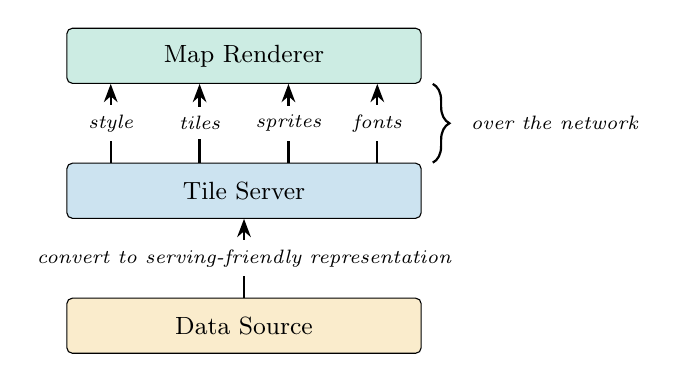
\begin{tikzpicture}[
		node distance=0.8cm and 1cm,
		box/.style={rectangle, draw, rounded corners=2pt, minimum height=0.7cm,
			minimum width=2.0cm, font=\small, align=center},
		renderer/.style={box, fill=roleGen!20, minimum width=4.5cm, minimum height=0.7cm},
		server/.style={box, fill=roleSrc!20, minimum width=4.5cm, minimum height=0.7cm},
		datasource/.style={box, fill=roleData!20, minimum width=4.5cm, minimum height=0.7cm},
		arrow/.style={-Stealth, thick},
		label/.style={font=\scriptsize\itshape, fill=white},
		]
		% Map Renderer (top)
		\node[renderer] (renderer) {Map Renderer};
		
		% Tile Server
		\node[server, below=1cm of renderer] (server) {Tile Server};
		
		% Arrows from server to renderer with resource labels
		\coordinate (s1) at ($(server.north)!0.25!(server.north east)$);
		\coordinate (s2) at ($(server.north)!0.75!(server.north east)$);
		\coordinate (s3) at ($(server.north)!0.25!(server.north west)$);
		\coordinate (s4) at ($(server.north)!0.75!(server.north west)$);
		
		\draw[arrow] (s4) -- node[label] {style}   (s4 |- renderer.south);
		\draw[arrow] (s3) -- node[label] {tiles}   (s3 |- renderer.south);
		\draw[arrow] (s1) -- node[label] {sprites} (s1 |- renderer.south);
		\draw[arrow] (s2) -- node[label] {fonts}   (s2 |- renderer.south);
		
		% "over the network" brace
		\draw[decorate, decoration={brace, amplitude=6pt}, thick]
		([xshift=4pt]renderer.south east) -- ([xshift=4pt]server.north east)
		node[midway, right=10pt, font=\scriptsize\itshape, align=left]
		{over the network};
		
		% Data Source (bottom)
		\node[datasource, below=1cm of server] (datasource) {Data Source};
		
		\draw[arrow] (datasource.north) -- node[label] {convert to serving-friendly representation} (server.south);
	\end{tikzpicture}
	\caption{
Basic building blocks of a map rendering stack.
Data is taken from a data source, converted into a simplified format (for example a spatial index), and served to a client.
The visual appearance is defined by a style and supported by fonts and sprites for text and icons.}
	\label{fig:basic-arch}
\end{figure}

As a lower-level representation layer for displaying map content, the following components are required, as shown in \cref{fig:basic-arch}.
\emph{Styles} define the visual appearance of the map and reference the other required resources.
\emph{Tiles} provide the geometry (points, lines, polygons) and associated attributes (for example, building heights) displayed on the map.
\emph{Sprites} supply the icons.
\emph{Fonts} provide the glyphs used to render text labels.
Occasionally, additional assets such as 3D geometry models or terrain are used as well.

There are several approaches to deliver client-side rendered vector maps.

Styles, sprites, and fonts are typically served from a file server or \ac{CDN} and require little processing.
In some cases, parts of these resources may be generated dynamically, for example to support complex text shaping for Arabic, Hebrew, Indic, or Japanese scripts as described by Wipfli~\cite{wipfliComplexTextPlugin2025} for MapLibre or Lengyel~\cite{lengelDecadeSlug} for SLUG.
This processing is currently usually handled ahead of time on the server-side.

Tiles, by contrast, can be stored and accessed using three major approaches:

\begin{description}
\item[\textbf{Dynamic}]
    Store geospatial data in a database (for example, PostGIS\footnote{\url{https://postgis.net/}, last accessed 2026-05-23}) and use a tile server to generate and serve tiles on demand.
\item[\textbf{Client-driven}]
    Store encoded tiles as a single file in a blob store using a format that includes an internal tile index (for example, PMTiles or VersaTiles).
    Clients retrieve tiles using multiple \ac{HTTP} requests with appropriate Range headers to locate the required data.
\item[\textbf{Semi-static}]
    Store encoded tiles in a database file on disk (for example, SQLite) and use a tile server to extract and serve tiles to clients.
\end{description}

Dynamic data sources can be updated frequently by applying incremental diffs, whereas the other approaches typically require a full rebuild when the underlying data changes.
At larger scales, in-memory caching of tiles via regional or \ac{CDN}-style infrastructure, combined with fallback to runtime-dynamic data, is essential for performance and cost.

Although all of these resources can be optimized, tiles are usualy the most critical due to their continuously streaming nature as a user moves the map.
They usualy have a cumulatively higher data volume due to this, even though their individual tiles may be much smaller.
All other resources may depend on locale slightly (for example loading different Unicode ranges or fonts), but are only handled one time.

Real-world observations support this:
the performance of highly optimized systems such as Microsoft Bing Maps differs significantly from less optimized deployments, such as basemap.de.

In the following sections we examine each resource in detail, focusing on the performance characteristics and optimization strategies relevant to our work:

\subsection{Fonts}

Fonts can be client rendered from a font file.
This requires shipping a text shaping engine to the client, as neither native nor web targets have for example Harfbuzz\footnote{\url{https://github.com/harfbuzz/harfbuzz}, last accessed 2026-05-26} exposed as a feature.
This also means that for some fonts up to \qty{131}{\mega\byte}\cite{FontThatIncludes} of font data needs to be transferred.

For interactive use cases, this is prohibitive as the time to download this would be longer than acceptable.
Some fonts need this shaping as they need to connect neigboring characters neatly, but Latin fonts do usually not.
For latin-like characters, there is usually a clear 1:1 relationship between the Unicode code point and a rendered character.

This is why a simpler way exists:
Cutting fonts up into Unicode slices (\texttt{start..end}) and serving only the ranges that are needed to the client.
This cutting of fonts has the implicit advantage of pruning the space of possible font data to just the data that is needed to render the map.

Common open-source renderers like MapLibre or source-available renderers like Mapbox do this by shipping pre-rasterised glyph ranges as \acp{PBF} encoded \acp{SDF}~\cite{greenImprovedAlphatestedMagnification2007}, indexed by Unicode range (e.g.\ \texttt{0-255.pbf}, \texttt{256-511.pbf}).

\subsection{Sprites}

Sprite rendering is a well-established technique in computer graphics.
To avoid having to request hundreds to thousands of small files or to have to render SVGs on a client, this work is shifted to the server and the server delivers sprite sheets.
This allows efficient \ac{GPU} Sprite instancing.

Common renderers like MapLibre or Mapbox do this by shipping plain \ac{PNG} or \acs{SDF}-\acs{PNG}~\cite{greenImprovedAlphatestedMagnification2007} sprite sheets together with a lookup table.
The lookup table records the location of each sprite, whether it is an SDF, and optional stretchable regions for symbols such as highway shields.

\subsection{Tiles}\label{sec:tiles}

Tiles are the primary data delivery mechanism for interactive web maps.
Rather than transferring the entire dataset to the client, the map is partitioned into a regular grid of square tiles at discrete zoom levels following the XYZ tiling scheme.

At zoom level~$z$, the world is subdivided into $2^z \times 2^z$ tiles, each identified by its column~$x$, row~$y$, and zoom level~$z$.
Lower zoom levels cover large geographic areas with simplified geometry with higher zoom levels cover smaller areas with greater detail.
The client requests only the tiles intersecting the current viewport, and as the user pans or zooms, new tiles are fetched while old ones are discarded or cached.
When a client requests a tile at a zoom level beyond the source's maximum, the renderer \emph{overzooms}: it upscales the nearest available tile from the source's highest available zoom to fill the viewport.

The \emph{layers} sourced from that tile remain rendered at the overzoomed level even though no new tile is fetched.
A layer's effective visibility at a given camera zoom is therefore a function of both the layer's filter and the source's \mlprop{maxzoom}, not the layer bounds alone.
This observation has direct consequences for any optimizer that rewrites zoom bounds.
Removing a layer at zoom~14, for example, will suppress its rendering at zoom~15 and beyond if the source's \mlprop{maxzoom} is~14, because the renderer continues to display overzoomed tiles from the highest available source zoom.
We turn this into the asymmetric \mlprop{minzoom}/ \mlprop{maxzoom} tightening rule in \cref{sub:structural_optimizations}.
\Cref{lst:overzoom} shows the two operations the slicer performs to synthezise a target tile from the source's \mlprop{maxzoom} tile.
\stepcirc{1}~Rescale each coordinate by $2^{\Delta z}$ relative to the target-tile offset ($offsetX \notin \{null,0\} \lor offsetY \notin \{null,0\} \Rightarrow x = x * scale - offsetX$). \stepcirc{2}~Clip to the target extent with a 128-unit overdraw buffer for continuous edge geometry.
Both operations consume the source's \mlprop{maxzoom} tile as input, which is what makes \mlprop{maxzoom} tightening risky in a way that \mlprop{minzoom} tightening is not.

\clearpage
\begin{lstlisting}[
  language=TypeScript,
  caption={Condensed MapLibre GL-JS overzoom implementation (\texttt{src/source/vector\_tile\_overzoomed.ts})},
  label=lst:overzoom,
  escapeinside={(*@}{@*)},
]
function sliceVectorTileLayer(sourceLayer, maxZoomTileID, targetTileID) {
    const {extent} = sourceLayer;
    const dz = targetTileID.z - maxZoomTileID.z;
    const scale = Math.pow(2, dz);

    // Target tile's offset within the source tile, in target coords
    const offsetX = (targetTileID.x - maxZoomTileID.x * scale) * extent;
    const offsetY = (targetTileID.y - maxZoomTileID.y * scale) * extent;

    for (const feature of sourceLayer) {
        let geometry = feature.loadGeometry();
        // (*@\stepcirc{1}@*) Rescale each coordinate into the target tile's space
        for (const ring of geometry) for (const p of ring) {
            p.x = p.x * scale - offsetX;
            p.y = p.y * scale - offsetY;
        }
        // (*@\stepcirc{2}@*) Clip to the target extent with a 128-unit overdraw buffer
        geometry = clipGeometry(geometry, feature.type,
                                -128, -128, extent + 128, extent + 128);
        // ...emit feature with rescaled+clipped geometry
    }
}
\end{lstlisting}

No symmetric \enquote{underzoom} behavior exists:
If a source has no tile at a zoom lower than \mlprop{minzoom}, the layer is  not rendered there.

A \emph{vector tile} encodes map data in a compact binary format rather than in a pre-rendered image.
Each tile is organized into \emph{source layers} (for example, roads, buildings, water), and each source layer contains a set of \emph{features}.
A feature consists of geometry (point, linestring, or polygon encoded as integer coordinates relative to the tile's extent), optionally a set of key-value \emph{properties} (for example, \texttt{class=motorway} or \texttt{name=Main~Street}), optionally a set of IDs, and metadata such as the tile extent.

The following formats are used for encoding and transferring data to the client:

\begin{description}
    \item[\textbf{Raster tiles}] deliver pre-rendered images (\ac{PNG}, JPEG, WebP, Avif, JPEGXL) rather than vector geometry.
    They require no client-side rendering logic but cannot be restyled, rotated at arbitrary angles (beyond the affine transform imposed by globe mode), or queried interactively, as the visual representation is fixed at generation time.

    \item[\textbf{Analysis-focused formats}] such as FlatGeobuf\footnote{\url{http://flatgeobuf.org/}, last accessed 2026-05-11}, GeoParquet\footnote{\url{https://geoparquet.org/}, last accessed 2026-05-11}, and GeoArrow are optimized for analytical queries (filtering, aggregation, joins) rather than tile-based rendering.
    GeoParquet's row-group predicate pushdown and column pruning are analogous to the tile shaving we apply to \ac{MLT}, but they operate at per-file granularity.
    Parquet's row-group and column-chunk metadata would dominate at typical tile sizes (\qtyrange{1}{10}{\kilo\byte}), so we do not consider these formats further.

    \item[\textbf{\ac{GeoJSON}}]~\cite{butlerGeoJSONFormat2016} is a \ac{JSON}-based geospatial interchange format.
    Its human-readable structure makes it useful for debugging and small overlays, but its verbosity (text-encoded coordinates and repeated property keys per feature) makes it impractical for the continuous tile streaming required by interactive map renderers.

    \item[\textbf{\acf{MVT}}]\footnote{\url{https://github.com/mapbox/vector-tile-spec/tree/master/2.1}, last accessed 2026-04-21} is the dominant vector tile format, adopted as a \emph{de~facto} standard across open-source map renderers including MapLibre.
    It uses the \ac{PBF}\footnote{\url{https://protobuf.dev/}, last accessed 2026-04-21} as its wire format and stores features in a \emph{row-oriented} layout:
\begin{itemize}
    \item Each \texttt{Feature} carries its own list of property tags encoded as alternating key and value indices into per-layer string and value tables.
    \item Geometry is encoded as a sequence of \texttt{MoveTo}, \texttt{LineTo}, and \texttt{ClosePath} commands with delta-encoded integer coordinates relative to the tile extent (typically \texttt{4096} units per tile edge).
    This is also known as "turtle style graphics"\footnote{\url{https://docs.python.org/3/library/turtle.html}, last accessed 2026-5-27} as an analogy to the \texttt{turtle} python module.
    \item The row-oriented layout means that accessing a single property column requires parsing past all other properties of the same \texttt{Feature}, and that compression operates on the interleaved byte stream rather than on homogeneous data columns.
\end{itemize}


    \item[\textbf{\acf{MLT}}] \begin{sloppypar} is a columnar vector tile format proposed by Tremmel et~al.~\cite{tremmelMapLibreTileNext2025b}.
    Instead of the row-major key-value-pair layout of \ac{MVT}, \ac{MLT} stores each property as an independent column with type-specific encoding.
    This columnar layout enables per-column compression strategies (for example, dictionary encoding for low-cardinality string columns, delta encoding for monotonically increasing integers, or run-length encoding for repeated values) and eliminates the per-feature tag overhead of the protobuf encoding.
    Tremmel et~al.\ report up to $3\times$ tile size reduction on encoded tilesets and up to $6\times$ on certain large tiles, with the realised ratio depending on data characteristics.\end{sloppypar}
\end{description}

Beyond the choice of tile format, a number of transfer-layer optimizations can improve delivery performance:
utilising the approximately \qty{14}{\kilo\byte} TCP slow-start window as discussed by Nathaniel~\cite{WhyYourWebsite}, edge caching\footnote{such as suggested by \url{https://docs.here.com/map-rendering/docs/cache-maps-raster-tile-api}, last accessed 2026-03-16}, HTTP/2 multiplexing~\cite{belsheHypertextTransferProtocol2015} (and its QUIC-based successor HTTP/3~\cite{bishopHTTP32022} for lossy mobile networks), and modern content-encoding algorithms such as Zstandard~\cite{colletZstandardCompressionApplication2021} and Brotli~\cite{alakuijalaBrotliCompressedData2016} that achieve higher compression ratios than gzip's LZ77 foundation~\cite{zivUniversalAlgorithmSequential1977}.
Tile archive formats such as PMTiles~\cite{PMTilesConceptsProtomaps} and COMTiles~\cite{tremmelCOMTILESCASESTUDY2023} address the container layer by enabling serverless, cloud-native tile delivery from a single file in blob storage.
Since \ac{MVT} is the established baseline and \ac{MLT} aims to improve upon it, we evaluate both formats and use the transition from \ac{MVT} to \ac{MLT} as one of our data-level optimization strategies.

\subsection{Styles}\label{sec:styles}

A map style defines the complete visual appearance of a map: which data is shown, how it is colored, sized, and labelled, and at which zoom levels each element appears.
Three architectural approaches to map styling have been established:

\begin{description}
    \item[\textbf{Server-side declarative}] styles, such as MapCSS, define rendering rules on the server.
    The server evaluates the style against the data and produces pre-rendered raster tiles that the client displays without further interpretation.
    This simplifies the clients rendering logic, but prevents client-side restyling and thus limits interactivity.

    \item[\textbf{Client-side declarative}] \begin{sloppypar} styles, as used by MapLibre\footnote{\url{https://maplibre.org/}, last accessed 2026-03-16} and Mapbox\footnote{\url{https://www.mapbox.com/}, last accessed 2026-03-16}, transmit a machine-readable style document to the client, which interprets the style at render time.
    This style can also be shipped with the code of the rendering engine to the client or partially constructed (e.g. road shields) there.
    This enables dynamic restyling, data-driven visualization, and interactive features such as hover effects and click queries without regenerating tiles.\end{sloppypar}

    \item[\textbf{Callback-based}] styling, as proposed by Gleo\footnote{\url{https://ivansanchez.gitlab.io/gleo/}, last accessed 2026-03-16} or Navara\footnote{\url{https://navara-docs.netlify.app/}, last accessed 2026-04-21}, replace declarative rules with imperative callbacks that the application registers with the renderer.
    This offers maximum flexibility but makes static analysis and automatic optimizations impossible, since the styling logic is opaque to the rendering engine.
\end{description}

We focus on client-side declarative styles, specifically the MapLibre style specification.
It is the most widely adopted approach in open-source map rendering, and its declarative nature makes it amenable to static analysis and automatic optimizations.

The MapLibre style specification\footnote{\url{https://www.maplibre.org/maplibre-style-spec/}, last accessed 2025-10-24} defines a map's appearance as a \ac{JSON} document with the following key components:

\begin{description}
    \item[\textbf{Sources}] declare where tile data comes from (tile server URL, or inline \ac{GeoJSON}) and at which zoom levels tiles are available (\mlprop{minzoom}, \mlprop{maxzoom}).

    \item[\textbf{Layers}] are the central rendering unit.
    Each layer references a source and a \emph{source-layer} within that source, specifies a \emph{type} (\texttt{\mlval{fill}}, \texttt{\mlval{line}}, \texttt{\mlval{circle}}, \texttt{\mlval{symbol}}, \texttt{\mlval{fill-extrusion}}, \texttt{\mlval{raster}}, \texttt{\mlval{background}} or \texttt{\mlval{hillshade}}) and carries a set of paint and layout properties that control its appearance.
    Layers are drawn in declaration order from bottom to top.
    \begin{description}

    \item[\textbf{Filters}] are boolean expressions attached to layers that select which features from the source-layer are rendered.
    A feature is drawn by a layer only if the layer's filter evaluates \mlval{true} for that feature's properties and geometry type.

    \item[\textbf{Paint and layout properties}] control the visual appearance and placement of rendered features.
    Paint properties (colors, opacities, widths) can be changed without triggering a re-layout.
    Layout properties (text anchoring, icon rotation, symbol spacing) affect feature placement and require re-evaluation when modified.

    \item[\textbf{Metadata bounds}] (\mlprop{minzoom}, \mlprop{maxzoom}) restrict the zoom range in which a layer is active.
    This allows the renderer to skip layers outside that range before filter evaluation or geometry decoding.
    \Cref{lst:ishidden} shows the corresponding \texttt{isHidden} guard.
    The worker invokes \texttt{layer.isHidden(this.zoom, true)} to skip bucket creation during tile parsing, while the renderer returns early from \texttt{renderLayer} on \texttt{layer.isHidden(this.transform.zoom)} before dispatching draw calls.
    
    \begin{minipage}{\dimexpr\linewidth\relax}
\begin{lstlisting}[language=TypeScript,caption={MapLibre GL-JS \texttt{isHidden} method from \texttt{src/style/style\_layer.ts}},label=lst:ishidden]
isHidden(zoom: number = this.minzoom, roundMinZoom: boolean = false) {
    if (this.minzoom && zoom < (roundMinZoom ? Math.floor(this.minzoom) : this.minzoom)) return true;
    if (this.maxzoom && zoom >= this.maxzoom) return true;
    return this._evaluatedVisibility === 'none';
}
\end{lstlisting}
\end{minipage}

\Cref{lst:ishidden_usage} reproduces the two call-sites that establish those two stages: the worker calls \texttt{layer.isHidden(this.zoom, true)} and \texttt{continue}s before bucket creation, and the painter's \texttt{renderLayer} returns immediately on \texttt{layer.isHidden(this.transform.zoom)} before dispatching any \texttt{draw.fill}/ \texttt{draw.line}/ \texttt{draw.symbol} call.
\end{description}
\end{description}

Filters and properties can be specified as literal constants, as \emph{zoom-dependent} expressions (varying with the camera zoom level via \mlop{interpolate} or \mlop{step} ramps), as \emph{data-driven} expressions (varying per feature based on property values via \mlop{match}, \mlop{case}, or \mlop{get} operators), or as a combination of both.
The resulting expression trees can be deeply nested and may contain redundant or unreachable branches.
These characteristics make them amenable to the same kinds of simplification and optimizations techniques used in compilers and database query planners.

\Cref{lst:worker_pipeline} shows the worker's tile-parse pipeline as five named steps, marked inline as \stepcirc{1} to \stepcirc{5}.

\noindent Every optimization we present in \cref{ch:methods} attaches to one of these steps.
Merging layers reduces work for \stepcirc{1}.
Pruning features server-side makes \stepcirc{2} not handle them.
Tightening \mlprop{minzoom}/ \mlprop{maxzoom} makes the \stepcirc{3} guard true earlier.
Pre-folding zoom-dependent constants reduces the work in \stepcirc{4}.
Filter-to-property propagation simplifies the per-feature work inside \stepcirc{5}.

\begin{lstlisting}[
    language=TypeScript,
    escapeinside={(*@}{@*)},
    caption={MapLibre GL-JS WorkerTile.parse processing pipeline (\texttt{src/source/worker\_tile.ts})},
    label=lst:worker_pipeline
]
// (*@\stepcirc{1}@*) Iterate source layers
const layerFamilies = layerIndex.familiesBySource[this.source];
for (const sourceLayerId in layerFamilies) {
    const sourceLayer = data.layers[sourceLayerId];
	if (!sourceLayer) continue;

    ...

    const sourceLayerIndex = sourceLayerCoder.encode(sourceLayerId);

    // (*@\stepcirc{2}@*) Collect raw features
    const features = [];
    for (let index = 0; index < sourceLayer.length; index++) {
        const feature = sourceLayer.feature(index);
        const id = featureIndex.getId(feature, sourceLayerId);
        features.push({feature, id, index, sourceLayerIndex});
    }

    for (const family of layerFamilies[sourceLayerId]) {
        const layer = family[0];

        ...
        // (*@\stepcirc{3}@*) Skip hidden layers
        if (layer.isHidden(this.zoom, true)) continue;

        // (*@\stepcirc{4}@*) Recalculate zoom-dependent expressions
        recalculateLayers(family, this.zoom, availableImages);

        const bucket = buckets[layer.id] = layer.createBucket({...});

        // (*@\stepcirc{5}@*) Filter features and build vertex data
        bucket.populate(features, options, this.tileID.canonical);
        featureIndex.bucketLayerIDs.push(family.map((l) => l.id));
    }
}
\end{lstlisting}

\subsection{Feature and Global State}\label{sub:feature_state}

A MapLibre map carries two runtime key-value stores that sit alongside the JSON style document and the encoded tile data, even though they live in neither.
\emph{Feature state} is a per-feature map keyed by the (source, source-layer, feature ID) triple, mutated from the host application via \texttt{setFeatureState} and \texttt{removeFeatureState}, and read from style expressions through the \texttt{[\mlop{"feature-state"},~key]} operator.
Its canonical use is interactive UI such as hover highlighting or click-driven selection.
\emph{Global state} is a map-wide key-value store mutated via \texttt{setGlobalStateProperty} and read through the \texttt{[\mlop{"global-state"},~key]} operator.
It typically backs up application-wide toggles such as a day/night switch or a per-mode road-class filter.

A state change re-evaluates the dependent paint expressions at render time, without re-parsing the tile or re-running bucket population.
This is what keeps feature state cheap enough to drive hover effects.
Both stores are mutated by the host application at runtime, after the style document and tile data have been loaded, so their values are not determined by either.
A reference whose key is missing from the store, or whose stored value has a type the consuming expression cannot handle, raises a runtime evaluation error that aborts rendering for the affected expression.
Feature-state addressing further requires stable feature IDs, since the keying triple includes the feature ID.

\section{Compiler Optimization Techniques}\label{sec:compiler_optimizations}

The style expressions used by map renderers such as MapLibre are small programs in a special purpose \ac{DSL}:
they contain conditionals (\mlop{case}, \mlop{match}), boolean operators (\mlop{all}, \mlop{any}), arithmetic, and data access (\mlop{get}, \mlop{has}), and variables (lexical bindings via \mlop{let}/ \mlop{var}, and the runtime stores of \cref{sub:feature_state}).
Optimising these expressions draws directly on techniques developed over decades in compiler construction~\cite{ahoCompilersPrinciplesTechniques2007}.
In this section we introduce the foundational concepts we apply in \cref{ch:methods}.

\subsection{Peephole Optimization}

\begin{sloppypar}
A \emph{peephole optimizer} examines a small, fixed-size window of code (the \enquote{peephole}) and applies local pattern-matching rewrites that replace instruction sequences with shorter or faster equivalents~\cite{davidsonCodeSelectionObject1984}.
Each rewrite rule is independent, matching a local pattern and emitting a replacement without requiring knowledge of the surrounding program.
Many small, local improvements compose into significant global optimizations under repeated application.
\end{sloppypar}

Peephole optimizers are classified by the level at which they operate.
\emph{Machine-level} peephole optimizers replace instruction sequences (e.g., replacing a multiply by a power of two with a shift).
\emph{\ac{IR}-level} peephole optimizers apply algebraic simplifications, identity eliminations, and strength reductions to expression trees.
In the context of style expressions, the peephole window corresponds to a single expression node and its immediate children.
A post-order visitor walks the expression tree and attempts to apply each rule at every node, producing a locally simplified tree.

\subsection{Constant Folding and Propagation}

\emph{Constant folding} evaluates expressions whose operands are all compile-time constants, replacing the expression with its result~\cite{ahoCompilersPrinciplesTechniques2007}.
For example, the expression $3 + 5$ is replaced by $8$.
In a style context, a comparison such as \texttt{[\mlop{"=="},~\mlval{2},~\mlval{3}]} can be evaluated at optimizations time and replaced by \mlval{false}.
\emph{Constant propagation} extends this idea by tracking the known values of variables through the program's control flow and substituting them at their use sites.
If a variable is assigned a constant, all subsequent references to that variable can be replaced by the constant, potentially enabling further constant folding at the use sites.

A more powerful variant, \acf{SCCP}, combines constant propagation with dead branch analysis in a single pass.
It simultaneously determines which values are constant \emph{and} which branches are reachable, enabling the discovery of constants that are only visible when unreachable code is ignored~\cite{wegmanConstantPropagationConditional1991}.

\subsection{Dead Code Elimination}

\acf{DCE} removes program statements whose results are never used or whose control-flow paths are unreachable~\cite{ahoCompilersPrinciplesTechniques2007}.
Two common forms are \emph{unreachable code elimination}, which removes code that can never be executed (e.g., code after a guaranteed return, or branches guarded by a statically false condition), and \emph{dead store elimination}, which removes assignments to variables that are never subsequently read.

In the map-style domain, dead code elimination corresponds to removing style layers that can never produce visible output, because their filter is unsatisfiable, their geometry type does not match the data, or their paint properties render them invisible (e.g., zero opacity at all zoom levels).

\subsection{Algebraic Simplification}

\emph{Algebraic simplification} applies mathematical identities to reduce expression complexity without changing semantics~\cite{ahoCompilersPrinciplesTechniques2007}.
Implemented algebraic rules include:

\begin{itemize}
	\item \emph{Identity elements}:
	\[
	\begin{alignedat}{4}
		x \land \mathit{true}   & = x \qquad &
		x \lor \mathit{false}   & = x \qquad &
		x + 0                   & = x \qquad &
		x \cdot 1               & = x
	\end{alignedat}
	\]

	\item \emph{Annihilation}:
	\[
	\begin{alignedat}{3}
		x \land \mathit{false}  & = \mathit{false} \qquad &
		x \lor \mathit{true}    & = \mathit{true} \qquad &
		\forall x \in \mathbb{N}: x \cdot 0               & = 0
	\end{alignedat}
	\]

	\item \emph{De~Morgan's laws}:
	\[
	\begin{alignedat}{2}
		\lnot (a \land b) & = \lnot a \lor \lnot b \qquad &
		\lnot (a \lor b)  & = \lnot a \land \lnot b
	\end{alignedat}
	\]

	\item \emph{Idempotence}:
	\[
	\begin{alignedat}{2}
		x \land x & = x \qquad &
		x \lor x  & = x
	\end{alignedat}
	\]

	\item \emph{Absorption}:
	\[
	\begin{alignedat}{2}
		x \land (x \lor y) & = x \qquad &
		x \lor (x \land y) & = x
	\end{alignedat}
	\]
\end{itemize}

\noindent For style expressions, these rules simplify boolean filter expressions.
A filter \texttt{[\mlop{"all"}, [\mlop{"all"}, a, b], c]} is flattened to \texttt{[\mlop{"all"}, a, b, c]} by associativity.
A filter \texttt{[\mlop{"all"}, \mlval{true}, x]} is simplified to~\texttt{x} by identity elimination.

\subsection{Fixpoint Iteration}\label{sub:fixpoint}

Individual peephole rules may expose further opportunities.
Constant folding a subexpression may create a new constant parent that enables dead branch elimination, so a single traversal is generally insufficient.

The remedy is to apply the entire rule set repeatedly until no rule fires.
A term to which no rule applies is a \emph{fixpoint} of the rewrite function, equivalently a \emph{normal form} of the underlying rewrite system.
We treat our expression-level optimizer formally as a \ac{TRS}~\cite{baaderTermRewritingAll1999}, which makes the relevant theoretical lens the pair of \emph{termination}\footnote{every reduction sequence reaches a normal point} and \emph{confluence}\footnote{all sequnences reach the same one} rather than the lattice-theoretic monotone-convergence framing of classical dataflow fixpoint iteration~\cite{ahoCompilersPrinciplesTechniques2007}.
\Cref{sub:expression_optimizations} gives a lexicographic measure on which most rules strictly decrease, together with the two rules (De~Morgan and distributive factoring) that can temporarily increase it, so a Knaster-Tarski-style convergence theorem~\cite{tarskiLatticetheoreticalFixpointTheorem1955} does not apply.

In practice the loop reaches a normal form within a handful of iterations and we cap it at eight as a safety bound.
Newcomb et~al.~\cite{newcombVerifyingImprovingHalides2020} reported similar confluence and termination concerns for Halide's hand-written rewrite optimizer and used synthezis-based techniques to verify correctness and discover missing rules.

\section{Query Optimization}\label{sec:query_optimizations}

Style filters in map rendering are structurally equivalent to database query predicates:
both select a subset of records (features) from a dataset (tile) based on attribute conditions.
Techniques from relational query optimizations therefore apply directly.

\subsection{Cost-Based Query Optimization}

A \emph{cost-based query optimizer} selects among semantically equivalent query execution plans by estimating the cost of each plan and choosing the cheapest~\cite{selingerAccessPathSelection1979}.

The key insight is that the \emph{order} in which predicates are evaluated affects performance even when the final result is identical.
Under short-circuit semantics, a conjunction $p_1 \land p_2 \land \cdots \land p_n$ is fastest when the most-likely-\mlval{false} predicate comes first, and a disjunction $p_1 \lor p_2 \lor \cdots \lor p_n$ places the most-likely-\mlval{true} predicate first.

\subsection{Selectivity Estimation}

Estimating the expected fraction of records satisfying a predicate is known as \emph{selectivity estimation}.
Selinger et~al.~\cite{selingerAccessPathSelection1979} introduced the foundational formulas for estimating selectivity under the \emph{independence assumption}, the assumption that attribute values in different columns are statistically independent.

For a single equality predicate $A = v$ on a column with $d$ distinct values, the estimated selectivity is $s = 1/d$ (uniform distribution assumption).
When value-frequency histograms are available, the estimate improves to $s = \mathit{freq}(v) / N$, where $N$ is the total number of records.
Compound predicates are estimated by combining individual selectivities:
\begin{align*}\label{eq:selectivity_theory}
    s(p_1 \land p_2) &= s(p_1) \cdot s(p_2)\\
    s(p_1 \lor p_2) &= 1 - (1 - s(p_1))(1 - s(p_2))
\end{align*}

The independence assumption is known to be inaccurate when columns are correlated, but it provides a computationally cheap approximation that is effective in practice~\cite{selingerAccessPathSelection1979}.
More sophisticated estimators (such as multi-dimensional histograms, sampling-based methods, or the lightweight graphical models proposed by Tzoumas et~al.~\cite{tzoumasLightweightGraphicalModels2011} that capture inter-attribute correlations without the full cost of joint-distribution estimation) improve accuracy at higher computational cost.

Map-style filters are in fact known to violate independence:
In OpenMapTiles, for example, \texttt{class} and \texttt{subclass} are strongly correlated by schema design (every value of \texttt{subclass} implies a constrained set of \texttt{class} values), as are \texttt{admin\_level} and \texttt{maritime}.
A joint-distribution estimator, such as the one we propose in \cref{sec:selectivity_reordering}, would therefore give tighter bounds, but our selectivity signal is consumed only by a \emph{reordering} heuristic (not by a cost-based plan chooser) and reordering is monotone in the ordering of the individual selectivities rather than in their absolute values.
The independence-estimator error therefore propagates into the quality of the short-circuit ordering but never into the correctness of the rewritten style, which makes the cheap estimator an acceptable engineering choice for our use case.

\subsection{Partial Evaluation}\label{sub:partial_eval}

\emph{Partial evaluation} (also called program specialization) transforms a program with respect to known static inputs, producing a residual program that depends only on the remaining dynamic inputs~\cite{jonesPartialEvaluationAutomatic1993}.
The style optimizer performs partial evaluation of the rendering function: the style (static input) is known at optimization time, while tile data (dynamic input) varies at runtime.
Filter-to-property constant propagation (\cref{sub:structural_optimizations}) is a textbook instance.
MapLibre paints only features that pass the filter (\cref{lst:bucket_populate}), so any equality constraint in the filter holds for every feature reaching the paint expression.
The optimizer substitutes that constraint into the paint expression and folds away the branches it rules out, while the filter itself stays unchanged and still runs at render time against dynamic feature data.
The same framing covers the stats-driven folding pass, where the tile's value distribution (cardinalities, per-property frequencies, geometry-type counts) is the additional static input that lets the optimizer collapse \mlop{match} arms over absent values, tighten zoom bounds, and convert high-selectivity predicates into constants.
This is distinct from profile-guided optimization, which would require measuring per-expression hotness at render time and specialising the hot paths.
The style optimizer never observes render-time execution and therefore does not perform that kind of specialisation.

The encoding strategy competition (\cref{sub:encoding_strategies}) is no partial evaluation but a single-output search.
It trials each candidate from a designer-specified set (sort orders $\times$ encoding schemes) on the actual data and emits the smallest, with a profiler pruning the search beforehand.
We characterise this as \emph{exhaustive strategy selection} over a bounded candidate space, optimal within that space but blind to strategies outside it.

\section{Data Encoding and Compression}\label{sec:data_encoding}

Efficient encoding of tile data is essential for interactive map performance, as tiles are fetched continuously during map interaction.
A column has to be both \emph{represented} as a value sequence and \emph{packed} into bytes, and some named schemes only address the first step while relying on the second to actually shrink the byte count.

Following the MLT specification, we call the first kind a \emph{logical-level technique} and the second a \emph{physical-level technique}.
A column applies zero or more logical techniques in chain and then exactly one physical technique, for example DeltaRLE~$\rightarrow$~FastPFOR.

\Cref{sub:logical_integer_encodings,sub:physical_integer_compressions} catalogue the techniques we use in our data-level optimizations of \cref{ch:methods}.

\subsection{Column-Oriented Storage}\label{sub:column_storage}

Traditional database systems store data in \emph{row-oriented} layouts, where all attributes of a single record are stored contiguously in memory.
This layout is efficient for transactional workloads that access entire records, but wasteful for analytical queries that access only a few columns, as the entire record must be read to access each single attribute.

\emph{Column-oriented} (columnar) storage transposes this layout, storing all values of a single attribute contiguously~\cite{abadiDesignImplementationModern2013}.
The foundational system in this space is by Dremel~\cite{melnikDremelInteractiveAnalysis}, who introducsed the record shredding and assembly algorithm for nested columnar data using definition and repetition levels, the representation pattern that directly inspired Apache Parquet and, by extension, the columnar layout that \ac{MLT} adapts for tile data.
This layout offers three advantages for read-heavy workloads. \emph{Reduced I/O} follows from reading or transferring only the referenced columns. \emph{Better compression} follows from the higher local homogeneity of values of the same type and semantic domain compared to interleaved multi-type records. \emph{Vectorised processing} follows from the layout's natural fit for \ac{SIMD}-style batch operations over arrays of the same type.

In the context of vector tiles, the row-oriented \ac{MVT} format stores all properties of a feature together, whereas the columnar \ac{MLT} format stores each property as an independent column.
The columnar layout allows per-column encoding strategies:
a column of \texttt{road} classes can use dictionary encoding, while a column of building heights can use a DeltaRLE logical chain handed to a physical technique such as FastPFOR, each chosen independently.

\subsection{Logical Integer Encodings}\label{sub:logical_integer_encodings}

Integer columns appear throughout tile data: geometry coordinates, feature IDs, property values, and dictionary indices.
Logical-level techniques rewrite the value sequence so that a downstream physical technique (\cref{sub:physical_integer_compressions}) sees a distribution that packs to fewer bytes.
Several such techniques exploit structural properties of integer sequences:

\begin{description}
    \item[\textbf{Zigzag encoding}] maps signed integers to unsigned ones ($n \mapsto 2n$ for $n \geq 0$, $n \mapsto -2n-1$ for $n < 0$) so that small-magnitude negative values also produce small unsigned codes.
    The byte count is unchanged on its own and the saving comes from the downstream physical technique.

    \item[\textbf{Delta encoding}] replaces each value with the difference from its predecessor: given a sequence $v_0, v_1, \ldots, v_n$, the encoded sequence is $v_0,\, v_1 - v_0,\, v_2 - v_1,\, \ldots,\, v_n - v_{n-1}$.
    Like zigzag, delta does not shrink the column by itself.
    It produces the same number of values at (often) smaller magnitude, which then pack well under VarInt or FastPFOR.

    \item[\textbf{\acf{RLE}}] replaces consecutive runs of identical values with (value, count) pairs.
    Unlike zigzag and delta, RLE reduces the symbol count on its own.
    MLT still classifies it as logical because it composes with other logical steps before a physical technique.
    It is most effective for low-cardinality, clustered columns, for example a road-class column sorted by class.
\end{description}

Logical techniques chain freely.
The canonical chain applies delta first and then \ac{RLE} (written DeltaRLE), effective for approximately sorted sequences where delta produces long runs of small (often zero) values that \ac{RLE} then collapses.

\subsection{Physical Integer Compressions}\label{sub:physical_integer_compressions}

A physical-level technique packs a value sequence (possibly the output of a logical chain) into bytes, and each integer column applies exactly one.
Our encoder uses two:

\begin{description}
    \item[\textbf{\acf{VarInt}}] represents each integer with a variable number of bytes, using 7~bits per byte for data and 1~bit as a continuation flag, so values in $[0, 127]$ take 1~byte, $[128, 16383]$ take 2~bytes, and so on\footnote{\url{https://protobuf.dev/}, last accessed 2026-04-21}.
    VarInt expects unsigned values, which is why a signed integer column is normally preceded by a zigzag remap.

    \item[\textbf{\acf{FastPFOR}}] partitions the input into fixed-size blocks (typically 128 or 256 values), computes the minimum bit width that fits most values in each block, and packs at that width, with outliers in a separate patch list~\cite{lemireDecodingBillionsIntegers2015}.
    This achieves near-optimal bit packing when most values share a similar magnitude.
\end{description}

Choosing the physical technique for a given logical chain has been studied systematically.
Abadi et~al.~\cite{abadiIntegratingCompressionExecution2006} proposed property-based selection rules, and Damme et~al.~\cite{dammeComprehensiveExperimentalSurvey2019} developed a cost-model-driven strategy that picks the lowest expected cost for a given data distribution.
A third school sidesteps both rule and model and decides empirically: BtrBlocks~\cite{kuschewskiBtrBlocksEfficientColumnar2023} trial-encodes candidate schemes on a sample of each column block and keeps the smallest result, arguing that lightweight on-sample trials are both more accurate than a cost model and cheap enough to run at encode time.
Our encoding competition in \cref{sub:encoding_strategies} sits in the same trial-based family.
It trials a pruned set of (logical chain, physical technique) pairs and retains the smallest output, but operates on each whole tile rather than on a sample, since per-tile data volumes are modest.

\subsection{String Compression}\label{sub:string_compression}

String data in vector tiles includes feature names, road classes, land-use categories, and administrative identifiers.
The same logical-then-physical split applies as for integer columns.

\textbf{Dictionary encoding} is the logical-level string technique.
It stores each unique string once and replaces occurrences with integer indices, which is effective when many features share the same value (e.g. thousands of features with \texttt{class = \texttt{residential}}).
The resulting index column is itself handed to the integer techniques of \cref{sub:logical_integer_encodings,sub:physical_integer_compressions}.

\textbf{\acf{FSST}}~\cite{bonczFSSTFastRandom2020} is the physical-level string technique.
It is a lightweight, block-oriented compressor that learns a \emph{symbol table} of up to 255 frequent byte sequences from the input corpus and replaces occurrences with single-byte codes.
Unlike general-purpose compressors such as LZ77~\cite{zivUniversalAlgorithmSequential1977a} or ~\cite{colletZstandardCompressionApplication2021}, \ac{FSST} preserves random access, so each compressed string can be decompressed independently.
The symbol table is stored once and amortised over all strings in the column.

The two compose in the same logical-then-physical pattern.
Applying \ac{FSST} to the deduplicated dictionary strings compresses both the unique values and the byte-level redundancy within them.

\subsection{Space-Filling Curves}\label{sub:space_filling_curves}

\emph{Space-filling curves} map multi-dimensional points to a one-dimensional ordering while preserving spatial locality.
Points that are close in two-dimensional space tend to receive nearby positions on the curve~\cite{moonAnalysisClusteringProperties2001}.
Such curves play two roles in tile encoding.
As a logical encoding they map a 2D coordinate to a single integer column (\cref{sub:logical_integer_encodings}).
As a \emph{feature ordering} they sort features before per-column encoding so that spatially adjacent features end up contiguous, improving the effectiveness of delta and \ac{RLE} on geometry and property columns.
This subsection treats the feature-ordering use.

Two space-filling curves are commonly used.

The \textbf{Z-order (Morton) curve}~\cite{morton1966computer} interleaves the binary representations of the $x$ and $y$ coordinates to form a single index.
For coordinates $(x, y)$ with $b$-bit components, the Morton code is
\begin{equation}\label{eq:morton}
    M(x, y) = \sum_{i=0}^{b-1} \bigl( x_i \cdot 2^{2i} + y_i \cdot 2^{2i+1} \bigr),
\end{equation}
where $x_i$ and $y_i$ are the $i$-th bits of $x$ and $y$, respectively.
Morton codes are fast to compute via bit-interleaving instructions, but the Z-order curve exhibits \enquote{jumps} between quadrants that break spatial continuity.

The \textbf{Hilbert curve} traces a continuous path through the grid without the inter-quadrant jumps of the Z-order curve, achieving better locality preservation at the cost of a more complex index computation~\cite{moonAnalysisClusteringProperties2001}.
The Hilbert curve has also been used as the basis for spatial index structures: the Hilbert R-tree~\cite{kamelHilbertRtreeImproved1994} orders rectangles along the Hilbert curve to achieve tighter node packing than conventional R-trees, and FlatGeobuf\footnote{\url{http://flatgeobuf.org/}, last accessed 2026-05-11} uses a packed Hilbert R-tree for spatial indexing of its features.
The Hilbert index is computed recursively.
The unit square is divided into four quadrants, each mapped to a sub-range of the curve.
The quadrant containing the point determines the high-order bits of the index, and the process recurses on the sub-quadrant.

For tile data, we assign each feature a curve index based on its first vertex coordinate, and our encoding competition described in \cref{ch:methods} selects the feature ordering that produces the smallest encoded output (across Morton, Hilbert, and non-spatial orderings).

\subsection{Locality-Sensitive Hashing}\label{sub:lsh}

When multiple string columns share overlapping vocabularies, storing a single shared dictionary can reduce overhead compared to per-column dictionaries.
Identifying which columns share sufficient overlap is a set similarity problem.

\emph{MinHash}~\cite{broderResemblanceContainmentDocuments1998} is a locality-sensitive hashing technique that estimates the \emph{Jaccard similarity} between two sets $A$ and $B$:
\begin{equation}\label{eq:jaccard}
    J(A, B) = \frac{|A \cap B|}{|A \cup B|}
\end{equation}
MinHash yields no asymptotic improvement over the exact computation.
Constructing a signature requires examining every element of $A$ and $B$, so the time complexity remains $\mathcal{O}(|A|+|B|)$, and the input sets must be retained throughout construction.
The reduction is a constant factor and applies to the persistent representation.
Whereas the exact computation stores all $\mathcal{O}(|A|+|B|)$ elements, MinHash stores only $k$ hash values per set.
For fixed $k$, the saving in persistent storage grows without bound as $|A|$ and $|B|$ increase.
For each of $k$ independent hash functions $h_1, \ldots, h_k$, the minimum hash value over all elements is recorded: $\mathit{sig}_i(A) = \min_{a \in A} h_i(a)$.
The Jaccard similarity is then estimated as:
\begin{equation}\label{eq:minhash}
    \hat{J}(A, B) = \frac{1}{k} \sum_{i=1}^{k} \mathbf{1}\bigl[\mathit{sig}_i(A) = \mathit{sig}_i(B)\bigr]
\end{equation}
where $\mathbf{1}[\cdot]$ is the indicator function.
The estimate is unbiased with variance $\mathcal{O}(1/k)$~\cite{broderResemblanceContainmentDocuments1998}, so the accuracy is fine-tunable.


\section{Benchmarking}\label{sec:benchmarking}

Benchmarking refers to the systematic measurement of system performance using controlled workloads and standardized metrics.
The purpose of benchmarking is to evaluate system behavior, compare alternative implementations, and quantify the effects of optimizations.

According to Jain~\cite{jainArtComputerSystems1991}, a good evaluation must start with selecting relevant metrics.
Georges et~al.~\cite{georgesStatisticallyRigorousJava2007} later demonstrated that naive averaging of execution times on managed runtimes (such as JavaScript engines) leads to unreliable conclusions, advocating instead for confidence intervals computed over multiple independent \ac{JVM}/engine invocations.
That principle informs the bootstrap CI methodology we use.
The bootstrap itself, a resampling method for constructing confidence intervals without distributional assumptions, was formalised by Efron and Tibshirani~\cite{efronIntroductionBootstrap1998} and is the specific statistical technique we apply throughout our evaluation (\cref{ch:experiments}).
Hoefler and Belli~\cite{hoeflerScientificBenchmarkingParallel2015} codified twelve common pitfalls in reporting performance results.
Our evaluation in \cref{ch:experiments} follows their guidelines by reporting per-metric confidence intervals and separating throughput from latency measurements.
In the context of web maps, the candidate metrics span a range from deployment-critical on battery-constrained targets to directly user-visible ones on the desktop:

\begin{description}
    \item[\textbf{Resource utilisation,}] such as \ac{CPU} load, \ac{GPU} utilisation, and memory consumption to have pointers where further optimizations is possible.
    \item[\textbf{Latency and responsiveness,}] measuring the time between initiating an operation (for example zooming) and the first visible result.
    \item[\textbf{Throughput,}] typically measured in \acp{FPS} or frame time, describing how many frames can be rendered per second.
    \item[\textbf{Frame stability,}] which captures variations in frame time and identifies dropped frames or rendering stutters.
    \item[\textbf{Network utilisation,}] including transferred bytes, tile request rates, and bandwidth consumption.
    \item[\textbf{Power consumption}] in Watts, which is relevant for mobile devices and battery-powered systems.  We do not measure power consumption.
We use no \ac{RAPL} counters, battery deltas, or external power meters, as our benchmark host is a desktop workstation rather than a battery-constrained mobile device.  We list power here as a candidate metric because transfer-size reductions and reduced draw-call counts are established proxies for energy savings on mobile targets.
Cellular radio energy is proportional to data volume, and \ac{GPU} active time scales with draw-call count.
\end{description}

These can be benchmarked at different workload levels~\cite{jainArtComputerSystems1991}:

\begin{description}
    \item[\textbf{Micro-benchmarks}] isolate a single operation (e.g.\ decoding a single tile, evaluating a single filter expression) and measure its cost in isolation.
They are useful for identifying bottlenecks but may not reflect real-world performance due to caching and concurrency effects.
    \item[\textbf{Macro-benchmarks}] measure the performance of a complete subsystem (e.g.\ loading a full style and rendering a fixed camera path) under controlled conditions.
They capture interactions between components but require careful setup to ensure reproducibility.
    \item[\textbf{Application-level benchmarks}] measure end-to-end user-perceived performance (e.g.\ time from page load to interactive map) in a realistic deployment.
They are the most representative but also the noisiest due to network variability, browser behavior, and hardware differences.
\end{description}

\noindent We primarily use macro-benchmarks: we load a full style, fetch and decode tiles, and exercise the renderer with a scripted camera animation.
Our benchmark harness controls for network variability (via a caching proxy) and \ac{GPU} variability (via hardware-accelerated rendering with ANGLE/Vulkan) to achieve reproducible results at the macro level.

\begin{chaptersummary}
Three theoretical traditions map onto the three levels of the pipeline.
\textbf{Compiler optimization} (peephole rewriting, constant folding, fixpoint iteration) drives the expression-level passes that simplify each style's \ac{JSON} expressions without schema knowledge.
\textbf{Query optimization} (projection pushdown, selectivity estimation) shapes the structural passes and the pruning advisory that bridges style and data.
The \textbf{encoding techniques} surveyed last feed the data-level passes that re-encode shaved tiles with automatic strategy selection.
These cover columnar storage, the logical encodings (zigzag, delta, \ac{RLE}, dictionary) and physical techniques (VarInt, FastPFOR, \ac{FSST}) they hand off to, and space-filling curves.
We adopt the benchmarking literature's statistical methodology (bootstrap confidence intervals, warm-up handling, metric separation) rather than extending it.

The following chapter formalises the joint optimization problem (\cref{sec:problem_statement,sec:scope}) and turns these foundations into concrete passes (\cref{sec:approach,sec:building_optimizations}) and an evaluation methodology (\cref{sec:gathering_sample,sec:evaluation}).
\end{chaptersummary}

\chapter{Methods}\label{ch:methods}

The preceding chapters established that no existing tool jointly optimizes map styles and tile data, and introduced the compiler, database, and encoding techniques whose analogues make such joint optimization possible.
This chapter applies those foundations in a concrete Rust optimizer that consumes a MapLibre style~\ac{JSON} document with optional tile statistics and emits a visually equivalent style with optimized tile data.
We formalise the problem and its visual-equivalence constraint (\cref{sec:problem_statement}), scope the work to MapLibre GL~JS (\cref{sec:scope}), and then walk level by level through the three-level pipeline (\cref{sec:approach}) and the passes that implement it.

\section{Formalised Problem Statement}\label{sec:problem_statement}

With the foundations of \cref{ch:theoretical_background} in place, we state the optimization problem formally.

Let $\mathcal{S}$ be the set of syntactically valid MapLibre style~\ac{JSON} documents.\newline
Let $\mathcal{T}$ be the set of tile sets, each a finite family of tiles indexed by source and $(x, y, z)$.\newline
Let $\mathcal{V}$ be the set of \emph{viewing states}: tuples $(\text{lat}_\text{center}, \text{lat}_\text{center}, z, \text{roll}, \text{pitch}, \text{bearing}, \text{viewport size})$, the six degrees of freedom plus the viewport.\newline
Let $\mathcal{I}$ be the set of rasterised images and let $\bot \notin \mathcal{I}$ denote a runtime evaluation error that aborts rendering, as introduced for ill-formed feature-state and global-state references in \cref{sub:feature_state}.
Let MapLibre's deterministic rendering function be
\begin{equation}\label{eq:render_function}
    R : \mathcal{S} \times \mathcal{T} \times \mathcal{V} \to \mathcal{I} \cup \{\bot\}
\end{equation}

The optimizer is a function $\mathcal{O}: \mathcal{S} \times \mathcal{T} \to \mathcal{S} \times \mathcal{T}$ with $(S', T') = \mathcal{O}(S, T)$.
$\mathcal{O}$ pays a one-off preprocessing cost $C_\text{total}(S, T)$, analytically decomposed and bounded in \cref{sub:preprocessing_cost_model}, in order to improve the deployment metrics of \cref{sub:metrics} (load time, heap memory, FPS, with finer-grained diagnostics) for every subsequent rendering session served from $(S', T')$.
The deployment cost is intentionally not formalised as a single closed-form function: it depends on hardware, camera scenario, and tile cache state, and is therefore measured empirically rather than declared analytically.
$\mathcal{O}$ is correspondingly not posed as a single-objective minimisation.
Several passes (e.g.\ selectivity reordering, \cref{sub:expression_optimizations}) deliberately trade a small regression in load time for a larger improvement in FPS, and the encoder competition (\cref{sub:encoding_strategies}) locally minimises encoded byte size as a contributing quantity to load time without committing to any weighting between the deployment axes.
We characterise each pass empirically against the metric battery of \cref{sub:metrics} in the ablation of \cref{ch:experiments}, and the resulting per-axis breakdown is what lets an operator compose the pass set that suits the deployment priorities.

$\mathcal{O}$ must satisfy two formal constraints.
The first constraint is \emph{visual equivalence}.
Writing $\equiv$ for pixel-identity on $\mathcal{I}$,
\begin{equation}\label{eq:visual_equivalence}
    \forall v \in \mathcal{V}:\; R(S, T, v) \neq \bot \;\Rightarrow\; R(S', T', v) \equiv R(S, T, v).
\end{equation}
The constraint is asymmetric in $\bot$.
An optimisation pass may suppress a runtime evaluation error that the original style would have raised, but it must never introduce one that the original would not have raised.
In practice we sample $v$ on a discrete grid of zooms and viewports, and check $\equiv$ by direct image comparison rather than by formal proof.
\Cref{eq:visual_equivalence} doubles as the \emph{soundness criterion} for every pass in this chapter.
Any rewrite whose correctness depends on a MapLibre runtime invariant must either preserve the invariant or reject the rewrite when the invariant cannot be established.

For example, the stats-driven folding pass cannot soundly remove a \mlop{match} arm without a full census of the tile data, because the arm may be reached by features the statistics have not observed.
The pass is consequently gated on a sample rate of~1.0.
Similarly, the metadata-refinement pass must reason about overzoom (\cref{sec:tiles}) when tightening \mlprop{maxzoom}, because an overzoomed tile counts as a viewing state in \cref{eq:visual_equivalence}.

The second constraint is \emph{strict idempotency}:
\begin{equation}\label{eq:idempotency}
    \quad \forall (s, t) \in \mathcal{S} \times \mathcal{T}: \mathcal{O}(\mathcal{O}(s, t)) = \mathcal{O}(s, t)
\end{equation}
Feeding $\mathcal{O}$'s output back as input yields the same pair, ruling out unbounded chained improvement by construction.
The expression-pass fixpoint of \cref{sub:fixpoint} enforces idempotency on the style half.
The deterministic, statistics-driven encoding choices of \cref{sub:data_optimizations} enforce it on the tile half.
Both halves are exercised on the style level by the round-trip proptest and on the tile level by the proptest+libFuzzer harness of \cref{par:encoder_validation}.

\section{Scope}\label{sec:scope}

We target MapLibre GL~JS as the system under test.
As discussed in \cref{sec:styles}, performance research on interactive vector maps is concentrated on Mapbox and MapLibre styles.
The Mapbox codebase is proprietary and may not be evaluated without explicit consent, leaving MapLibre as the only viable open research target.
Within MapLibre, the web renderer \texttt{maplibre-gl-js} is the reference implementation that first tracks new specification features and exposes the richest instrumentation hooks for Puppeteer-driven benchmarking, which is what makes it our benchmark target rather than the Native or mobile renderers that share the same styling engine.

In scope are the three pass families that make up the optimizer pipeline (\cref{sub:pipeline}): expression-level rewrites on style~\ac{JSON} (constant folding, algebraic simplification, statistics-driven folding, selectivity reordering), structural rewrites over a typed style model (dead-layer elimination, metadata refinement, layer merging), and data-level rewrites on the served tile payload (style-driven tile shaving and \ac{MLT} encoding-strategy selection).
Style and data passes are co-designed so that data rewrites are advised by the optimized style, and every pass is bound by the visual-equivalence constraint of \cref{eq:visual_equivalence} as its soundness criterion.

The following concerns are deliberately out of scope:

\begin{description}
    \item[\emph{Energy measurement}] Energy effects are discussed only qualitatively.
We report no \ac{RAPL} or battery deltas because the benchmark host is a desktop workstation rather than a mobile device (\cref{sub:metrics}).
    \item[\emph{Lossy geometry transformations}] Coordinate-precision reduction, Visvalingam-Whyatt, Douglas-Peucker, and polygon coalescing would violate the pixel-identity contract of \cref{eq:visual_equivalence}.
    Writing a visually non-lossy gepgraphic simplification is deferred to future work.
    We therefore quantify the size reductions achievable \emph{without} touching geometry, understating that there is headroom that composition with an geographic simplifier could reach at the cost of changing the style output.
    \item[\emph{Symbol-layer merging}] MapLibre evaluates symbol placement per layer through a tile-wide\newline
    \noindent\texttt{CollisionIndex}, so merging symbol layers would alter label suppression order.
The detailed argument is given along the structural passes (\cref{sub:structural_optimizations}).
    \item[\emph{Proprietary style corpora}] Mapbox Streets, Esri vector basemaps, and similar commercial styles are excluded by their terms of service.
    \item[\emph{Tile schemas other than \ac{OMT}}] Non-\ac{OMT} vector tile sources are excluded from the deep-corpus evaluation, and the stats-driven thresholds used by the pipeline are tuned on Germany~\ac{OMT} only (\cref{sec:gathering_sample}).
    \item[\emph{Online and incremental serving}] The optimizer is an offline, one-shot rebuild over a (style, tile~set) pair.
No integration with a live tile server is assumed, and the optimized artefacts can be served by any standards-compliant tile infrastructure.
    \item[\emph{The reference \ac{MLT} encoder}] The legacy self-contained \ac{MLT} encoder of Tremmel~\&~Zink~\cite{tremmelMapLibreTileNext2025b} is retained as a baseline for the encoding experiments of \cref{ch:experiments}.
It is not a target of optimization in this thesis.
\end{description}

\section{Approach and Basic Building Blocks}\label{sec:approach}

To evaluate the effectiveness of the optimizations strategies developed in this work, we adopted a benchmarking-driven approach.
We first established a reliable performance baseline and then ran cumulative ablation experiments that isolate the contribution of each optimizations pass.
Under the soundness contract of \cref{sec:scope}, the passes from~\cref{sub:pipeline} aim to improve the deployment metrics of \cref{sub:metrics} in exchange for the preprocessing cost $C_\text{total}$ of \cref{sub:preprocessing_cost_model}.
The load-time / FPS trade-off underlying these metrics is discussed in \cref{sec:problem_statement}.

\subsection{Three-Level Optimization Pipeline}\label{sub:pipeline}

\Cref{fig:system_architecture} sketches the optimizer system as a whole.
At the centre sits the \emph{optimiser}, a pipeline of passes at three levels of abstraction.
Around the optimiser are three supporting components, each detailed in its own section.
A code-generation front end (\cref{sub:codegen}) produces Rust types from the upstream MapLibre style specification.
A tile-statistics scanner (\cref{sub:tile_statistics}) profiles \ac{MVT} tiles for the stats-driven and data-level passes.
A validation harness (pixel-exact render tests plus a curated style corpus) exercises both pipelines against the visual-equivalence guarantee of \cref{eq:visual_equivalence}.
The three pass levels at the centre are:

\begin{enumerate}
    \item \textbf{Expression passes} (\cref{sub:expression_optimizations}) operate directly on the \ac{JSON} representation of style expressions, applying peephole rewrites, constant folding, and algebraic simplifications (\cref{sec:compiler_optimizations}) without deserializing the style into typed structures.
    They run to a fixpoint with a hard cap of eight iterations.
    In practice every style in the benchmarking and Maputnik\footnote{\url{https://maputnik.github.io/}, last accessed 2026-05-23} corpora converges within two to three iterations, well below the cap, because human-authored styles tend to reuse a small repertoire of patterns.
    The formal termination measure and confluence (\cref{sub:fixpoint}) discussion are given alongside the pass descriptions.
    \item \textbf{Structural passes} (\cref{sub:structural_optimizations}) deserialize the style into the typed Rust spec produced by the codegen front end and apply transformations that require cross-layer or cross-source reasoning, namely dead layer elimination, metadata refinement, layer merging, and cleanup.
    A cross-phase \emph{filter-to-property constant propagation}, which substitutes equality constraints extracted from a layer's filter into that layer's paint and layout expressions, bridges the expression and structural phases and is detailed in \cref{sub:structural_optimizations}.
    \item \textbf{Data passes} (\cref{sub:data_optimizations}) transform the served tile data via a style-driven pruning advisory and the conversion from \ac{MVT} to \ac{MLT}.
\end{enumerate}

\noindent We chose this ordering to address the \emph{phase ordering problem}~\cite{clickCombiningAnalysesCombining1995}.
Expression passes run first, allowing subsequent structural passes to operate on simplified expressions.
Dead elimination then removes unused layers before layer merging, creating additional merging opportunities.
Finally, the data phase processes the fully optimized style so that pruning recommendations are based on the final set of live layers and properties.

\begin{figure}[htbp]
    \centering
    \begin{tikzpicture}[
        node distance=0.8cm and 1.4cm,
        box/.style={rectangle, draw, rounded corners=2pt, minimum height=0.7cm,
                    minimum width=2.0cm, font=\small, align=center},
        src/.style={box, fill=roleSrc!20},
        mir/.style={box, fill=roleMir!30},
        gen/.style={box, fill=roleGen!20},
        data/.style={box, fill=roleData!25},
        opt/.style={box, fill=roleOpt!35, minimum width=2.4cm},
        test/.style={box, fill=roleTest!25},
        arrow/.style={-Stealth, thick},
        query/.style={-Stealth, thick, densely dashed},
        label/.style={font=\scriptsize\itshape, text=darkgray},
        validationlabel/.style={font=\scriptsize\itshape, text=cvdvermillion},
        validation/.style={
            dashed,
            cvdvermillion,
            ->,
            every edge node/.append style={text=cvdvermillion}
        },
    ]
        % Codegen pipeline (top row)
        \node[src]  (v8)     {\texttt{v8.json}};
        \node[mir,  right=of v8]   (parsed) {ParsedSpec};
        \node[mir,  right=of parsed] (mir)    {MIR};
        \node[gen,  right=of mir]  (serial) {SerialSpec\\{\scriptsize (generated Code)}};

        \draw[arrow] (v8)     -- node[above, label] {decode} (parsed);
        \draw[arrow] (parsed) -- node[above, label] {normalize} (mir);
        \draw[arrow] (mir)    -- node[above, label] {generate} (serial);

        % Data pipeline (bottom row)
        \node[src, below=2.5cm of v8] (proto) {Protobuf\\{\scriptsize (\acs{MVT})}};
        \node[data, right=of proto] (mvt) {MVTLayer};
        \node[data, right=of mvt]   (scan) {DataScanner};

        \draw[query] (proto) -- node[above, label] {decode} (mvt);
        \draw[query] (mvt)   -- node[above, label] {scan tiles} (scan);

        % tangled nodes
        \node[opt, below=2.5cm of serial] (opt) {Optimiser};
        \node[test] (test)  at ($(serial)!0.5!(opt) + (3cm,0)$)  {Render tests};
        \node[test, below=1cm of mir] (corpus) {Style Corpus};

        % tanlged arrows
        \draw[<->,double,thick,densely dashed] (opt) -- node[left,black] {\scriptsize\itshape optimize} (serial);
        \draw[query] (scan) -- node[above, label] {statistics} (opt);
        \draw[validation] (corpus) -- node[left, validationlabel] {validate} (serial);
        \draw[validation] (corpus) -- node[left, validationlabel] {eval} (opt);
        \draw[validation] (test) -- node[right, validationlabel] {validate} (serial);
        \draw[validation] (test) -- node[right, validationlabel] {validate} (opt);
    \end{tikzpicture}
    \caption{
System architecture.
    The \emph{codegen pipeline} (top) transforms the upstream \texttt{v8.json} style specification through three stages into generated Rust types (\texttt{SerialSpec}) used for typed style manipulation, with the MIR providing spec metadata to the optimizer.
    The \emph{data pipeline} (bottom) decodes \acs{MVT} tiles and scans them to produce tile statistics that feed into data-driven optimizations passes.
Render tests validate round-trip correctness and the style corpus is used to both validate the codegen and evaluate the optimizer.}
    \label{fig:system_architecture}
\end{figure}

\subsection{Code Generation from v8.json}\label{sub:codegen}

We design structural passes to operate on Rust types \emph{generated} from the upstream MapLibre GL~JS style specification rather than raw \ac{JSON}.
This shifts spec drift from a manual synchronisation burden to a regenerator invocation, and gives every pass typed access to defaults, value types, and expression capabilities.
Hand-written Rust types are not a viable alternative: MapLibre publishes the specification in its own \ac{JSON}-based \ac{DSL}, and a hand-maintained shadow would require manual synchronisation with every specification change and risk silent divergence.

The generation pipeline (top row of \cref{fig:system_architecture}) proceeds in three stages.
First, it \emph{decodes} the published \texttt{v8.json} into an internal representation.
Second, it \emph{normalizes} the result into a stable intermediate representation (the \texttt{MIR}\footnote{The \texttt{MIR} draws on the normalized-IR design of MLIR~\cite{lattnerMLIRScalingCompiler2021}, providing a stable form between upstream sources and downstream consumers (the codegen emitter and the structural passes).
The dialect, lowering, and pass-manager machinery of the full MLIR framework is not carried over.
The optimizer operates at a single abstraction level with no code-generation target, and round-trips its output to JSON for unmodified MapLibre renderers.}) that resolves cross-cutting concerns.
In particular, it collapses paint and layout properties that the spec defines across multiple sections into per-layer field definitions carrying type, default, and expression-capability metadata.
Third, a code emitter \emph{generates} Rust sources with round-trip serialization support.

This metadata is the substrate for two structural passes.
Layer merging queries the MIR to decide whether a differing paint property supports feature-driven expressions (and can therefore be wrapped in a \mlop{case}/ \mlop{match} over the filter discriminator) or is camera-only and must remain uniform across merged layers.
Default stripping compares property values against the specification defaults encoded in the generated types.

\subsection{Implementation}\label{sub:implementation}

The style optimizer is a standalone Rust binary.
The tile re-encoder described in \cref{sub:data_optimizations} shares the same Cargo workspace and is split into a core encoder/decoder crate and a Java wrapper crate so that a \ac{JVM}-based tile-generation pipeline can consume the encoder without re-implementing it.
The cross-language surface is generated by \emph{Diplomat}\footnote{\url{https://github.com/rust-diplomat/diplomat}, last accessed 2026-05-11}, which produces idiomatic, language-specific bindings directly from annotated Rust types, replacing the earlier \texttt{cbindgen}\footnote{\url{https://github.com/mozilla/cbindgen}, last accessed 2026-05-23}/\texttt{jextract}\footnote{\url{https://github.com/openjdk/jextract}, last accessed 2026-05-23} approach.
The Java wrapper exposes the generated bindings through the Panama \ac{FFM} \ac{API} (JEP~454)\footnote{\url{https://openjdk.org/jeps/454}, last accessed 2026-05-23} rather than conventional \ac{JNI} glue, eliminating hand-written C stubs and giving the \ac{JVM} direct, zero-copy access to off-heap buffers.
This is the boundary shape a columnar encoder requires: each tile is handed over as a batch of parallel \texttt{MemorySegment}s rather than one call per feature, amortising the per-boundary cost over thousands of features in one encoder invocation.

\section{Building Optimizations}\label{sec:building_optimizations}

The implemented passes target three areas of the rendering pipeline: style expressions, structural properties, and tile data.
We classify each pass by \emph{where} it operates and its \emph{data requirements} (none, sampling, or full scan).
Many are analogues of well-known compiler and query-processing techniques.

Each level discharges the visual-equivalence contract of \cref{sec:scope} in a different way.
For expression-level passes, the termination measure $\mu(S)$ (\cref{eq:termination_measure}) witnesses this.
Each rewrite strictly reduces $\mu$ while preserving expression semantics.
For structural passes, we argue soundness per-pass in the paragraphs below.
Dead elimination preserves equivalence because it only removes layers that produce no visible output.
Metadata refinement preserves equivalence because it only tightens bounds that the renderer would enforce anyway (with the overzoom asymmetry detailed below).
Layer merging preserves equivalence via the three invariants of \cref{sub:structural_optimizations}.
For data-level passes, the pruning advisory removes only data that no live style layer references, so the rendering function $R$ receives the same effective input.

\subsection{Expression-Level Optimizations}\label{sub:expression_optimizations}

Expression passes operate directly on the \ac{JSON} representation, applying rewrites that reduce expression complexity and eliminate redundant computation.
\cref{tab:expression_passes} summarizes the implemented passes.

\begin{table}[htbp]
\centering
\begin{tblr}{
  colspec = {p{3.8cm} p{1.8cm} p{9.5cm}},
  rows = {font=\small},
  row{1} = {font=\small\bfseries},
}
\toprule
Pass & Data & Description [compiler analogy] \\
\midrule
Unary simplification         & none     & Unwrap single-argument \mlop{any}/ \mlop{all} wrappers [identity elimination] \\
Expression kind normalization & none     & Rewrite negated comparisons to their direct form, e.g.\ \texttt{[\mlop{"!"}, [\mlop{"=="},a,b]]} $\to$ \texttt{[\mlop{"!="},a,b]} [operator strength reduction] \\
Constant folding              & none     & Evaluate statically determinable expressions: boolean algebra, dead branch elimination, redundant coercion removal [constant folding, \acs{SCCP}] \\
Stats-driven constant folding & sampling & Fold \mlop{has}/ \mlop{get}/ \mlop{geometry-type} expressions using tile statistics; prune unreachable \mlop{match}/ \mlop{in} arms; fold comparisons against known value ranges [sparse conditional constant propagation] \\
Expression simplification     & none     & De~Morgan's laws, boolean flattening, coalesce flattening, \mlop{case}$\to$\mlop{match} rewriting, \mlop{let}/ \mlop{var} inlining, \mlop{any}$\to$\mlop{in} merging, interpolate/step collapsing [algebraic simplification] \\
Default stripping             & none     & Remove paint/layout properties whose value equals the specification default [dead store elimination] \\
Colour minification           & none     & Compress color literals to their shortest representation [literal compression] \\
Selectivity reordering        & sampling & Reorder filter predicates by selectivity so the most discriminating condition is evaluated first [predicate reordering] \\
\bottomrule
\end{tblr}
\caption{
Expression-level optimization passes, each annotated with its data dependency (\emph{none} = static only; \emph{sampling} = requires a tile-statistics scan) and its compiler-optimization analogue.  Passes requiring no statistics run unconditionally.
Sampling passes additionally fold expressions using observed value distributions.}
\label{tab:expression_passes}
\end{table}

Among these passes, we expect constant folding to dominate because reducing an expression to a literal eliminates all per-feature evaluation cost.
The other passes primarily shorten the evaluation path rather than eliminating it.

We organize the expression pass engine as a table of rewrite rules (\cref{tab:all_rewrite_rules}), each gated by a \emph{pass flag} (which pass must be enabled) and scoped to a \emph{rule scope} (whether the rule applies to filters only, to paint/layout properties, or to both).
Selectivity reordering runs as a separate pass after the rewrite table has stabilised.
We further classify rules by their \emph{type}:
	\emph{pure} rules operate on the expression array alone,
	\emph{MIR-aware} rules additionally consult the specification's type metadata (e.g.\ to determine whether an operator is pure or to look up default values), and
	\emph{stats-driven} rules are recursive tree folds that receive tile statistics and layer-level context.
A post-order visitor walks every expression node in the style.
At each node, it tests all applicable peephole rules and the first matching rule fires.
Stats-driven rules run as separate tree folds after the peephole pass, because they require recursive context threading that the node-local peephole architecture does not provide.
We modeled this architecture on peephole optimizers in production compilers.
Individual rules are simple and local, but their composition through fixpoint iteration (\cref{sub:fixpoint}) achieves global simplifications.

\paragraph{Constant Folding}
The constant folding pass implements 17~rewrite rules that collectively perform the role of constant propagation and dead code elimination in a compiler (\cref{sec:compiler_optimizations}).
Boolean algebra rules evaluate \mlop{all}/ \mlop{any} nodes with known operands: a vacuous \texttt{[\mlop{"all"}]} rewrites to \mlval{true} (vacuous truth), a vacuous \texttt{[\mlop{"any"}]} to \mlval{false} (vacuous disjunction), and boolean absorption removes known-true operands from \mlop{all} and known-false operands from \mlop{any}.
Absorption is sound because MapLibre filter operators are pure (the filter language exposes no feature-state mutation, see \cref{sub:feature_state}), so dropping an operand cannot discard an observable side effect, and the asymmetric form of \cref{eq:visual_equivalence} permits dropping an operand whose evaluation would have raised $\bot$.
Comparison rules evaluate binary comparisons with two literal operands.
Dead-branch elimination removes arms from \mlop{case} and \mlop{match} expressions whose guard is statically false.

Contradiction detection identifies filters that are logically unsatisfiable by inspecting siblings within an \mlop{all} node.
When two predicates constrain the same property to disjoint values, e.g.

\begin{lstlisting}[
	style=maplibrestyle,
	basicstyle=\ttfamily\scriptsize,
	frame=single,
	aboveskip=5pt,
	belowskip=5pt
	]
["all",
	["==", ["get", "class"], "a"],
	["==", ["get", "class"], "b"]
]
\end{lstlisting}

\noindent the enclosing \mlop{all} is rewritten to \mlval{false}, which the structural dead elimination pass will later exploit to remove the enclosing layer.
This is the expression-level analogue of unsatisfiable-query detection in a database query planner.

Range tightening detects overlapping range predicates on the same property and replaces them with the tighter bound, e.g.\ \texttt{[\mlop{"all"},~[\mlop{"<"},~x,~\mlval{30}],~[\mlop{"<"},~x,~\mlval{20}]]} becomes \texttt{[\mlop{"<"},~x,~\mlval{20}]}.
Predicate subsumption generalizes this to remove predicates that are logically implied by a sibling.
Pure operator evaluation computes the result of any operator whose arguments are all literals, covering mathematical functions, string operations, and color constructors.

\paragraph{Statistics-Driven Constant Folding}
When tile statistics are available, the optimizer extends constant folding with nine rules that exploit knowledge of the actual data.
These rules receive tile statistics for the relevant source layer and fold expressions that are statically indeterminate but data-determinate:

\begin{description}
    \item[\textbf{Property presence folding}] if a property is present in every feature, \texttt{[\mlop{"has"},~\mlval{"p"}]} folds to \mlval{true}.
If present in none, it folds to \mlval{false}.
    \item[\textbf{Single-value folding}] if a property has cardinality~1 and is present in all features, \texttt{[\mlop{"get"},~\mlval{"p"}]} folds to the single known value.
    \item[\textbf{Geometry-type folding}] if a source layer contains only one geometry type, comparisons against \mlop{geometry-type} fold to a boolean.
    \item[\textbf{Range folding}] numeric comparisons against a property with known data range $[\mathrm{min},\, \mathrm{max}]$ are folded when the predicate is trivially satisfied or violated.
    We apply the following folding rules:
    \begin{equation}\label{eq:range_folding}
    \begin{aligned}
        p < n  &\;\to\; \mathtt{false} \;\text{if}\; \mathrm{min} \geq n, &
        p < n  &\;\to\; \mathtt{true}  \;\text{if}\; \mathrm{max} < n, \\
        p \leq n &\;\to\; \mathtt{false} \;\text{if}\; \mathrm{min} > n, &
        p \leq n &\;\to\; \mathtt{true}  \;\text{if}\; \mathrm{max} \leq n, \\
        p > n  &\;\to\; \mathtt{false} \;\text{if}\; \mathrm{max} \leq n, &
        p > n  &\;\to\; \mathtt{true}  \;\text{if}\; \mathrm{min} > n, \\
        p \geq n &\;\to\; \mathtt{false} \;\text{if}\; \mathrm{max} < n, &
        p \geq n &\;\to\; \mathtt{true}  \;\text{if}\; \mathrm{min} \geq n, \\
        p = n  &\;\to\; \mathtt{false} \;\text{if}\; n < \mathrm{min} \lor n > \mathrm{max}, &
        p \neq n &\;\to\; \mathtt{true}  \;\text{if}\; n < \mathrm{min} \lor n > \mathrm{max}.
    \end{aligned}
    \end{equation}
    All cases additionally require that the property is present in all features (otherwise the comparison is undefined for absent features).
    We apply the equality and disequality rules only to integer-typed columns, because floating-point equality is not a reliable oracle: a stats min/max pair derived from observed doubles may legitimately exclude a literal by a trailing-bit margin, but the filter is still defined (and, for correctness, treated as non-foldable).
    We apply strict-inequality folds on floating-point columns at the reported min/max values exactly.
Stats collection uses the observed extrema rather than synthetic bounds, so the boundary comparison coincides with a value that actually occurs, which is the only case where the fold is unconditionally sound.
    \item[\textbf{Match/in arm pruning}] the pass removes arms referencing values absent from the tile statistics.
If all arms are pruned, the expression collapses to its fallback.
    \item[\textbf{Match arm reordering}] the pass reorders arms by descending frequency so the renderer evaluates the most common case first.
    \item[\textbf{Data-ramp pruning}] for \mlop{step} and \mlop{interpolate} expressions driven by a numeric property with known data range $[\mathrm{min},\, \mathrm{max}]$, the pass prunes stops outside the observed range.
    In a \mlop{step} expression, it removes stops with thresholds above $\mathrm{max}$.
When the property is present in all features, it absorbs stops below $\mathrm{min}$ into the default.
    In an \mlop{interpolate} expression, it prunes stops outside the $[\mathrm{min},\, \mathrm{max}]$ interval symmetrically.
\end{description}

\noindent A cardinality threshold of \texttt{200} governs the granularity of value tracking: when the number of distinct values exceeds this threshold, the statistics switch from full value counts to cardinality-only mode.
This bounds the cost on high-cardinality properties (names, identifiers) while retaining full information for the low-cardinality properties (class, subclass, administrative level) that benefit most from data-driven folding.
We motivated the choice of 200 with the OpenMapTiles schema: every categorical property that is used as a \mlop{match}/ \mlop{case} discriminator in the benchmark styles (\texttt{\mlval{class}}, \texttt{\mlval{subclass}}, \texttt{\mlval{admin\_level}}, \texttt{\mlval{kind}}, land-use codes) has fewer than 200 distinct values across the Germany tileset, whereas high-cardinality string columns (feature names, identifiers) exceed it by one or more orders of magnitude.
The threshold therefore separates the \enquote{folding-useful} properties from the \enquote{folding-useless} ones without tuning for any specific style.

We gate folds whose effect is irreversible (those that change the set of rendered features) on a full-census sample rate, as discussed in \cref{sub:tile_statistics}.
At lower sample rates the statistics are used only for reordering and selectivity estimation.

\paragraph{Expression Simplification}
Applying the algebraic identities from \cref{sec:compiler_optimizations}, De~Morgan's laws push negations inward to expose further folding:
%
\begin{quote}
\texttt{[\mlop{"!"},~[\mlop{"all"},~a,~b]]}~$\to$~\texttt{[\mlop{"any"},~[\mlop{"!"},~a],~[\mlop{"!"},~b]]}
\end{quote}
%
\noindent Boolean flattening merges nested \mlop{all}/ \mlop{any}:
%
\begin{quote}
\texttt{[\mlop{"all"},~[\mlop{"all"},~a,~b],~c]}~~$\to$~~\texttt{[\mlop{"all"},~a,~b,~c]}
\end{quote}
%
\noindent The \mlop{any}$\to$\mlop{in} rewrite detects two or more equality tests against the same property within an \mlop{any} and merges them into a single \mlop{in} expression that the renderer can evaluate as a set membership test.
Within \mlop{match} expressions, the pass merges duplicate arms and removes arms whose output equals the fallback.

\begin{sloppypar}
The pass detects boolean \mlop{match} patterns (\texttt{[\mlop{"match"},\allowbreak~x,\allowbreak~labels,\allowbreak~\mlval{true},\allowbreak~\mlval{false}]}) and rewrites them to \texttt{[\mlop{"in"},\allowbreak~x,\allowbreak~[\mlop{"literal"},\allowbreak~labels]]}.
Interpolation and step ramp simplification detects ramps, where all stops map to the same value and collapses them to that constant.
\mlop{let}/ \mlop{var} inlining replaces singly-used variable references with the bound expression, eliminating the binding overhead.
\end{sloppypar}

\paragraph{Default Stripping}
The pass removes properties whose value equals the specification default.
We derive the defaults from the code-generated Rust types: each property's default is known from the upstream \texttt{v8.json}.
The pass strips only plain scalar values.
It never removes expression-valued properties, even if they would evaluate to the default at all zoom levels, to avoid the risk of changing renderer behavior when the expression's mere presence affects layout (e.g.\ \texttt{\mlprop{text-radial-offset}} suppresses \texttt{\mlprop{text-offset}} regardless of its value).

\paragraph{Selectivity Reordering}\label{sec:selectivity_reordering}
For variadic boolean expressions (\mlop{all}, \mlop{any}), the pass reorders predicates by estimated selectivity to exploit short-circuit evaluation, applying the selectivity-estimation framework of \cref{sec:query_optimizations}.
For \mlop{all} (conjunction), it sorts predicates by ascending selectivity (the predicate most likely to be false is evaluated first).
For \mlop{any} (disjunction), it sorts predicates by descending selectivity (the predicate most likely to be true is evaluated first).
The selectivity estimation formulas follow the independence assumption introduced by Selinger et al.~\cite{selingerAccessPathSelection1979}.
Let $N$ denote the total number of features in the source layer, and $\mathrm{freq}(v)$ the number of features where property~$p$ equals~$v$:
\begin{equation}\label{eq:selectivity}
    \begin{aligned}
        \mathrm{sel}(p = v)   &= \frac{\mathrm{freq}(v)}{N}  &
        \mathrm{sel}(p < n)   &= \frac{1}{N}\!\sum_{v < n}\! \mathrm{freq}(v)  \\[4pt]
        \mathrm{sel}(\mathtt{\mlop{geometry\text{-}type}}\; t) &= \frac{\mathrm{count}(t)}{N} &
        \mathrm{sel}(p \in V)  &= \min\!\Bigl(1,\;\sum_{v \in V}\! \mathrm{sel}(p = v)\Bigr) \\[4pt]
        \mathrm{sel}(\mathtt{\mlop{has}}\; p) &= \frac{\mathrm{present}(p)}{N} &
        \mathrm{sel}(p \neq v) &= 1 - \mathrm{sel}(p = v) \\[4pt]
    \end{aligned}
\end{equation}
We estimate compound predicates under the standard independence assumption:
\begin{equation}\label{eq:selectivity_compound}
    \begin{aligned}
        \mathrm{sel}(\mlop{all} \quad p_0 \ldots p_i) &= \prod_i \mathrm{sel}(p_i) \\[4pt]
        \mathrm{sel}(\mlop{any} \quad p_0 \ldots p_i) &= 1 - \prod_i \bigl(1 - \mathrm{sel}(p_i)\bigr) \\[4pt]
    \end{aligned}
\end{equation}

\noindent The independence assumption is known to be imprecise for correlated predicates~\cite{selingerAccessPathSelection1979}, but as discussed in \cref{sec:query_optimizations} only a reordering heuristic consumes the selectivity signal here, not a cost-based plan chooser: what matters is the \emph{ordering} of predicates by selectivity, not their absolute values.
Correlation between map-style predicates (e.g.\ \texttt{\mlval{class}} and \texttt{\mlval{subclass}} in OpenMapTiles) distorts the absolute selectivities but rarely inverts their relative ordering, so the cheap estimator suffices.
Because the rendering benefit of predicate reordering depends on the proportion of evaluation cost attributable to predicate ordering (expected to be small for styles with short filters) we include this pass as an exploratory extension and do not separately benchmark its isolated impact.

\paragraph{Termination and Confluence of the Fixpoint}
The expression-level phase applies the entire rewrite rule set until the style \ac{JSON} stops changing.
In the \ac{TRS} framing of \cref{sub:fixpoint}, this is the standard normal-form criterion.
We impose a hard cap of \texttt{8} iterations.
This is the \emph{formal} termination guarantee.
The fixpoint loop executes at most 8 passes regardless of rule behavior.

The majority of the rules described above strictly decrease a lexicographic measure
\begin{equation}\label{eq:termination_measure}
    \mu(S) = (n_{\mathrm{AST}}(S),\, d_{\max}(S),\, n_{\mathrm{lit}}(S))
\end{equation}
where $n_{\mathrm{AST}}$ is the total number of \ac{AST} nodes in all expressions of $S$, $d_{\max}$ is the maximum expression nesting depth, and $n_{\mathrm{lit}}$ is the number of non-literal nodes.
Rules either reduce $n_{\mathrm{AST}}$ (e.g.\ constant folding, boolean absorption, dead-branch elimination), keep $n_{\mathrm{AST}}$ unchanged but strictly reduce $d_{\max}$ (e.g.\ boolean flattening), or keep both unchanged but strictly reduce $n_{\mathrm{lit}}$ (e.g.\ redundant coercion removal).
Two further rules (\mlop{any}$\to$\mlop{in} merging and predicate reordering) are either strictly monotone in the measure (\mlop{any}$\to$\mlop{in} reduces $n_{\mathrm{AST}}$ because the merged \mlop{in} has fewer nodes than the original chain of equalities) or semantically idempotent after one application (selectivity reordering sorts predicates into a canonical order).

Two rules can \emph{temporarily increase} $n_{\mathrm{AST}}$ within a single iteration, which is why the measure alone does not constitute a termination proof.
De~Morgan's law transforms \texttt{[\mlop{"!"}, \allowbreak[\mlop{"any"}, \allowbreak A, \allowbreak B]]} (4~nodes) into \texttt{[\mlop{"all"}, \allowbreak[\mlop{"!"}, \allowbreak A], \allowbreak[\mlop{"!"}, \allowbreak B]]} (5~nodes), and distributive factoring may introduce boolean identity elements in vacuous-remainder cases.
In both cases, subsequent rules within the same or next iteration typically compensate: boolean flattening reduces nesting depth, and constant folding absorbs the identity elements, so the net effect across iterations is a decrease in $\mu$.
In the general case, however, compensating rules are not guaranteed to fire (e.g., when De~Morgan produces negated predicates that admit no further simplification at the top level of a filter).
In practice, all styles in the benchmark corpus converge within three iterations, well below the hard cap, because the monotone majority of rules drives $\mu$ toward zero and the non-monotone rules fire at most once per expression.

The rewrite system is not confluent.
The first matching rule fires (table iteration order defines implicit priority), and selectivity reordering depends on data-dependent statistics.
Different rule orderings could therefore yield different but visually equivalent output.
Visual equivalence (the soundness criterion of~(\ref{eq:visual_equivalence})) is preserved regardless, because every individual rule preserves expression semantics.



\paragraph{Concrete Examples}
To illustrate how expression passes compose, \cref{fig:expr_before_after} shows four representative transformations.

\begin{figure}[ht]
	\centering

	% =========================================================
	% A
	% =========================================================
	\begin{subfigure}[t]{\linewidth}
		\centering

		\begin{minipage}[c]{0.42\linewidth}
			\centering
			\begin{lstlisting}[
				style=maplibrestyle,
				basicstyle=\ttfamily\scriptsize,
				frame=single,
				aboveskip=0pt,
				belowskip=0pt
				]
["any",
	["all",
		["has","name"],
		["==", ["get","class"], "road"]
	],
	["all",
		["has","name"],
		["==", ["get","class"], "rail"]
	]
]
			\end{lstlisting}
		\end{minipage}
		\hfill
		\begin{minipage}[c]{0.08\linewidth}
			\centering
			\vfill
			{\Huge$\Longrightarrow$}
			\vfill
		\end{minipage}
		\hfill
		\begin{minipage}[c]{0.42\linewidth}
			\centering
			\begin{lstlisting}[
				style=maplibrestyle,
				basicstyle=\ttfamily\scriptsize,
				frame=single,
				aboveskip=0pt,
				belowskip=0pt
				]
["all",
	["has", "name"],
	["in",
		["get", "class"],
		["literal", ["road", "rail"]]
	]
]
			\end{lstlisting}
		\end{minipage}

		\caption{
Expression rewriting via distributive factoring and \mlop{any}$\to$\mlop{in} promotion.}
		\label{fig:expr_a}
	\end{subfigure}

	\vspace{4mm}

	% =========================================================
	% B
	% =========================================================
	\begin{subfigure}[t]{\linewidth}
		\centering

		\begin{minipage}[c]{0.42\linewidth}
			\centering
			\begin{lstlisting}[
				style=maplibrestyle,
				basicstyle=\ttfamily\scriptsize,
				frame=single,
				aboveskip=0pt,
				belowskip=0pt
				]
filter: ["==", ["get", "class"], "road"]
paint:
	fill-color: ["match",
		["get", "class"],
			"road", "#333",
			"rail", "#666",
			"#999"
		]
			\end{lstlisting}
		\end{minipage}
		\hfill
		\begin{minipage}[c]{0.08\linewidth}
			\centering
			\vfill
			{\Huge$\Longrightarrow$}
			\vfill
		\end{minipage}
		\hfill
		\begin{minipage}[c]{0.42\linewidth}
			\centering
			\begin{lstlisting}[
				style=maplibrestyle,
				basicstyle=\ttfamily\scriptsize,
				frame=single,
				aboveskip=0pt,
				belowskip=0pt
				]
filter: ["==", ["get", "class"], "road"]
paint:
	fill-color: "#333"
			\end{lstlisting}
		\end{minipage}

		\caption{
Filter to Property Constant Propagation simplifying data-driven to constant.}
		\label{fig:expr_b}
	\end{subfigure}

	\vspace{4mm}

	% =========================================================
	% C
	% =========================================================
	\begin{subfigure}[t]{\linewidth}
		\centering

		\begin{minipage}[c]{0.42\linewidth}
			\centering
			\begin{lstlisting}[
				style=maplibrestyle,
				basicstyle=\ttfamily\scriptsize,
				frame=single,
				aboveskip=0pt,
				belowskip=0pt
				]
["all",
	["==", ["get", "class"], "road"],
	["==", ["get", "class"], "road"]
]
			\end{lstlisting}
		\end{minipage}
		\hfill
		\begin{minipage}[c]{0.08\linewidth}
			\centering
			\vfill
			{\Huge$\Longrightarrow$}
			\vfill
		\end{minipage}
		\hfill
		\begin{minipage}[c]{0.42\linewidth}
			\centering
			\begin{lstlisting}[
				style=maplibrestyle,
				basicstyle=\ttfamily\scriptsize,
				frame=single,
				aboveskip=0pt,
				belowskip=0pt
				]
["==", ["get", "class"], "road"]
			\end{lstlisting}
		\end{minipage}

		\caption{
Duplicate predicate elimination via subsumption.}
		\label{fig:expr_c}
	\end{subfigure}

	\vspace{4mm}

	% =========================================================
	% D
	% =========================================================
	\begin{subfigure}[t]{\linewidth}
		\centering

		\begin{minipage}[c]{0.42\linewidth}
			\centering
			\begin{lstlisting}[
				style=maplibrestyle,
				basicstyle=\ttfamily\scriptsize,
				frame=single,
				aboveskip=0pt,
				belowskip=0pt
				]
["all",
	["!", ["==", ["get", "class"], "road"]],
	["!", ["==", ["get", "class"], "rail"]]
]
			\end{lstlisting}
		\end{minipage}
		\hfill
		\begin{minipage}[c]{0.08\linewidth}
			\centering
			\vfill
			{\Huge$\Longrightarrow$}
			\vfill
		\end{minipage}
		\hfill
		\begin{minipage}[c]{0.42\linewidth}
			\centering
			\begin{lstlisting}[
				style=maplibrestyle,
				basicstyle=\ttfamily\scriptsize,
				frame=single,
				aboveskip=0pt,
				belowskip=0pt
				]
["all",
	["!=", ["get", "class"], "road"],
	["!=", ["get", "class"], "rail"]
]
			\end{lstlisting}
		\end{minipage}

		\caption{
Negation pushdown and operator normalization.}
		\label{fig:expr_d}
	\end{subfigure}

	\caption{
Examples of expression-level transformations applied to representative style inputs.
Each panel shows a before/after \ac{JSON} example pair demonstrating how these optimisations interact.}
	\label{fig:expr_before_after}
\end{figure}

\clearpage
\subsection{Structural Optimizations}\label{sub:structural_optimizations}

Structural passes operate on typed Rust representations of the full style document, enabling cross-layer and cross-source reasoning.
\cref{tab:structural_passes} summarizes the implemented passes.

\begin{table}[htbp]
\centering
\begin{tblr}{
  colspec = {p{3.8cm} p{1.8cm} p{9.5cm}},
  rows = {font=\small},
  row{1} = {font=\small\bfseries},
}
\toprule
Pass & Data & Description [compiler analogy] \\
\midrule
Metadata stripping           & none      & Remove \texttt{metadata} fields at the style root and layer level [debug info stripping] \\
Dead layer/source elimination & none / sampling & Remove layers with always-false filters, geometry-type mismatches (with stats), or empty source-layers; prune unreferenced sources [dead code elimination] \\
Metadata refinement          & none / sampling & Extract \mlprop{minzoom}/ \mlprop{maxzoom} bounds from filter predicates and paint ramps; tighten bounds using tile coverage statistics; remove consumed zoom predicates from filters [range analysis] \\
Cleanup                      & none      & Remove empty \mlprop{paint}/\mlprop{layout} sections, invisible layers (\texttt{\mlprop{visibility}:~\mlval{none}}, zero opacity), trivially \mlval{true} filters, and root-level properties at specification defaults [dead code elimination] \\
Layer merging                & none      & Merge identical adjacent layers by synthezising \mlop{case}/ \mlop{match} expressions, with zoom-tolerant matching and sort-key preservation [basic block merging] \\
Source zoom tightening       & none      & Tighten source \mlprop{minzoom}/ \mlprop{maxzoom} based on the zoom ranges of layers that reference them [liveness analysis] \\
\bottomrule
\end{tblr}
\caption{
Structural optimization passes operating on the typed Rust style representation, each annotated with its data dependency and compiler-optimization analogue.  Passes marked \emph{none/sampling} run unconditionally but gain additional precision when tile statistics are available.}
\label{tab:structural_passes}
\end{table}


\paragraph{Dead Layer and Source Elimination}
The pass treats a layer as dead when its filter is the literal \mlval{false} (produced by contradiction detection or stats-driven folding in the expression phase), when its source layer carries zero features per tile statistics, or when its geometry type does not match the source layer's available types.
After removing dead layers, the pass prunes sources that no surviving layer references.
This mirrors dead code elimination followed by unreachable function removal in a compiler (\cref{sec:compiler_optimizations}).
Its downstream effect on the tile pruning advisory (\cref{sub:tile_shaving}) is the entry point for the data-level cascade evaluated in \cref{sub:mlt_results}.

Geometry-type mismatch is particularly effective on schemas such as OpenMapTiles, where a single source layer (e.g.\ \texttt{transportation}) carries mixed geometry. \texttt{\mlval{fill}} layers require polygons, \texttt{\mlval{circle}} requires points, \texttt{\mlval{line}} draws on polygons or lines but not points, and \texttt{\mlval{symbol}} layers draw on all three and so are never killed by this rule.
The check requires tile statistics, so we provide both static and stats-driven variants of the pass.

\paragraph{Metadata Refinement}
This pass extracts implicit zoom bounds from filter predicates and paint ramps, and lifts them into the layer's explicit \mlprop{minzoom}/ \mlprop{maxzoom} metadata.
Accurate metadata allows the renderer to skip entire layers at zoom levels where they are invisible, avoiding filter evaluation, partially geometry decoding, and draw-call submission.

\emph{Filter-based extraction} walks the filter expression tree and recognizes zoom predicates of the form \texttt{[\mlop{">="},~[\mlop{"zoom"}],~$z$]} or \texttt{[\mlop{"<="},~[\mlop{"zoom"}],~$z$]}.
Within an \mlop{all} node, it intersects the extracted bounds (the tighter of the bounds applies).
Within an \mlop{any} node, it unions them (the layer is visible if any branch is satisfied).
The pass rounds extracted fractional bounds to integer zoom levels because tile zoom levels are integral.
For a comparison operator with threshold~$n$, the extracted zoom interval is:
\begin{equation}\label{eq:zoom_bounds}
    \begin{aligned}
        \texttt{>=}\; n &\;\Rightarrow\; [n,\;\infty) \\
        \texttt{>}\; n  &\;\Rightarrow\; [\lfloor n \rfloor + 1,\;\infty) \\
        \texttt{<=}\; n &\;\Rightarrow\; [0,\; n]\\
        \texttt{<}\; n  &\;\Rightarrow\; [0,\; \lceil n \rceil - 1] \\
    \end{aligned}
\end{equation}
Within an \mlop{all} node, it intersects extracted intervals:
\[
z^{*} = [l_1, u_1] \land [l_2, u_2] = [\max(l_1, l_2),\; \min(u_1, u_2)]
\]
Within an \mlop{any} node, it unions them:
\[
z^{*} = [l_1, u_1] \lor [l_2, u_2] = [\min(l_1, l_2),\; \max(u_1, u_2)]
\]
After extraction, the pass removes the consumed zoom predicates from the filter, often simplifying it to \mlval{true}.

\emph{Paint-based visibility analysis} infers zoom bounds from paint properties that control visibility.
For opacity properties, the pass examines \mlop{interpolate} and \mlop{step} expressions to find the zoom level at which the property transitions from zero to a non-zero value.
For example, a fill layer whose \mlprop{fill-opacity} is a step function that outputs~0 below zoom~12 and~1 above is effectively invisible below zoom~12.
The pass therefore raises \mlprop{minzoom} to~12.
For symbol layers, \emph{either} text or icon opacity must be non-zero (the layer is visible if any symbol component is visible).
For all other layer types, \emph{both} size and opacity must be non-zero.

\emph{Stats-driven refinement} tightens bounds using actual tile coverage: if a source layer's first tile appears at zoom~4, the pass raises the layer's \mlprop{minzoom} to~4 regardless of what the filter permits, since there is no data to render below that zoom.
This refinement only tightens bounds.
It never loosens them due to \cref{eq:visual_equivalence}.

A subtle but load-bearing correctness concern is MapLibre's \emph{overzoom} behavior: when a client requests a tile at a zoom level beyond a source's \mlprop{maxzoom}, the renderer reuses the nearest available tile from a lower zoom and upscales it.
A naive stats-driven tightening (\enquote{the last tile containing polygons appears at zoom~12, therefore set \mlprop{maxzoom}=\mlval{12}}) would change the rendered output if the layer is visible at zoom~13 or~14 via overzoom from zoom~12.

Because our work requires  \cref{eq:visual_equivalence}, the metadata refinement pass enforces two asymmetric rules:
\begin{enumerate}
    \item \textbf{\mlprop{minzoom} is symmetric.}
    Vector tiles are not \emph{underzoomed} (the renderer will not synthezise a coarser tile from a finer one) so raising \mlprop{minzoom} to the first data-carrying zoom never removes a rendered pixel.
    \item \textbf{\mlprop{maxzoom} is asymmetric.}
    The refinement pass tightens the layer's \mlprop{maxzoom} to the last data-carrying zoom $z^{*}$ only when $z^{*}$ is strictly less than the \emph{source's} \mlprop{maxzoom}.
Otherwise, the layer's tiles at $z^{*}$ will be overzoomed to produce higher zoom levels, and the layer remains rendered beyond $z^{*}$.
\end{enumerate}
The zoom-folding rule that collapses zoom comparisons in filters is similarly one-sided: only \mlprop{minzoom} is used as a lower bound for the fold, because a layer's effective \mlprop{maxzoom} is not an upper bound on the camera zoom once overzooming is considered.
The source-zoom-tightening pass follows the same principle: it tightens a source's \mlprop{maxzoom} only as far as the maximum \mlprop{maxzoom} of any layer referencing it, which already respects the overzoom rule above, and it never tightens below the source's declared bounds.
Taken together, these rules ensure that no optimizations can remove a pixel the original style would have rendered via overzoom.

\paragraph{Cleanup}
The cleanup pass performs four operations: it removes empty \mlprop{paint} and \mlprop{layout} sections that may have become empty after default stripping or stats-driven folding, removes invisible layers (\texttt{\mlprop{visibility}:~\mlval{none}}, or zero opacity that is not an expression), removes trivially true filters (\texttt{[\mlop{"literal"},~\mlval{true}]}) that are semantically equivalent to no filter, and strips root-level style properties that equal their specification defaults (bearing, pitch, roll, transition).
Cleanup runs after metadata refinement because refinement may render filters trivially true or make layers invisible.

\paragraph{Layer Merging}
Layer merging identifies adjacent layers of the same type with identical paint and layout properties (modulo filter differences) and merges them into a single layer.
The motivation is that fewer layers means fewer rendering passes.
The renderer processes layers sequentially, and each layer incurs setup costs (binding textures, configuring blend state, submitting draw calls).
\Cref{lst:painter_loop} shows the two render-pass loops the painter runs over \texttt{layerIds}: the opaque pass walks them top-to-bottom (\texttt{currentLayer} from \texttt{layerIds.length - 1} down to \texttt{0}), the translucent pass walks them bottom-to-top, and each iteration of either loop dispatches one \texttt{this.renderLayer(...)} call.
Each layer eliminated by the merge therefore shortens \texttt{layerIds} by one entry and removes exactly one \texttt{renderLayer} dispatch from each pass.

A second per-layer loop in the renderer has the opposite implication for the merging pass and makes \mlval{symbol} layers non-mergeable. \Cref{lst:placement} shows the per-layer processing of symbol placement, where \stepcirc{1} constructs a fresh \texttt{LayerPlacement} instance when a symbol layer's placement begins, and \stepcirc{2} tears it down before the next layer starts.
The underlying \texttt{Placement} object (and its \texttt{CollisionIndex}) is shared across all layers via \texttt{this.placement}, which is what makes the \texttt{LayerPlacement} scope per-layer rather than global.
Symbols from earlier layers are fully placed before later layers begin, so layer ordering determines placement priority.
Merging two symbol layers into one would interleave their symbols within a single \texttt{LayerPlacement}, changing which symbols take priority and therefore altering collision outcomes.

With both renderer-side loops accounted for, we can describe the algorithm itself.
The merging pass proceeds in three phases, illustrated in \cref{fig:layer_merge_example}.
\emph{Phase}~\stepcirc{1} (candidate identification) scans the layer list for contiguous runs of layers that share the same type, source, and source-layer, and whose differing properties are all mergeable.
A property is mergeable if, according to the MIR field metadata,
  it supports feature-driven expressions (i.e.\ its \texttt{expression.feature} flag is \mlval{true}, meaning it can vary per feature within a layer) and
  it is not a zoom ramp (\mlop{interpolate} or \mlop{step} over \texttt{[\mlop{"zoom"}]}).
  Both of these must remain at the top level of a property expression and cannot be nested inside a \mlop{case}/ \mlop{match} wrapper.
Doing so would introduce an $\bot$ which is not allowed according to \cref{eq:visual_equivalence}.
Camera-only properties (such as \texttt{\mlprop{line-dasharray}} or \texttt{\mlprop{*-translate}}) must be uniform across all layers in a merge group, since they cannot be conditioned on feature attributes.
Layer types that support sort keys (\texttt{\mlval{fill}}, \texttt{\mlval{line}}, \texttt{\mlval{circle}}, \texttt{\mlval{fill-extrusion}}) are candidates.
The \texttt{\mlval{symbol}} type is excluded for the placement-scope reason given above.

The merge pass has to preserve three invariants that collectively witness the visual-equivalence constraint of \cref{sec:problem_statement}.

\textbf{Coverage.}
Every feature drawn by the original $k$ layers must still be drawn by the merged layer with the same paint and layout properties.
This holds because the merged filter is the disjunction $\bigvee_i F_i$, the merged paint/layout expression is a \mlop{case}/\mlop{match} on the same discriminator that selects the original per-layer value, and the optimizer refuses the merge whenever a differing property lacks \texttt{expression.feature} support.

\textbf{Painter order.}
The per-layer draw order must be preserved so the top-most pixel at each screen position is unchanged.
For layer types that expose \texttt{\{\mlprop{fill,line,circle}\}\mlprop{-sort-key}}, the pass synthezises a \mlop{case}/\mlop{match} sort key mapping each original layer's features to an ascending integer in declaration order, which the MapLibre renderer then applies before drawing.
The pass refuses to merge any candidate that already carries an explicit sort key, since combining a user-declared key with a synthezised one would over-determine the ordering.
\texttt{\mlprop{fill-extrusion}} layers are eligible in principle but inherit the same sort-key restriction, and their relative ordering is in any case dominated by the depth buffer rather than the painter's algorithm, so the synthezised key only breaks ties at co-planar surfaces.

\textbf{Layer scope.}
Any MapLibre runtime behavior whose scope is the individual layer (per-layer symbol placement against the tile-wide \texttt{CollisionIndex}, \texttt{\mlop{feature-state}}, \texttt{\mlprop{*-translate}}, and other camera-only properties) must not have that scope widened by the merge.
This is guaranteed by excluding symbol layers from the candidate set, by the \texttt{expression.feature} gate forcing camera-only properties to stay uniform, and by refusing to merge layers with differing non-mergeable properties.

\paragraph{Scope of Filter-to-Property Propagation}
The filter-to-property constant propagation pass extracts equality constraints from a layer's filter and substitutes them into the layer's paint and layout expressions.
Its soundness depends on a MapLibre evaluation-order invariant.
The filter is evaluated first, and paint/layout expressions are only evaluated for features that passed the filter.
\Cref{lst:bucket_populate} shows this invariant in the \texttt{FillBucket.populate} method, where \stepcirc{1} rejects a feature before any paint or layout expression is evaluated.
Any equality constraint extracted from the filter is guaranteed to hold for every feature that reaches \stepcirc{2} and can be safely substituted into the layer's paint/layout expressions.
This holds for the data-driven expression variants used across all MapLibre versions this thesis targets (\mlop{match}, \mlop{case}, \mlop{get}, etc.).

Propagation is strictly \emph{intra-layer} (intra-procedural in compiler terms, \cref{sec:compiler_optimizations}).
Constraints from one layer never flow to a sibling that shares the same source.
Phase~\stepcirc{1} also ignores \texttt{[\mlop{"feature-state"}, \ldots]} references, since feature state is set from the client at render time and cannot be statically constrained by the filter.

\emph{Phase}~\stepcirc{2} (match-pattern detection) checks whether all filters within a candidate group match the pattern \texttt{[\mlop{"=="},~[\mlop{"get"},~P],~\mlop{literal}]} on the same property~$P$.
If so, the merged filter is a compact \mlop{match} expression rather than a verbose \mlop{case} chain, and merged paint/layout properties also use \mlop{match} with the same discriminator.
This pattern is common in practice.
Road styles frequently define separate layers for \texttt{highway} = \{\texttt{motorway}, \texttt{trunk}, \texttt{primary}, \texttt{secondary}, \texttt{tertiary\}.
These layers commonly differ only in width, color and layering, and for casing major roads there are usually two such layers per class.

\Cref{fig:layer_merge_example} works through exactly this case: three adjacent \texttt{\mlval{line}} layers keyed on \texttt{\mlval{class}} collapse into a single layer whose filter, \mlprop{line-color}, \mlprop{line-width}, and synthezised \mlprop{line-sort-key} are all \mlop{match} expressions over the same discriminator, with Phase~\stepcirc{1} (mergeability) and Phase~\stepcirc{3} (identical zoom ranges) discharged trivially.

\emph{Phase}~\stepcirc{3} (zoom-tolerant merging) handles layers whose zoom ranges differ slightly.
It wraps each sub-filter with zoom guards (\texttt{[\mlop{">="},\allowbreak~[\mlop{"zoom"}],\allowbreak~lo]}, \texttt{[\mlop{"<="},\allowbreak~[\mlop{"zoom"}],\allowbreak~hi]}) and unions the zoom ranges into the merged layer's bounds, trading a slightly more complex filter for one fewer layer.

The synthezised \emph{sort key} that preserves inter-layer draw order uses the discriminator value as its index under a \mlop{match} pattern and tests filters in reverse order (last painter wins) under a \mlop{case} pattern.
The pass emits a sort key only for layer types that support \texttt{\mlprop{*-sort-key}} and that do not already define one.

\paragraph{Source Zoom Tightening}
After all layer-level passes, this pass tightens source \mlprop{minzoom}/ \mlprop{maxzoom} bounds to the effective zoom range of the layers that reference each source.
This is a liveness analysis in the sense of \cref{sec:compiler_optimizations}.
A source is \enquote{live} at a zoom level only if at least one layer referencing it is active at that zoom.
Tighter source bounds allow the tile server (or client-side tile manager) to skip tile requests for zoom levels where no layer needs data from that source.

\begin{figure}[H]
    \centering
    \resizebox{\linewidth}{!}{\hfuzz=50pt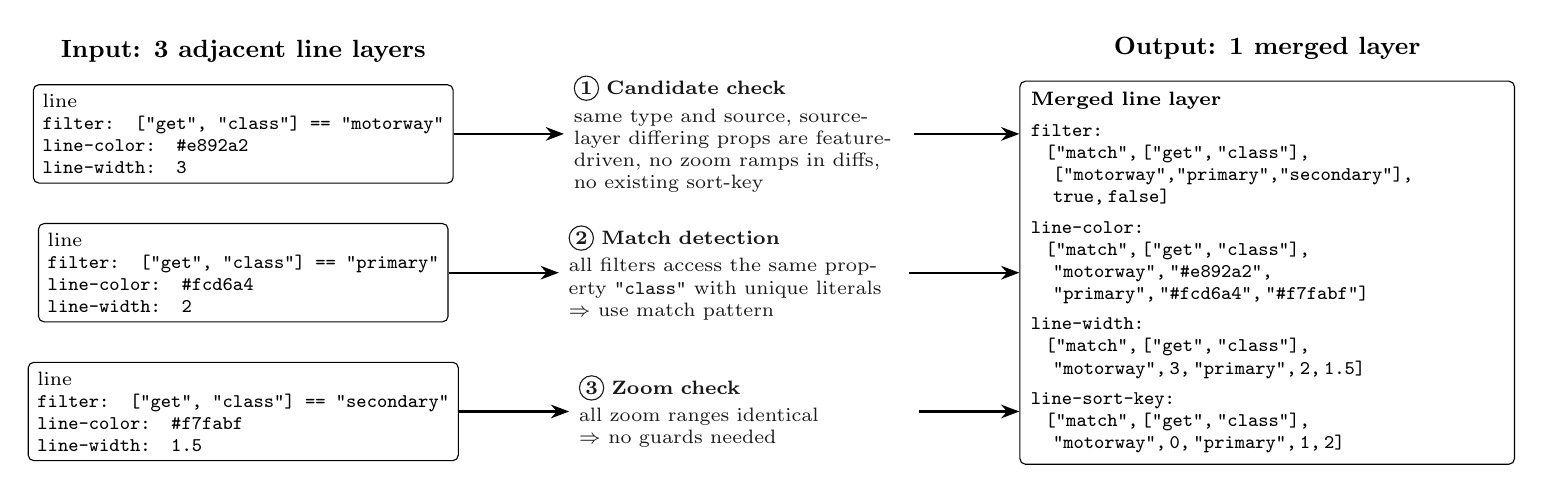
\begin{tikzpicture}[
        node distance=0.35cm,
        layer/.style={rectangle, draw, rounded corners=2pt, minimum width=3.2cm,
                      minimum height=0.55cm, font=\scriptsize, align=left},
        merged/.style={rectangle, draw, rounded corners=2pt, minimum width=4.8cm,
                       font=\scriptsize, align=left, inner sep=4pt},
        phase/.style={rectangle, draw, dashed, rounded corners=3pt, fill=gray!8,
                      inner sep=5pt},
        arrow/.style={-Stealth, thick},
        label/.style={font=\scriptsize\itshape, text=black!90},
        check/.style={font=\scriptsize, text=black!90},
    ]
        % Input layers (left)
        \node[layer]   (l0) {\mlval{line}\\ \texttt{\mlprop{filter}: [\mlop{"get"}, \mlval{"class"}] == \mlval{"motorway"}}\\\texttt{\mlprop{line-color}: \mlval{\#e892a2}}\\\texttt{\mlprop{line-width}: \mlval{3}}};
        \node[layer, below=0.5cm of l0] (l1) {\mlval{line}\\\texttt{\mlprop{filter}: [\mlop{"get"}, \mlval{"class"}] == \mlval{"primary"}}\\\texttt{\mlprop{line-color}: \mlval{\#fcd6a4}}\\\texttt{\mlprop{line-width}: \mlval{2}}};
        \node[layer, below=0.5cm of l1] (l2) {\mlval{line}\\\texttt{\mlprop{filter}: [\mlop{"get"}, \mlval{"class"}] == \mlval{"secondary"}}\\\texttt{\mlprop{line-color}: \mlval{\#f7fabf}}\\\texttt{\mlprop{line-width}: \mlval{1.5}}};

        \node[above=0.15cm of l0, font=\small\bfseries] {Input: 3 adjacent line layers};

        % Phase annotations (middle)
        \node[right=1.4cm of l0, check, text width=4.2cm] (p1) {%
            \stepcirc{1}~\textbf{Candidate check}\\[2pt]
            same type and source,
            source-layer differing props are feature-driven,
            no zoom ramps in diffs,
            no existing sort-key};
        \node[right=1.4cm of l1, check, text width=4.2cm] (p2) {%
            \stepcirc{2}~\textbf{Match detection}\\[2pt]
            all filters access the same property \texttt{\mlval{"class"}} with unique literals\\
            $\Rightarrow$ use \mlop{match} pattern};
        \node[right=1.4cm of l2, check, text width=4.2cm] (p3) {%
            \stepcirc{3}~\textbf{Zoom check}\\[2pt]
            all zoom ranges identical\\
            $\Rightarrow$ no guards needed};

        % Output (right)
        \node[merged, right=1.4cm of p2, text width=6.0cm] (out) {%
            \textbf{Merged \mlval{line} layer}\\[3pt]
            \texttt{\mlprop{filter}:}\\
            \texttt{~~[\mlop{"match"},\,[\mlop{"get"},\,\mlval{"class"}],}\\
            \texttt{~~~[\mlval{"motorway"},\mlval{"primary"},\mlval{"secondary"}],}\\
            \texttt{~~~\mlval{true},\,\mlval{false}]}\\[3pt]
            \texttt{\mlprop{line-color}:}\\
            \texttt{~~[\mlop{"match"},\,[\mlop{"get"},\,\mlval{"class"}],}\\
            \texttt{~~~\mlval{"motorway"},\,\mlval{"\#e892a2"},}\\
            \texttt{~~~\mlval{"primary"},\,\mlval{"\#fcd6a4"},\,\mlval{"\#f7fabf"}]}\\[3pt]
            \texttt{\mlprop{line-width}:}\\
            \texttt{~~[\mlop{"match"},\,[\mlop{"get"},\,\mlval{"class"}],}\\
            \texttt{~~~\mlval{"motorway"},\,\mlval{3},\,\mlval{"primary"},\,\mlval{2},\,\mlval{1.5}]}\\[3pt]
            \texttt{\mlprop{line-sort-key}:}\\
            \texttt{~~[\mlop{"match"},\,[\mlop{"get"},\,\mlval{"class"}],}\\
            \texttt{~~~\mlval{"motorway"},\,\mlval{0},\,\mlval{"primary"},\,\mlval{1},\,\mlval{2}]}
        };

        \node[above=0.15cm of out, font=\small\bfseries] {Output: 1 merged layer};

        % Arrows
        \draw[arrow] (l0.east) -- (p1.west);
        \draw[arrow] (l1.east) -- (p2.west);
        \draw[arrow] (l2.east) -- (p3.west);
        \draw[arrow] (p1.east) -- (out.west |- p1.east);
        \draw[arrow] (p2.east) -- (out.west);
        \draw[arrow] (p3.east) -- (out.west |- p3.east);
    \end{tikzpicture}}
    \caption{
Layer merging example.  Three adjacent line layers differing only in filter literal, color, and width are merged via the \mlop{match} pattern (Phase~2).
    The merged layer uses \texttt{[\mlop{"match"}, [\mlop{"get"}, \mlval{"class"}], \ldots]} for the filter, each differing paint property, and a synthezised sort key that preserves the original draw order.
    Phase~1 validates that all differing properties support feature-driven expressions, and Phase~3 confirms identical zoom ranges, so no zoom guards are needed}
    \label{fig:layer_merge_example}
\end{figure}

\subsection{Data-Level Optimizations}\label{sub:data_optimizations}

Data-level optimizations transform the tile data itself, reducing transfer size and decoding cost without altering the rendered output (constraint to \cref{eq:visual_equivalence}).
The encoding techniques used are surveyed in \cref{sec:data_encoding}.
\cref{tab:data_passes} summarizes the techniques we implemented.

\begin{table}[htbp]
\centering
\begin{tblr}{
  colspec = {p{3.9cm} p{1.8cm} p{9.5cm}},
  rows = {font=\small},
  row{1} = {font=\small\bfseries},
}
\toprule
Pass & Data & Description [compiler analogy] \\
\midrule
Tile shaving             & full scan & Encode only the properties, layers, and geometry types that the style actually references [tree shaking] \\
Transparent re-encoding  & full scan & Re-encode \ac{MVT} tiles into the \ac{MLT} format [instruction set translation] \\
Compression optimizations & full scan & Apply column-aware compression strategies based on data characteristics [\ac{PGO} optimizations] \\
\bottomrule
\end{tblr}
\caption{
Data-level optimization techniques, all requiring a full tile scan.
Together they form a logical, physical, and cost pipeline: tile shaving eliminates unreferenced data, re-encoding transforms the wire format, and compression optimizations select the most compact per-column encoding strategy.}
\label{tab:data_passes}
\end{table}

The pipeline operates in three stages that mirror a database query optimizer's \emph{logical} rewriting, \emph{physical} strategy selection, and \emph{cost-based} competition.

\begin{enumerate}
    \item \textbf{Style-driven tile shaving} (\cref{sub:tile_shaving}): the pipeline analyses the optimized style to produce a \emph{tile pruning advisory} that specifies, per source-layer and zoom level, which properties, geometry types, and property values to retain.
    It then prunes tiles according to this advisory before encoding.
    \item \textbf{Data transformations} (\cref{sub:string_property_interning,sub:feature_reordering}): the pipeline transforms remaining data to improve compressibility, replacing categorical string properties by frequency-ordered integers (\emph{string interning}) and reordering features to exploit spatial or categorical locality.
    \item \textbf{Encoding strategy selection} (\cref{sub:encoding_strategies}): the pipeline re-encodes the pruned, transformed data into \ac{MLT} using a multi-strategy competition that automatically profiles each data stream and selects the most compact encoding.
\end{enumerate}

\noindent The three stages compose:
shaving narrows the column set fed to Stage~2, which in turn determines the value distributions Stage~3 sees.
Stage~3's profiler-driven candidate pruning responds to those distributions $\bar{S}$ automatically.
Its viability tests (rle is considered if $\bar{S}_\text{rle} \geq 2.0$, delta bit-widths beat raw $\bar{S}_\Delta \geq 2.0$) operate on actual stream statistics, so a column whose distinct-value count drops after shaving naturally presents longer runs and triggers more compact candidates.

\paragraph{Style-Driven Tile Shaving}\label{sub:tile_shaving}

The bridge between style-level and data-level optimizations is the \emph{tile pruning advisory}, a structured report that captures, for each source-layer and zoom level, exactly what the rendering style needs.
We compute the advisory from the \emph{optimized} style (after all expression and structural passes) together with tile statistics.
The ordering matters because dead layer elimination, metadata refinement, and layer merging shrink the live-layer set, which in turn reduces the referenced properties and geometry types the advisory carries into the data level.
The empirical character of this style-to-data cascade is taken up in \cref{sub:mlt_results}.
The cascade mirrors the materialized-view maintenance problem, with the rendering style as the view definition, the tile set as the base relation, and the shaved tile as the materialized view.

\noindent The advisory captures the following per source-layer:

\begin{description}
    \item[\textbf{Used properties with zoom ranges}] for each property name appearing in a \texttt{[\mlop{"get"},~\ldots]} or \texttt{[\mlop{"has"},~\ldots]} expression in any live style layer, the zoom range over which it is referenced.
    Properties not referenced at any zoom level are candidates for removal.
    \item[\textbf{Used geometry types with zoom ranges}] which of Point, LineString, and Polygon are needed, derived from the style layer types (e.g., \texttt{\mlval{fill}} $\to$ Polygon, \texttt{\mlval{circle}} $\to$ Point).
    The pass removes features with geometry types unused by any style layer at the current zoom level.
    \item[\textbf{Unused zoom levels}] zoom levels at which no style layer targets the source-layer.
    Tiles at these zoom levels need not be encoded at all.
    \item[\textbf{Unused property values}] specific values of categorical properties that are never matched by any style filter.
    For example, if no style layer allows for a line with a \texttt{class=ferry} property, the pass can remove features with that value.
    \item[\textbf{Feature ID requirement}] whether any style layer uses \texttt{[\mlop{"id"}]} or \texttt{[\mlop{"feature-state"},~\ldots]}.
    When IDs are unused, the pass strips the entire ID column.
\end{description}

\noindent The pipeline applies the pruning advisory to each \ac{MVT} tile before encoding (\cref{fig:tile_shaving_pipeline}).

\begin{figure}[htbp]
    \centering
    \begin{tikzpicture}[
        box/.style={rectangle, draw, rounded corners=2pt, minimum height=0.65cm, font=\small, align=center},
        style/.style={box, fill=roleStyle!20, minimum width=2.8cm},
        data/.style={box, fill=roleData!25, minimum width=2.8cm},
        both/.style={box, fill=roleBoth!20, minimum width=2.8cm},
        arrow/.style={-Stealth, thick},
        lbl/.style={font=\scriptsize\itshape, text=darkgray, align=center},
        steps/.style={rectangle, draw, dashed, rounded corners=2pt, font=\small,
                      align=left, inner sep=6pt, text=black!80},
    ]
        % Row 1: style-side and data-side inputs
        \node[style] (sopt) {Style optimizations\\{\scriptsize (\cref{sub:expression_optimizations,sub:structural_optimizations})}};

        % Row 2: advisory
        \node[both, right=3cm of sopt] (adv) {Tile pruning advisory};
        \draw[arrow] (sopt) -- node[above, lbl] {optimized style} (adv);

        % Row 3:
        \node[data, right=3cm of adv] (stats) {Tile statistics};
        \draw[arrow] (stats) -- node[above, lbl] {property/\\geom distribution} (adv);

        % Row 3: MVT -> prune -> MLT
        \node[data, below=1.0cm of adv] (prune) {Prune \& transform};
        \node[data] at ($(sopt |- prune)$) (mvt) {\ac{MVT} tile};
        \node[data] at ($(stats |- prune)$) (mlt) {\ac{MLT} tile};

        \draw[arrow] (adv) -- (prune);
        \draw[arrow] (mvt) -- (prune);
        \draw[arrow] (prune) -- node[above, lbl] {re-encode} (mlt);

        % Pruning steps annotation
        \node[steps, below=0.5cm of prune] (ops) {%
            \textbf{Pruning operations (in order):}\\[2pt]
            1.\;Remove entire source-layers not referenced by any style layer.\\
            2.\;For each remaining layer:\\
            \quad a.\;Filter features by geometry type at current zoom.\\
            \quad b.\;Filter features by unused categorical property values.\\
            \quad c.\;Strip unused properties from the key-value table.\\
            \quad d.\;Strip feature IDs when not needed.%
        };
        \draw[dashed, gray] (prune) -- (ops);
    \end{tikzpicture}
    \caption{
Style-driven tile shaving pipeline.  The optimized style and tile statistics jointly produce a pruning advisory.  Each \ac{MVT} tile is pruned according to the advisory, transformed, and re-encoded as \ac{MLT}.  Style-level dead layer elimination narrows the advisory, which can reduce the data that must be encoded}
    \label{fig:tile_shaving_pipeline}
\end{figure}

\noindent After pruning, two data transformations improve compressibility before encoding.

\paragraph{String property interning}\label{sub:string_property_interning}
We replace categorical string properties (such as road class, land-use type, or administrative level) by frequency-ordered integer indices.
We derive the interning table from the tile statistics: we sort all distinct values of a string property by descending frequency and assign each value a sequential integer starting from~0.
The most common value receives index~0, the second most common receives~1, and so on.

This transformation has two benefits.
First, it reduces the per-feature storage cost from a variable-length string (with length prefix and dictionary overhead) to a small integer (typically \qtyrange{1}{2}{\byte} as a \ac{VarInt}, see \cref{sub:physical_integer_compressions}).
Second, the frequency ordering means that common values receive small indices, which compress well under \ac{VarInt} and delta encoding.

The optimizer rewrites the corresponding style expressions to reference the integer indices rather than the original string values.
For example, the optimizer rewrites a filter \texttt{[\mlop{"=="}, [\mlop{"get"}, \mlval{"class"}], \mlval{"primary"}]} to \texttt{[\mlop{"=="}, [\mlop{"get"}, \mlval{"class"}], \mlval{0}]} if \texttt{\mlval{"primary"}} is the most frequent value.
This rewriting ensures that the optimized style remains consistent with the transformed tile data.
Because interned tiles encode property values as style-specific integer indices rather than original strings, they are only compatible with the paired optimized style.
Other consumers (debugging tools, alternative renderers) would see opaque integers.
We therefore treat interning as an optional pipeline stage that can be disabled for multi-consumer deployments where tiles must remain self-describing.

\paragraph{Feature reordering}\label{sub:feature_reordering}
The order of features within a tile layer affects the compressibility of every parallel column.
The encoder explores multiple feature orderings (spatial via Hilbert/Morton curve of first vertex, ID-based, and property-based via grouping by a low-cardinality attribute) and retains the ordering that produces the smallest encoded output.
We describe this in detail in \cref{sub:encoding_strategies}.

\subsection{Reencoding data}

The encoder re-encodes the pruned and transformed data into the \ac{MLT} columnar format through a multi-strategy competition over per-column encodings, complemented by dictionary sharing across columns, geometry- and feature-ID-specific encoders, and a round-trip correctness check against the input.

\paragraph{Automatic Encoding Strategy Selection}\label{sub:encoding_strategies}
The re-encoding proceeds in three stages.
First, the encoder converts the row-oriented \ac{MVT} features into an owned columnar representation, with separate arrays for each property column, the geometry vertex buffer, and the feature ID column.
Second, it optionally reorders the columnar data according to the sort strategy competition.
Third, it independently encodes each column using the per-stream encoding competition.
The final wire format consists of three concatenated sections per layer: a header (layer name, tile extent, column count), a metadata section (column types, encoding descriptors), and a data section (the encoded streams).

We reformulate the encoding problem in our encoder as a \emph{multi-strategy competition} inspired by \ac{PGO} in compilers~\cite{changUsingProfileInformation1991} and the instance-optimized systems vision of SageDB~\cite{dingSageDBInstanceOptimizedData2022}:
rather than committing to a single encoding plan, the encoder uses the data distribution of each tile to try multiple strategies, measures the output size of each, and selects the smallest result.

This competition operates at two nested levels.
An \emph{outer loop} that tries multiple feature sort orderings, and an \emph{inner loop} that selects the best integer encoding for each individual data stream.
We deliberately make the inner competition criterion \emph{single-objective} (smallest encoded size).
We do not resolve multi-axis trade-offs (between transfer size, decoding latency, rendering throughput, and preprocessing cost) inside the encoder.
We report them separately per metric in the ablation evaluation (\cref{ch:experiments}), consistent with \cref{sec:problem_statement}: the deployment metrics of \cref{sub:metrics} are characterised per-axis rather than aggregated into a single objective, and the encoder's local size minimisation is a contributing quantity to the load-time axis rather than a global cost function.

A no-copy alternatives mechanism lets each candidate write into the encoder's buffers and rolls losing candidates back by resetting cursor positions, so the inner and outer competitions nest without redundant allocation.
Combined with warm-start caching of \ac{FSST} compressors and vertex-strategy decisions across sort trials, this keeps the cost of the nested competition near-additive rather than multiplicative in the number of trials. \cref{ch:experiments} reports the resulting preprocessing time empirically.
\Cref{fig:arch_enc} summarizes the encoder and decoder data-flow in \texttt{mlt-core}.

\begin{figure}[htbp]
    \centering
    \begin{subfigure}[t]{0.45\linewidth}
        \centering
        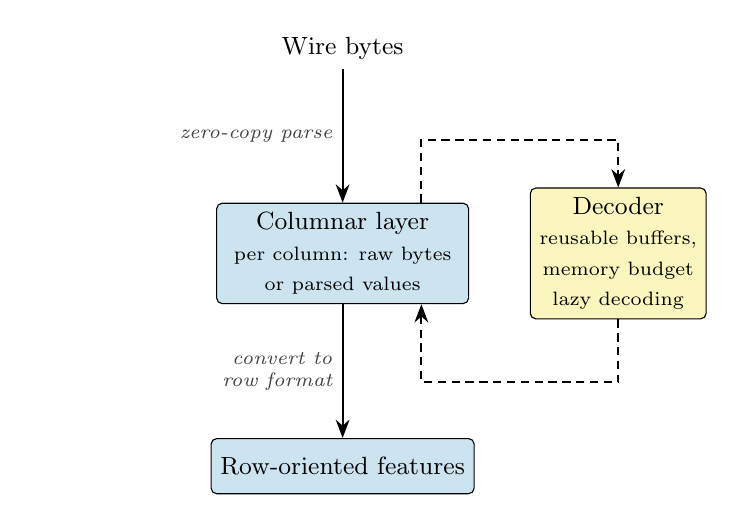
\begin{tikzpicture}[
            box/.style={rectangle, draw, rounded corners=2pt, minimum height=0.7cm,
                        minimum width=2.4cm, font=\small, align=center},
            decode/.style={box, fill=roleSrc!20},
            dec/.style={box, fill=roleOpt!35, minimum width=1.6cm},
            io/.style={font=\small},
            arrow/.style={-Stealth, thick},
            lbl/.style={font=\scriptsize\itshape, text=darkgray},
            node distance=1.7cm,
        ]
            % Main pipeline on centre line (x=0)
            \node[io]     (u8)     {Wire bytes};
            \node[decode, below=of u8, minimum width=3.2cm, align=center]     (name)
                {Columnar layer\\{\scriptsize per column: raw bytes}\\{\scriptsize or parsed values}};
            \draw[arrow] (u8)   -- node[left, lbl, align=right] {zero-copy parse} (name);
            \node[decode, below=of name] (tile)   {Row-oriented features};
            \draw[arrow] (name) -- node[left, lbl, align=right] {convert to\\row format} (tile);

            % Decoder off-centre towards the middle (right side)
            \node[dec, right=3.5cm of name.center, anchor=center] (decnode)
            {Decoder\\{\scriptsize reusable buffers,}\\{\scriptsize memory budget}\\{\scriptsize lazy decoding}};
            \draw[-Stealth, thick, densely dashed]
            ($(name.north) + (1,0)$) -- ++(0,0.8) -| (decnode.north);
            \draw[-Stealth, thick, densely dashed]
            (decnode.south) -- ++(0,-0.8) -| ($(name.south) + (1,0)$);

            % Phantom to balance bounding box
            \path (-4, 0);

            % Decoder arrows
        \end{tikzpicture}
        \caption{
Decoding pipeline.
An input byte slice is zero-copy parsed into a columnar layer whose columns are held lazily as either raw bytes or parsed values, decoded on demand.
The columnar data is converted to row-oriented features as needed.}
        \label{fig:arch_dec_sub}
    \end{subfigure}
    \hfill
    \begin{subfigure}[t]{0.45\linewidth}
        \centering
        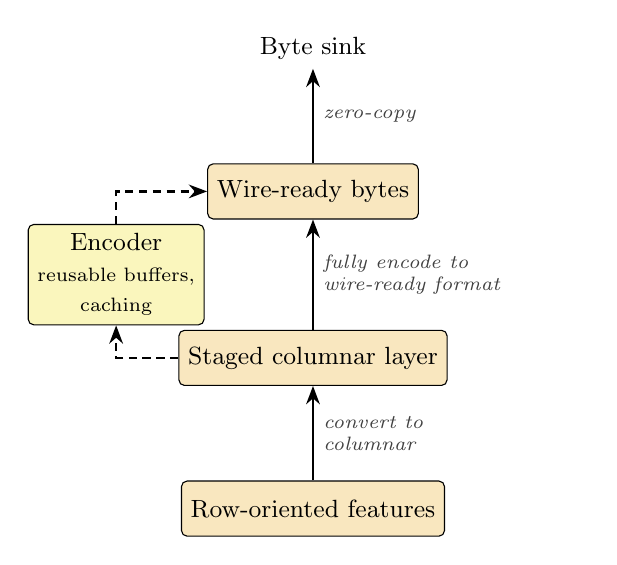
\begin{tikzpicture}[
            box/.style={rectangle, draw, rounded corners=2pt, minimum height=0.7cm,
                        minimum width=2.0cm, font=\small, align=center},
            encode/.style={box, fill=roleData!25},
            enc/.style={box, fill=roleOpt!35, minimum width=1.6cm},
            io/.style={font=\small},
            arrow/.style={-Stealth, thick},
            lbl/.style={font=\scriptsize\itshape, text=darkgray},
            node distance=1.2cm,
        ]
            % Main pipeline on centre line (x=0)
            \node[io]     (write)   {Byte sink};
            \node[encode, below=of write]   (encoded) {Wire-ready bytes};
            \node[encode, below=1.4cm of encoded] (staged)  {Staged columnar layer};
            \node[encode, below=of staged]  (tile)    {Row-oriented features};

            % Encoder off-centre towards the middle (left side)
            \node[enc] at ($(staged)!0.5!(encoded) + (-2.5,0)$) (encnode) {Encoder\\{\scriptsize reusable buffers,}\\{\scriptsize caching}};

            \draw[arrow] (tile)    -- node[right, lbl, align=left] {convert to\\columnar} (staged);
            \draw[arrow] (staged)  -- node[right, lbl, align=left] {fully encode to\\wire-ready format} (encoded);
            \draw[arrow] (encoded) -- node[right, lbl] {zero-copy} (write);

            % Phantom to balance bounding box
            \path (3.5, 0);

            % Encoder arrows
            \draw[-Stealth, thick, densely dashed] (staged.west) -| (encnode.south);
            \draw[-Stealth, thick, densely dashed] (encnode.north) |- (encoded.west);
        \end{tikzpicture}
        \caption{
Encoding pipeline.
Row-oriented features are converted to a staged columnar layer, fully encoded to wire-ready byte buffers by the encoder that implements the multi-strategy competition, and written to a byte sink via a final zero-copy step.}
        \label{fig:arch_enc_sub}
    \end{subfigure}
    \caption{
Encoder~\subref{fig:arch_enc_sub} and decoder~\subref{fig:arch_dec_sub} data-flow in \texttt{mlt-core}}
    \label{fig:arch_enc}
\end{figure}

In an outer loop, the encoder runs a sort-strategy competition.
Reordering features within a layer permutes every parallel column (geometry, IDs, and all properties) simultaneously.
Different orderings favour different encoding schemes.
Spatial orderings cluster nearby geometries and their correlated properties, improving \ac{RLE} run lengths.
ID ordering produces sequential integer sequences amenable to delta-\acs{RLE}.
Which ordering wins depends on the value distributions and cardinalities of the specific layer.
A layer dominated by a single repeated property value may benefit most from spatial clustering, while a layer with sequential IDs and high-cardinality properties may favour ID ordering.
Because this balance shifts across layers, zoom levels, and tilesets, no single ordering dominates universally, and the choice cannot be resolved statically.

The encoder therefore tries multiple sort strategies on the same data and retains the encoding with the smallest total byte count; \cref{fig:sort_competition} diagrams the resulting trial-and-retain loop, including the bounding-box pruning that skips spatial trials for large, widely-spread layers.
The implemented strategies and their rationale are:

\begin{description}
    \item[\textbf{Unsorted}] the encoder preserves the original feature order.
    \item[\textbf{Spatial (Morton/Z-order)}] the encoder sorts features by the Z-order curve index of their first vertex, computed via bit-interleaving.  Fast to compute and provides reasonable spatial locality (\cref{sub:space_filling_curves}).
    \item[\textbf{Spatial (Hilbert)}] the encoder sorts features by the Hilbert curve index of their first vertex.  Slower to compute than Morton but achieves superior spatial locality, as the Hilbert curve avoids the long jumps inherent in the Z-order curve's recursive structure~\cite{moonAnalysisClusteringProperties2001}.
    \item[\textbf{ID}] the encoder sorts features by feature ID in ascending order.
\end{description}

For each candidate strategy, the encoder constructs a fresh \texttt{Encoder} instance, encodes the reordered layer, and measures the total output size (header + metadata + data).
The encoder retains the strategy producing the smallest output and discards all others.
When only a single strategy is applicable, the encoder elides the competition and encodes the layer directly without cloning.
We considered property-based sort strategies but did not include them in the current implementation, because the string interning pass (\cref{sub:string_property_interning}) already groups features of the same discriminator value into dense dictionary-index ranges, and Hilbert or ID ordering strictly dominated an explicit categorical sort on the benchmark tileset.

\begin{figure}[H]
    \centering
    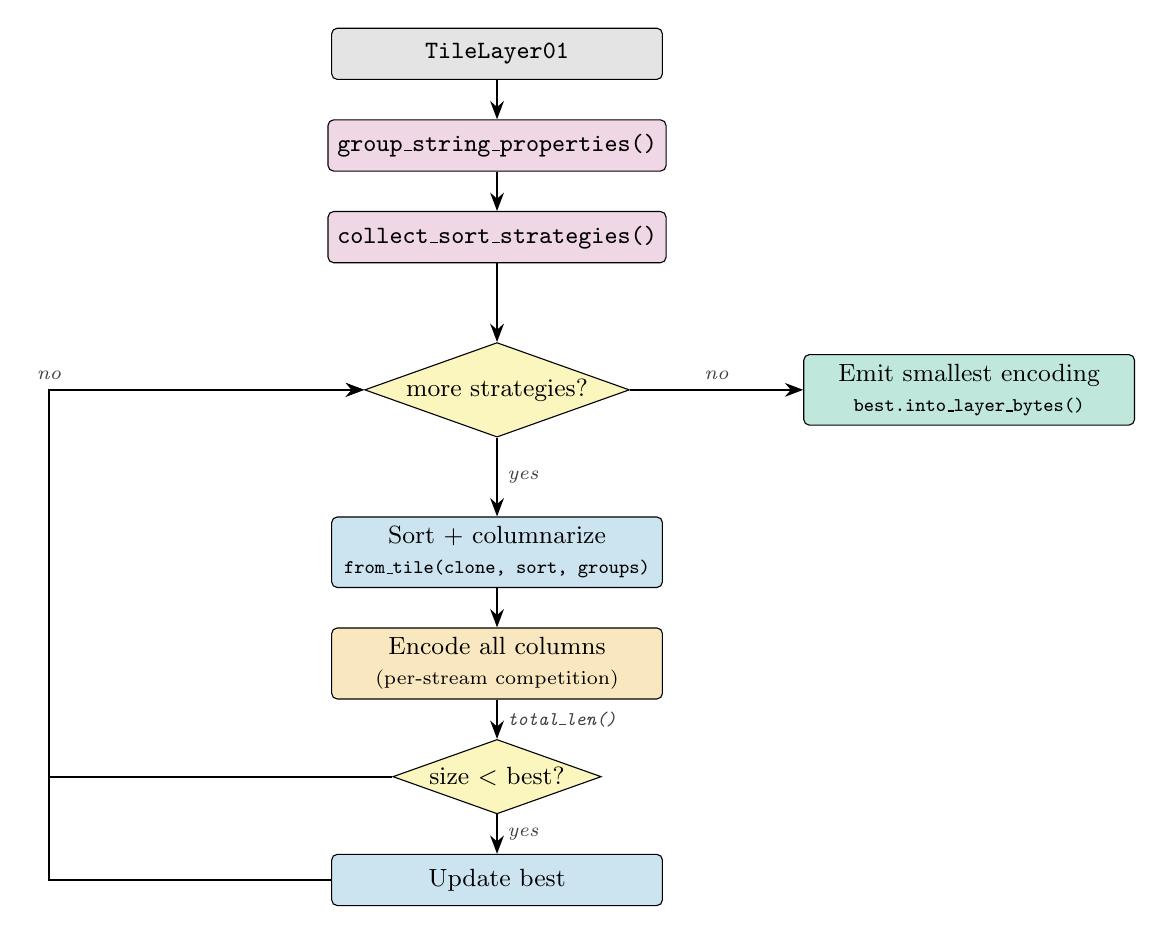
\begin{tikzpicture}[
        node distance=0.5cm,
        box/.style={rectangle, draw, rounded corners=2pt, minimum width=4.2cm,
            minimum height=0.65cm, font=\small, align=center},
        input/.style={box, fill=roleInput!40},
        prep/.style={box, fill=roleMir!30},
        stage/.style={box, fill=roleStyle!20},
        encoder/.style={box, fill=roleData!25},
        decision/.style={diamond, draw, fill=roleDecision!35, aspect=2.8,
            font=\small, inner sep=1pt},
        output/.style={box, fill=roleOutput!25},
        arrow/.style={-Stealth, thick},
        label/.style={font=\scriptsize\itshape, text=darkgray},
        ]
        % Input
        \node[input] (layer) {\texttt{TileLayer01}};

        % Prep: group_string_properties
        \node[prep, below=of layer] (grp)
        {\texttt{group\_string\_properties()}};
        \draw[arrow] (layer) -- (grp);

        % Prep: collect_sort_strategies
        \node[prep, below=of grp] (coll)
        {\texttt{collect\_sort\_strategies()}};
        \draw[arrow] (grp) -- (coll);

        % Loop guard
        \node[decision, below=1.0cm of coll] (more) {more strategies?};
        \draw[arrow] (coll) -- (more);

        % Sort + columnarize
        \node[stage, below=1.0cm of more] (sort)
        {Sort + columnarize\\%
            {\scriptsize\texttt{from\_tile(clone, sort, groups)}}};
        \draw[arrow] (more) -- node[right, label] {yes} (sort);

        % Encode
        \node[encoder, below=of sort] (enc)
        {Encode all columns\\{\scriptsize (per-stream competition)}};
        \draw[arrow] (sort) -- (enc);

        % Compare
        \node[decision, below=of enc] (cmp) {size $<$ best?};
        \draw[arrow] (enc) -- node[right, label] {\texttt{total\_len()}} (cmp);

        % Yes: update best, then loop back
        \node[stage, below=0.5cm of cmp] (upd) {Update best};
        \draw[arrow] (cmp) -- node[right, label] {yes} (upd);

        % No: discard, loop back
        \draw[arrow] (upd.west) -| ($(more.west)+(-4cm,0)$) |- node[above, label] {no} (more.west);
        \draw[arrow] (cmp.west) -| ($(more.west)+(-4cm,0)$) |- (more.west);

        % Exit loop
        \node[output, right=2.2cm of more] (best) {Emit smallest encoding\\{\scriptsize\texttt{best.into\_layer\_bytes()}}};
        \draw[arrow] (more.east) -- node[above, label] {no} (best.west);
    \end{tikzpicture}
    \caption{
Multi-strategy sort competition.
        Shared-dictionary string groups are computed once and reused across all trials.
        The encoder collects candidate sort strategies, pruning spatial strategies via the bounding-box heuristic for large, widely-spread layers.
        For each candidate, the layer is cloned, sorted, and columnarized via \texttt{from\_tile}.
The columnar data is then encoded with per-stream integer competitions.
        The encoding with the smallest \texttt{total\_len()} is retained}
    \label{fig:sort_competition}
\end{figure}

To avoid wasting trials on unpromising strategies, a \emph{bounding-box heuristic} skips spatial sorting on large layers whose features are too spatially dispersed for locality clustering to help.
Specifically, for layers with more than \texttt{512} features, the heuristic prunes spatial trials when the first-vertex bounding box covers more than \texttt{80\%} of the tile extent on \emph{both} axes.
The encoder always tries small layers (below the threshold), since the absolute cost of an extra encoding pass is negligible for them.
We derived the thresholds experimentally from Germany-wide OpenMapTiles.

In an inner loop, a per-stream encoding competition tries every viable integer encoding for the data stream.
Each candidate pairs a \emph{logical} encoding (Plain, Delta, \ac{RLE}, or DeltaRle) with a \emph{physical} encoding (\ac{VarInt} or \ac{FastPFOR}~\cite{lemireDecodingBillionsIntegers2015}).
The general stream competition currently covers these four logical encodings.
The encoder applies geometry-specific strategies (Morton-delta, componentwise-delta) via a separate encoding path optimized for coordinate data, since their semantics are tied to the two-dimensional structure of vertex sequences and do not generalize to property columns.
Extending the general competition to include additional strategies (e.g., frame-of-reference without delta, or hybrid schemes) is a direction for future work, though the current candidate set captures the dominant encoding patterns observed in the benchmark tileset.
The naive approach of encoding every combination and comparing would be prohibitively expensive for large tiles.
Instead, a \emph{data profiler} samples a contiguous block taken from the middle of the stream: it profiles streams with at most $512$ values in full, and profiles longer streams over $\lfloor |s| / 100 \rfloor$ values clamped to $[512,\, 16384]$.
We chose the contiguous mid-stream window over a random sample because permutation destroys \ac{RLE} run lengths and delta-bit-width statistics, and because the middle of a spatially or ID-sorted stream is a representative point away from the boundary artefacts at the ends.
The profiler completes a single pass over the sample to prune candidates before any full encoding is attempted.
It excludes \ac{RLE} when the average run length $\bar{S} = |s| / n_{\text{runs}}$ falls below 2.0.
It excludes Delta when the stream is non-monotonic and the summed bit width of the zigzag-encoded deltas exceeds that of the raw values.
It excludes DeltaRle when the delta-stream average run length $\bar{S}_\Delta = (|s|-1) / n_{\Delta\text{-runs}}$ falls below 2.0 and neither \ac{RLE} nor Delta is independently viable.
The encoder only offers \ac{FastPFOR} for 32-bit integer types, as the algorithm's block structure is designed for fixed-width words.
The encoder fully encodes the remaining candidates (typically two to four) and commits the smallest output.

\paragraph{String encoding}
String columns compete across four strategies, reflecting the two orthogonal dimensions of string compression: deduplication and byte-level compression.

\begin{description}
    \item[\textbf{Plain}] raw bytes with length prefixes.
    The length stream is itself subject to the integer encoding competition.
    \item[\textbf{Dictionary}] a deduplicated corpus with per-string offset indices.
    Effective when many features share the same string value (e.g., road names that repeat across tiles).
    \item[\textbf{\ac{FSST}} (\cref{sub:string_compression})]~\cite{bonczFSSTFastRandom2020}
    A lightweight, random-access string compressor that learns a symbol table of up to~255 frequent byte sequences and replaces occurrences with single-byte codes.
    The encoder stores the symbol table once per column.
The compressed corpus remains directly scannable without decompression.
    \item[\textbf{\ac{FSST} + Dictionary}] \ac{FSST} applied to a deduplicated dictionary, combining both deduplication and byte-level compression.
\end{description}

A viability probe ensures that the encoder only attempts \ac{FSST} when the symbol-table overhead (up to \qty{2040}{\byte}) is likely to be recouped: it excludes columns below \num{2048}~raw bytes and evaluates a trial compression on a sample of up to \num{256} strings before committing.
The encoder caches trained \ac{FSST} compressors by column name and reuses them across all sort-strategy trials, avoiding redundant training.
The encoder applies a novel \emph{pruning variant} of \ac{FSST} that drops symbols from the persisted table when inlining their occurrences as escaped literals costs fewer bytes than retaining the table entry, shrinking the symbol table without changing the decoder.

\paragraph{Shared dictionary grouping}\label{sub:cardinality}
The \ac{MLT} format supports shared dictionaries where multiple string columns reference a common deduplicated corpus, amortising dictionary overhead across columns with overlapping vocabularies.
The reference encoder groups columns by naming prefix (e.g., \texttt{\mlval{name}}, \texttt{\mlval{name:en}}, \texttt{\mlval{name:de}}), which misses semantic overlaps (e.g., \texttt{\mlval{class}} and \texttt{\mlval{subclass}} in OpenMapTiles share many values).

\begin{sloppypar}
    Our encoder replaces prefix matching with MinHash-based similarity clustering (\cref{sub:lsh})~\cite{broderResemblanceContainmentDocuments1998}.
    \Cref{fig:minhash_clustering} walks through the four-step pipeline from per-column vocabularies through MinHash signatures and pairwise Jaccard estimation to the final Union-Find clustering.
    For each string column, the encoder computes two MinHash sketches of $128$ permutations: one over exact string values and one over byte trigrams (3-byte sliding windows).
    The choice of 128 permutations corresponds to an expected standard error of approximately $1/\sqrt{128} \approx 8.8\%$ on the Jaccard estimate, which is adequate for the binary accept/reject decision of the clustering step.
    The trigram sketch captures partial overlap between columns whose values are substrings or morphological variants of each other.
    The encoder estimates pairwise Jaccard similarity as $\hat{J} = |\{i : h_i^{(a)} = h_i^{(b)}\}| / 128$ for each sketch type and takes the maximum of two estimates.
    The encoder unifies columns whose similarity exceeds \texttt{7.5\%} via a Union-Find structure (union by size).
The low threshold reflects that even small vocabulary overlap reduces the marginal cost of adding a column to an existing dictionary.
    The encoder discards groups with fewer than two members.
    We selected the threshold and similarity mode via a sweep over $[2.5\%, 20\%]$ on the Germany OpenMapTiles tileset under three similarity modes (\emph{hybrid} taking $\max(\hat{J}_\text{exact}, \hat{J}_\text{trigram})$, \emph{only-trigram}, \emph{only-exact}), summarised in \cref{fig:minhash_sweep} in the appendix.
    Hybrid mode wins at every threshold at no significant performance cost, and the curve is nearly flat below \qty{7.5}{\percent}, where the empirical optimum at \qty{2.5}{\percent} saves only an additional \qty{1.6}{\mega\byte} on the \qty{3.14}{\giga\byte} tileset at the cost of false-positive union risk on tilesets with less correlated vocabularies.
    We therefore retain \qty{7.5}{\percent} as a conservative default that captures the majority of the grouping benefit.
\end{sloppypar}

\DeclareRobustCommand{\circled}[1]{\tikz[baseline=(char.base)]{\node[circle, draw, inner sep=1pt, font=\scriptsize\bfseries] (char) {#1};}}

\begin{figure}[htbp]
    \centering
    \resizebox{\textwidth}{!}{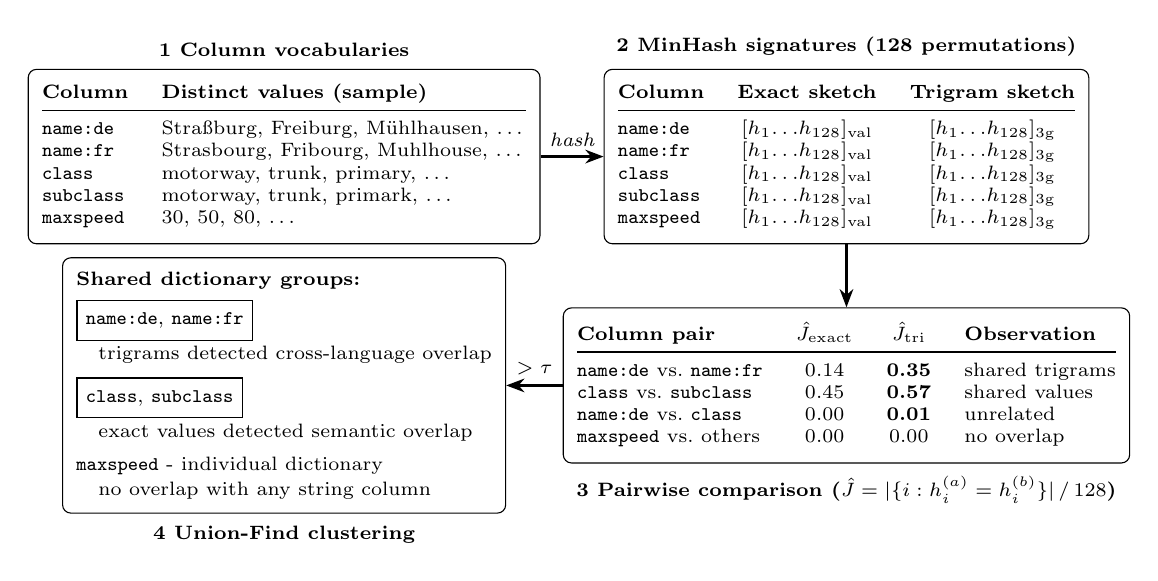
\begin{tikzpicture}[
            arrow/.style={-Stealth, thick},
            cmp/.style={font=\scriptsize, align=left},
            stepbox/.style={draw, rounded corners=3pt, inner sep=5pt, font=\scriptsize},
            steplabel/.style={font=\scriptsize\bfseries},
            ]
            % Top-left (Step 1): Column value table
            \node[stepbox] (tbl) {%
                \begin{tabular}{@{}l l@{}}
                    \textbf{Column} & \textbf{Distinct values (sample)} \\
                    \midrule
                    \texttt{\mlval{name:de}}  & Straßburg, Freiburg, Mühlhausen, \ldots \\
                    \texttt{\mlval{name:fr}}  & Strasbourg, Fribourg, Muhlhouse, \ldots \\
                    \texttt{\mlval{class}}    & motorway, trunk, primary, \ldots \\
                    \texttt{\mlval{subclass}} & motorway, trunk, primark, \ldots \\
                    \texttt{\mlval{maxspeed}} & 30, 50, 80, \ldots
                \end{tabular}%
            };
            \node[steplabel, above=1pt of tbl] {\circled{1} Column vocabularies};

            % Top-right (Step 2): MinHash sketch generation
            \node[stepbox, right=0.8cm of tbl, anchor=west] (hash) {%
                \begin{tabular}{@{}l c c@{}}
                    \textbf{Column} & \textbf{Exact sketch} & \textbf{Trigram sketch} \\
                    \midrule
                    \texttt{\mlval{name:de}}  & $[h_1\!\ldots\!h_{128}]_{\text{val}}$ & $[h_1\!\ldots\!h_{128}]_{\text{3g}}$ \\
                    \texttt{\mlval{name:fr}}  & $[h_1\!\ldots\!h_{128}]_{\text{val}}$ & $[h_1\!\ldots\!h_{128}]_{\text{3g}}$ \\
                    \texttt{\mlval{class}}    & $[h_1\!\ldots\!h_{128}]_{\text{val}}$ & $[h_1\!\ldots\!h_{128}]_{\text{3g}}$ \\
                    \texttt{\mlval{subclass}} & $[h_1\!\ldots\!h_{128}]_{\text{val}}$ & $[h_1\!\ldots\!h_{128}]_{\text{3g}}$ \\
                    \texttt{\mlval{maxspeed}} & $[h_1\!\ldots\!h_{128}]_{\text{val}}$ & $[h_1\!\ldots\!h_{128}]_{\text{3g}}$ \\
                \end{tabular}%
            };
            \node[steplabel, above=1pt of hash] {\circled{2} MinHash signatures (128 permutations)};

            % Bottom-right (Step 3): Pairwise Jaccard
            \node[stepbox, anchor=north] (sim) at ($(hash.south)+(0,-0.8cm)$) {%
            	\begin{tabular}{@{}l c c l@{}}
            		\textbf{Column pair} &
            		$\hat{J}_{\text{exact}}$ &
            		$\hat{J}_{\text{tri}}$ &
            		\textbf{Observation} \\
            		\midrule
            		\texttt{\mlval{name:de}} vs.\ \texttt{\mlval{name:fr}}
            		& 0.14 & \textbf{0.35}
            		& shared trigrams\\

            		\texttt{\mlval{class}} vs.\ \texttt{\mlval{subclass}}
            		& 0.45 & \textbf{0.57}
            		& shared values \\

            		\texttt{\mlval{name:de}} vs.\ \texttt{\mlval{class}}
            		& 0.00 & \textbf{0.01}
            		& unrelated \\

            		\texttt{\mlval{maxspeed}} vs.\ others
            		& 0.00 & 0.00
            		& no overlap \\
            	\end{tabular}%
            };
            \node[steplabel, below=1pt of sim] {\circled{3} Pairwise comparison ($\hat{J} = |\{i : h_i^{(a)} = h_i^{(b)}\}| \,/\, 128$)};

            % Bottom-left (Step 4): Union-Find result
            \node[stepbox, cmp] at ($(tbl |- sim)$)  (res) {%
                \textbf{Shared dictionary groups:}\\[3pt]
                \fbox{\strut\texttt{\mlval{name:de}}, \texttt{\mlval{name:fr}}}\\[1pt]
                \quad{\scriptsize trigrams detected cross-language overlap}\\[4pt]
                \fbox{\strut\texttt{\mlval{class}}, \texttt{\mlval{subclass}}}\\[1pt]
                \quad{\scriptsize exact values detected semantic overlap}\\[4pt]
                \texttt{\mlval{maxspeed}} - individual dictionary\\[1pt]
                \quad{\scriptsize no overlap with any string column}%
            };
            \node[steplabel, below=1pt of res] {\circled{4} Union-Find clustering};

            % Arrows (clockwise)
            \draw[arrow] (tbl) -- node[above, font=\scriptsize\itshape] {hash} (hash);
            \draw[arrow] (hash) -- (sim);
            \draw[arrow] (sim) -- node[above, font=\scriptsize\itshape] {$>\tau$} (res);

    \end{tikzpicture}}
    \caption{
MinHash-based shared dictionary clustering (clockwise from top-left).
        \circled{1}~Each string column's distinct values form a set.
        \circled{2}~Two 128-permutation MinHash sketches are computed per column: one over exact string values, one over byte trigrams (3-byte sliding windows).
        \circled{3}~Pairwise Jaccard similarity is estimated by counting matching hash positions.
The maximum of the two sketch types is compared against threshold $\tau = 0.075$.
        Exact matching detects columns that share literal values (\texttt{\mlval{class}}/ \texttt{\mlval{subclass}}).
Trigram matching detects cross-language morphological variants (\texttt{\mlval{name:de}}/ \texttt{\mlval{name:fr}} in a border region).
        \circled{4}~Column pairs exceeding the threshold are unified via Union-Find.
The resulting groups share a single deduplicated dictionary corpus}
    \label{fig:minhash_clustering}
\end{figure}

\paragraph{Geometry encoding}
The encoder encodes geometry vertices as either \emph{componentwise deltas} (CWD), \emph{Hilbert-code dictionaries}, \emph{Morton-code dictionaries} or plain vertices.
CWD encodes each vertex as the delta from the previous vertex, producing a single interleaved stream $[x_0, y_0, \Delta x_1, \Delta y_1, \ldots]$ that is then compressed via the per-stream integer competition.
The Morton/Hilbert-code dictionary approach computes a Z-order code for each unique vertex pair, stores the deduplicated codes as a sorted dictionary, and references them via per-vertex offset indices, producing two streams (offsets and dictionary deltas) instead of one.
The encoder tries both strategies (when the coordinate range permits Morton encoding, i.e., both axes fit within 16~bits after shifting) and retains the smaller result.


\paragraph{Feature IDs encoding}
The encoder encodes feature IDs through the same per-stream integer competition as other integer columns, with an explicit tag selecting between 32-bit and 64-bit word widths.
The encoder narrows 64-bit-declared ID columns to 32 bits when every observed value fits.

The same data profiler that drives the inner competition discovers structural patterns.
Sequential IDs reach DeltaRle, constant IDs reach \ac{RLE}, and short or irregular sequences fall back to plain \ac{VarInt}.

\paragraph{Encoder correctness validation}\label{par:encoder_validation}
Because \ac{FastPFOR} disclaims input validation and the encoder's narrowing, run-encoding, and dictionary rebuild stages have independent failure modes, we validate correctness through property-based round-trips per integer encoder, coverage-guided fuzzing over full layer round-trips, snapshot tests over the profiler's candidate selection, and the pixel-exact end-to-end check from \cref{sec:visual_correctness}.
This soft-correctness guarantee underwrites the experimental results in \cref{ch:experiments}.

\subsection{Tile Statistics Collection}\label{sub:tile_statistics}

Several optimizations passes require knowledge of the actual tile data, namely stats-driven constant folding and selectivity reordering (\cref{sub:expression_optimizations}), dead elimination with geometry-type mismatch and metadata refinement (\cref{sub:structural_optimizations}), and the tile pruning advisory (\cref{sub:tile_shaving}).
A statistics collection phase provides this knowledge by scanning the tile set and producing a per-source, per-source-layer statistical profile.
The optimizer accepts either an MBTiles database, in which case the scan runs on demand, or a pre-computed statistics file produced by an earlier scan.

For each source layer, the phase collects the following statistics:

\begin{description}
    \item[\textbf{Feature count}] total number of features across all tiles\footnote{Contrairy to na"ive reasoning, eatures appearing in multiple tiles at different zoom levels are counted multipe times, as the optimizer reasons per-tile, not per-geographic-entity.
This creates bias, but bias that is representative to the usecase of rendering maps, where tiled features are used instead of geographic features.}.
    \item[\textbf{Features by zoom}] a per-zoom-level feature count, used by metadata refinement to determine the first and last zoom level at which data exists.
    \item[\textbf{Geometry types}] counts of Point, LineString, and Polygon features, used by dead elimination to detect geometry-type mismatches.
    \item[\textbf{Feature ID presence}] whether any feature carries a non-zero feature ID, used by the advisory to decide whether to strip the ID column.
    \item[\textbf{Per-property statistics}] for each property name, the statistics depend on the wire type:
    \begin{description}
        \item[\emph{Boolean}] present count and true count.
        \item[\emph{Integer/unsigned integer}] present count, minimum, maximum, cardinality, and (if cardinality $\leq 200$) a full value-frequency map.
        \item[\emph{Double}] present count, minimum, maximum, cardinality (no value-frequency map, since floating-point equality is unreliable for folding).
        \item[\emph{String}] present count, cardinality, and (if cardinality $\leq 200$) a value-frequency map sorted by descending frequency.
    \end{description}
\end{description}

We allow collecting statistics at a configurable \emph{sample rate}.
A sample rate of~1.0 (full census) is required for irreversible decisions such as dead layer elimination or property interning.
Lower sample rates are sufficient for selectivity estimation and reordering.
A sample-rate guard in the optimizer enforces this distinction.
Passes that permanently remove data check that the sample rate is~1.0 before applying.

\subsection{Preprocessing Cost Model}\label{sub:preprocessing_cost_model}

All optimizations described above run \emph{offline}, paid once per (style, tileset) build and amortised across every subsequent tile request and rendering session.
The total preprocessing cost decomposes into four additive terms covering style passes (\cref{sub:expression_optimizations,sub:structural_optimizations}), tile statistics (\cref{sub:tile_statistics}), advisory computation (\cref{sub:tile_shaving}), and \ac{MLT} re-encoding (\cref{sub:encoding_strategies}).
\begin{equation}\label{eq:cost_model}
    C_\text{total}(S, T) \;=\; C_\text{style}(S) \;+\; C_\text{stats}(T) \;+\; C_\text{adv}(S) \;+\; C_\text{enc}(S, T).
\end{equation}
Bounding-box pruning, data profiling, \ac{FSST} warm-start caching, scratch-buffer recycling, and the \ac{RAII} alternatives guard together keep $C_\text{enc}$ bounded under the multi-strategy competition.
We report wall-clock cost on the Germany OpenMapTiles tileset in \cref{sub:preprocessing_cost}.
The focus of this thesis is on the delivery and rendering improvements that this one-off cost buys.

\section{Gathering a Representative Sample}\label{sec:gathering_sample}

Our deep evaluation runs 15 styles (\cref{sub:deep_corpus}) against reproducible tile data (\cref{sub:tile_data}) and a stratified scenario sample (\cref{sub:scenarios}).
A further 13 styles (\cref{sub:generalization_corpus}) carry static-only checks to test whether gains generalise beyond the deep tier.

\subsection{Benchmarking Corpus}\label{sub:deep_corpus}

We curated a corpus of 15 publicly available styles that use the OpenMapTiles or BasemapDE schema:
four \textbf{OpenFreeMap} styles (liberty, bright, positron, fiord);
seven \textbf{OpenMapTiles community} styles (dark-matter, osm-bright, klokan-basic, toner, osm-liberty, americana, stadia-outdoors);
and four \textbf{government and institutional} styles (ICGC~fosc, ICGC~gris, Basemap\-DE\footnote{\url{https://basemap.de/}, last accessed 2026-05-23} topo\-graphic, Basemap\-DE color).

These styles span a range of complexity-from minimal basemaps with fewer than 50~layers to verbose institutional styles with several hundred layers-and exercise different subsets of the expression language.

\subsection{Generalisation Corpus}\label{sub:generalization_corpus}

To assess whether optimizations gains generalize beyond the deep corpus, we collected 13 styles from the Maputnik style editor catalog (two additional catalog entries were unavailable at the time of measurement).
These styles are evaluated using static analysis only (style size, complexity metrics, pass applicability) and do not require tile data.

\subsection{Tile Data and Caching}\label{sub:tile_data}

We source tile data from \ac{OSM} via Planetiler or the German government.
We consume both sources through the standard Web Mercator XYZ tiling scheme used by MapLibre, so all zoom-level reasoning in the thesis assumes this grid.
We access BasemapDE through its XYZ-compatible endpoint rather than its native \acs{WMTS}~\cite{masoOpenGISWebMap2010} grid, ensuring that the optimizer's tile indexing is uniform across the corpus.
Only for \ac{OSM} is the underlying data fully available, so only for this source can we collect tile statistics at a sample rate of~1.0.
To ensure reproducibility across benchmark runs, we route all tile requests through a local caching proxy that stores tiles on first access and replays them on subsequent runs with the latency and download speed of a 4G internet connection according to Rusan et al.~\cite{rusanAssessmentPacketLatency2015} ($\frac{\text{size}}{30\,\mathrm{MiB/s}} + 25ms$).
This eliminates network variability and guarantees that every ablation step operates on identical tile data (after an initial, discarded run).
The model does not simulate packet loss, HTTP/2 multiplexing, TCP slow-start, or HTTP/3 (QUIC) with its 0-RTT connection resumption and absence of head-of-line blocking.
All of these would amplify the benefit of smaller tiles, so the measured load-time improvements from tile shaving are a conservative lower bound on what a real deployment would observe.
This ensures that we measure tile-fetch improvements (e.g.\ smaller tiles due to shaving) under conditions representative of a \ac{CDN}-served deployment while remaining deterministic across runs.
The same network model also feeds the per-style \ac{CDN} break-even analysis in \cref{sub:mlt_discussion}, which extends this single-client setup to a multi-style cache.

\subsection{Geographic and Use-Case Scenarios}\label{sub:scenarios}

The benchmark harness defines 18 scenarios drawn from a matrix of 15 geographic locations and 5 camera animation types.
\textbf{locations} span high-density cities with Latin scripts (Munich, Berlin, Paris, New York, Rome), cities with non-Latin scripts (Tokyo, Beijing, Seoul, Cairo), and low-density or special nature regions (Black Forest, Amazon, Swiss Alps, Sahara, Venice, Stockholm Archipelago).
\textbf{animations} exercise different rendering workloads:
\emph{zigzag} alternates zoom levels while panning;
\emph{spiral} traces a circle at constant zoom with rotating bearing;
\emph{zoomdrill} zooms from overview to street level and back;
\emph{pansweep} sweeps across a region at constant zoom;
and \emph{bearingspin} rotates bearing at high pitch.
See \cref{app:animation_patterns} for the keyframe diagrams.

Each scenario is a specific (location, animation) pair.
The full cross-product of 15 locations and 5 animations is 75 pairs, which is too expensive\footnote{Each cell requires 15 repeat runs for statistical validity across 19 ablation steps and 15 styles, as this would result in $75 \times 15 \times 19 \times 15 = \num{320625}$ full animations} to run for every ablation step.
We chose the 18 selected scenarios by stratified sampling so that every location appears at least once and every animation appears at least three times, and so that all combinations of density class (high/low) and script class (Latin/non-Latin) are represented.
Within each stratum we selected the specific (location, animation) pair that exercises the most layers in the densest style in the corpus, ensuring that the sample is biased \emph{against} the null hypothesis of \enquote{no effect}, i.e.\ towards scenarios where any rendering-cost differences are most likely to be visible.

This is a convenience sample by design:
we do not claim it is unbiased across all real-world usage patterns, but we claim it is a reasonable stress test of the optimizer across the dimensions (density, script, zoom trajectory, camera motion) that most plausibly interact with style and data-level optimizations.

\section{Evaluation}\label{sec:evaluation}

Since many of the investigated optimizations techniques have not previously been studied in the context of map rendering pipelines, we must evaluate their effectiveness empirically.
We carry out this empirical evaluation in \cref{ch:experiments}.
The rest of this section defines the methodology that chapter applies.
Our evaluation reports the deployment metrics framed in \cref{sec:problem_statement} along several axes: data savings (which feed the load-time axis), rendering performance, optimization cost (the $C_\text{total}$ breakdown of \cref{sub:preprocessing_cost_model}), and qualitative efficiency.

\begin{description}
    \item[\textbf{Data savings}] reduction in style size (raw, gzip, and Brotli) and tile transfer volume.
    \item[\textbf{Rendering performance}] client-side metrics including load time, frames per second, frame time percentiles (p50, p95, p99), jank count, style parse time, time to first tile, and time to first frame.
    \item[\textbf{Optimization cost}] preprocessing time introduced by each pass, measured as wall-clock time on the optimizer's host machine.
This is an offline cost amortised over all subsequent tile deliveries.
    \item[\textbf{Efficiency}] \emph{qualitative} discussion of the energy implications of reduced data transfer and fewer rendering operations.  We perform no direct power or energy measurement (\ac{RAPL}, battery delta), because the benchmark harness runs on a desktop workstation rather than a thermaly and battery-constrained mobile device.
Any quantitative energy claim would require a different hardware platform and we defer it to future work.
\end{description}

\subsection{Metrics}\label{sub:metrics}

Per run, the benchmark harness collects the following metrics:

\begin{description}
    \item[\textbf{Load time}] wall-clock time from requesting the map to completion of the initial render, including style parsing, tile fetching, tile decoding, and first paint.
    Within the rendering benchmark, decoding latency is embedded in \texttt{loadMs} rather than isolated, because the browser-based harness cannot separate decoder wall-clock time from the surrounding fetch and first-paint work without renderer-internal instrumentation.
    We instead measure isolated decoding throughput via Criterion\footnote{\url{https://github.com/bheisler/criterion.rs}, last accessed 2026-05-23} micro-benchmarks on our decoder (\cref{tab:decode_throughput}).
    \item[\textbf{Style parse time}] time spent parsing and compiling the style \ac{JSON} into the renderer's internal representation.
    \item[\textbf{Time to first tile} (\texttt{firstTileMs})] time from map initialisation until the first tile is decoded and ready for rendering.
    \item[\textbf{Time to first frame}] time until the first frame is composited and presented.
    \item[\textbf{Frames per second} (\texttt{fps})] average rendering throughput during the animation phase.
    \item[\textbf{Frame time percentiles} (\texttt{p50}, \texttt{p95})] distribution of per-frame render times, capturing both typical and worst-case latency.
    \item[\textbf{Jank count}] number of frames exceeding \qty{16.67}{\milli\second} (the 60\,\ac{FPS} budget), indicating visible stuttering.
    \item[\textbf{Heap memory}] JavaScript heap usage during the benchmark, capturing the memory cost of style structures and tile data.
    \item[\textbf{Idle time}] time the renderer spends idle (waiting for tiles or \ac{GPU} sync), indicating headroom.
\end{description}

\noindent Additionally, we compute static metrics for each optimized style without running the renderer.
\textbf{Style size} covers raw byte count, gzip-compressed size, and Brotli-compressed size.
\textbf{Complexity metrics} comprise total \ac{AST} node count, maximum expression depth, layer count, filter count, and expression operator histogram.

\subsection{Ablation Methodology}\label{sub:ablation}

Our primary evaluation methodology is cumulative ablation: we add passes one at a time in a fixed order and re-run the full benchmark suite after each addition.
This reveals both the marginal contribution of each pass and the interactions between passes.
The ablation comprises 19~cumulative steps (a baseline with no optimizations followed by passes added incrementally in the order listed in \crefrange{tab:expression_passes}{tab:data_passes}) plus one additional configuration that applies plain tile shaving on top of the unoptimized style, included to isolate the style$\leftrightarrow$shaving interaction in \cref{sub:mlt_results}.
\cref{sub:combined_ablation,tab:marginal_contribution} present the step-by-step results.

We execute each scenario/style combination for 15~runs.
We report the median and standard deviation of each metric.
We prefer the median over the mean because rendering performance distributions are right-skewed (occasional long frames inflate the mean).
To reduce measurement noise, the benchmark harness pins rendering to real \ac{GPU} hardware via ANGLE\footnote{\url{https://github.com/google/angle}, last accessed 2026-05-23}/Vulkan\footnote{\url{https://www.vulkan.org/}, last accessed 2026-05-23} rather than the software rasteriser used for pixel-exact render tests.
This ensures that we measure \ac{GPU}-bound workloads (fragment shading, texture sampling, blend operations) realistically.

We serve all tile requests from a local caching proxy as described in \cref{sub:tile_data}.
The benchmark harness itself is a Puppeteer\footnote{\url{https://pptr.dev/}, last accessed 2026-05-23}-driven headless browser that programmatically loads the MapLibre GL~JS renderer, applies a camera animation scenario, and collects performance counters via the \texttt{Performance} \ac{API}\footnote{\url{https://developer.mozilla.org/en-US/docs/Web/API/Performance_API}, last accessed 2026-05-23} and custom instrumentation hooks in the renderer.

\begin{chaptersummary}
The optimizer is a \textbf{three-level pipeline} (\cref{sub:pipeline}) operating on the $(S, T) \to (S', T')$ problem of \cref{sec:problem_statement}: eight expression-level passes run to a fixpoint, six structural passes act on a typed style document, and data-level passes re-encode shaved tiles into \ac{MLT} via per-stream strategy competition.
The \textbf{pruning advisory} derived from the optimized style is what ties the levels together: a projection-pushdown plan over the tile data.
We measure the pipeline with a \textbf{19-step cumulative ablation} (plus one plain-tile-shaving comparison configuration) across \textbf{15~styles, 18~stratified scenarios}, and 15~repeat runs per cell on the Germany OpenMapTiles tileset, plus a 13-style generalization corpus and a preprocessing-cost model that decomposes the offline cost into four additive stages.

The following chapter applies this methodology to evaluate each optimization category in isolation, tests generalization beyond the benchmarking corpus, and analyses the full pipeline's combined effect.
\end{chaptersummary}

\chapter{Experiments}\label{ch:experiments}

In the previous chapter we designed a three-level optimization pipeline (expression-level rewrites, structural passes, and data-level transformations) together with a cumulative ablation methodology for measuring each pass's contribution.
This chapter applies that methodology empirically, mirroring the pipeline's own architecture.
We evaluate the expression-level passes (\cref{sec:exp_expressions}), the structural passes with attention to the synergy between dead layer elimination and layer merging (\cref{sec:exp_structural}), and the data-level optimizations from advisory narrowing through tile shaving to the encoding strategy competition (\cref{sec:exp_mlt}).
We then test generalization on 15 unseen styles (\cref{sec:exp_cross_style}) and bring all three levels together in an end-to-end combined ablation (\cref{sec:exp_combined}) that quantifies how style-level and data-level optimizations interact on tile volume, load time, and rendering stability.

\begin{tcolorbox}[
  enhanced,
  blanker,
  borderline west={2mm}{0pt}{TUMOrange!50},
  left=5mm,
  right=0mm,
  top=1mm,
  bottom=1mm,
  before skip=12pt,
  after skip=14pt
]
\textbf{Corpus exclusions}\par\vspace{2pt}
A handful of styles from the pre-screening set do not appear fully in the numbers below.

\emph{BasemapDE Colour} and \emph{BasemapDE Topo} were not benchmarked within the project's time budget due to contracting delays in getting access to the underlying data.

\emph{ICGC Fosc}, \emph{ICGC Gris} and \emph{Americana} rely on legacy style properties in \mlprop{\texttt{text-field}} handling that MapLibre silently migrates in a way that changes rendering in a sublte, but incorrect way.
This means that due to missing checks, layer merging and all follow-on operations would result in incorrect results.

\emph{OSM-Liberty} triggered an \ac{MLT} rendering fault at certain viewports during the cross-style run.
These four viewports are thus excluded from the reported tile rewrite results.
\end{tcolorbox}

\section{Experiment 1: Expression-Level Optimizations}\label{sec:exp_expressions}
\begin{keytakeaways}
\item Expression passes barely move load time on their own (\qty{-1.8}{\percent} median, within per-style noise).
\item Their real value is enabling downstream passes: narrowed pruning advisory, exposed dead layers.
\item Within the family, constant folding dominates
\end{keytakeaways}

\noindent In this experiment we evaluate the eight expression-level passes of \cref{sub:expression_optimizations}, the rewrites that act locally on each style's \ac{JSON} expressions and run to a fixpoint.

\subsection{Evaluation}\label{sub:expr_evaluation}

The first seven passes correspond to ablation steps~1-7 in the cumulative ablation defined in \cref{sub:ablation}.
We evaluate selectivity reordering separately as step~16 because it requires the tile statistics introduced in \cref{sub:tile_statistics}.
We describe the full rendering and static-size metric set in \cref{sub:metrics}.
We report the effects on performance generalized beyond the benchmarking corpus in \cref{sub:cross_results} using the generalization corpus of \cref{sub:generalization_corpus}.

\subsection{Results}\label{sub:expr_results}

\cref{fig:waterfall_loadMs} shows the cumulative effect of adding each expression pass in ablation order on median load time, aggregated across the full scenario corpus.
Lower bars mean a shorter end-to-end load.
%\cref{fig:marginal_loadMs} then isolates the \emph{marginal} contribution of each pass, stripping out the cumulative accumulation so that individual passes can be compared on a level footing.
Read together, the two views separate \enquote{which passes are pulling their weight} from \enquote{how much does the stack as a whole improve over the baseline}.

Across the core of the benchmark corpus, the seven expression passes reduce the median load time from \qty{424}{\milli\second} (baseline) to \qty{416}{\milli\second} (\qty{-1.8}{\percent}).
Per-style bootstrap confidence intervals show that this aggregate effect is not consistently significant for individual styles.
The style-level load-time signal is small relative to measurement noise, and for some styles the median shifts in the opposite direction.
We therefore see the primary value of expression passes not as a direct load-time reduction but as the \emph{enabling effect} on downstream structural and data-level passes (discussed in \cref{sub:structural_interactions}).
The single largest marginal contributor to style size is default stripping (step~6), which accounts for \qty{-4.4}{\percent} of raw style size (\qty{-3.2}{\percent} under gzip).
Stats-driven folding (step~4) delivers the second-largest raw-size reduction (\qty{-1.6}{\percent}), with expression simplification (step~5) close behind at \qty{-1.3}{\percent} by collapsing nested boolean logic and rewriting multi-arm case expressions into more compact match forms, though their load-time effects are within measurement noise.
The size effect outpaces the rendering effect.
Fiord's raw style shrinks by \qty{20.3}{\percent} (\num{22.2}$\to$\qty{17.7}{\kilo\byte}), and Liberty, already compact in its expression usage, shrinks by \qty{7.0}{\percent} (\num{43.1}$\to$\qty{40.1}{\kilo\byte}).
Under gzip the reductions are \qty{8.3}{\percent} and \qty{5.9}{\percent} respectively, so some of the raw-byte savings are absorbed by the compressor.

Where load time barely moves, the style-parse component does: \cref{fig:marginal_styleParseMs} isolates the per-pass effect on \texttt{styleParseMs} and shows that the size-reducing passes (in particular default stripping) translate directly into a shorter parse step, even when their effect on end-to-end load time is within noise.
This is the mechanism behind the parse-time leg of the time breakdown shown later in \cref{fig:time_breakdown}.

\begin{figure}[htbp]
    \centering
    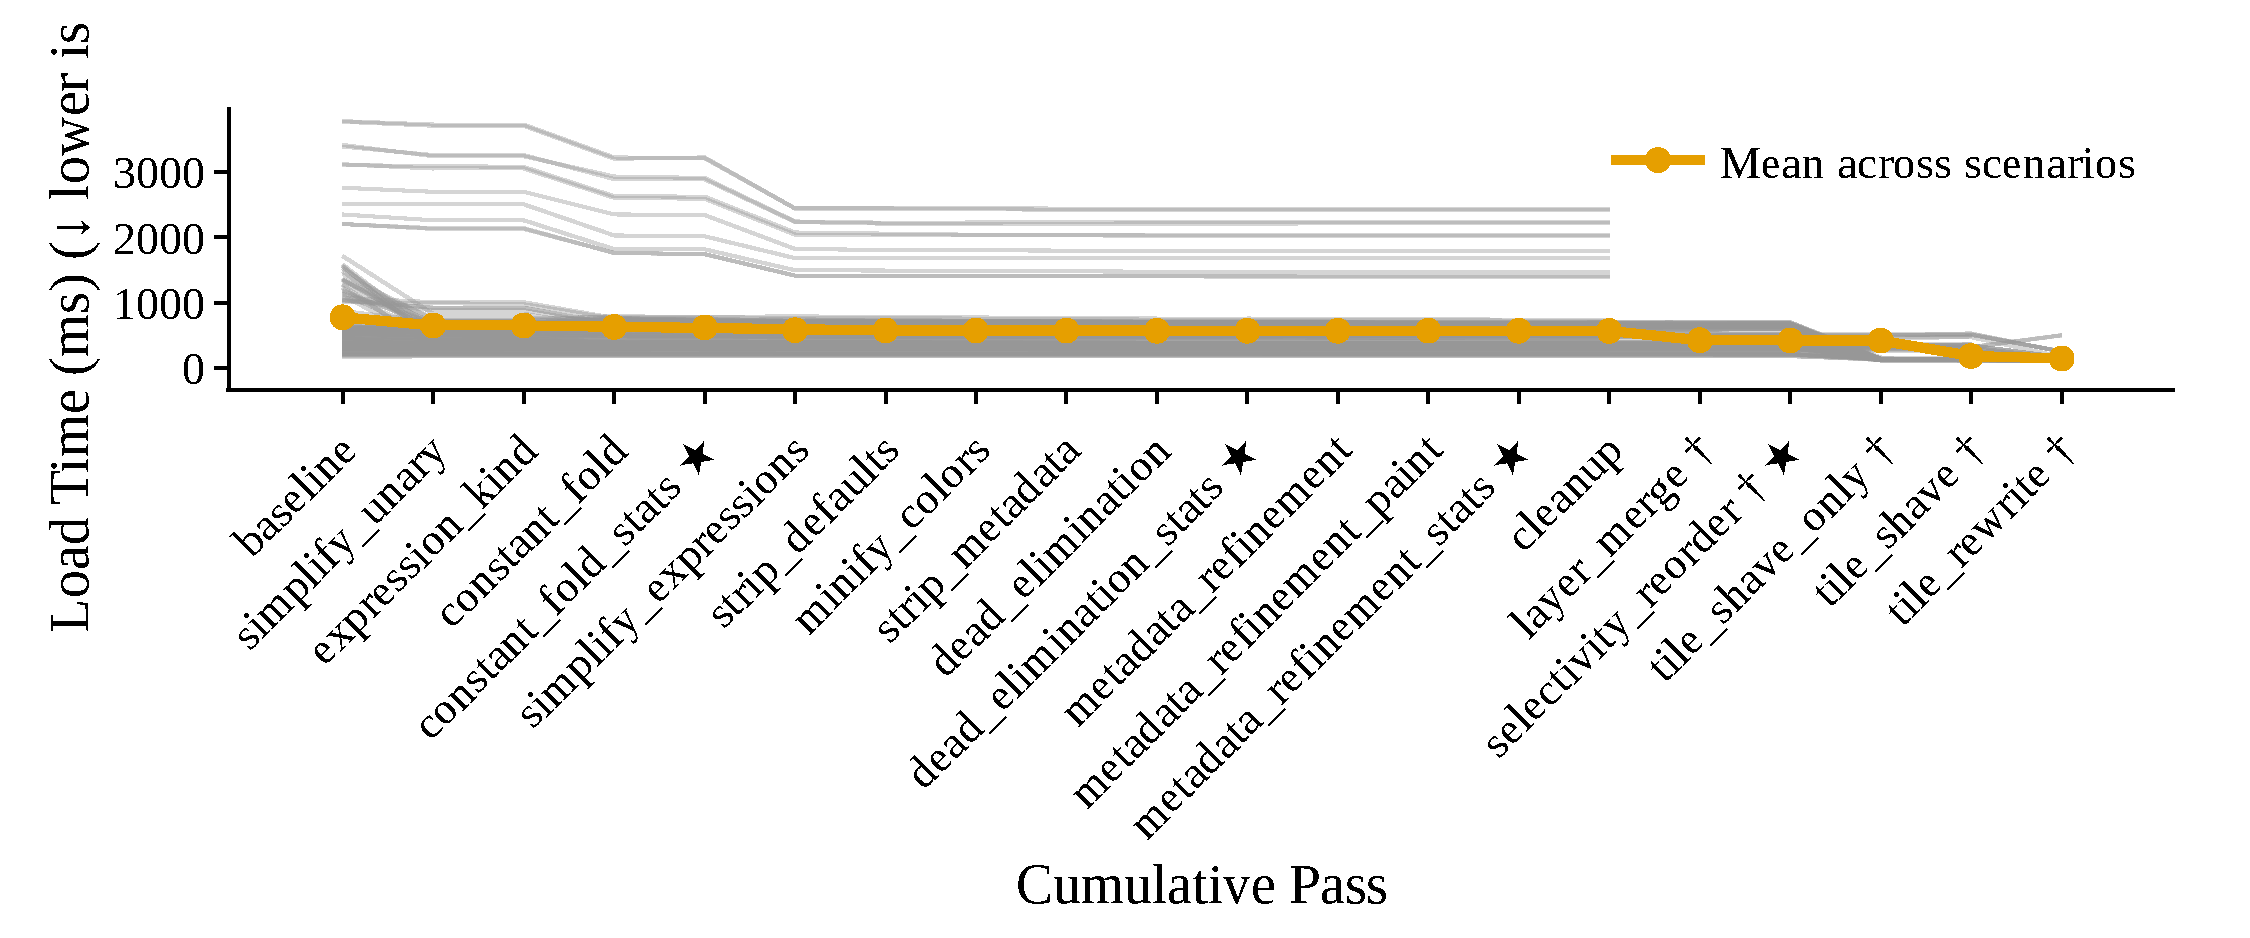
\includegraphics[width=\linewidth]{figures/waterfall_loadMs.pdf}
    \caption{
Cumulative ablation waterfall for load time.
Each bar shows the median change introduced by adding one expression pass on top of all previous passes, aggregated across all 18 scenarios and 15 benchmark styles.
We can see that in the extremes, unary simplifcation has the largest effect.
The aggregate load-time improvement across all expression passes is modest (\qty{-1.8}{\percent}), with expression passes serving primarily as enablers for downstream structural and data-level passes.
For caveats, please see \cref{sub:expr_discussion}}
    \label{fig:waterfall_loadMs}
\end{figure}

\begin{figure}[htbp]
    \centering
    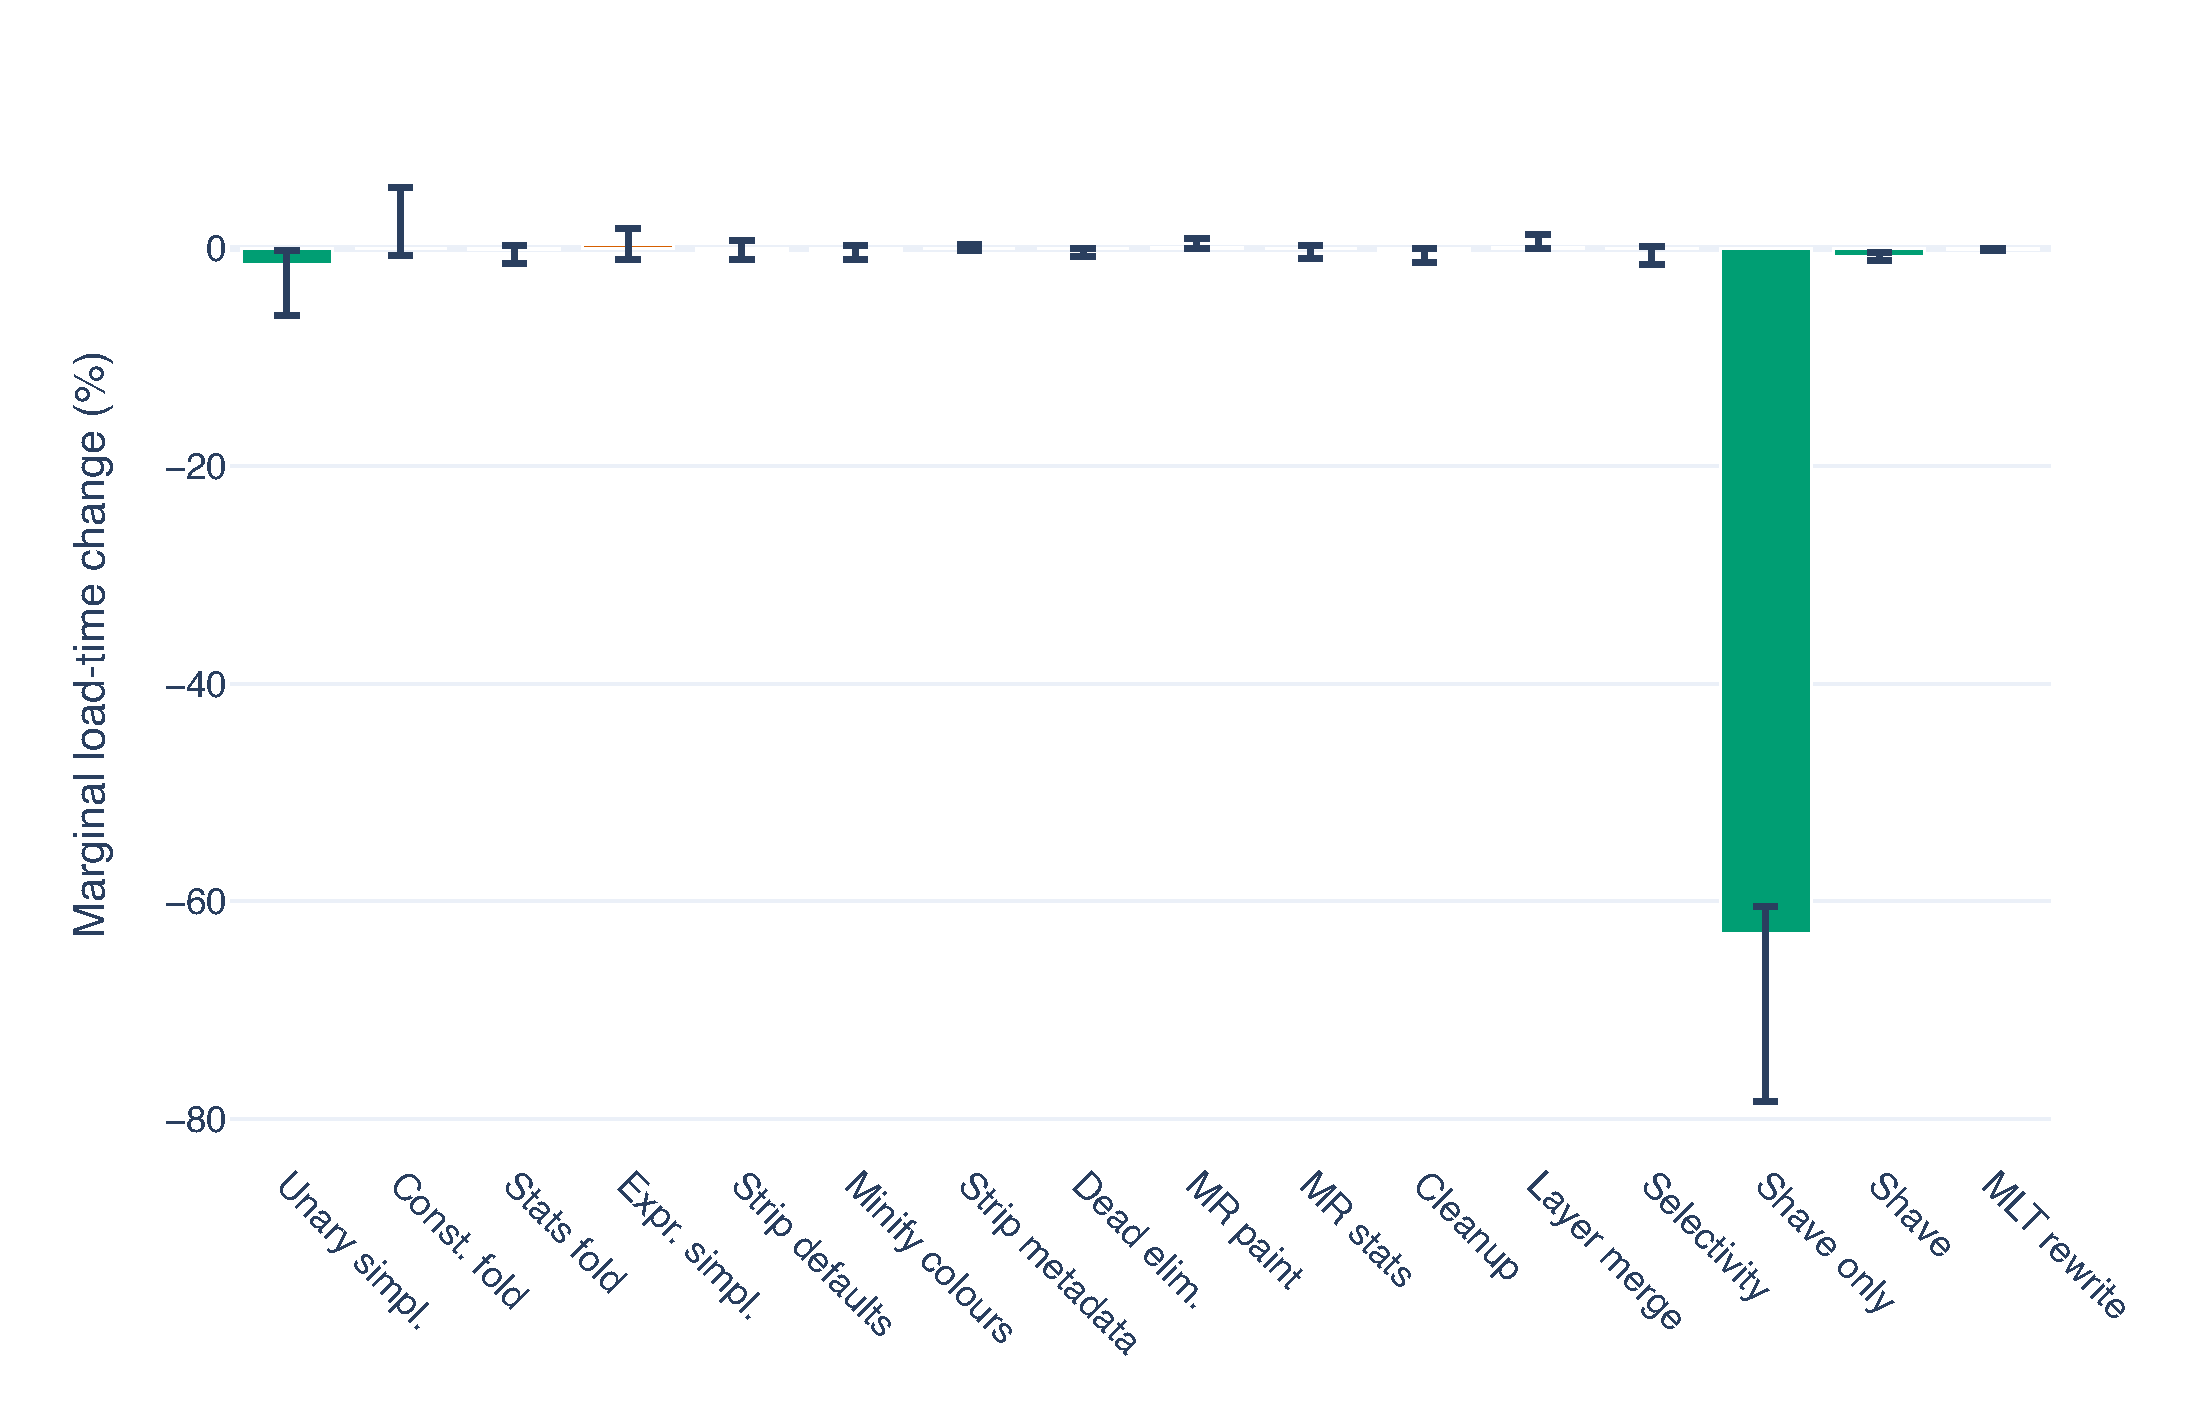
\includegraphics[width=\linewidth]{figures/marginal_loadMs.pdf}
    \caption{
Marginal contribution of each expression pass to load time reduction shows the effect of each of the passes cleanly. }
    \label{fig:marginal_loadMs}
\end{figure}

\begin{figure}[htbp]
    \centering
    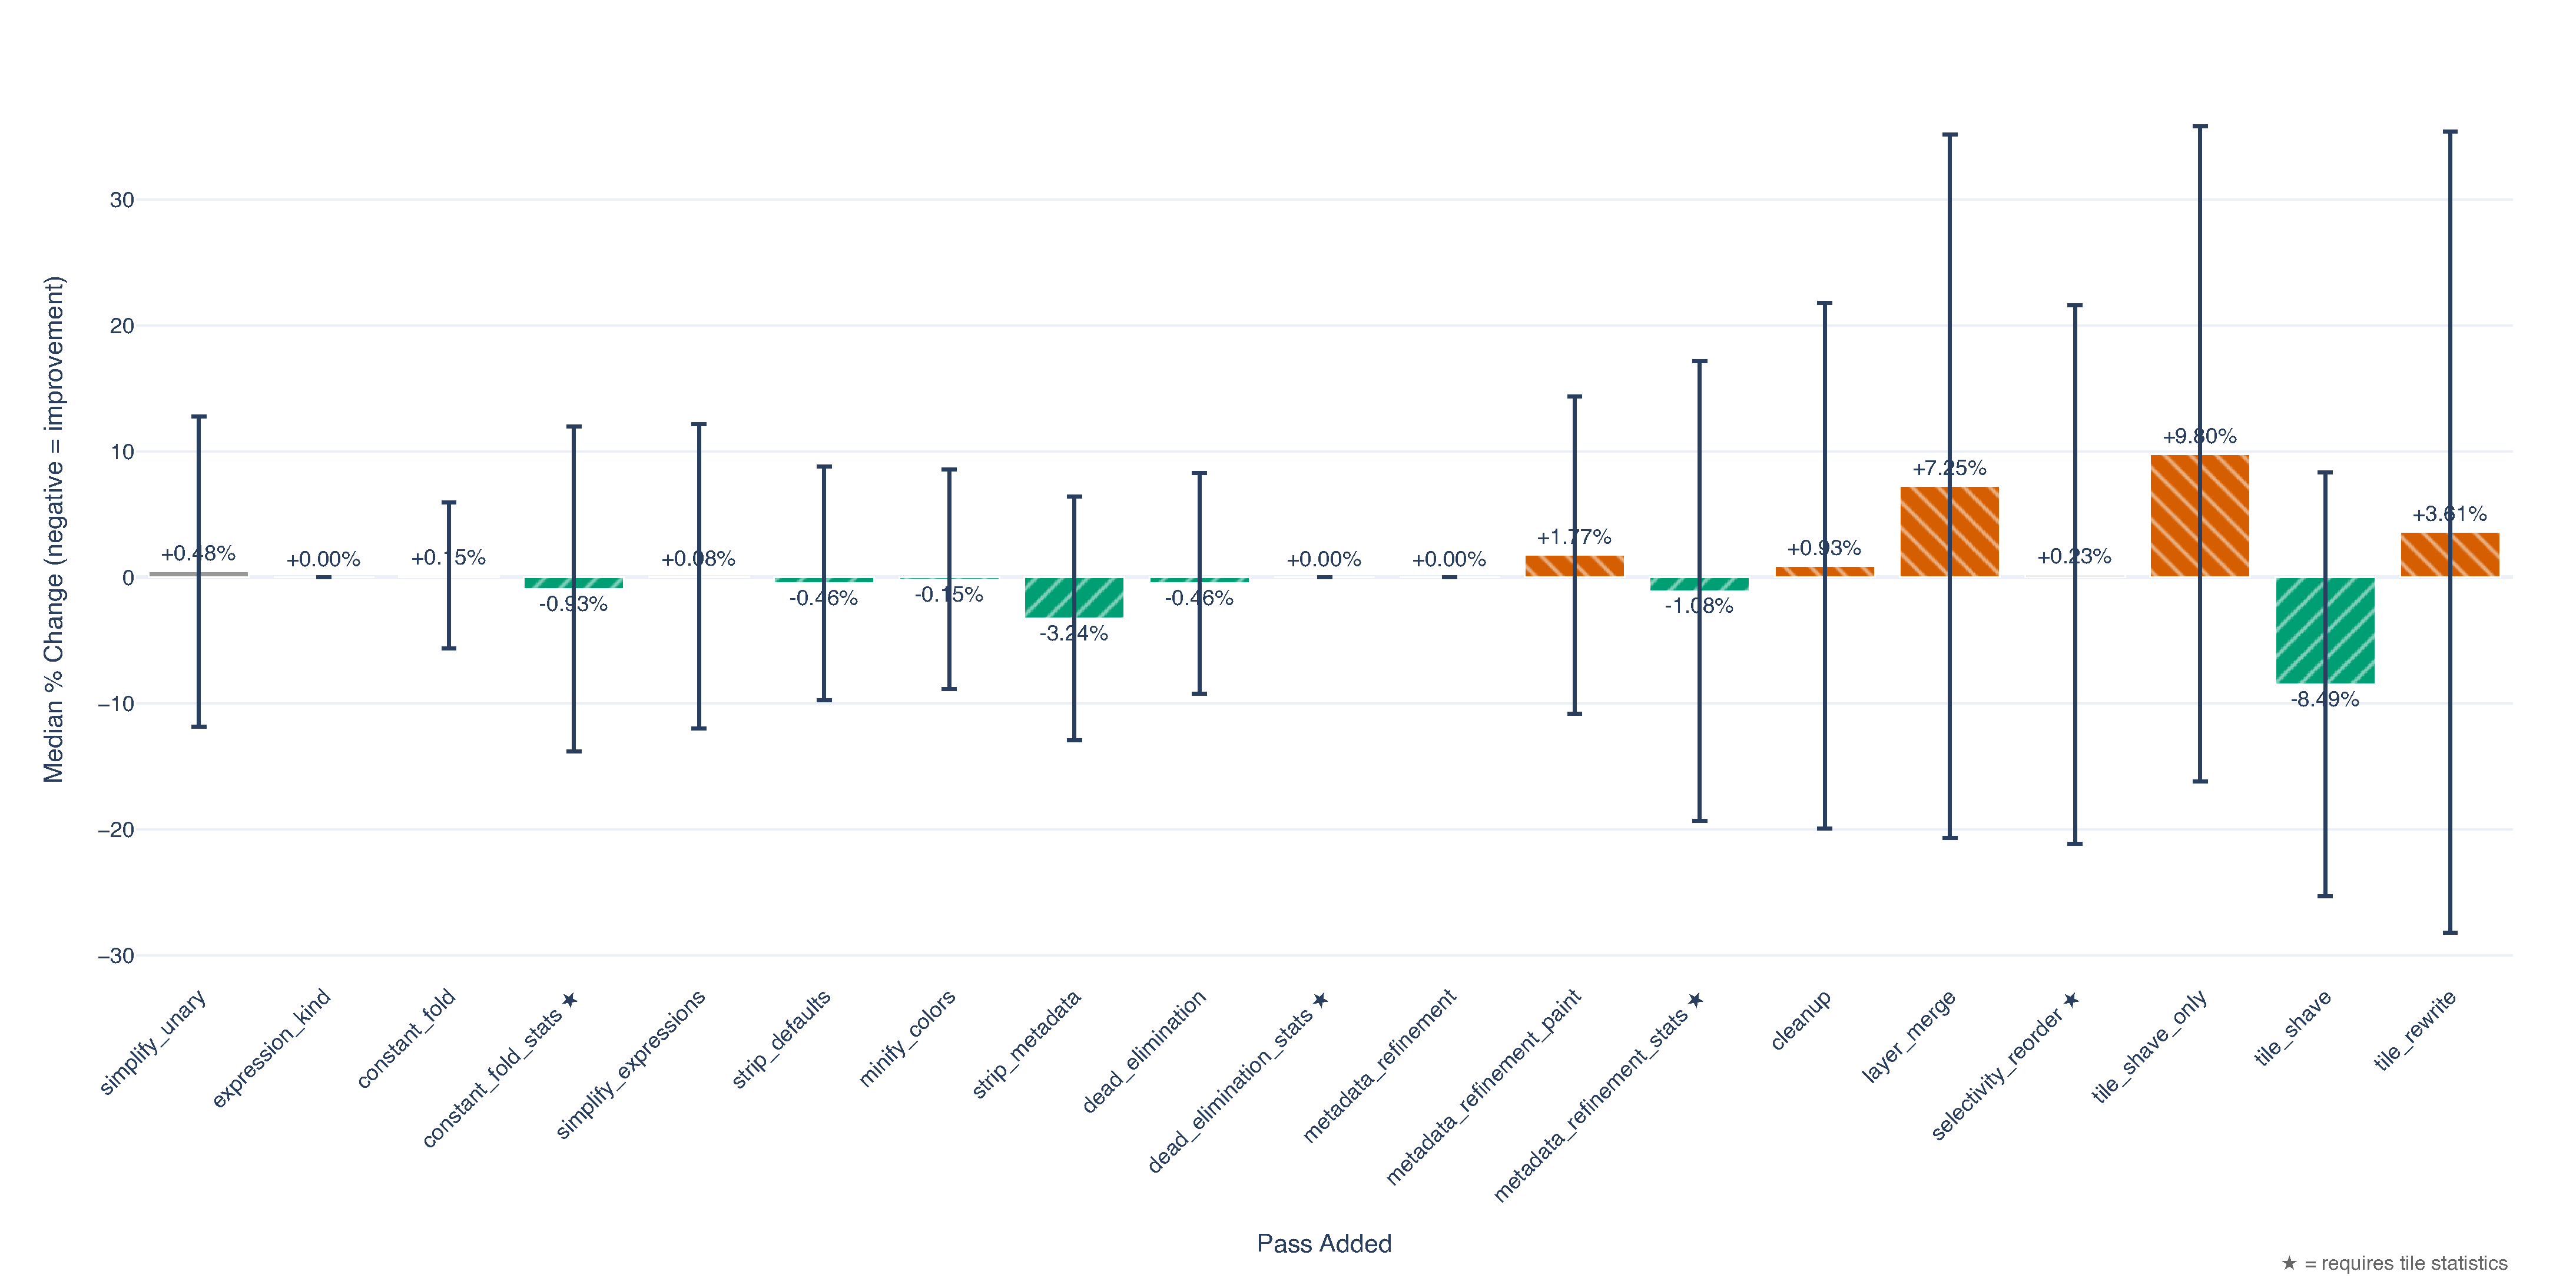
\includegraphics[width=\linewidth]{figures/marginal_styleParseMs.pdf}
    \caption{
Marginal contribution of each expression pass to \texttt{styleParseMs}.
The size-reducing passes (default stripping in particular) shorten the parse step monotonically, even where their end-to-end load-time effect is within noise.
This is the proximate mechanism behind the style-parse leg of the time breakdown in \cref{fig:time_breakdown}.}
    \label{fig:marginal_styleParseMs}
\end{figure}

\subsection{Discussion}\label{sub:expr_discussion}

Expression passes shave only \qty{1.8}{\percent} from median load time, but raw style size drops by up to \qty{20.3}{\percent} on Fiord, with most of the size win concentrated in a single pass (default stripping).
We use the rest of this section to explain why one outlier pass dominates the per-style picture and why the size-reduction story diverges from the rendering-time one.

\paragraph{Dominance of Unary Simplification}
Some styles are implemented in a not optimal way and thus allow a very high unary simplification gain.
The gain of this simplification is non-representative and biases the results to look better than they are overall.
Only two of the style familys gain significant speedups, both of the times through what we think are typos in how the style is written.

We expect this.
Reducing an expression tree to a literal eliminates all per-feature evaluation cost for that expression, whereas algebraic simplifications merely shorten the evaluation path.
For some styles this does not hold and unary simplification is more effective due to expensive string index handling being collapsed into senatically identical, but faster variants.
Fixpoint iteration amplifies the effect.
A single successful simplfication can cascade through nested expressions, collapsing entire subtrees in subsequent iterations.

\paragraph{Size Reduction vs.\ Rendering Improvement}
Passes that primarily reduce serialized style size (default stripping, color minification) show smaller rendering improvements but contribute meaningfully to transfer size under compression.
This primarily benefits time to first render (discussed in \cref{sub:combined_marginal}).
We note the distinction between raw, gzip, and Brotli reductions: some rewrites (e.g., \mlop{\texttt{any}}$\to$\mlop{\texttt{in}}) increase raw token count while decreasing compressed size, because the repetitive structure of \mlop{\texttt{in}} operand lists compresses well.

\paragraph{Empirical Coverage of Selectivity Reordering}
Selectivity reordering (step~16) is a theoretically motivated heuristic whose isolated rendering impact we did not measure in this evaluation.
Because it appears late in the cumulative ablation, its marginal contribution is confounded with the preceding passes.
We acknowledge the independence assumption underlying the selectivity estimates as inaccurate for correlated map predicates (\cref{sec:query_optimizations}), and the empirical benefit may be negligible for styles whose filters are already short.

\paragraph{Downstream Interaction with the Data Pipeline}
Beyond their direct rendering benefit, expression-level simplifications feed into the data-level pipeline evaluated in \cref{sec:exp_mlt}.
Each folded filter predicate and each pruned \mlop{\texttt{match}} arm reduces the set of property names and categorical values that the tile pruning advisory (\cref{sub:tile_shaving}) must track.
Each filter reduced to \mlval{\texttt{false}} enables dead layer elimination in the structural phase, which removes that layer's entire property footprint from the advisory.
Simpler filters are also more amenable to the advisory's static analysis, because canonical forms (e.g., a direct \texttt{[\mlop{"=="},~\ldots]} rather than a double-negated comparison) expose referenced property values more readily.
The magnitude of this interaction is quantified in \cref{sec:exp_mlt}.


\section{Experiment 2: Structural Optimizations}\label{sec:exp_structural}
\begin{keytakeaways}
\item Dead-layer elimination and layer merging produce nearly all the structural-family gains;\newline
      the other passes are negligible on their own.
\item Layer merging can grow raw bytes yet still shrink frame time.
Gzip absorbs the difference.
\item Symbol-heavy styles benefit less because symbol layers are excluded from merging.
\end{keytakeaways}

\noindent Where the previous experiment rewrote local expressions, in this one we evaluate the passes that reason across layers and sources: the structural family of \cref{sub:structural_optimizations}.

\subsection{Pass Interactions}\label{sub:structural_interactions}

Several pairwise dependencies between structural passes shape what we measure in the cumulative ablation in \cref{sub:structural_results}.
Expression passes must run first so that metadata refinement sees zoom predicates in their canonical form.
Dead elimination must precede layer merging because a dead layer between two otherwise-mergeable live layers blocks the merge.
Similarly, metadata refinement must precede cleanup so the residual \mlval{\texttt{true}} filters and zero-opacity layers it produces can be removed.
We give the full ordering rationale in \cref{sub:pipeline}.
The practical consequence here is that the marginal contribution of each later pass in the ablation will reflect work that an earlier pass enabled, not just the pass itself.

\subsection{Evaluation}\label{sub:structural_evaluation}

Structural passes correspond to ablation steps~8-15 within the cumulative ablation of \cref{sub:ablation}.
In addition to the rendering metrics from Experiment~1 (\cref{sub:metrics}), we report complexity metrics for the structural evaluation: layer count, filter count, and total expression node count.
We report the effects on performance generalized in \cref{sub:cross_results} (over the generalization corpus of \cref{sub:generalization_corpus}) and the effect of the expression-level steps this work builds upon in \cref{sec:exp_expressions}.

\subsection{Results}\label{sub:structural_results}

\cref{fig:complexity_layer_count} tracks layer count across the structural ablation steps, showing which passes concretely remove layers rather than merely rewriting them.
\cref{fig:complexity_total_expression_nodes,fig:complexity_filter_count} extend the complexity view to the two remaining metrics introduced in \cref{sub:structural_evaluation}: total expression-tree node count and filter count.
\cref{fig:style_size_ablation} complements these with the raw, gzip, and Brotli style sizes, confirming that the structural reductions also translate into smaller transfer size rather than just reshuffling the serialized form.


\begin{figure}[htbp]
	\centering
	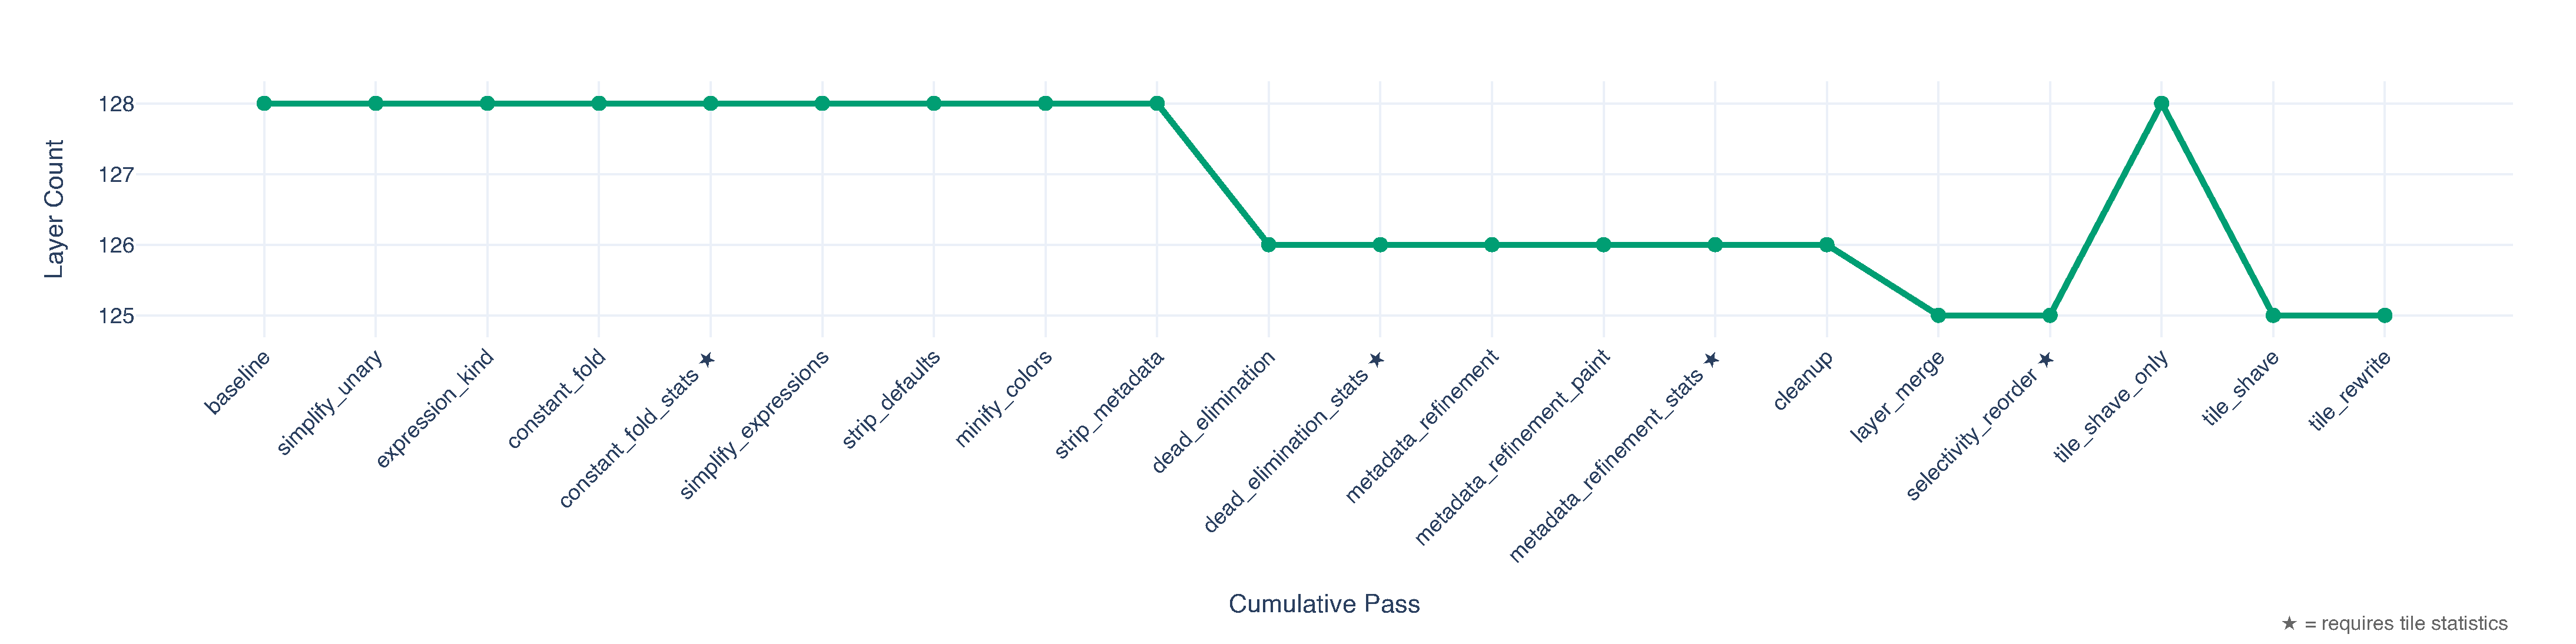
\includegraphics[width=\linewidth]{figures/complexity_layer_count.pdf}
	\caption{
Layer Count across Cumulative Ablation Steps on the Liberty Style: only layer merging reduces the layer count.
Dead elimination rarely removes whole layers, because styles are designed to expose parts of the map rather than leave entire layers unreferenced.}
	\label{fig:complexity_layer_count}
\end{figure}

\begin{figure}[htbp]
	\centering
	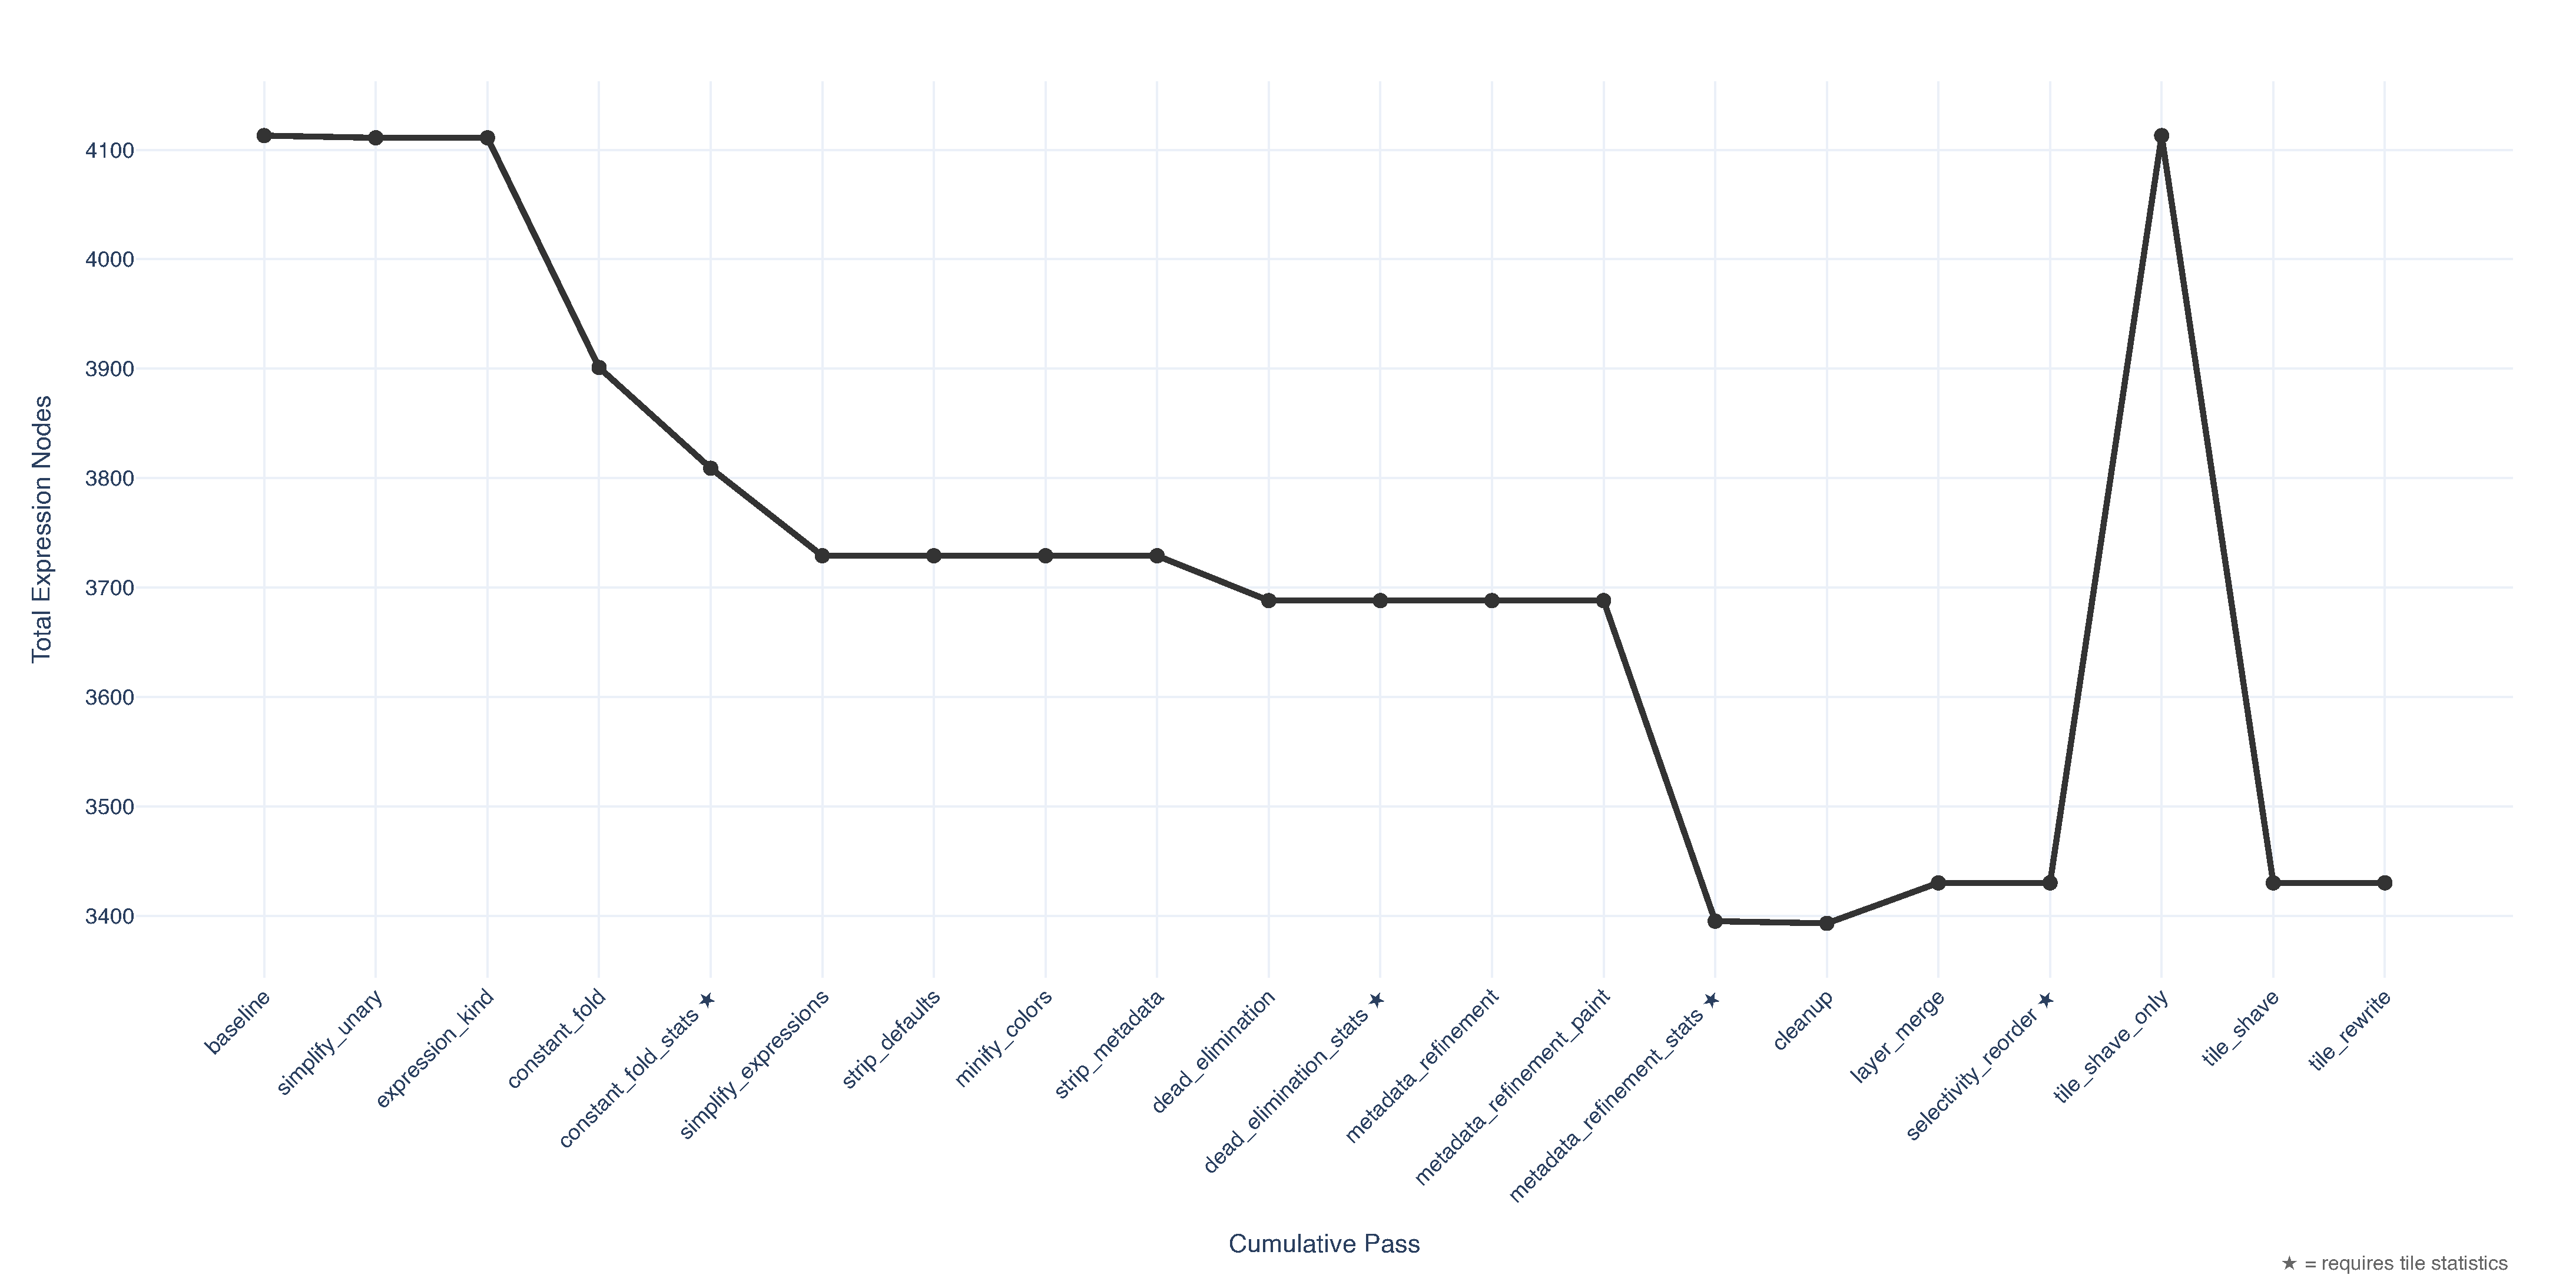
\includegraphics[width=\linewidth]{figures/complexity_total_expression_nodes.pdf}
	\caption{
Total expression-tree node count across cumulative ablation steps.
Expression passes (steps~1-7) produce the largest reductions, with Fiord dropping by \qty{36.8}{\percent} (\num{1610}$\to$\num{1018}) and Liberty by \qty{10.5}{\percent} (\num{3537}$\to$\num{3167}).
Structural passes contribute additional, smaller reductions by removing or merging layers that own subtrees.}
	\label{fig:complexity_total_expression_nodes}
\end{figure}

\begin{figure}[htbp]
	\centering
	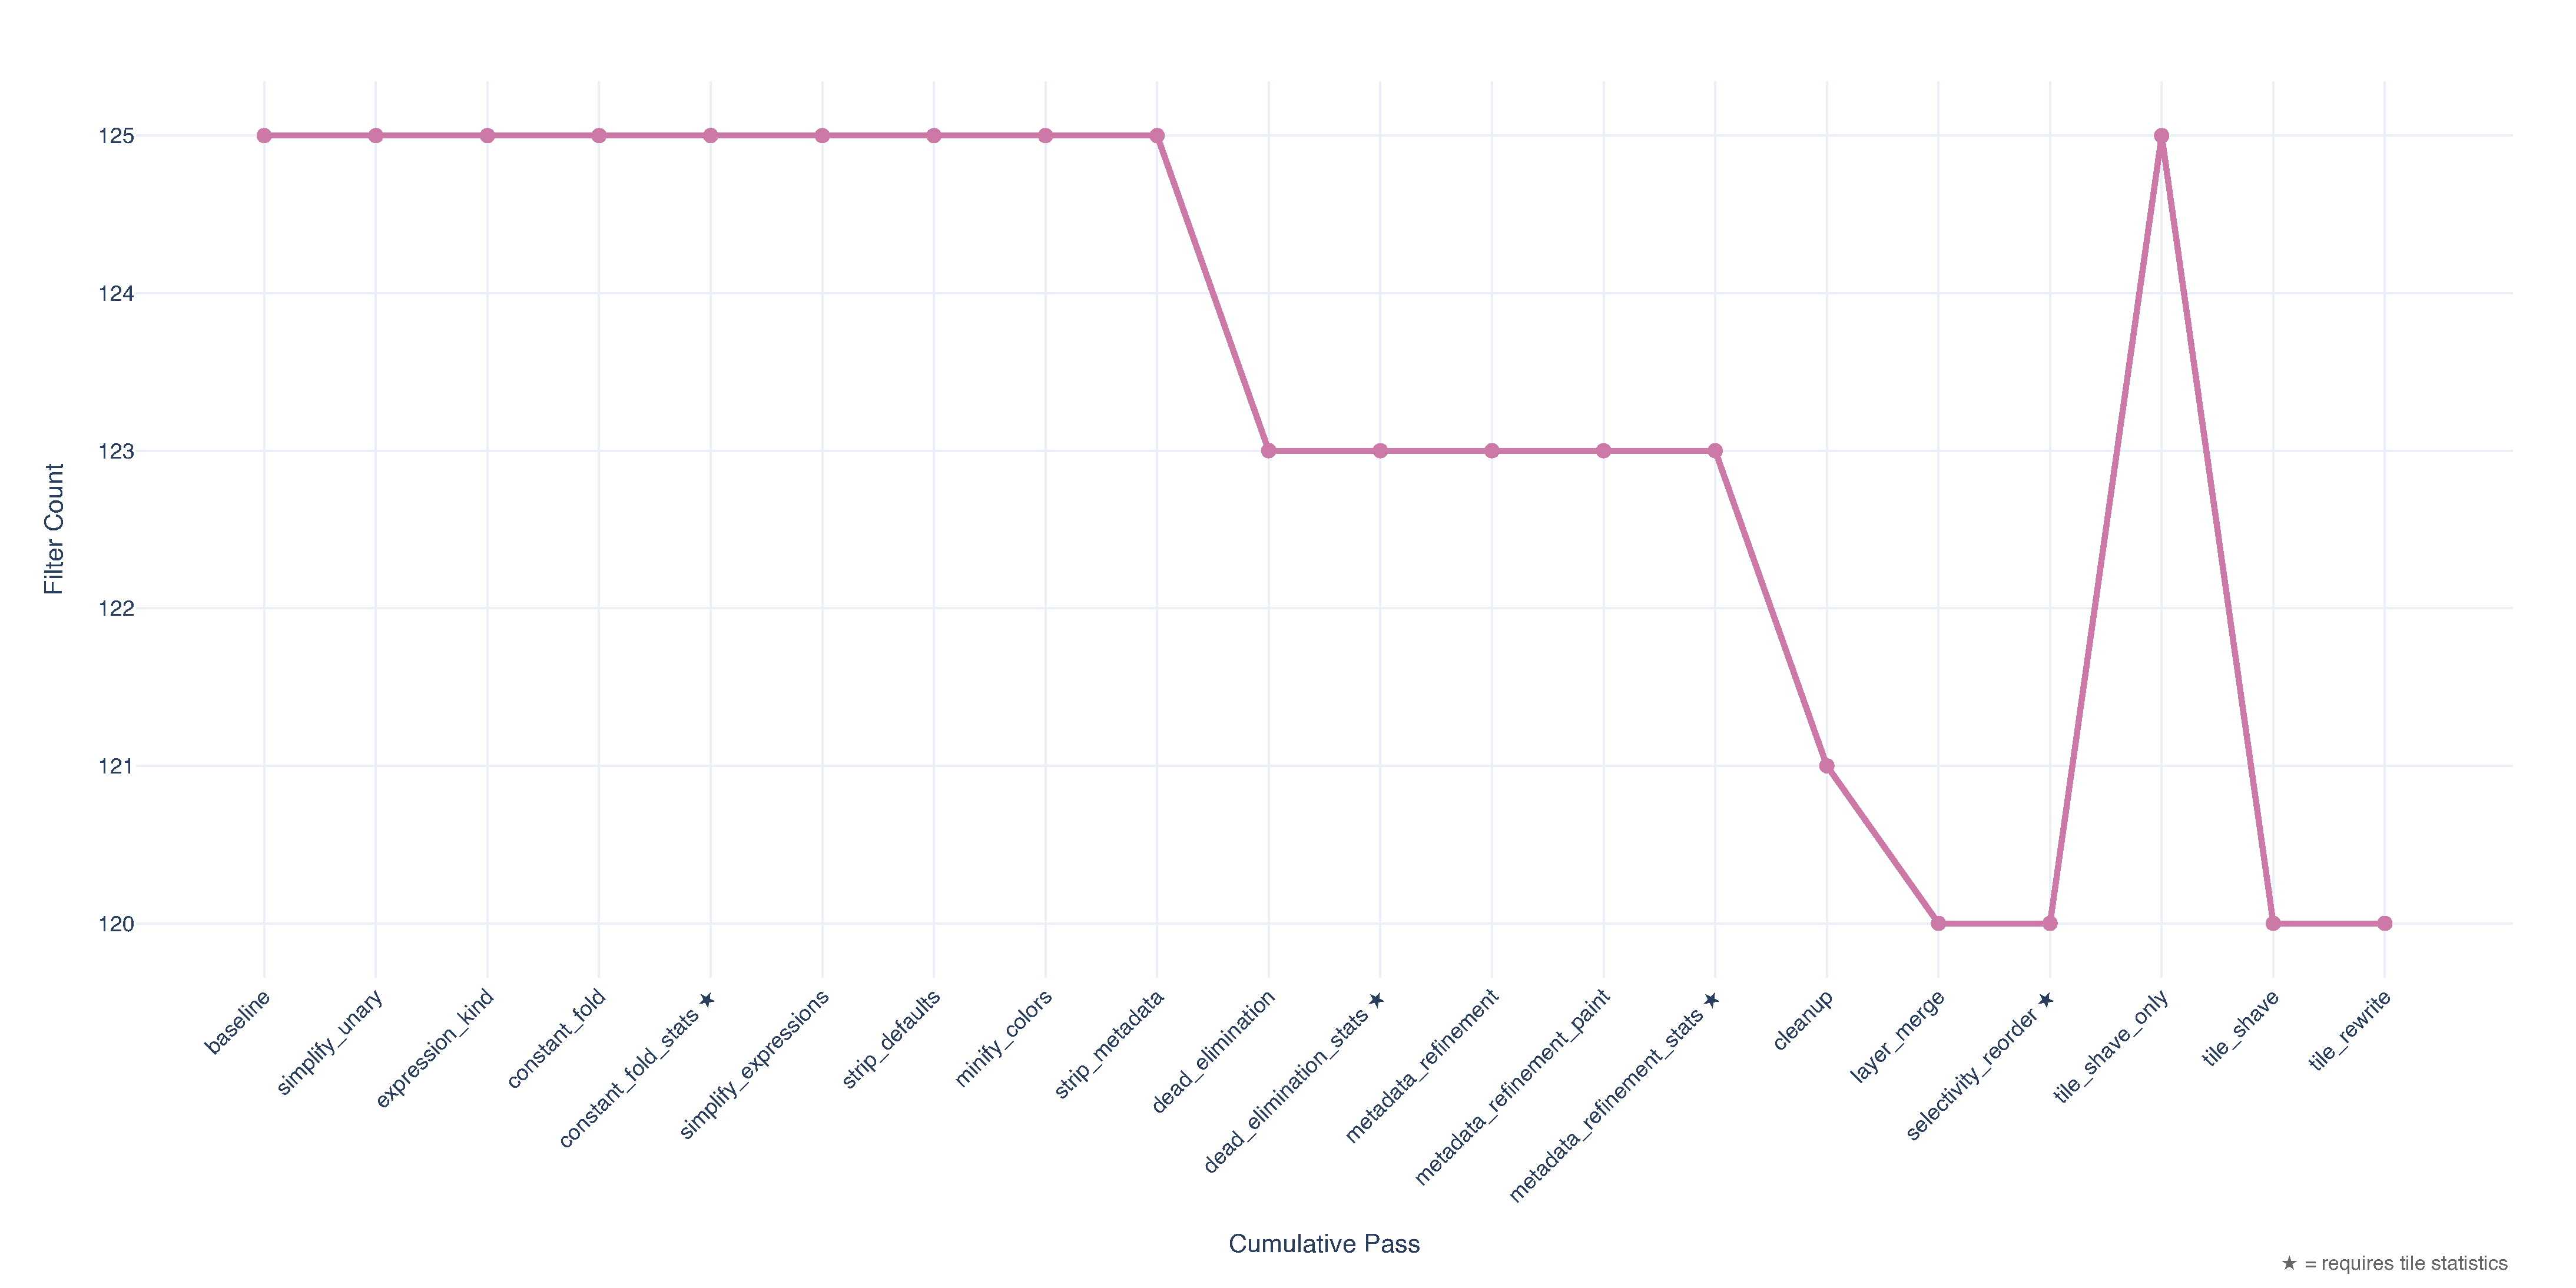
\includegraphics[width=\linewidth]{figures/complexity_filter_count.pdf}
	\caption{
Filter count across cumulative ablation steps.
Metadata refinement (consuming zoom predicates) and dead elimination drive most of the filter-count reduction.
Cleanup removes the residual \mlval{\texttt{true}} filters that refinement leaves behind.}
	\label{fig:complexity_filter_count}
\end{figure}

\begin{figure}[htbp]
	\centering
	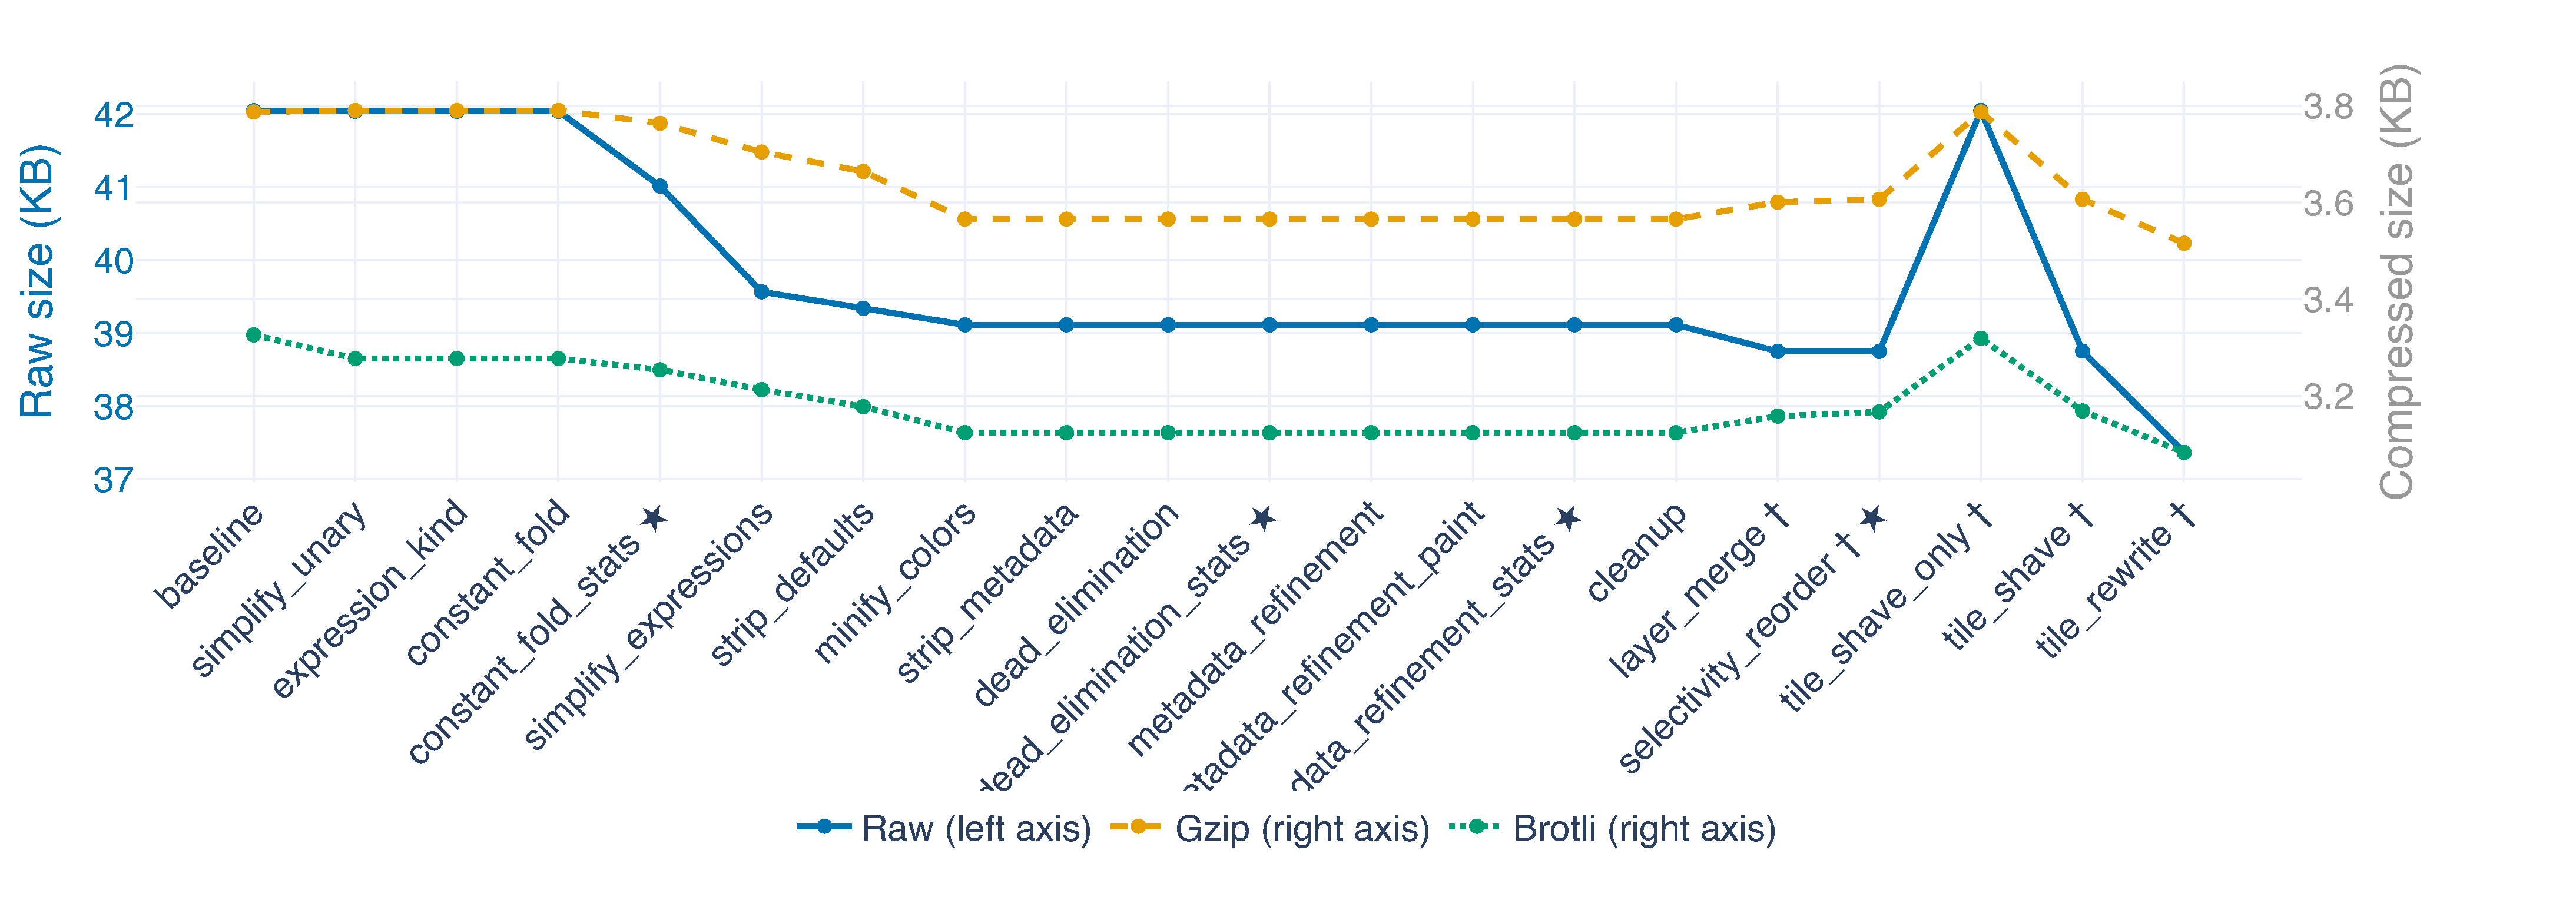
\includegraphics[width=\linewidth]{figures/style_size_ablation.pdf}
	\caption{
Style size (raw, gzip, Brotli) across ablation steps: the effect on this metric is incremental rather than transformative.}
	\label{fig:style_size_ablation}
\end{figure}

The magnitude of structural improvement is style-dependent.
Fiord's 48-layer style sheds two layers (\qty{-4.2}{\percent}), one from dead elimination (step~9) and one from cleanup (step~14) after metadata refinement reduces a filter on an invisible layer to \mlval{\texttt{true}}.
The drop translates to \qty{-14.1}{\percent} gzip transfer and \qty{-36.8}{\percent} fewer expression-tree nodes (\num{1610}$\to$\num{1018}).
Liberty's 111 layers shed four (\qty{-3.6}{\percent}), concentrated in the layer-merge step (step~15), which combines four pairs of adjacent layers with compatible filters for \qty{-4.9}{\percent} gzip and \qty{-10.5}{\percent} nodes (\num{3537}$\to$\num{3167}).
Layer merging itself adds \qty{36}{\byte} of gzip because the merged filter expressions are wordier.

\subsection{Discussion}\label{sub:structural_discussion}

Two of the six structural passes (dead-layer elimination and layer merging) produce nearly all of the gain, cutting Fiord's gzip transfer by \qty{14.1}{\percent} and Liberty's by \qty{4.9}{\percent}.
The following paragraphs unpack why those two dominate and how the remaining passes contribute indirectly or feed into the data-level pipeline downstream.

\paragraph{Dominance of Dead Elimination and Layer Merging}
Among the structural passes, dead elimination and layer merging produce the largest improvements in both rendering performance and style complexity.
Dead elimination directly reduces the number of layers the renderer must process per frame.
Layer merging reduces draw calls by combining multiple rendering passes into one.
The interaction between the two is synergistic: styles with many narrowly-filtered layers (e.g., road styles that define separate layers for each road class) benefit most, as dead elimination first removes layers for road classes absent from the data, and layer merging then combines the remaining layers into a single multi-class layer.

\paragraph{Size vs.\ Runtime Trade-Off in Layer Merging}
Layer merging does not always reduce the raw serialized byte count.
A merged layer replaces $k$ small filter expressions with a single \mlop{\texttt{match}}-keyed filter and $k$-armed \mlop{\texttt{match}} expressions for every differing paint property, which for small $k$ can produce a slightly larger textual representation than the sum of the originals.
The per-style ablation tables in \cref{sec:app_per_style} show one such case (Bright: \num{44.4}$\to$\qty{44.6}{\kilo\byte} after layer merging), where the raw count creeps up while the layer count drops by one (119$\to$118).
This was uncomfortable when we first saw it in the runs, since the intuition is that merging should shrink the style, but raw byte count turns out to be a proxy for parse time and transfer cost rather than for rendering cost, which is driven by layer count and per-frame draw calls.
The merged layer is still cheaper to render even when its serialized form is bigger, and the gzip and Brotli columns of the same table show the compressed size essentially unchanged, so the raw increase disappears under realistic wire compression anyway.

\paragraph{Indirect Effects of Metadata Refinement}
Metadata refinement does not directly reduce the number of layers or the complexity of expressions.
Instead, it enables the renderer to skip layers at zoom levels where they are invisible.
The rendering improvement is therefore zoom-dependent.
At overview zoom levels (where many layers are filtered out by tightened \texttt{minzoom}) the improvement is large, and at street-level zoom (where most layers are active) the improvement is smaller.
Paint-based refinement captures a class of optimizations that are invisible to filter analysis.
A layer whose opacity interpolates from~0 at zoom~12 is indistinguishable from a fully visible layer when examining only the filter.

\paragraph{Amplification of Style-Only Passes by Stats-Driven Passes}
The marginal contribution of stats-driven dead elimination (step~10) over non-stats dead elimination (step~9) quantifies the value of tile statistics for style optimizations.
Styles that use broad \texttt{source-layer} references benefit most, as statistics reveal which geometry types and property values actually exist.
For styles that already have precise filters (e.g., hand-tuned Americana), the marginal gain is smaller.

\paragraph{Symbol Layer Exclusion}
We exclude symbol layers from merging because MapLibre's collision detection operates per-layer (we give the soundness argument in \cref{sub:structural_optimizations}).
The headline merging numbers above are therefore reductions in the non-symbol pool only.
Because styles are usually dominated by labels, most see proportionally smaller layer-count gains.

\paragraph{Downstream Interaction with Tile Shaving}
Dead layer elimination has a second-order effect beyond reducing per-frame draw calls:
each eliminated layer removes its property references from the tile pruning advisory computed in the data-level pipeline (\cref{sub:tile_shaving}).
If a removed layer was the sole consumer of a property column, that column is stripped from every tile at encoding time.
Similarly, metadata refinement's tightened zoom bounds cause the advisory to mark additional zoom levels as unused for a given source-layer, potentially eliminating entire tiles.
We characterize this interaction fully in \cref{sub:mlt_discussion} and quantify it in \cref{sub:mlt_results}.
The aggregate data shows that the composition is additive rather than synergistic, but the advisory-narrowing effect is a necessary precondition for style-dependent tile shaving.


\section{Experiment 3: Data-Level Optimizations}\label{sec:exp_mlt}
\begin{keytakeaways}
\item Tile shaving dominates with a \qty{-71.5}{\percent} median load reduction, and style passes contribute additively, not synergistically.
\item The \ac{MLT} format alone is not the win.
The reference \ac{MLT} encoder drifts above $1.0\times$ \ac{MVT} under gzip/Brotli.\newline
    The gain comes from the strategy competition and shared-dictionary selection in our encoder.
\end{keytakeaways}

\noindent In \cref{sec:exp_structural,sec:exp_expressions} we optimized the \emph{program} the renderer executes.
In this experiment we ask whether we can optimize the \emph{data} it consumes using the same style information, and to what extent the two levels interact.
This is the joint-optimization question at the heart of Research Goal~R1 and formalised in \cref{sec:problem_statement}.
The data-level pipeline we apply here (\cref{sub:data_optimizations}) takes the optimized style and uses it to drive the tile pruning advisory and the encoding strategy competition.

\textit{We carried out this experiment in collaboration with Rivian Automotive, Inc to optimize performance, correctness, and software architecture of the encoder-decoder pair.
We implemented the encoder and its strategy-selection routine ourselves.
Rivian contributed the runtime performance engineering, which brings transcoding of the Germany OpenMapTiles tileset down from roughly five hours under the prior Tremmel \& Zink reference encoder to about one minute.
We credit that speedup to Rivian rather than ourselves, and therefore do not analyse encoder performance further in this chapter.}

\subsection{Problem Statement}\label{sub:mlt_problem}

Beyond the thesis-wide formal optimization problem of \cref{sec:problem_statement}, two open problems specific to the data-level pipeline frame this experiment:

\begin{enumerate}
    \item \textbf{Tiles carry data the style never uses, and how much depends on the style.}
    A general-purpose tile schema (e.g., OpenMapTiles) exposes hundreds of properties and multiple geometry types.
Any specific style references only a fraction.
    The unused remainder is style-dependent, so the savings achievable by tile shaving (\cref{sub:tile_shaving}) co-vary with the upstream style optimizations:
    more dead layers and simpler filters expose more removable columns and feature values.

    \item \textbf{Encoders ignore the data characteristics that shaving produces.}
    Existing \ac{MLT} encoders commit to a fixed encoding plan per column.
    After shaving, the surviving data has fewer distinct values, longer runs, and smaller string vocabularies, which a data-adaptive encoder (\cref{sub:encoding_strategies}) can exploit but a fixed-plan encoder cannot.
\end{enumerate}

\subsection{Evaluation Design}\label{sub:mlt_evaluation}

In this experiment we isolate the interaction between style-level and data-level optimizations and identify which level contributes the dominant share of the end-to-end savings.
We use a cumulative design with five configurations, each adding one optimization layer:

\begin{enumerate}
    \item \textbf{\ac{MVT} baseline}: unoptimized protobuf-encoded tiles served with the original style.
    \item \textbf{Style-only}: the optimized style from Experiments~1-2, served with unmodified \ac{MVT} tiles.
    \item \textbf{Shaving-only}: the original style with tile shaving applied (advisory-driven pruning of unused columns, geometry types, and property values), but without style optimizations.
    \item \textbf{Style + shaving}: The optimized style driving tile shaving.
    Dead layer elimination and metadata refinement may narrow the advisory relative to the unoptimized style.
    \item \textbf{Style + shaving + \ac{MLT} encoding}: encoding stage that delivers the shaved data to the wire via automatic encoding strategy selection (sort competition, per-stream profiling, string compression).
\end{enumerate}

\noindent Configurations~2-4 isolate the interaction effect.
If the combined reduction of style+shaving exceeds the sum of style-only and shaving-only, the two optimization categories are synergistic.
If approximately equal, they compose additively.
If less, they are partially redundant.
Configuration~5 adds the encoding layer: after shaving has determined what data survives, the multi-strategy competition adapts to the statistical properties of the surviving data.
Those properties differ from the unshaved original because shaving has removed columns and features, altering value distributions and run-length characteristics.

For each configuration, we collect two classes of metrics: \emph{tile transfer metrics} (encoded tile size in raw, gzip, Brotli per zoom level, total tileset volume, and encoding time per tile) and \emph{rendering metrics} shared with Experiments~1-2 (load time, frames per second, frame time percentiles p50/p95/p99, and time to first tile), enabling direct comparison of data-level contributions against expression-level and structural contributions in the combined analysis (\cref{sec:exp_combined}).

\subsection{Results: Style-Driven Cascade}\label{sub:mlt_results}

In this section we quantify the interaction between style-level and data-level optimizations previewed in \cref{sub:structural_discussion}: style-level optimizations narrow the pruning advisory, and in the following paragraphs we measure the extent of this effect before turning to the encoding evaluation.

\paragraph{Interaction between Style and Data Optimizations}
Comparing gzip-size reductions for style-only, shaving-only, and the combination: Fiord's combined reduction (\qty{14.7}{\percent}) sits \qty{0.2}{\percent} above its style-only figure (\qty{14.5}{\percent}), and Liberty's combined (\qty{4.8}{\percent}) matches its style-only (\qty{4.8}{\percent}).
Both styles compose additively.
Shaving alone is negligible for these two because Liberty references most tile properties and Fiord's gains already come from layer-level cleanup.
This was the central empirical question of the thesis and the one we expected to answer in the affirmative going in.
The data returned additivity, not synergy.
Per-scenario load-time synergy (combined exceeding the sum) appears in 17 of 36 style-scenario pairs but is too sparse to lift the aggregate.

\paragraph{Rendering Metrics across Configurations}
\cref{fig:rendering_metrics_mlt} reveals that the dominant rendering improvement comes from tile shaving rather than style optimizations.
Headline numbers in this paragraph are pooled medians across raw Fiord and Liberty runs.
Per-style equivalents for the ten deep-corpus styles appear in \cref{tab:per_style_summary} and the chapter summary.
Shaving-only drops the pooled median load time from \qty{424}{\milli\second} (baseline) to \qty{121}{\milli\second} (\qty{-71.5}{\percent}).
Style-only contributes a modest \qty{-4.1}{\percent}, and style+shaving reaches \qty{-73.3}{\percent}.
\ac{MLT} re-encoding adds a \qty{+5}{\percent} load-time regression versus the plain-shaving config (\qty{119}{\milli\second} vs.\ \qty{113}{\milli\second}) but achieves \qty{-11.0}{\percent} gzip volume across both styles.
\ac{FPS} mirrors the load-time pattern.
Shaving-only lifts the pooled median from 807 to \num{2289} (\qty{+184}{\percent}), style+shaving reaches \num{2331} (\qty{+189}{\percent}), and the \ac{MLT} variant sits at \num{2232} (\qty{+176}{\percent}, with per-style gains of \qty{+148.1}{\percent} for Fiord and \qty{+149.9}{\percent} for Liberty that sit inside the \qtyrange{100}{200}{\percent} per-style range reported at the chapter end), consistent with the additional decoding cost offsetting the smaller transfer size.
At these frame rates ($>{1000}$~\ac{FPS}) the renderer is largely \ac{GPU}-idle.
We read the metric as available performance headroom on constrained devices rather than a directly observable cost saving on the benchmark host.
The native Rust micro-benchmarks show \numrange{4.6}{8.3}$\times$ higher decode throughput for \ac{MLT} over \ac{MVT}+gzip (\cref{tab:decode_throughput}), but this advantage does not fully transfer to the browser, where the \ac{MLT} decoder we build would need to run as a \ac{WASM} module.
We attribute the dominant bottleneck to the \ac{WASM}-to-JavaScript boundary, since each decoded column must be transferred from \ac{WASM} linear memory into JavaScript-visible typed arrays, incurring per-column copying and \ac{GC} pressure that does not exist in a pure-native pipeline.
Secondary overheads include the restriction to 128-bit \ac{WASM} \ac{SIMD} (whereas native \ac{FastPFOR} exploits AVX2/512) and baseline JIT compilation latency.
Jangda et~al.~\cite{jangdaNotFastAnalyzing2019} measured a 45-55\% slowdown for \ac{WASM} relative to native on SPEC \ac{CPU} benchmarks.
Although the computational gap has narrowed since 2019, the data-transfer boundary cost remains largely unchanged because the \ac{WASM}-JS interface still lacks zero-copy sharing of structured columnar buffers.
As a result, the columnar decoder's advantage materialises primarily on larger, feature-dense tiles where the per-column setup and transfer cost is amortised.
On smaller tiles the per-column dispatch overhead narrows the gap to approximate parity with \ac{MVT}'s single-path protobuf parser.
We are currently working to shift more decoding and data consumption into \ac{WASM} to reduce boundary-crossing overhead.
Bootstrap \qty{95}{\percent} confidence intervals confirm that the full-pipeline load-time improvements are tight: Fiord's final load time is \qty{120.5}{\milli\second} (CI: [\num{119.3}, \num{121.5}]), Liberty's is \qty{133.7}{\milli\second} (CI: [\num{132.9}, \num{134.2}]), both with $p < 10^{-45}$ (Wilcoxon, $n = 270$ for Fiord across 18 scenarios and $n = 254$ for Liberty across 17 scenarios at the full-pipeline pool) against their respective baselines.

\begin{figure}[H]
    \centering
    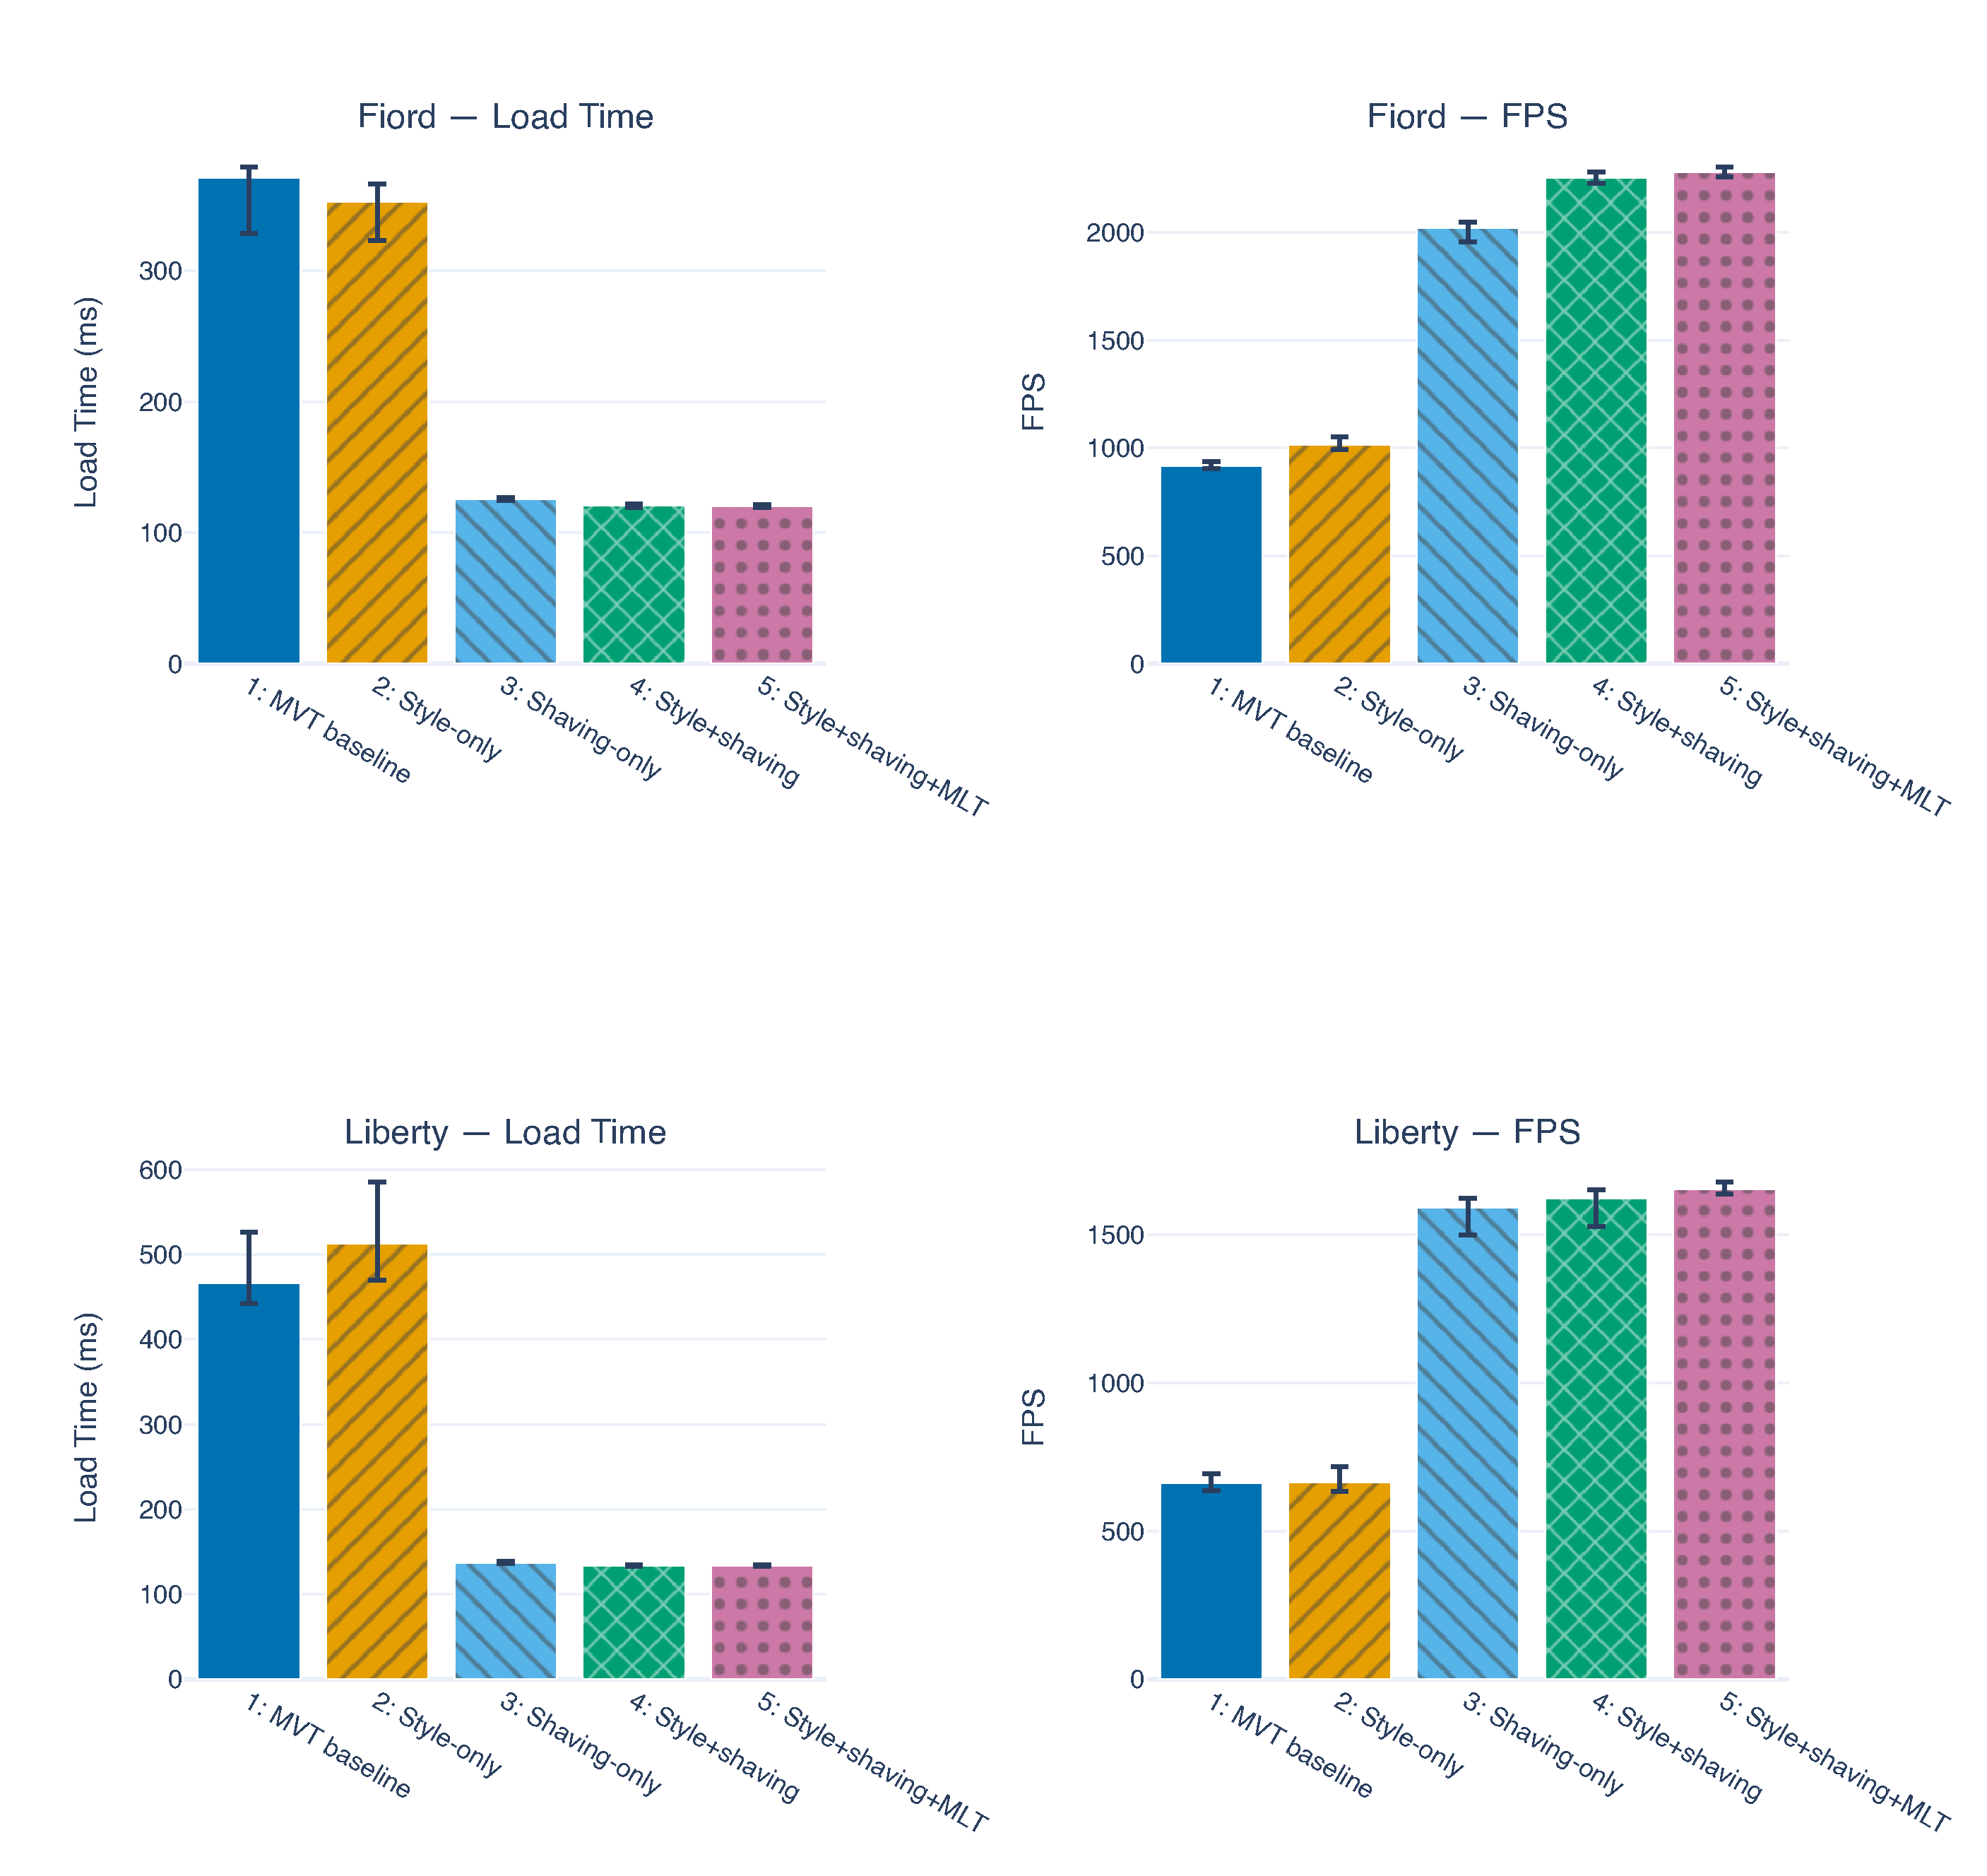
\includegraphics[width=0.9\linewidth]{figures/rendering_metrics_mlt.pdf}
    \caption{
Rendering metrics (load time, \ac{FPS}) across configurations~1-5, enabling direct comparison with Experiments~1-2 in the combined analysis.
The figure shows the significant drop in both load time and increase in \ac{FPS} for tile shaving, as well as the fact that style-only optimization is ineffective.
We also confirm the \ac{MLT} implementation to sligtly decrease performance because the current implementation still internally converts to \ac{MVT}}
    \label{fig:rendering_metrics_mlt}
\end{figure}


\subsection{Results: Encoding the Shaved Data}\label{sub:mlt_encoding_results}

Once shaving has fixed what data survives, the encoding stage determines whether those savings reach the wire.
\cref{fig:shaving_effectiveness_per_zoom} plots total tile size per zoom level for both \ac{MVT} and our \ac{MLT} encoder, with and without shaving via the Liberty advisory.
The gap between each format and its shaved counterpart quantifies the data removed by the pruning advisory.
The gap between the shaved \ac{MVT} and the shaved output of our encoder quantifies the additional contribution of columnar encoding on the already-pruned data.
Both formats benefit from shaving across all compression schemes, confirming that the advisory operates on the data itself rather than relying on format-specific redundancy.
\cref{fig:encoder_comparison} reframes the same evidence as a ratio against the \ac{MVT} baseline, adding the reference \ac{MLT} encoder of Tremmel \& Zink~\cite{tremmelMapLibreTileNext2025b} for comparison: our encoder's curves remain at roughly $0.6$-$0.8\times$ \ac{MVT} throughout the zoom range, whereas the reference-encoder curves drift above $1.0\times$ at several zoom levels under brotli/zstd, underscoring that the gains attributed to the \ac{MLT} format in this thesis come almost entirely from the encoder-side strategy competition and not from the columnar format alone.

\begin{figure}[htbp]
    \centering
    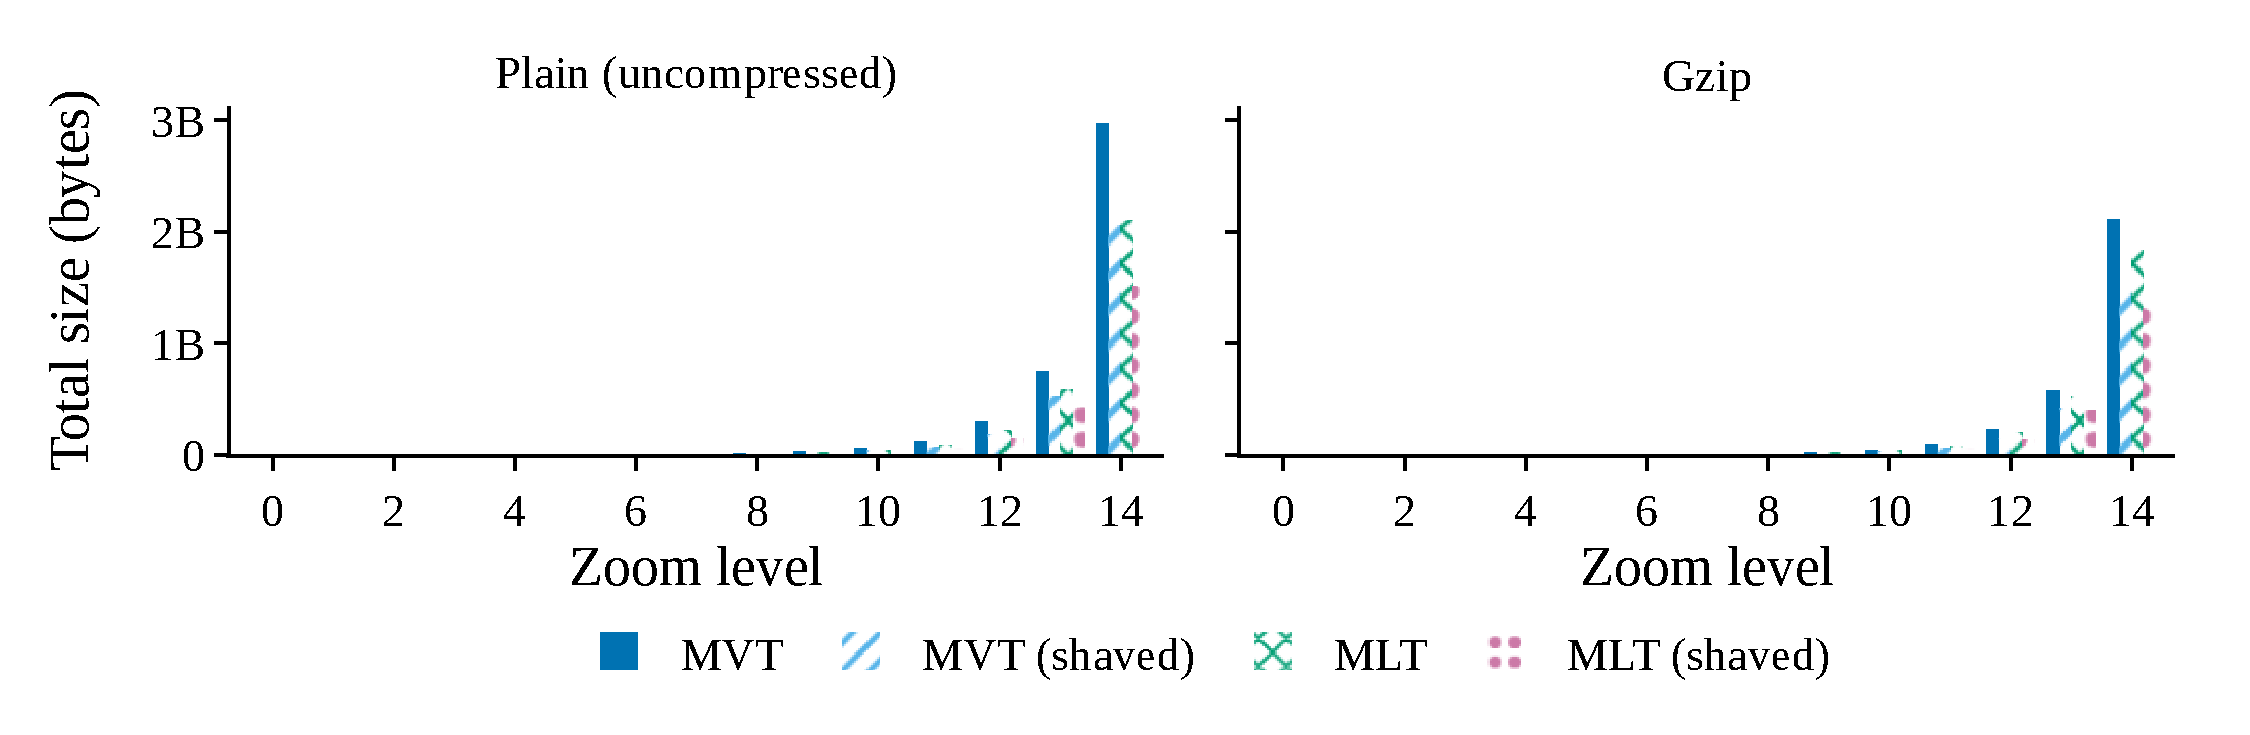
\includegraphics[width=0.9\linewidth]{figures/shaving_effectiveness_per_zoom}
    \caption{
Total tile size per zoom level for unshaved and shaved variants of
      both \ac{MVT} and our \ac{MLT} encoder, using the Liberty advisory.  The gap
      between each format and its shaved counterpart quantifies the data removed
      by the pruning advisory.
The gap between the shaved \ac{MVT} and the
      shaved output of our encoder quantifies the additional contribution of
      columnar encoding}
    \label{fig:shaving_effectiveness_per_zoom}
\end{figure}

\paragraph{Isolating the Contribution of Our Encoder's Strategy Selection}
To separate the contribution of the multi-strategy competition (this work) from that of the \ac{MLT} format as proposed by Tremmel and Zink~\cite{tremmelMapLibreTileNext2025b}, we report in \cref{fig:encoder_comparison} both a per-zoom breakdown and the total encoded size of the Germany OpenMapTiles tileset (zoom~0-14, \num{256588} tiles) under three encoders (\ac{MVT} as the row-oriented protobuf baseline, the reference \ac{MLT} encoder of Tremmel and Zink as the columnar baseline, and our \ac{MLT} encoder with sort-strategy competition, per-stream profiling, and shared-dictionary clustering) and across four wire compressions (none, gzip-9, Brotli-11, zstd-22).

\begin{figure}[htbp]
\centering
    \begin{subfigure}[t]{0.95\linewidth}
        \centering
        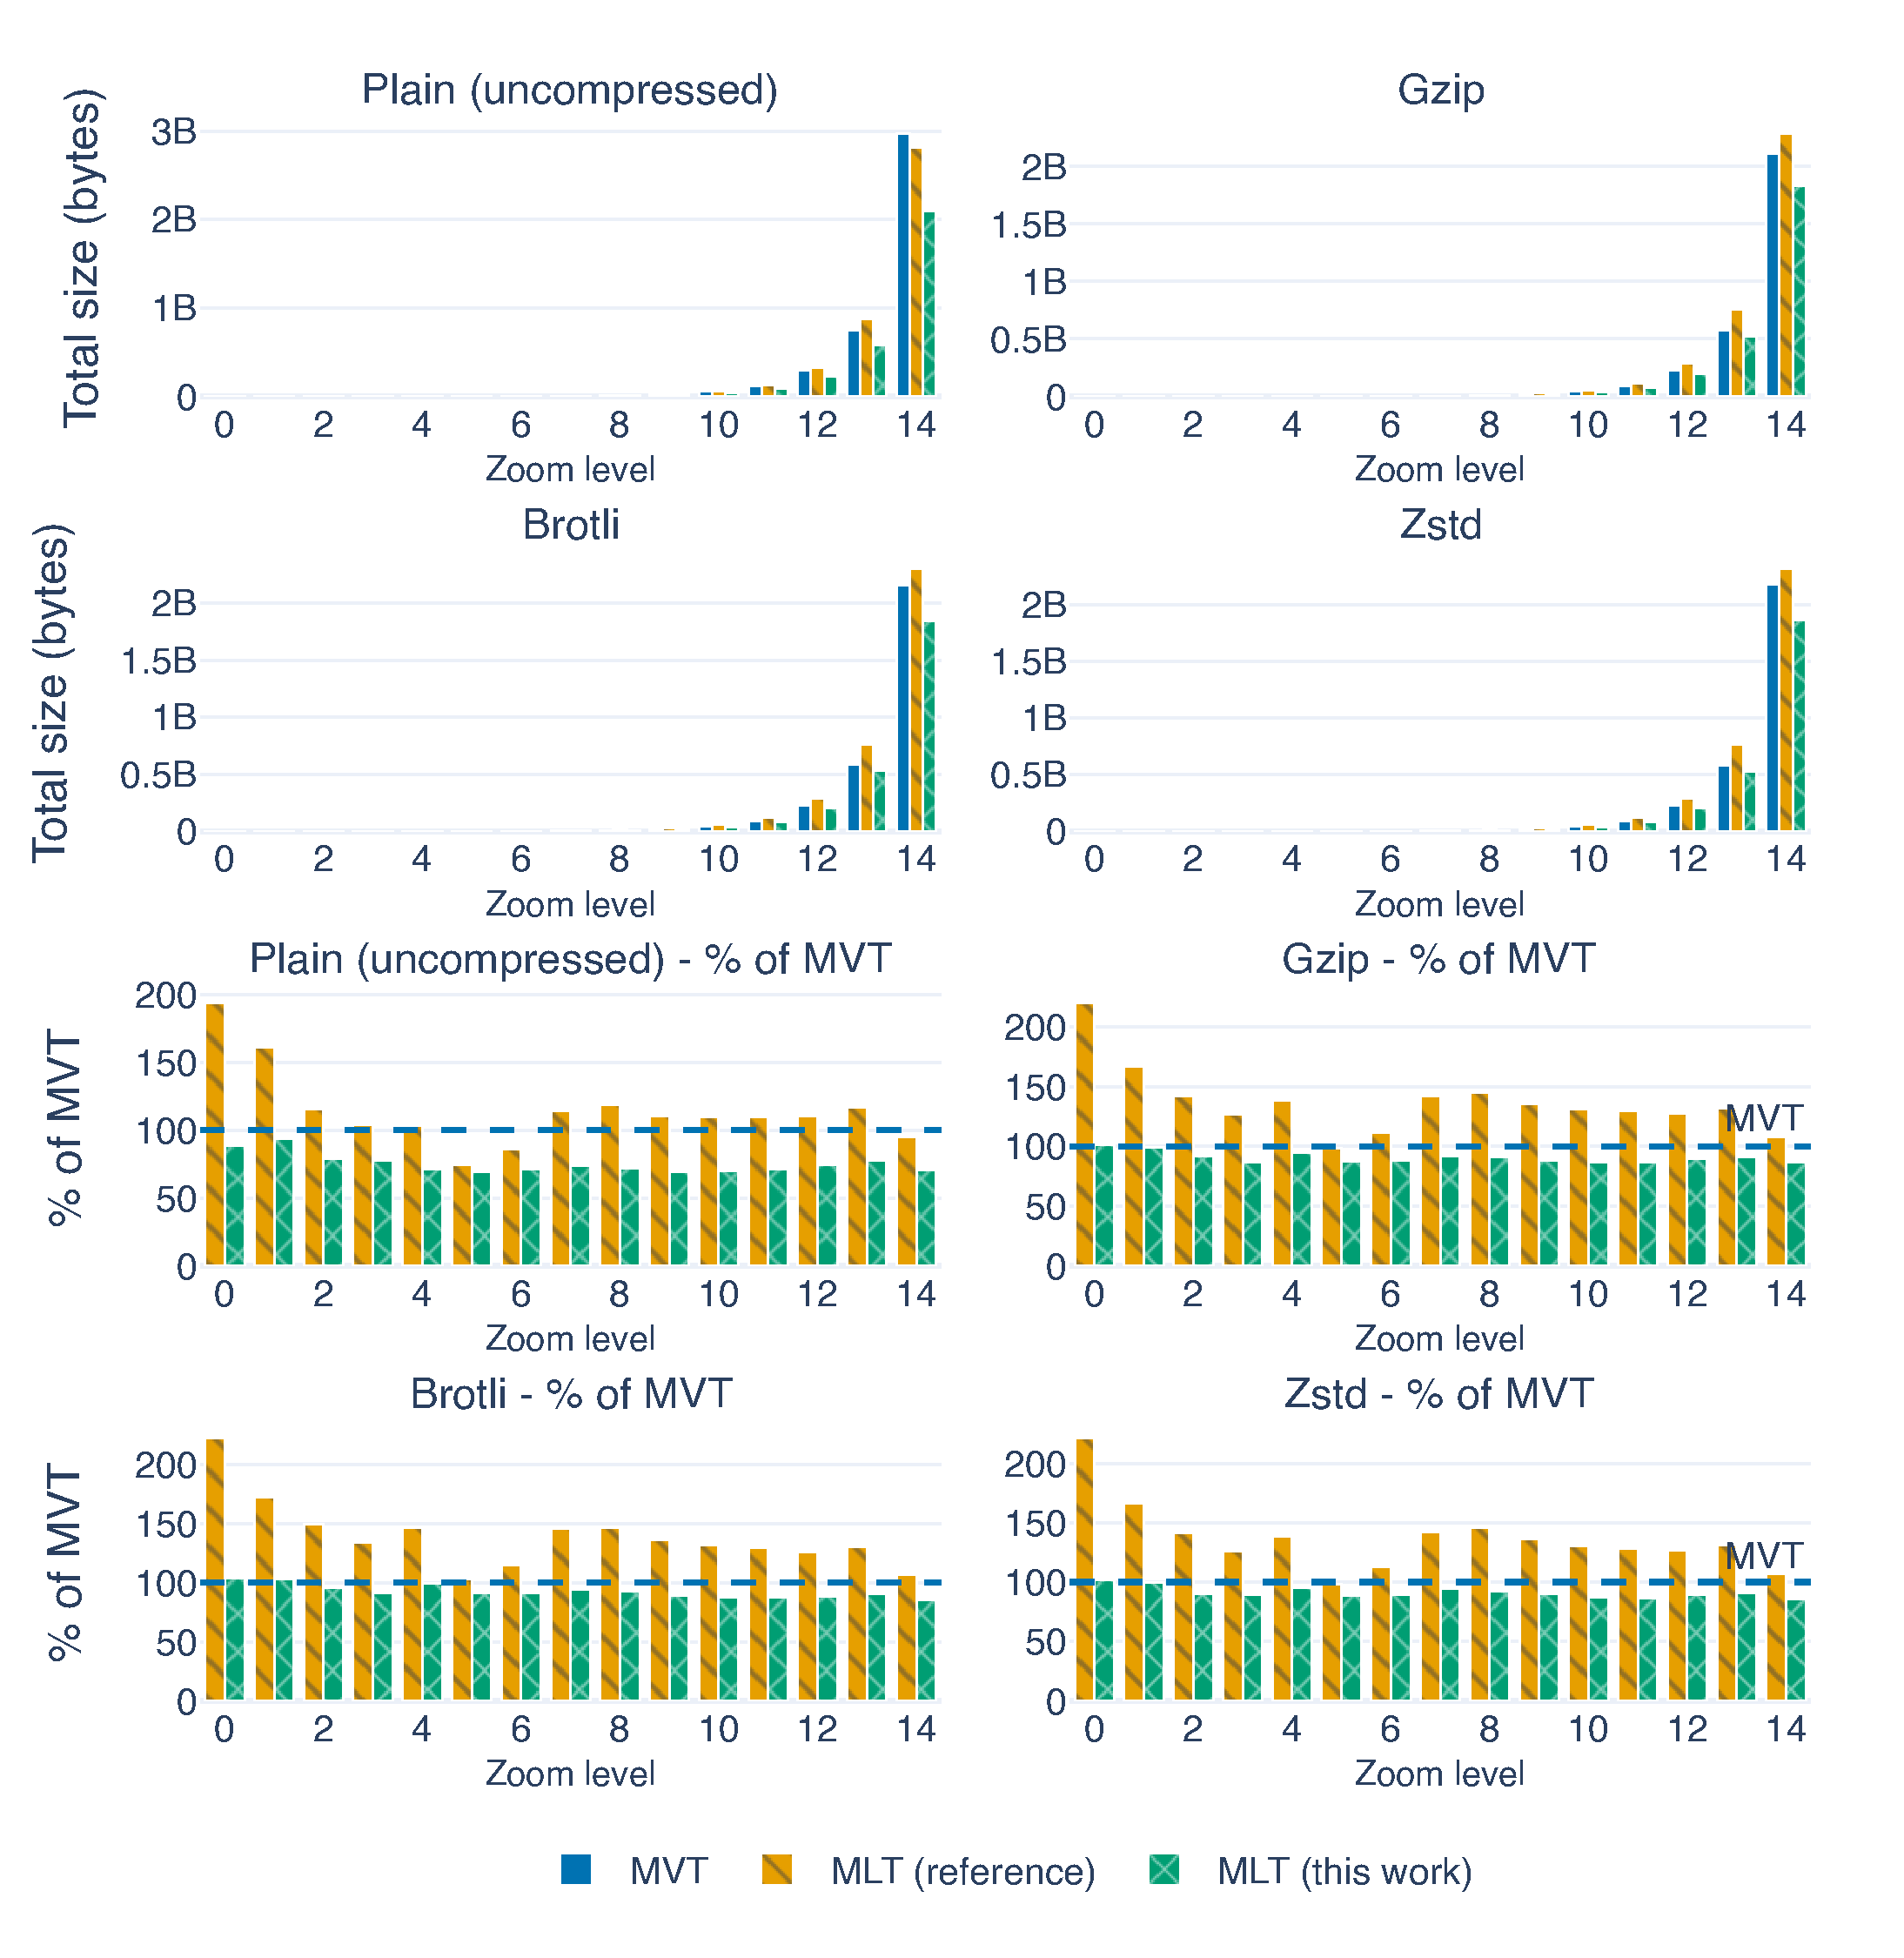
\includegraphics[width=\linewidth]{figures/encoder_comparison_per_zoom}
        \caption{
Per-zoom total tile size for the three encoders under four wire compressions}
        \label{fig:encoder_comparison_per_zoom}
    \end{subfigure}

    \vspace{1em}

    \begin{subfigure}[t]{\linewidth}
        \centering
        \begin{tblr}{colspec={l r r r r}, rows={font=\small}, row{1}={font=\small\bfseries}}
        \toprule
        Encoder & Plain (GB) & gzip (GB) & Brotli (GB) & zstd (GB) \\
        \midrule
        \ac{MVT}              & 4.24 & 3.08 & 3.13 & 3.16 \\
        \ac{MLT} (reference) & 4.26 & 3.54 & 3.57 & 3.60 \\
        \ac{MLT} (this work) & \textbf{3.06} &  \textbf{2.70} &  \textbf{2.72} &  \textbf{2.75} \\
        \midrule
        $\Delta$ ours vs.\ reference & $-28.3\%$ & $-23.8\%$ & $-23.7\%$ & $-23.6\%$ \\
        $\Delta$ ours vs.\ \ac{MVT}  & $-27.9\%$ & $-12.3\%$ & $-13.1\%$ & $-12.9\%$ \\
        \bottomrule
        \end{tblr}
        \caption{
Total tileset size for the three encoders under four wire compressions.
          The \ac{MLT} (reference) column reports the baseline from~\cite{tremmelMapLibreTileNext2025b}, updated with encoding improvements backported from our encoder's development (correct delta-zigzag sequencing, \ac{RLE} viability checks, \ac{FSST} thresholds).
          The \ac{MLT} (this work) column reports the encoder developed in this thesis}
        \label{tab:mvt_mlt_comparison}
    \end{subfigure}
\caption[Encoder comparison: per-zoom breakdown and total tileset size]{Encoder comparison for the Germany OpenMapTiles tileset (zoom~0-14, \num{256588} tiles).
Our \ac{MLT} encoder achieves \qty{28.3}{\percent} smaller total size than the reference baseline under no wire compression.
The reference encoder drifts above \ac{MVT} size at several zoom levels under Brotli/zstd, whereas our encoder remains below \ac{MVT} throughout.}
\label{fig:encoder_comparison}
\end{figure}

The headline is the \qty{28.3}{\percent} reduction our encoder achieves over the reference baseline under no wire compression.
The reference baseline already incorporates encoding fixes backported from our encoder's development (correct delta-zigzag sequencing, \ac{RLE} viability checks, \ac{FSST} thresholds), so the \qty{28}{\percent} isolates the contribution of automatic strategy selection over a correctly-implemented fixed-plan encoder rather than conflating bug fixes with the innovation we want to attribute to.

The finding in the table that is easiest to overlook, and the one we found most uncomfortable when we first plotted it, is that the reference baseline is \emph{worse} than gzip-compressed \ac{MVT} (\qty{3.54}{\giga\byte} vs.\ \qty{3.08}{\giga\byte}).
General-purpose LZ77-family compressors already exploit most of the row-level redundancy in the protobuf wire format, and a columnar encoder that uses fixed per-column schemes cannot keep up.
The data-driven strategy selection in our encoder reclaims this gap and goes past it: our encoder under gzip is \qty{12.3}{\percent} smaller than \ac{MVT} under gzip, and the advantage holds (\qty{12.9}{\percent}) even against zstd-22, the strongest general-purpose compressor in the comparison.

The relative gap between our encoder and the reference is roughly constant across all four compressors (\qty{-23}{\percent} to \qty{-28}{\percent}).
This stability is consistent with the profiler capturing genuine redundancy that general-purpose compressors miss, but it could equally reflect that the profiler removes the same redundancy the compressors would have.
The cleaner evidence for the profiler's value is the absolute comparison: our encoder, uncompressed (\qty{3.06}{\giga\byte}), is already smaller than \ac{MVT}+gzip (\qty{3.08}{\giga\byte}), confirming that per-stream encoding captures type-specific redundancy that LZ77-family compressors miss on the interleaved protobuf byte stream.
This directly answers the question we posed at the start of \cref{sec:exp_mlt}: our encoder's contribution lives in the joint strategy-selection layer that sits on top of the columnar format, not in the format alone.

\paragraph{Scope of the Encoder Contribution}
We measured the \qty{28}{\percent} reduction reported in \cref{tab:mvt_mlt_comparison} on the \emph{unshaved} Germany tileset, so it is an encoder-only improvement, independent of the style-driven optimizations.
It reflects the combined effect of sort-strategy competition, per-stream profiling, and shared-dictionary clustering.
These three mechanisms are tightly coupled (sort order affects column distributions, which affect profiling decisions), so a per-mechanism decomposition is not feasible without re-engineering the encoder.
This result is complementary to, but separate from, the style-data bridge: style-driven tile shaving reduces tile content before encoding, while the encoder improvements reduce the encoded size of whatever content remains.
The two contributions stack (shaved tiles encoded with our encoder are smaller than shaved tiles encoded with the reference baseline), but they address orthogonal sources of redundancy.

\paragraph{zstd-on-\acs{MVT} Comparison}
A natural objection is that general-purpose compressors such as zstd-22 or Brotli-11 should be sufficient: if compression is the goal, simply applying the strongest available compressor to the existing \ac{MVT} wire format would avoid the complexity of a columnar encoder entirely.
\Cref{tab:mvt_mlt_comparison} answers this directly.
\ac{MVT} under zstd-22 yields \qty{3.16}{\giga\byte} for the Germany tileset, whereas our encoder under the same compressor yields \qty{2.75}{\giga\byte}, a \qty{12.9}{\percent} reduction.
We attribute this to a structural difference: a general-purpose compressor sees the interleaved, heterogeneous protobuf byte stream and must discover redundancy across mixed data types.
A columnar encoder, by contrast, groups homogeneous values (all road classes in one stream, all vertex deltas in another) and each stream compresses more effectively under lightweight per-type codecs (delta-\acs{RLE} for monotonic integers, dictionary encoding for low-cardinality strings, \ac{FSST} for high-cardinality strings) than a monolithic LZ77-family compressor can achieve on the interleaved byte stream.
The columnar advantage is preserved \emph{after} applying the same general-purpose compressor on top: the per-column codecs have already removed most of the type-specific redundancy, so the post-hoc compressor has less work to do but starts from a lower baseline.
This finding is consistent with the columnar-database literature, where per-column lightweight encoding consistently outperforms row-level block compression even when the block compressor is state-of-the-art~\cite{kuschewskiBtrBlocksEfficientColumnar2023}.

\paragraph{Decoder Cost}
A legitimate concern for any multi-encoding scheme is that the client must pay the decoder cost, which can erode the transfer savings on mobile or battery-constrained targets.
We engineered the decoder to amortise its per-column dispatch over per-feature work (\cref{sub:encoding_strategies}).
Empirically, our benchmarks on the full Germany tileset show end-to-end rendering metrics comparable to or better than \ac{MVT} at matched workloads, and we see no negative effect in the sustained frame-time metrics of \cref{sub:combined_marginal}.


\paragraph{Decoding Throughput}
To isolate decoding latency from the browser-based rendering benchmark (where it is embedded in \texttt{loadMs}), we use Criterion micro-benchmarks to measure full-decode throughput for our \ac{MLT} decoder vs.\ \ac{MVT} with and without transport compression.
Each benchmark parses the tile header and materialises all features and properties; \ac{MVT} variants include gzip decompression in the measured path.
\Cref{tab:decode_throughput} reports the results on a representative subset of the OpenMapTiles fixture tiles at zoom levels~4, 7, and~13 (100~samples per cell).

\begin{table}[htbp]
\centering
\small
\begin{tblr}{colspec={l r r r}, rows={font=\small}, row{1}={font=\small\bfseries}}
\toprule
Format & Zoom~4 & Zoom~7 & Zoom~13 \\
\midrule
\ac{MLT} (this work) & \qty{5.73}{\milli\second} & \qty{19.4}{\milli\second} & \qty{4.09}{\milli\second} \\
\ac{MVT}+gzip & \qty{47.6}{\milli\second} & \qty{103}{\milli\second} & \qty{18.7}{\milli\second} \\
\ac{MVT} (uncompressed) & \qty{44.2}{\milli\second} & \qty{90.6}{\milli\second} & \qty{16.5}{\milli\second} \\
\midrule
Speedup (vs.\ gzip) & $8.3\times$ & $5.3\times$ & $4.6\times$ \\
\bottomrule
\end{tblr}
\caption{
Full-decode latency for our \ac{MLT} decoder vs.\ \ac{MVT} on OpenMapTiles fixture tiles, measured by Criterion micro-benchmarks (100~samples per cell).
Our decoder achieves \numrange{96}{134}\,MiB/s decode throughput vs.\ \numrange{15}{23}\,MiB/s for \ac{MVT}+gzip (measured over wire-format input size)}
\label{tab:decode_throughput}
\end{table}

The \ac{MLT} decoder's columnar layout enables selective column access and avoids the per-feature tag-parsing overhead of protobuf, which accounts for the speedup even before transport decompression is considered: our decoder is $4.0$-$7.7\times$ faster than uncompressed \ac{MVT}.
These micro-benchmark results complement the browser-based \texttt{loadMs} metric by providing an isolated measurement of the decoding-latency axis of Research Goal~R3, even though they are not 1:1 applicable because we do not use our decoder in \texttt{maplibre-gl-js}.

\subsection{Discussion}\label{sub:mlt_discussion}

Tile shaving alone cuts pooled median load time by \qty{71.5}{\percent} and lifts \ac{FPS} by \qty{184}{\percent}, while style-only passes contribute \qty{-4.1}{\percent} on load.
The two channels compose additively, not synergistically.
We discuss why the channels stay additive, the cache-fragmentation trade-off that style-dependent tiles create on shared \acsp{CDN}, and the geometry-simplification axis we leave out of scope.

\paragraph{Dominance of Tile Shaving and Additive Style-Pass Contribution}
The headline finding of this experiment is that tile shaving is the dominant contributor to load-time and transfer-size improvements, while style-level passes provide a modest, additive assist.
Dead layer elimination (Experiment~2) removes style layers whose filters are unsatisfiable.
Each removed layer reduces the set of referenced properties in the pruning advisory, which in turn can eliminate columns from the encoded tile.
Metadata refinement tightens zoom bounds, which causes the advisory to mark additional zoom levels as unused, potentially eliminating tiles entirely.
However, the aggregate data shows no super-additive interaction at the median level (\cref{sub:mlt_results}): the combined style+shaving reduction is approximately the sum of the individual reductions, not greater.
We therefore best understand the style-level passes as useful enablers (simplifying the advisory and improving code quality) rather than as co-equal partners in a synergistic cascade.
The encoding stage that follows benefits from this enabling effect: shaved data presents longer runs and smaller dictionaries to the per-stream profiler, which is why we place the multi-strategy competition in the same pipeline rather than as a standalone encoder paper.

\paragraph{Style-Dependent Tile Sizes}
A consequence of style-driven shaving is that different styles produce different tile sizes from the same source data.
To quantify this variation, we ran the full shaving pipeline (optimize with all passes, generate pruning advisory, apply advisory as \ac{MVT}) on the same Germany tileset (\qty{3.07}{\giga\byte}, OpenMapTiles schema, zoom levels 0-14) for each of the 11 \ac{OMT}-compatible styles in the benchmark corpus.
\cref{fig:tile_shave_per_style} shows the results: tile-data reductions range from \qty{19.8}{\percent} (Bright) to \qty{46.3}{\percent} (Toner), with a median of \qty{29.0}{\percent}.
Styles that reference fewer source-layers and property columns (such as Toner with monochrome road/water/boundary only and Americana focused on shield and label rendering) leave more tile data unused, enabling the advisory to strip more columns and features.
Conversely, broad-coverage styles like Bright and OSM~Bright reference most of the tileset's property columns, limiting the shaving headroom.
We see this observation as highlighting a fundamental trade-off: there is no single optimal tile.
The optimal encoding depends on the rendering style, which is a design choice.

\begin{figure}[htbp]
    \centering
    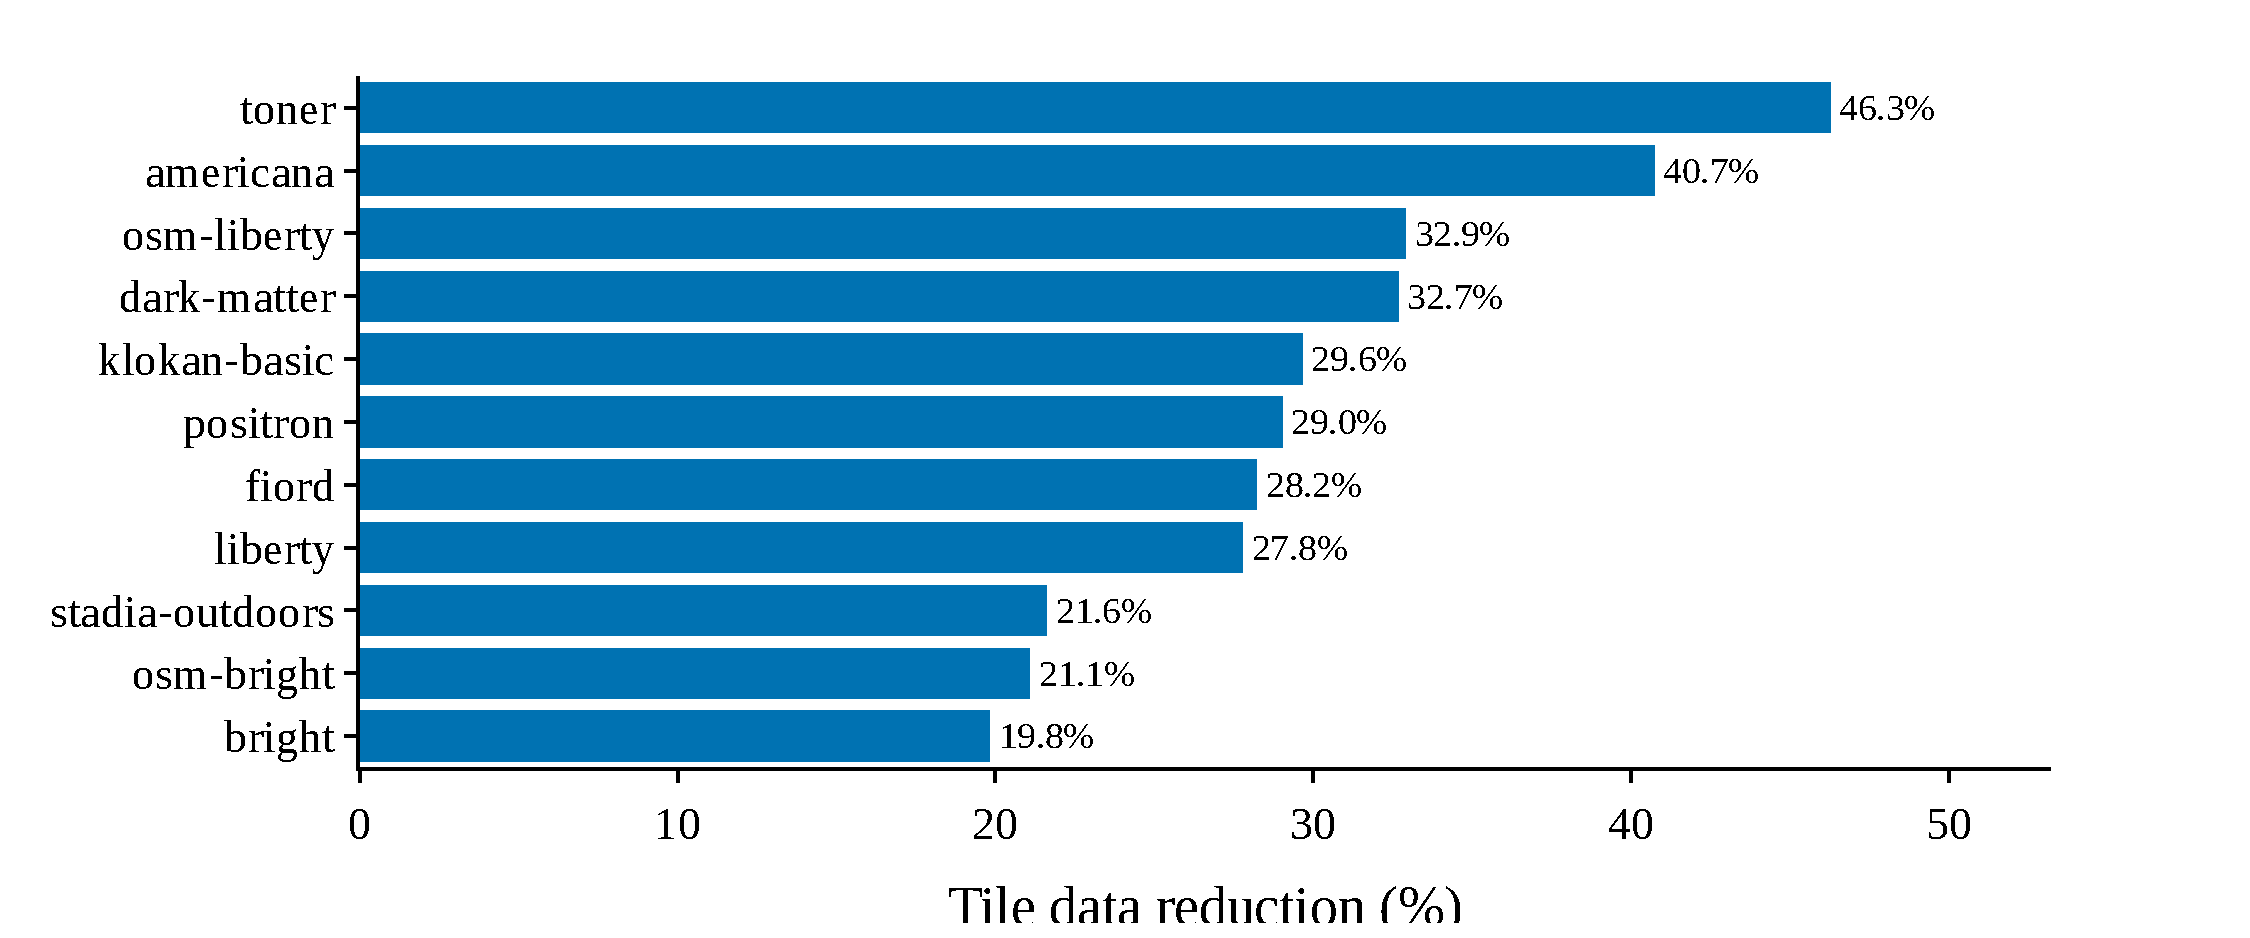
\includegraphics[width=0.8\linewidth]{figures/tile_shave_per_style}
    \caption{
On-Wire data reduction from style-driven \ac{MVT} shaving across 11 \ac{OMT}-compatible styles, applied to the same \qty{3.07}{\giga\byte} Germany tileset.  Styles that reference fewer source-layers and properties achieve larger reductions}
    \label{fig:tile_shave_per_style}
\end{figure}

\paragraph{Cache Fragmentation Trade-Off}
A direct operational consequence of style-dependent tiles is that shared \ac{CDN} caching is partially defeated.
Two styles that served identical tiles under \ac{MVT} now fetch distinct shaved variants, and a \ac{CDN} must either key its cache on (tile, style) pairs or accept that a hit on one style is a miss on another.
For deployments where a single style dominates traffic, style-driven shaving is strictly beneficial.
For multi-tenant tile servers hosting dozens of styles, operators should apply shaving per style and cache the resulting tile variants independently (the approach of Mapbox's closed-source \enquote{style-optimized vector tiles} service~\cite{StyleoptimizedVectorTiles}).

We frame the decision with a per-style break-even model.
A vector-tile source's \texttt{encoding} field selects \ac{MVT} or \ac{MLT}, so the two formats cannot mix within one source.
Unshaved \ac{MLT} is possible in principle but not emitted by our tool, so each style is served either as shaved \ac{MLT} (with its own \emph{(tile, style)} cache-key namespace) or as raw \ac{MVT} (sharing cache slots with all other \ac{MVT}-served styles).
The choice is usually binary per style (given most styles only have one vector tile source), and the operational question is which styles belong in which group.

Let $r$ denote the per-tile rendering-time saving from shaving (load-time reduction divided by the number of fetched tiles), $C_f$ the origin fetch cost per cache miss, $\lambda_i$ the aggregate request rate to style $i$, $N$ the number of distinct tiles, and $\mathcal{M}$ the subset of styles served as \ac{MVT} with pooled rate $\Lambda_\mathcal{M} = \sum_{i \in \mathcal{M}} \lambda_i$.
Let $h(\mu)$ denote the steady-state hit rate of a cache slot accessed at rate $\mu$ on the shared edge cache.
Under \ac{LRU}, $h$ is monotonically increasing in $\mu$ and saturates near $1$ for popular content.
A style-$j \in \mathcal{M}$ request hits the per-tile pooled slot at rate $\Lambda_\mathcal{M}/N$, while a style served as shaved \ac{MLT} hits its own \emph{(tile, style)} slot at rate only $\lambda_i/N$.
Moving style $i$ from $\mathcal{M}$ to the \ac{MLT}-served set is net-beneficial when
\[
    r \;>\; \big[\, h(\Lambda_\mathcal{M}/N) - h(\lambda_i/N) \,\big] \cdot C_f
\]
where the bracketed \emph{hit-rate gap} measures the cache warmth that style $i$ surrenders by leaving the pool.
The decision depends on style $i$'s share of pool traffic, not on the total number of styles served.

We identify two practically meaningful regimes.
A \emph{dominant style} ($\lambda_i$ comparable to $\Lambda_\mathcal{M}$) sees a near-zero gap, since the pool was already warmed almost entirely by its own traffic, and any positive $r$ justifies shaving.
A \emph{long-tail style} ($\lambda_i \ll \Lambda_\mathcal{M}$) sees a gap that approaches the full pooled hit rate $h(\Lambda_\mathcal{M}/N)$, because its private cache cannot self-warm on its own thin traffic and reverts to near-cold-start behavior.
With our benchmark values ($r \approx \qty{3}{\milli\second}$ per tile, $C_f \approx \qty{25.8}{\milli\second}$ under the Rusan et al.~\cite{rusanAssessmentPacketLatency2015} $\frac{\text{tile size}}{\qty{30}{\mega\bit\per\second}} + \frac{\qty{25}{\milli\second}}{2}$ server-side-throttle for a \qty{50}{\kilo\byte} average tile) and a representative pooled hit rate $h(\Lambda_\mathcal{M}/N) \approx 0.9$ for popular tile content, the maximum tolerable hit-rate gap is $r/C_f \approx 11.6\%$.

Under typical \ac{LRU} dynamics this in turn requires the style to hold a majority share of pool traffic before it can be shaved profitably.
We draw the corollary of the hybrid pattern from this:
shave the one or two canonical styles that dominate the pool, and leave the long tail on raw \ac{MVT}.
Traffic concentration drives this recommendation, not style count.
A server hosting fifty styles with one \qty{70}{\percent}-share dominant style behaves the same as one hosting five with the same concentration.
Our model omits spatial locality and the second-order effect that peeling the dominant style off the pool cools the cache further for the remaining \ac{MVT}-served styles, both of which would only sharpen the recommendation.

\paragraph{Geometry Simplification as out of scope}
A complementary direction we do not explore in this thesis is geometry-level pruning - coordinate precision reduction, Visvalingam~\cite{visvalingamLineGeneralisationRepeated1993} or Douglas-Peucker~\cite{douglasALGORITHMSREDUCTIONNUMBER1973} simplification, and polygon topology coalescing - which is the principal lever used by upstream generators such as Tippecanoe\footnote{\url{https://github.com/felt/tippecanoe}, last accessed 2026-04-21} and Planetiler\footnote{\url{https://github.com/onthegomap/planetiler}, last accessed 2026-04-21}.
These techniques typically deliver larger absolute savings than attribute-column pruning, but they interact non-trivially with style-defined visual thresholds (line width, dash pattern length, label anchor placement) and would violate the pixel-identity soundness criterion established in \cref{sec:problem_statement}.
Style-driven geometry simplification, choosing a simplification tolerance that is demonstrably below the smallest visible feature at each zoom level, is an interesting direction for future work but we do not pursue it here.
We therefore quantify the size reductions achievable \emph{without} touching geometry at all, which understates the total optimizations headroom a production pipeline could reach by composing this work with an upstream simplifier.

\section{Cross-Style Generalisation}\label{sec:exp_cross_style}
\begin{keytakeaways}
\item Static-only passes generalize: median \qty{31.4}{\percent} raw reduction across 13 unseen styles, none regressed.
\item Initial style size and complexity does not predict reduction ($r = 0.35$, $n = 13$, $p = 0.24$).
\item These numbers are a lower bound.
Stats-driven and data-level passes were not applied here.
\end{keytakeaways}

\noindent In the preceding experiments we evaluated optimizations effectiveness on the curated benchmarking corpus of 15 styles described in \cref{sub:deep_corpus}.
To assess whether the observed gains generalize, we apply the optimizer to the 13~styles of the Maputnik generalization corpus introduced in \cref{sub:generalization_corpus}.
We use three tiers of breadth because end-to-end rendering benchmarks require tile data and browser automation infrastructure that does not scale to all styles: we benchmark ten deep-corpus styles end-to-end with tile data, eleven \ac{OMT}-compatible styles at the tile-shaving size level, and evaluate thirteen additional styles with static analysis only.

\subsection{Methodology}\label{sub:cross_methodology}

We use static analysis only for the cross-style evaluation: we optimize each style with all passes enabled, and compare the resulting style to the original on size and complexity metrics.
We execute no rendering benchmarks, as the diverse styles reference incompatible tile schemas and tile sources that we cannot uniformly provision.

\subsection{Results}\label{sub:cross_results}

\cref{fig:cross_style_reduction} shows per-style percentage reductions (raw, gzip, Brotli) across the 13 Maputnik styles, sorted by raw reduction.
The key question here is whether the distribution clusters tightly around the deep corpus median or fans out with substantial per-style variance.
\cref{fig:cross_style_complexity_scatter} then plots each style's initial complexity against its achievable reduction, testing the hypothesis that verbose institutional styles (the right-hand side of the scatter) have disproportionately more optimizations headroom than already-compact minimal basemaps on the left.

The distribution fans out considerably:
raw reductions range from \qty{3.2}{\percent} (Stadia Outdoors) to \qty{67.7}{\percent} (LocationIQ Streets), with no style regressing.
Under gzip compression the range narrows to \qtyrange{3.9}{22.4}{\percent} (median \qty{11.4}{\percent}), confirming that some of the raw-byte savings overlap with what gzip already captures.
The top reducers (LocationIQ Streets at \qty{67.7}{\percent} raw, Americana at \qty{59.2}{\percent}, and MapTiler Toner at \qty{57.5}{\percent}) are styles with either verbose filter logic (LocationIQ, Americana) or highly repetitive property structures (Toner).
At the low end, Stadia Outdoors (\qty{3.2}{\percent}) and the two AWS styles (both at \qty{10.6}{\percent}) leave little for the optimizer to remove: the AWS pair shares a codebase of hand-tuned expressions with few redundancies, while Stadia Outdoors is a compact, already-minified basemap.
We observe no statistically significant correlation between initial \ac{AST} node count and reduction ($r = 0.35$, $n = 13$, $p = 0.24$).
The sample size is too small for this correlation to be meaningful.  Americana has by far the highest initial complexity (\num{48510} nodes) and is also one of the top three reducers, but it is a single high-leverage point: dropping it flips the sign to $r = -0.54$, underscoring that no stable trend exists at this sample size.

\begin{figure}[htbp]
    \centering
    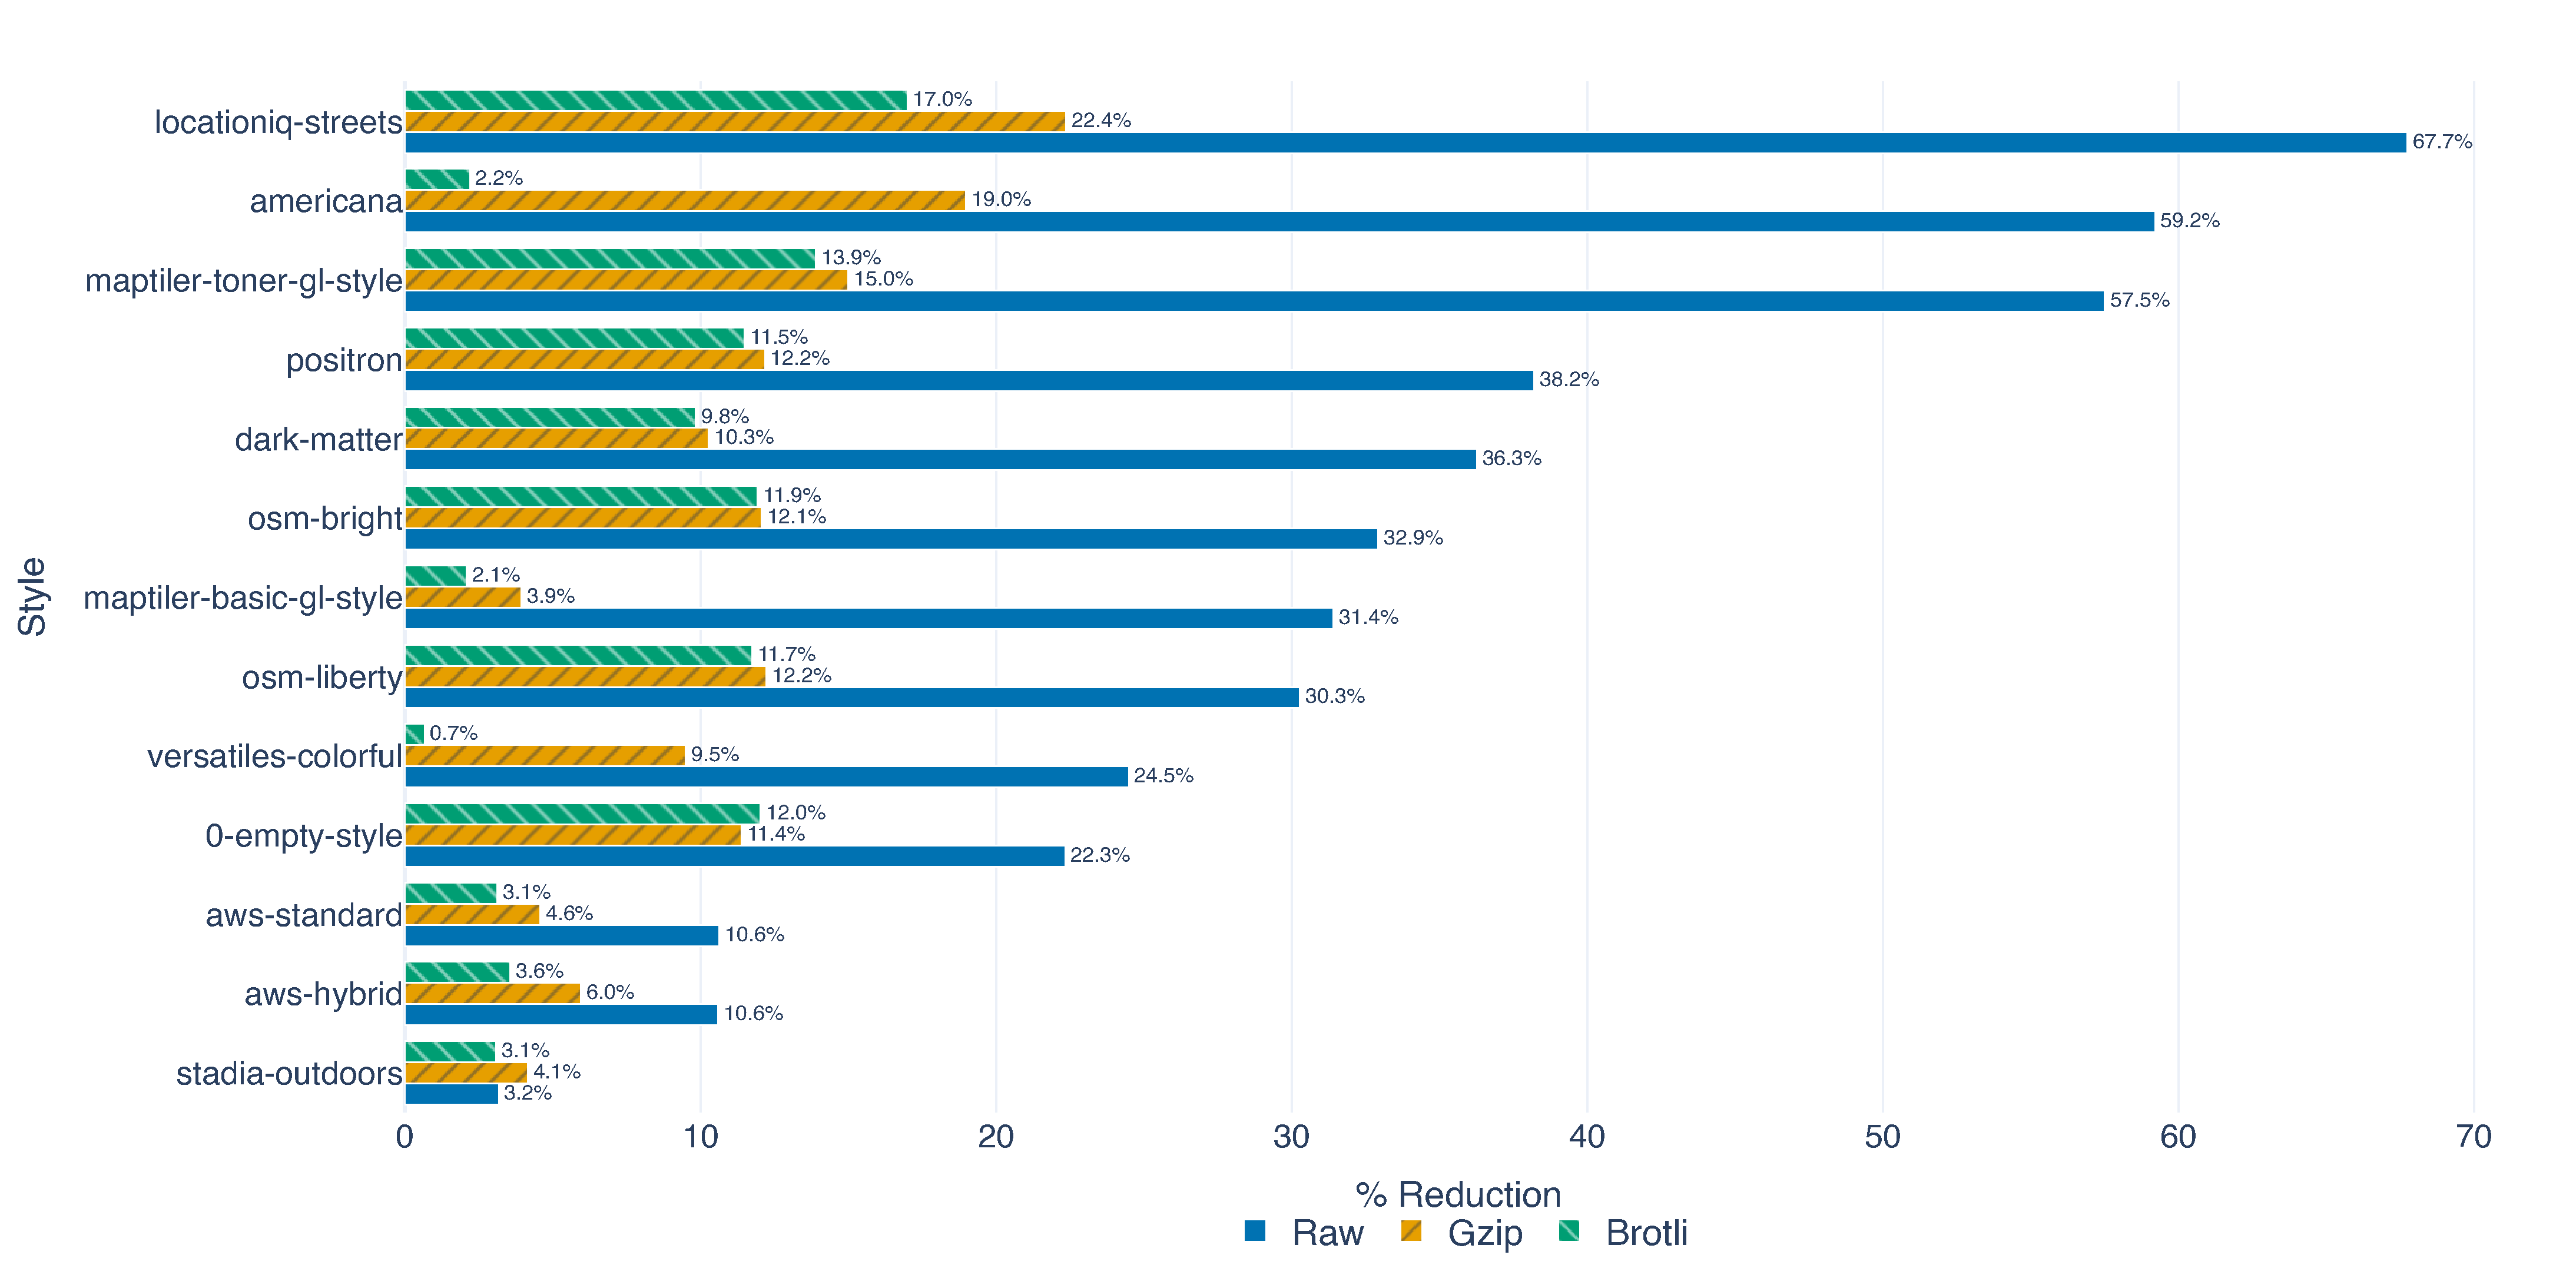
\includegraphics[width=\linewidth]{figures/cross_style_reduction.pdf}
    \caption{
Per-style percentage reduction in style size (raw, gzip, Brotli) across the Maputnik generalization corpus, with styles sorted by raw reduction.
Raw reductions range from \qty{3.2}{\percent} to \qty{67.7}{\percent}, confirming that automatic optimization yields meaningful gains across styles regardless of origin.}
    \label{fig:cross_style_reduction}
\end{figure}

\begin{figure}[htbp]
    \centering
    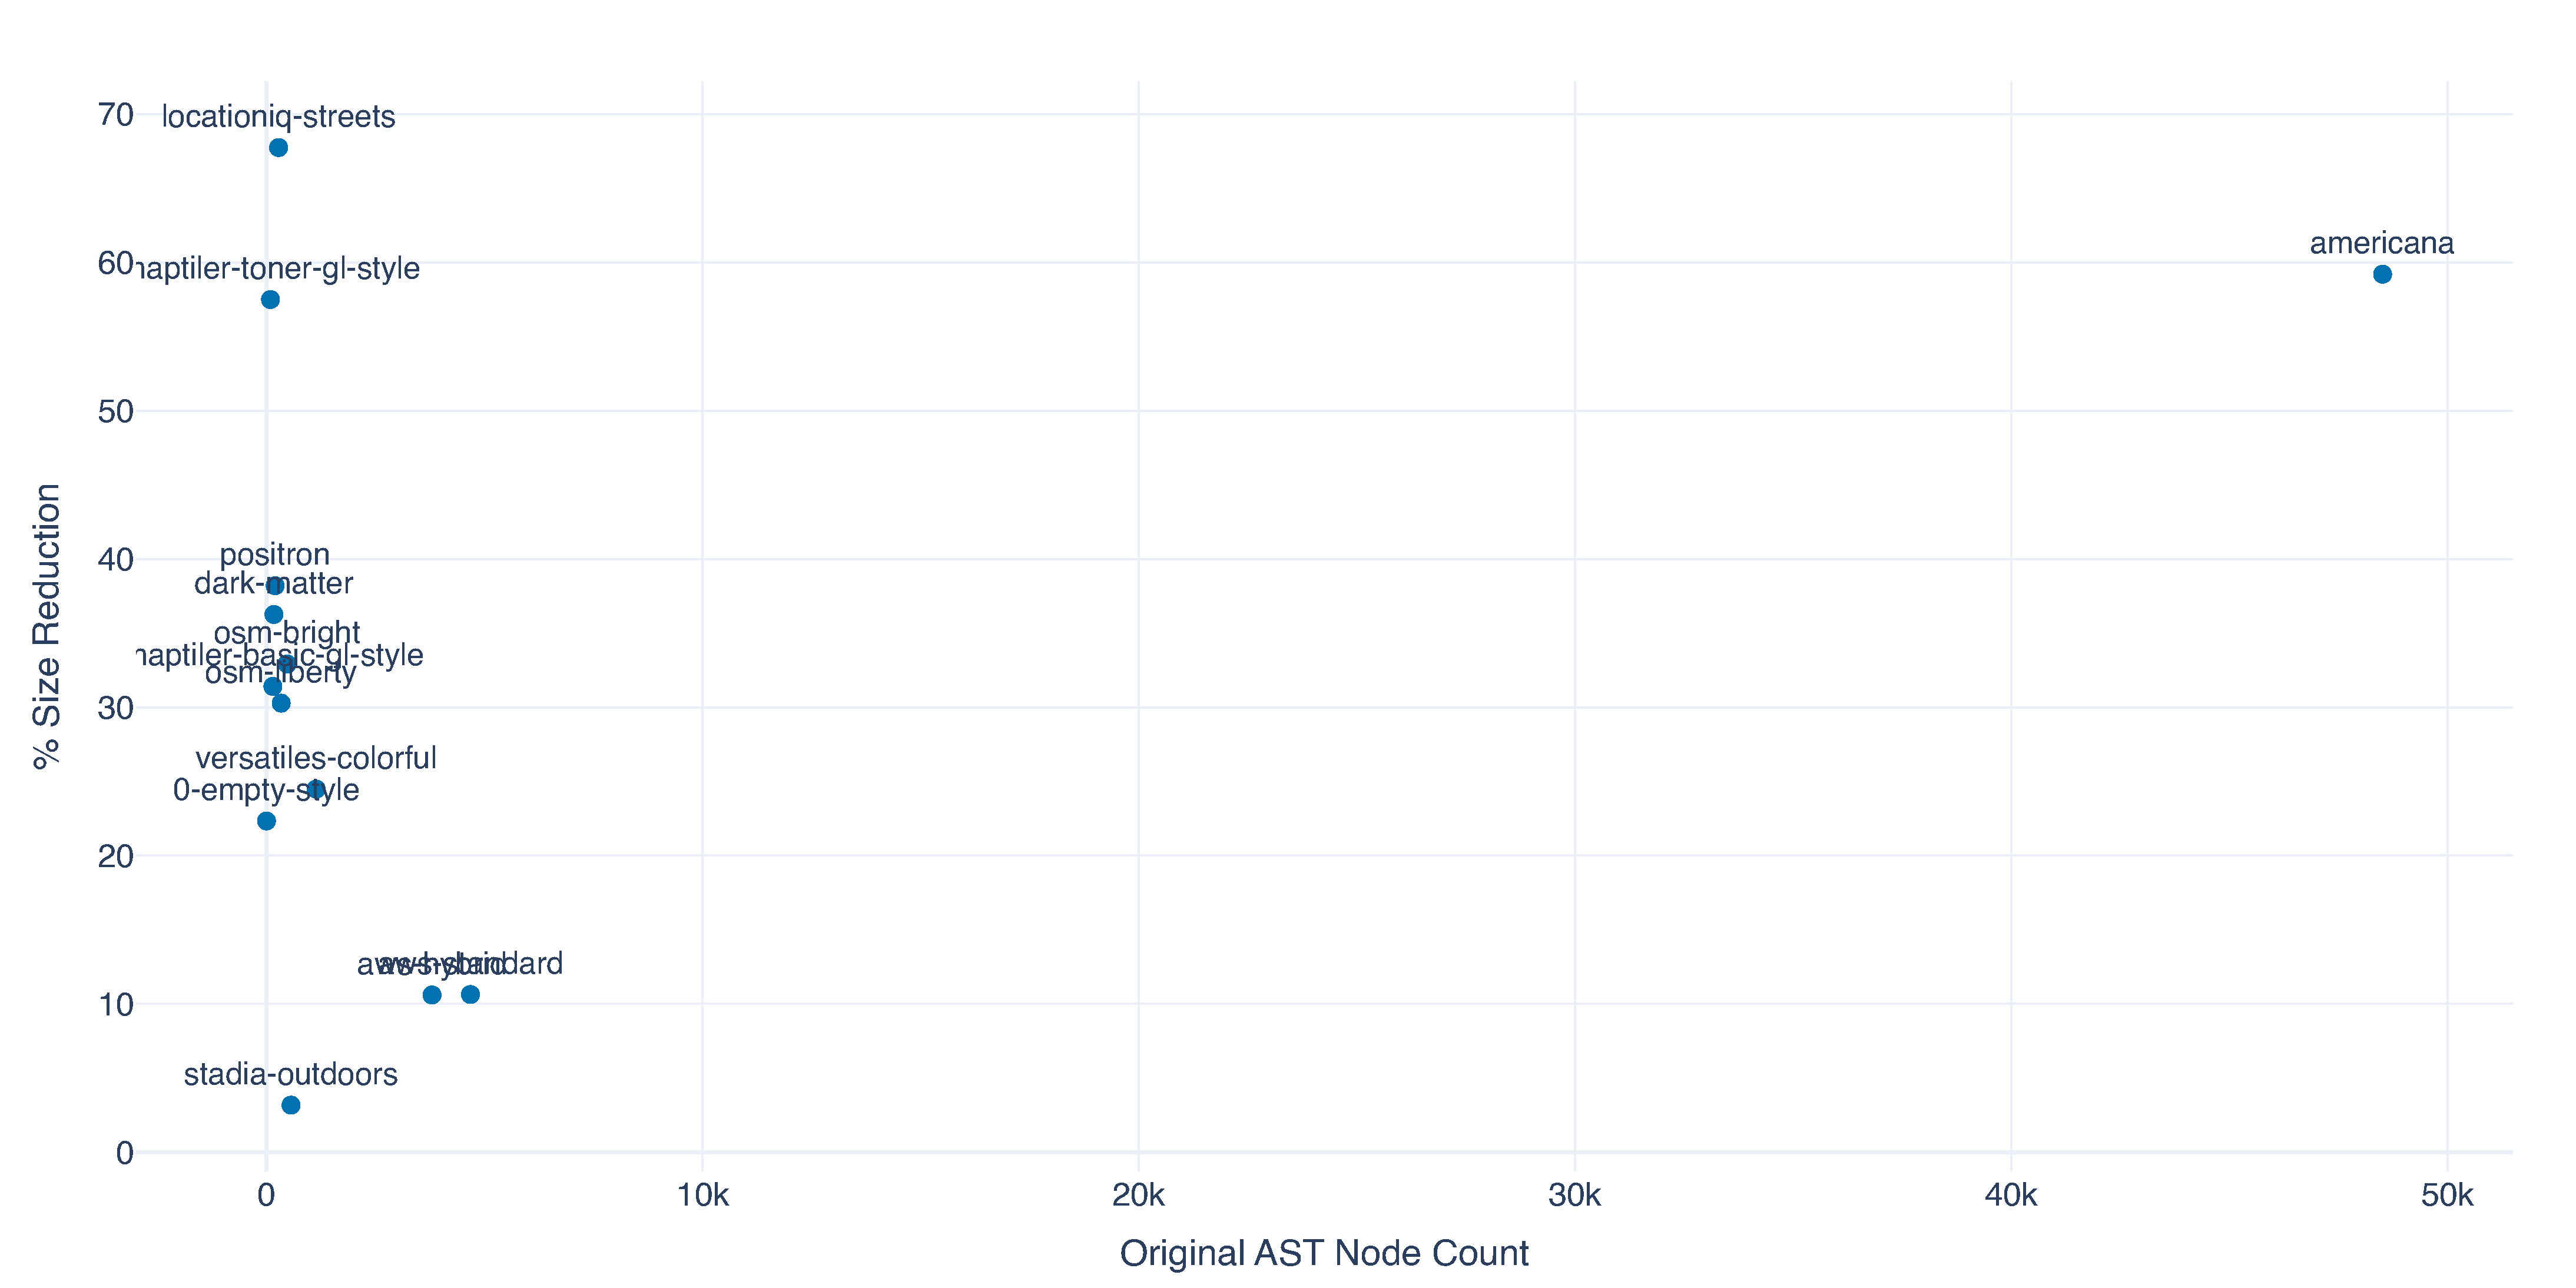
\includegraphics[width=\linewidth]{figures/cross_style_complexity_scatter.pdf}
    \caption{
Relationship between initial style complexity (\ac{AST} node count) and achievable raw style size reduction across the Maputnik generalization corpus.
The correlation is not statistically significant ($r = 0.35$, $n = 13$, $p = 0.24$), and is driven by a single high-leverage point (Americana).
Dropping it flips the sign to $r = -0.54$.
Optimization yield is therefore not reliably predictable from complexity alone, but a combination of other factors such as the cartographers' skill.}
    \label{fig:cross_style_complexity_scatter}
\end{figure}

\begin{table}[htbp]
\centering
\small
\begin{tabular}{l r r r r r}
\toprule
\textbf{Metric} & \textbf{Min} & \textbf{P25} & \textbf{Median} & \textbf{P75} & \textbf{Max} \\
\midrule
Raw size reduction (\%)         &    3.2 &   22.3 &  31.4 & 38.2 & 67.7 \\
Gzip size reduction (\%)        &    3.9 &    6.0 &  11.4 & 12.2 & 22.4 \\
Brotli size reduction (\%)      &    0.7 &    3.1 &   9.8 & 11.9 & 17.0 \\
Layer count reduction (\%)      &    0.0 &    0.8 &   4.8 &  7.0 & 27.0 \\
\ac{AST} node count change (\%) & $-269.2$ & $-102.9$ & $-47.9$ & 0.0 & 62.2 \\
\bottomrule
\end{tabular}
\caption{
Distribution of style-size and complexity changes across the Maputnik generalization corpus (13 styles, static passes only).
Median raw reduction is \qty{31.4}{\percent} and median Brotli reduction is \qty{9.8}{\percent}.
The \ac{AST}-node row is signed: positive values denote a reduction in node count, negative values denote growth from expression rewriting (e.g.\ unrolling \texttt{match} into nested \texttt{case}).
Only three of the 13 styles see a net node-count reduction, indicating that the byte-size gains come predominantly from style-level passes (default stripping, layer merging, metadata stripping) rather than from expression simplification alone.}
\label{tab:cross_style_summary}
\end{table}

\subsection{Discussion}\label{sub:cross_discussion}

The static passes deliver a median raw reduction of \qty{31.4}{\percent} (range \qtyrange{3.2}{67.7}{\percent}) across the 13 unseen Maputnik styles, with no style regressing and only a weak link between initial complexity and achievable reduction ($r = 0.35$, $p = 0.24$).
We discuss which pass families generalize universally, why we read these numbers as a lower bound on the full potential, and what the low-reduction edge cases look like in practice.

\paragraph{Universality of Expression Passes}
Expression-level passes (constant folding, boolean simplification, default stripping) produce non-zero reductions for virtually every style in the corpus, regardless of its complexity or tile schema.
We expect this: any style written by a human or generated by an editor is likely to contain at least some redundant expressions, default-valued properties, or suboptimal color encodings.

\paragraph{Complexity and Reduction}
While verbose institutional styles with several hundred layers and deeply nested expressions tend to offer more room for improvement than simple styles with fewer than 50 layers, we find that the correlation between initial style complexity and achievable reduction is not statistically significant at this sample size ($r = 0.35$, $n = 13$, $p = 0.24$), and is dominated by a single high-leverage point.
The scatter plot (\cref{fig:cross_style_complexity_scatter}) visualizes the per-style relationship.

\paragraph{Unevaluated Stats-Dependent Passes}
Because the generalization corpus does not include tile data, we cannot apply stats-driven passes (dead elimination with geometry-type matching, stats-driven constant folding, selectivity reordering) and data-level optimizations (tile shaving, re-encoding) to the Maputnik styles.
We therefore present the reported reductions as a \emph{lower bound} on the full optimizations potential.
Extrapolating from the deep corpus, where stats-driven passes add \qtyrange{10}{20}{\percent} additional reduction on top of static passes, the true optimizations potential for these styles is likely higher.
For the 11 \ac{OMT}-compatible styles in the deep corpus, we evaluated tile shaving separately against the Germany tileset (\cref{fig:tile_shave_per_style}), confirming that data-level reductions generalize across styles.

\paragraph{Edge Cases}
A small number of styles in the corpus show small reductions ($< 5\%$), the lowest being Stadia Outdoors at \qty{3.2}{\percent}.
These are typically minimal styles that already use only literal values (no expressions), have few layers, and do not set properties to their default values.
We observe no style in the corpus that shows a size \emph{increase} after optimizations, confirming that the passes are safe in the general case.
In practice, styles maintained by large organizations (which tend to accumulate verbose filters, redundant default values, and deeply nested expressions over successive authoring iterations) offer the most room for automatic simplification.
Compact basemaps authored by experienced cartographers, which already use efficient expressions and few layers, show correspondingly smaller gains.


\section{Combined Results}\label{sec:exp_combined}
\begin{keytakeaways}
\item The three optimization channels compose additively, not synergistically.
\item Data-level passes do almost nothing for sustained frame rate.
Their lever is load time.
\item No single pass dominates across styles.
The multi-pass design is what generalizes.
\end{keytakeaways}

\noindent This section presents the full pipeline ablation across all 19 cumulative steps (\cref{sub:ablation}) and analyses interactions between expression, structural, and data passes.
The combined view matters because the three categories \emph{can} interact in principle.
Style-level dead elimination narrows tile pruning advisories, and metadata refinement enables more aggressive zoom-stop pruning downstream.

\subsection{Full Pipeline Ablation}\label{sub:combined_ablation}

\cref{fig:heatmap_loadMs} presents the full scenario$\times$step load-time heatmap.
Load-time improvements are unevenly distributed across scenarios: urban, tile-dense scenarios (New York, Tokyo, Paris) show larger absolute improvements than sparse scenarios (Sahara, Amazon), because the tile-fetch component of load time dominates in dense areas.
Expression passes (steps~1-7) produce a diffuse, moderate improvement across most scenarios, whereas the improvement from structural passes (steps~8-15) is concentrated in the few styles and scenarios where dead elimination or layer merging applies.
\cref{fig:heatmap_fps} shows the companion \ac{FPS} view: the gain is broadly aligned with the load-time pattern but lands more uniformly across scenarios, because once tiles are decoded the sustained frame rate is driven by per-feature evaluation cost rather than by tile-fetch latency.

The frame-time consistency metric in \cref{fig:heatmapjankcount} worsens across the ablation as sustained frame rates push past 2000\,\ac{FPS}, where small \ac{GC}-pauses register as proportionally large outliers.
On real consumer hardware capped well below that rate the same pauses would not cross the jank threshold (see caption).

\begin{figure}[htbp]
	\centering
	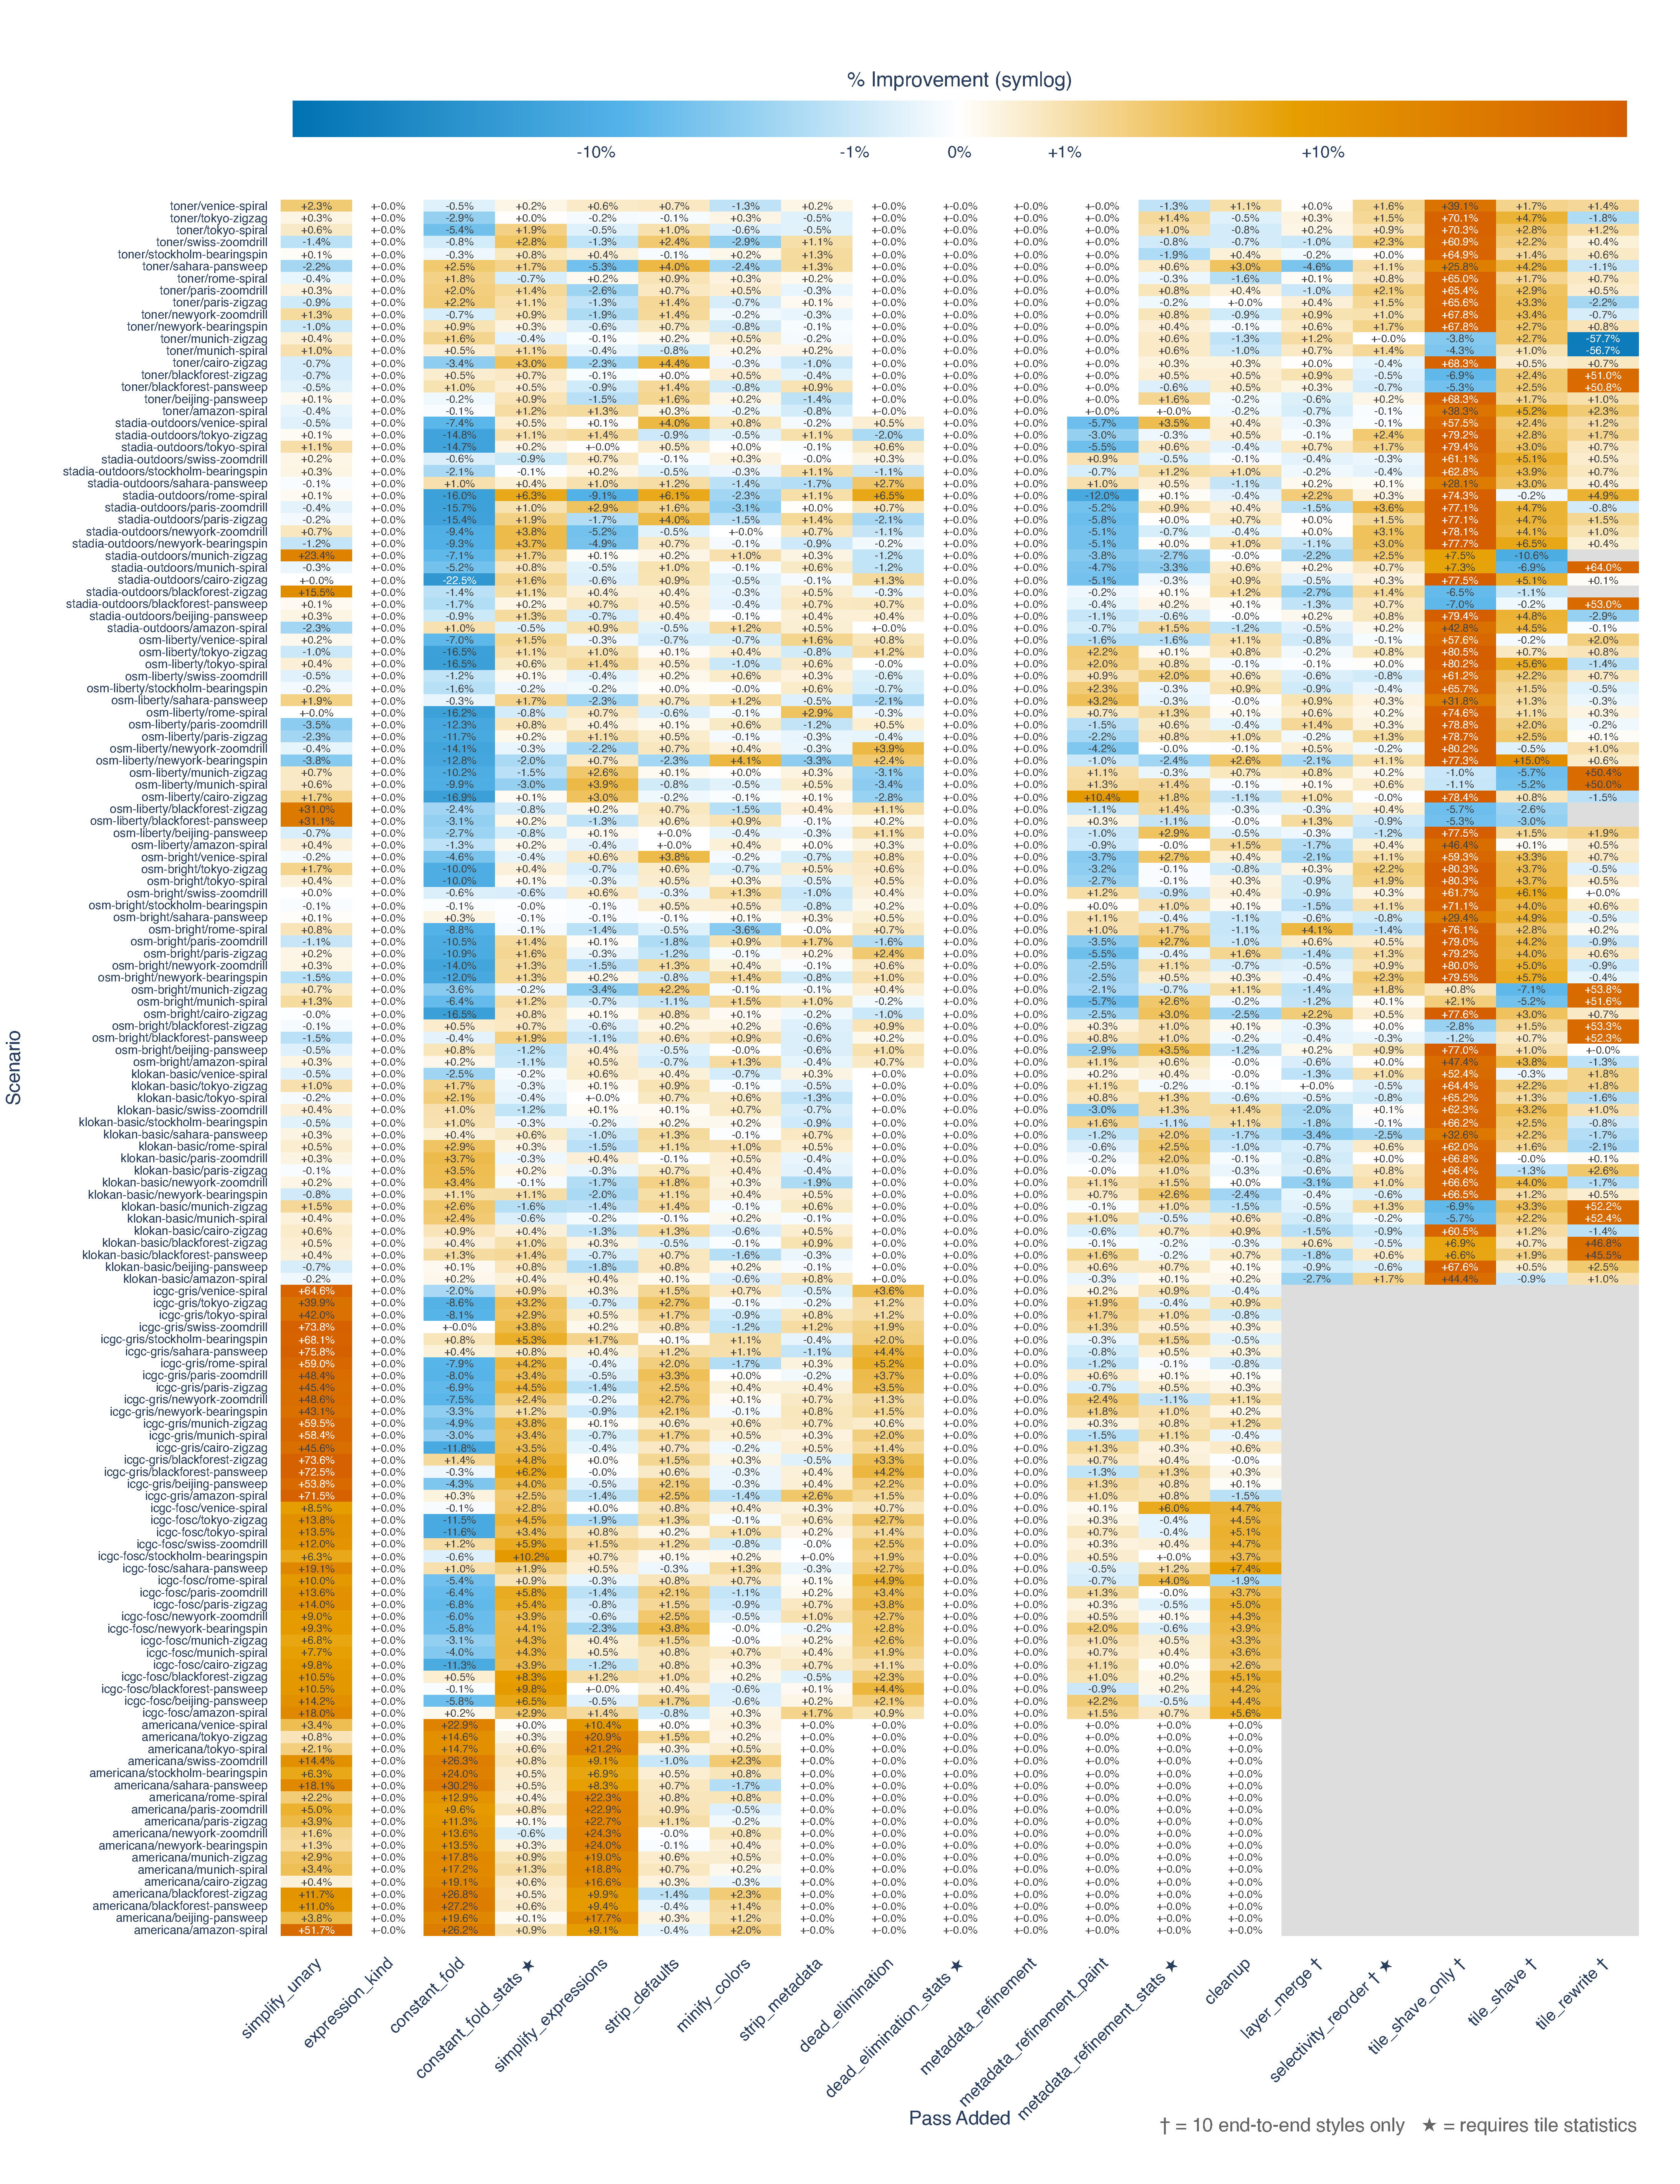
\includegraphics[height=0.9\textheight]{figures/heatmap_loadMs.pdf}
	\caption{
Heatmap of load time across scenarios (rows) and ablation steps (columns), where darker cells indicate greater improvement relative to baseline.
Urban, tile-dense scenarios (New York, Tokyo, Paris) show the largest absolute improvements.
Structural passes produce concentrated gains where dead elimination or layer merging applies.}
	\label{fig:heatmap_loadMs}
\end{figure}

\begin{figure}[htbp]
	\centering
	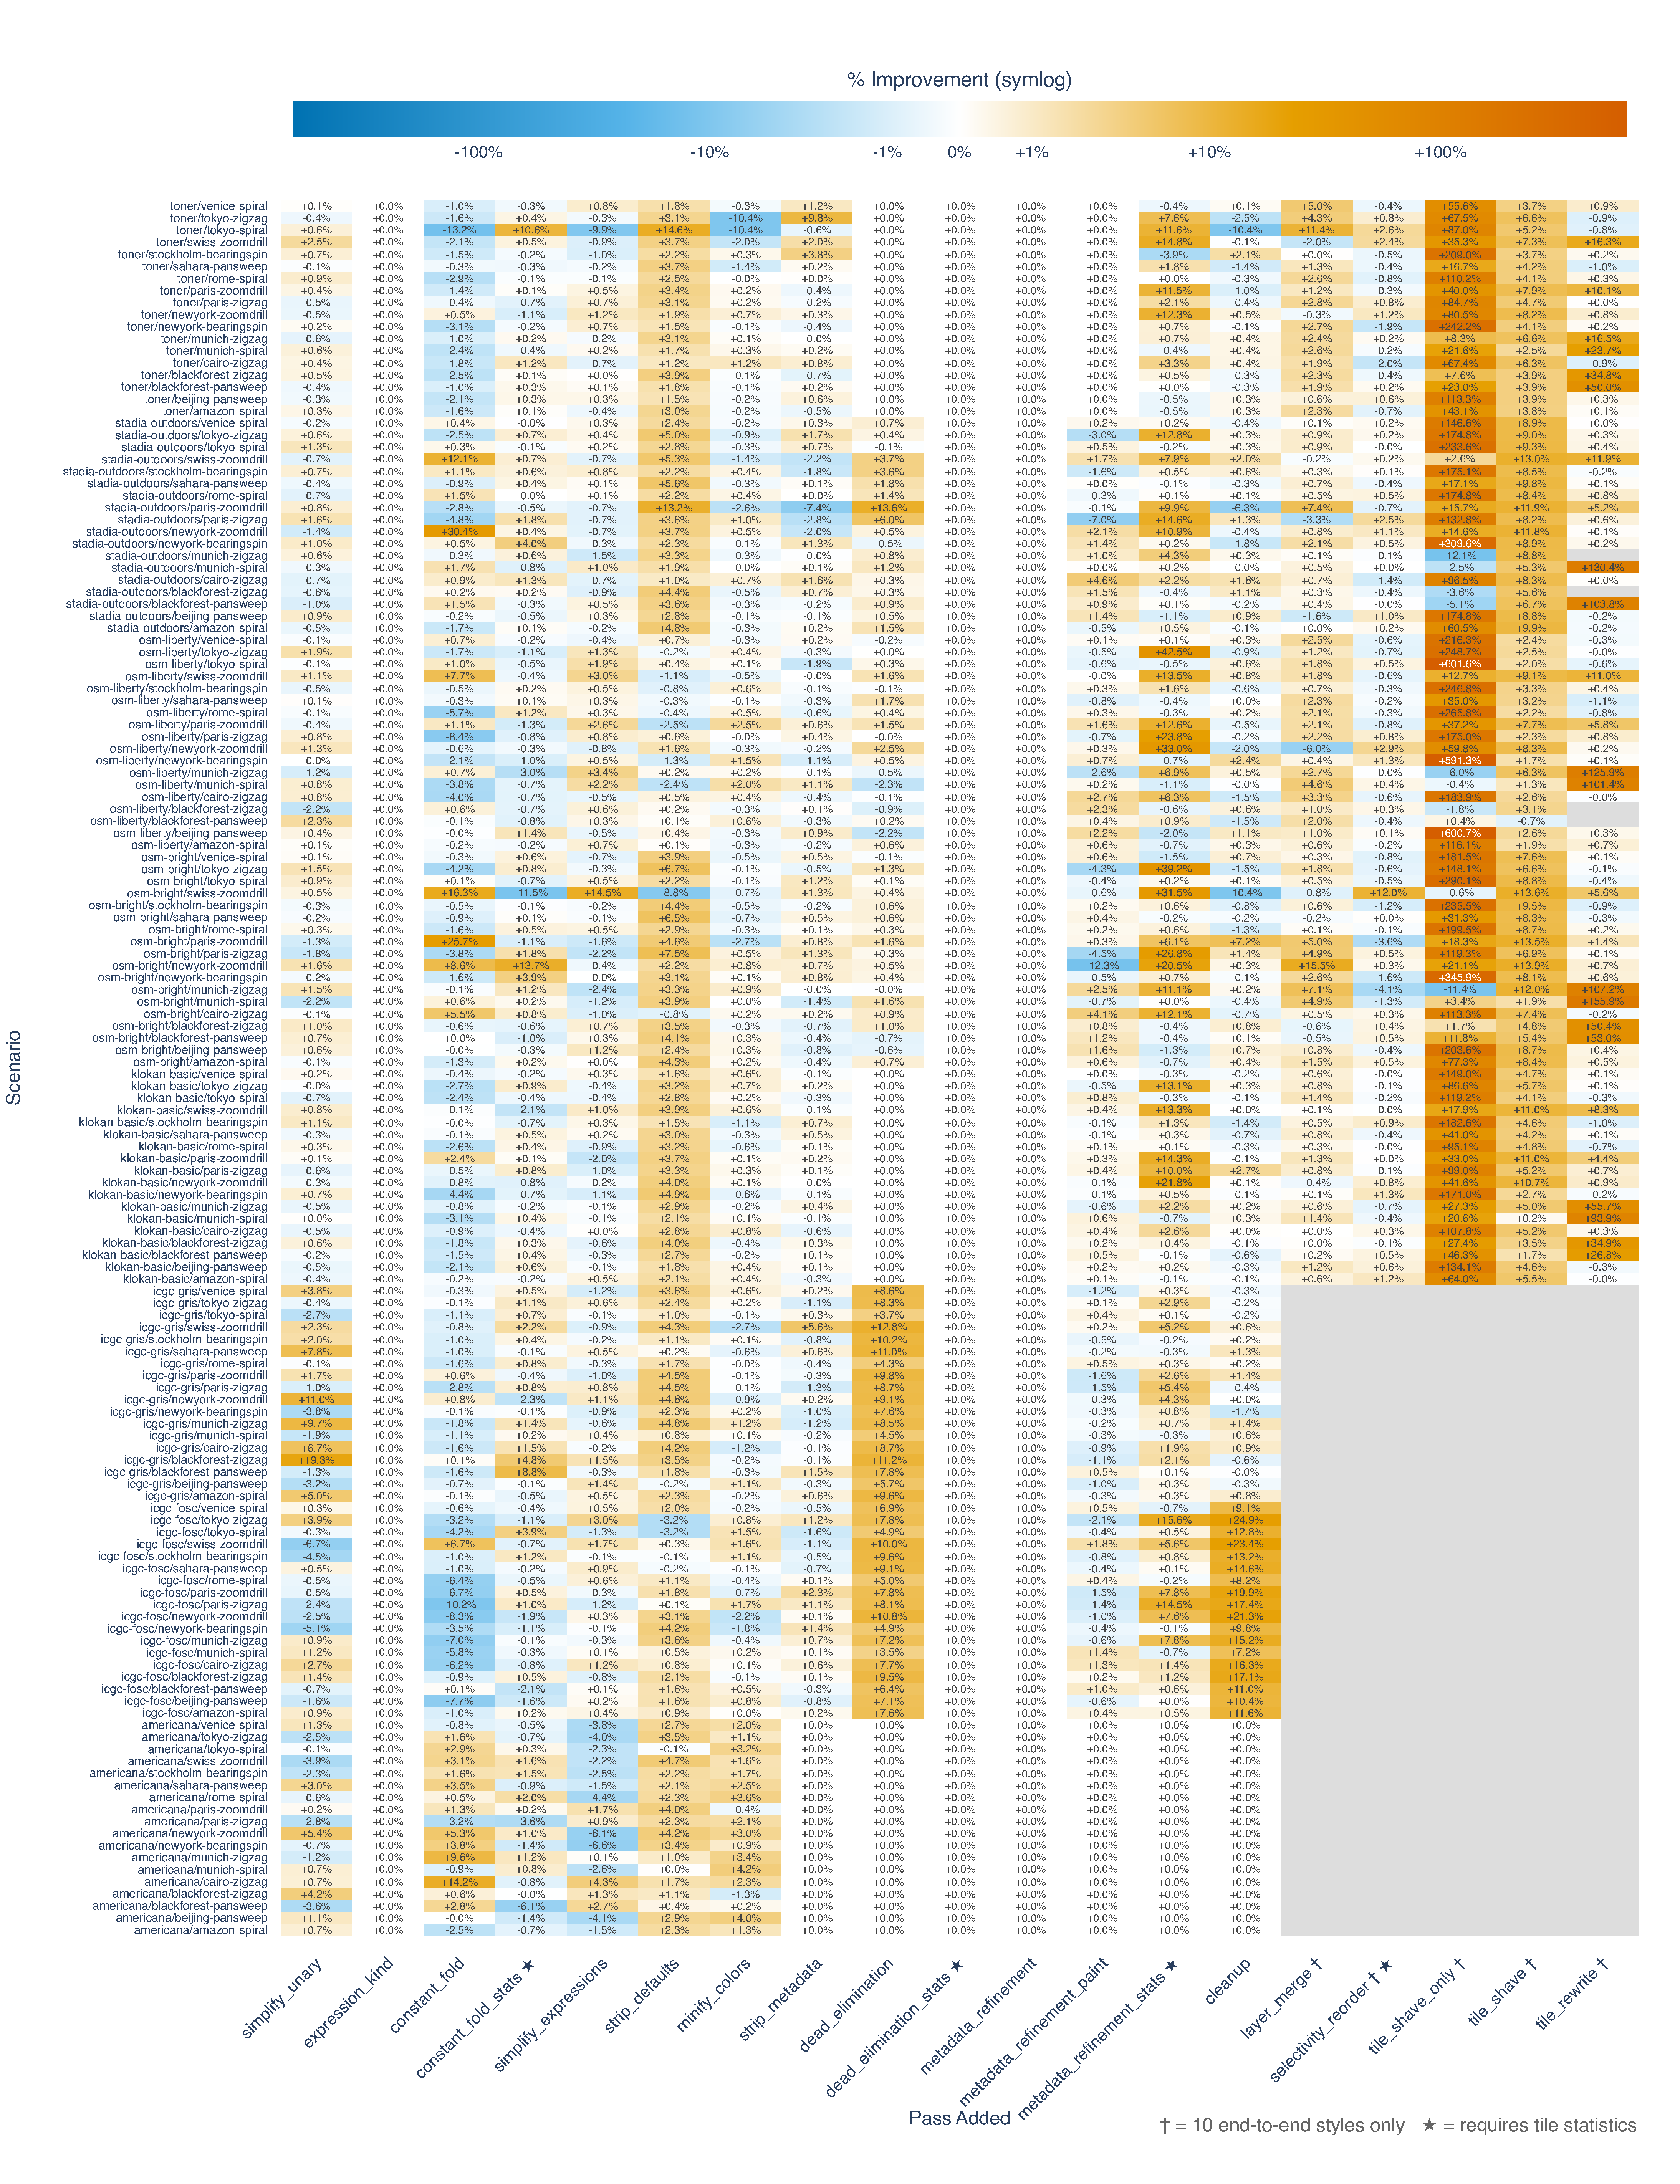
\includegraphics[height=0.9\textheight]{figures/heatmap_fps.pdf}
	\caption{
Heatmap of \ac{FPS} across scenarios (rows) and ablation steps (columns).
Compared to \cref{fig:heatmap_loadMs}, the \ac{FPS} gains are distributed more uniformly across scenarios, since sustained frame rate is driven by per-feature evaluation cost rather than by tile-fetch latency once tiles are resident.}
	\label{fig:heatmap_fps}
\end{figure}

\begin{figure}[tbph]
	\centering
	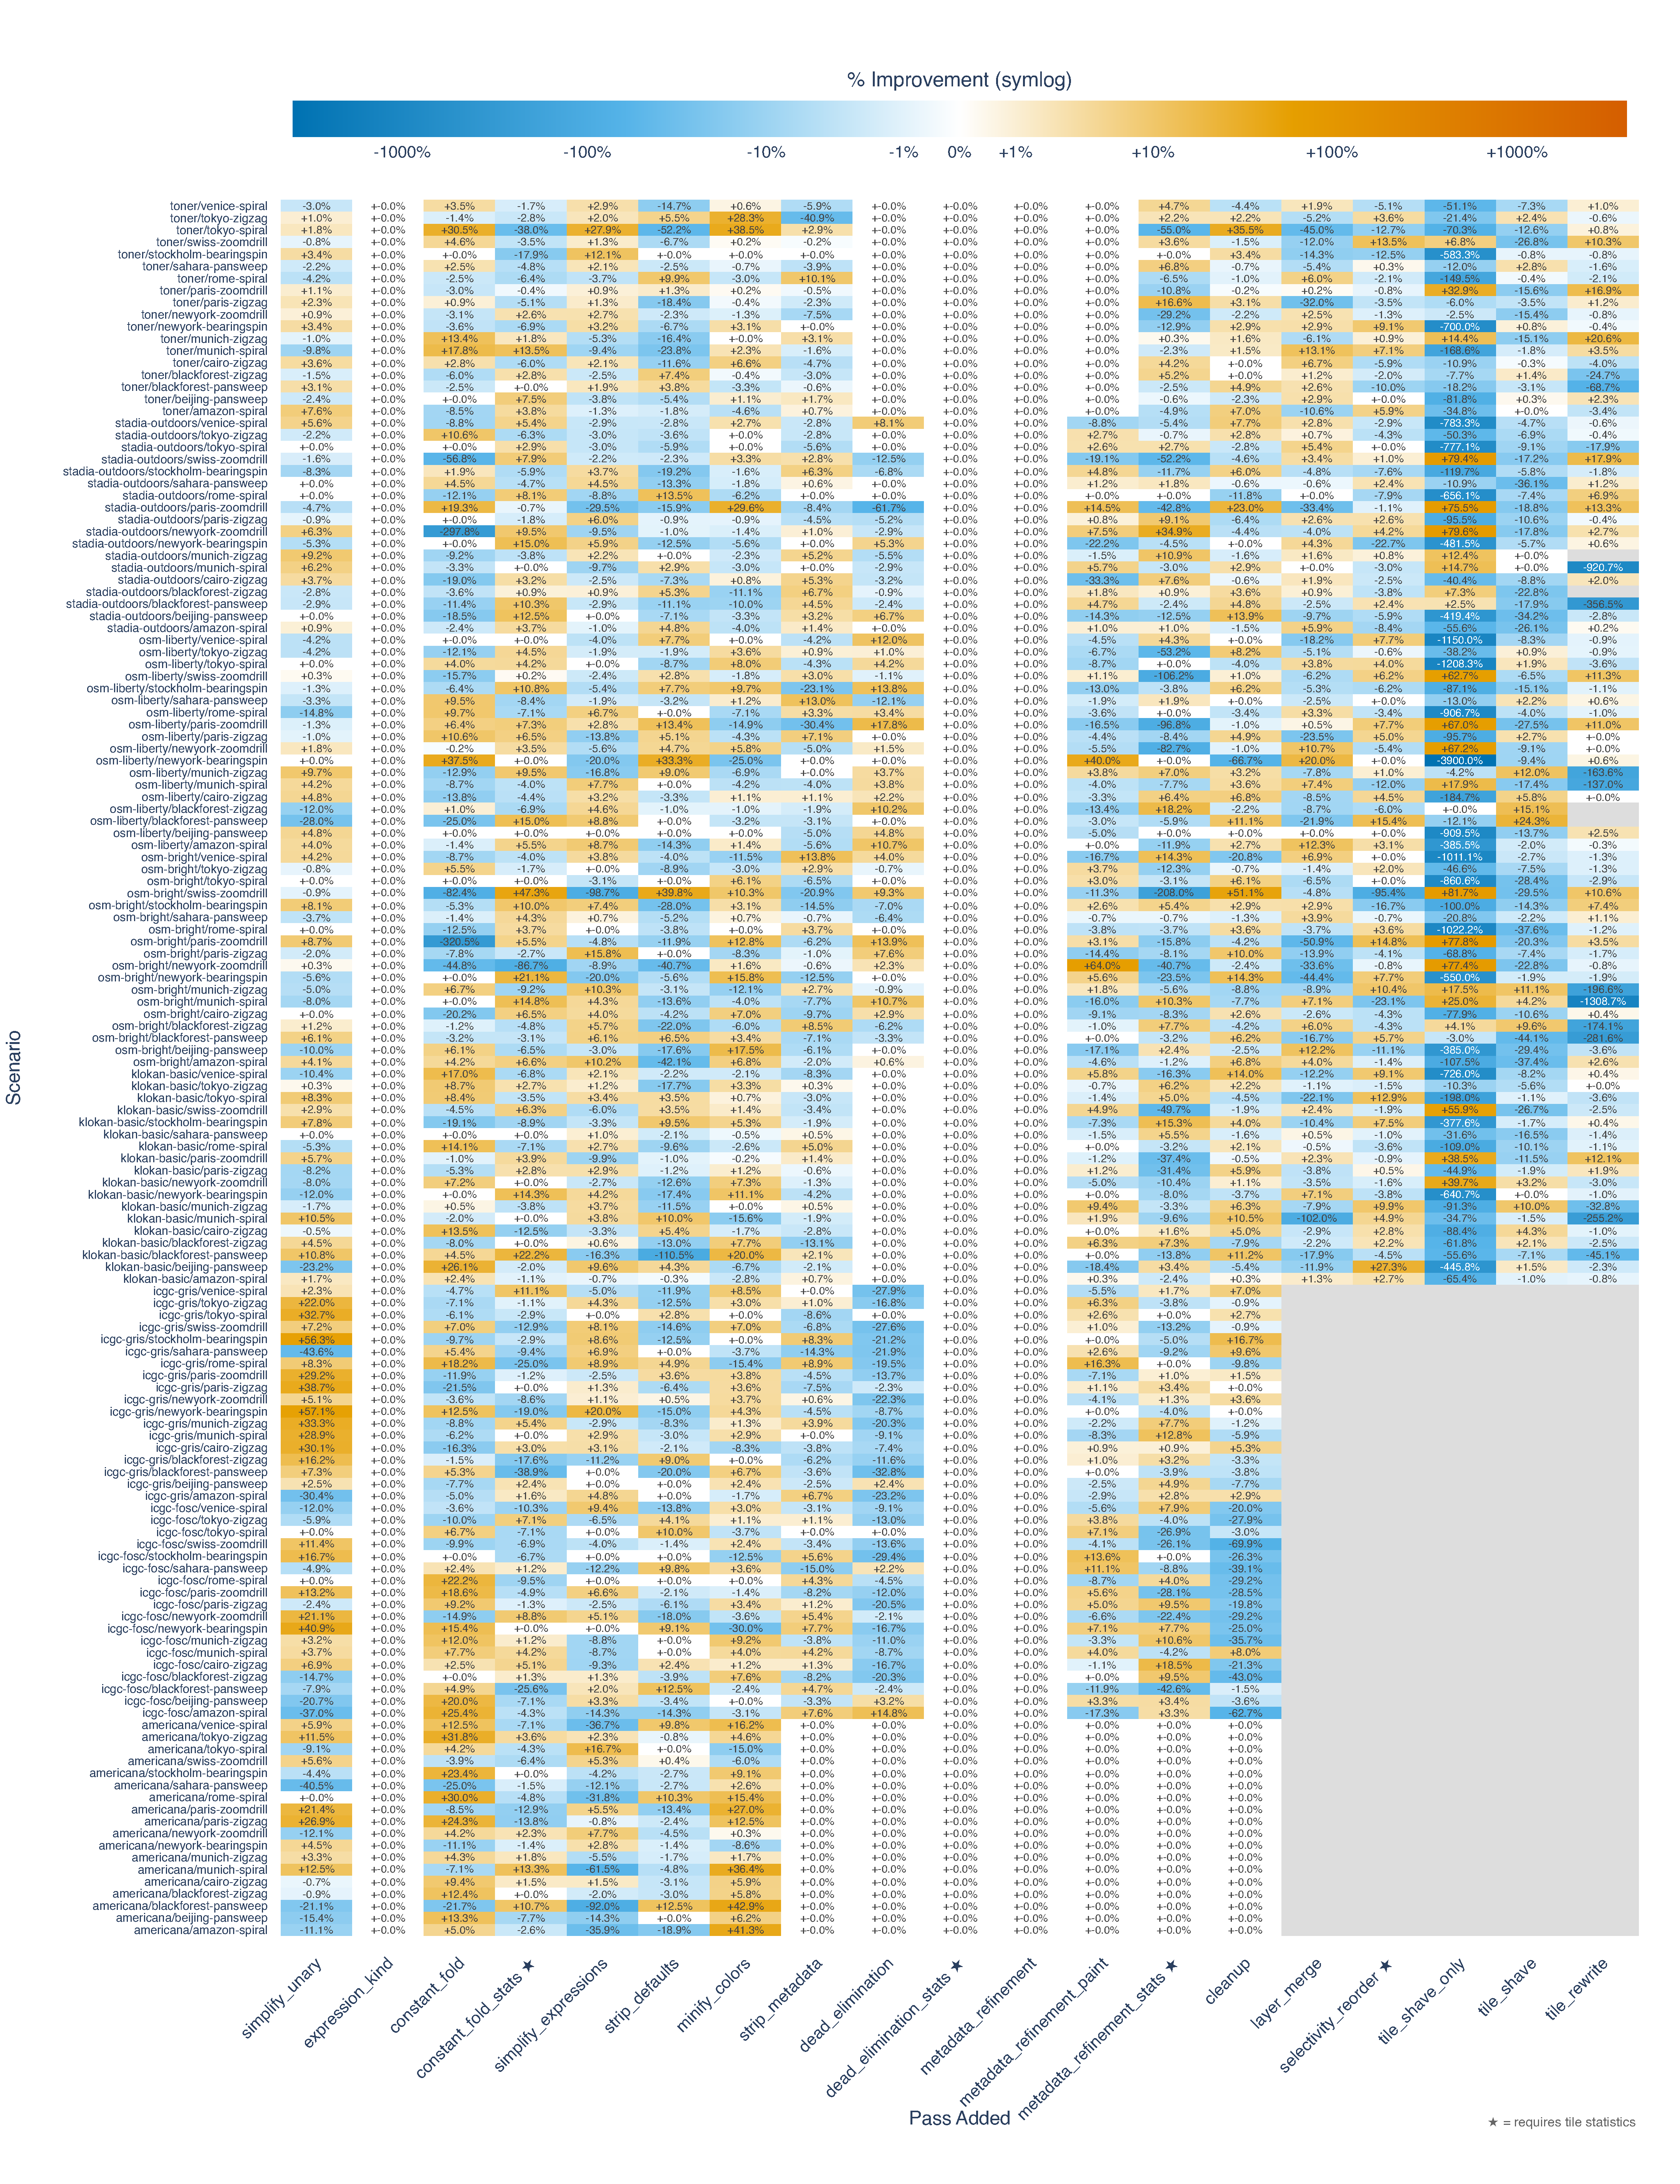
\includegraphics[height=0.9\textheight]{figures/heatmap_jankCount}
	\caption{
Heatmap of jank-frame counts (frame times substantially slower than their neighbours) across scenarios and ablation steps.
Counts increase across the ablation because sustained frame rates above 2000\,\ac{FPS} expose small \ac{GC}-pauses as proportionally large outliers.
Real consumer hardware caps well below this rate, so the same pauses would not cross the jank threshold there.}
	\label{fig:heatmapjankcount}
\end{figure}

\cref{fig:time_breakdown} decomposes load time across ablation steps.
The style-parse component shrinks monotonically with each expression pass, while first-tile and remaining-load are unchanged by style-only steps and drop only once tile shaving fires at steps~17-19.

\cref{fig:memory_ablation} tracks browser heap memory.
Style-level passes drift the resident JS heap from a baseline of \qty{86.0}{\mega\byte} to \qty{82.9}{\mega\byte} by step~15 (\qty{-3.6}{\percent}), with no single pass dominating.
Data-level passes drive the bulk of the reduction: tile shaving (step~17) alone drops the heap to \qty{63.7}{\mega\byte}, and the full pipeline reaches \qty{55.3}{\mega\byte} at step~19 (\qty{-35.7}{\percent} cumulative), reflecting that the major heap consumer is the in-memory tile payload rather than the parsed style.

\begin{figure}[htbp]
    \centering
    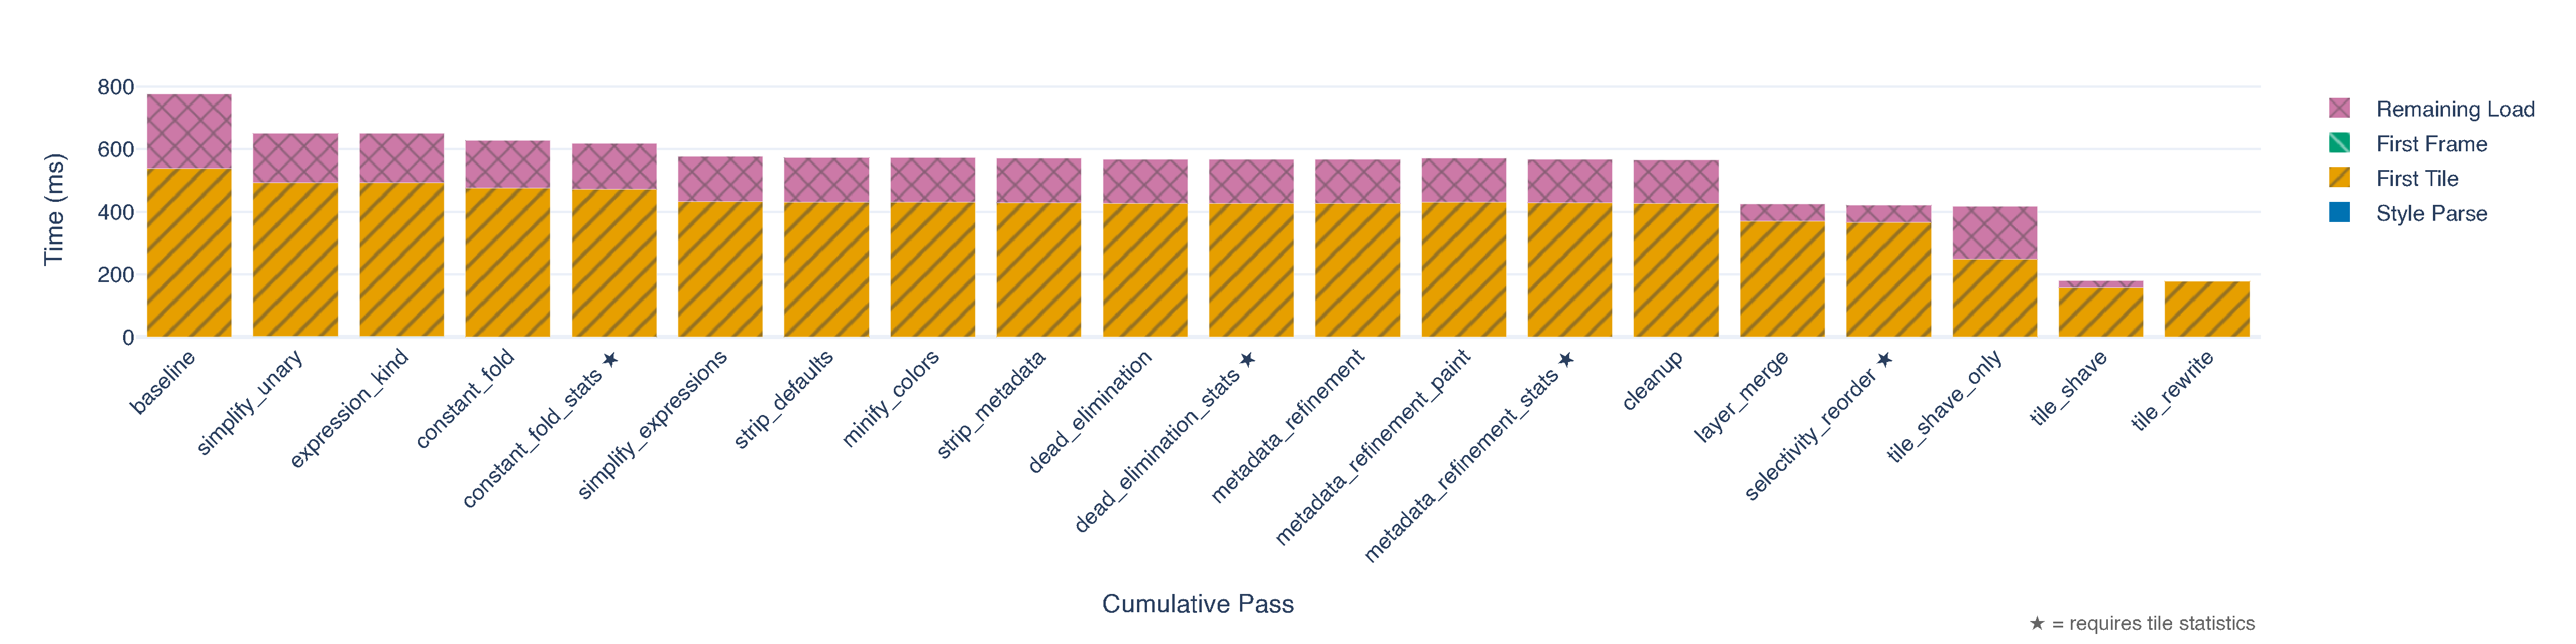
\includegraphics[width=\linewidth]{figures/time_breakdown.pdf}
    \caption{
Time breakdown across ablation steps: style parse, first tile, first frame, and remaining load time.
Style-parse time shrinks monotonically with each expression pass.
First-tile and remaining-load times are unchanged by style-only steps and decrease only when tile shaving is applied (steps~17-19).}
    \label{fig:time_breakdown}
\end{figure}

\begin{figure}[htbp]
    \centering
    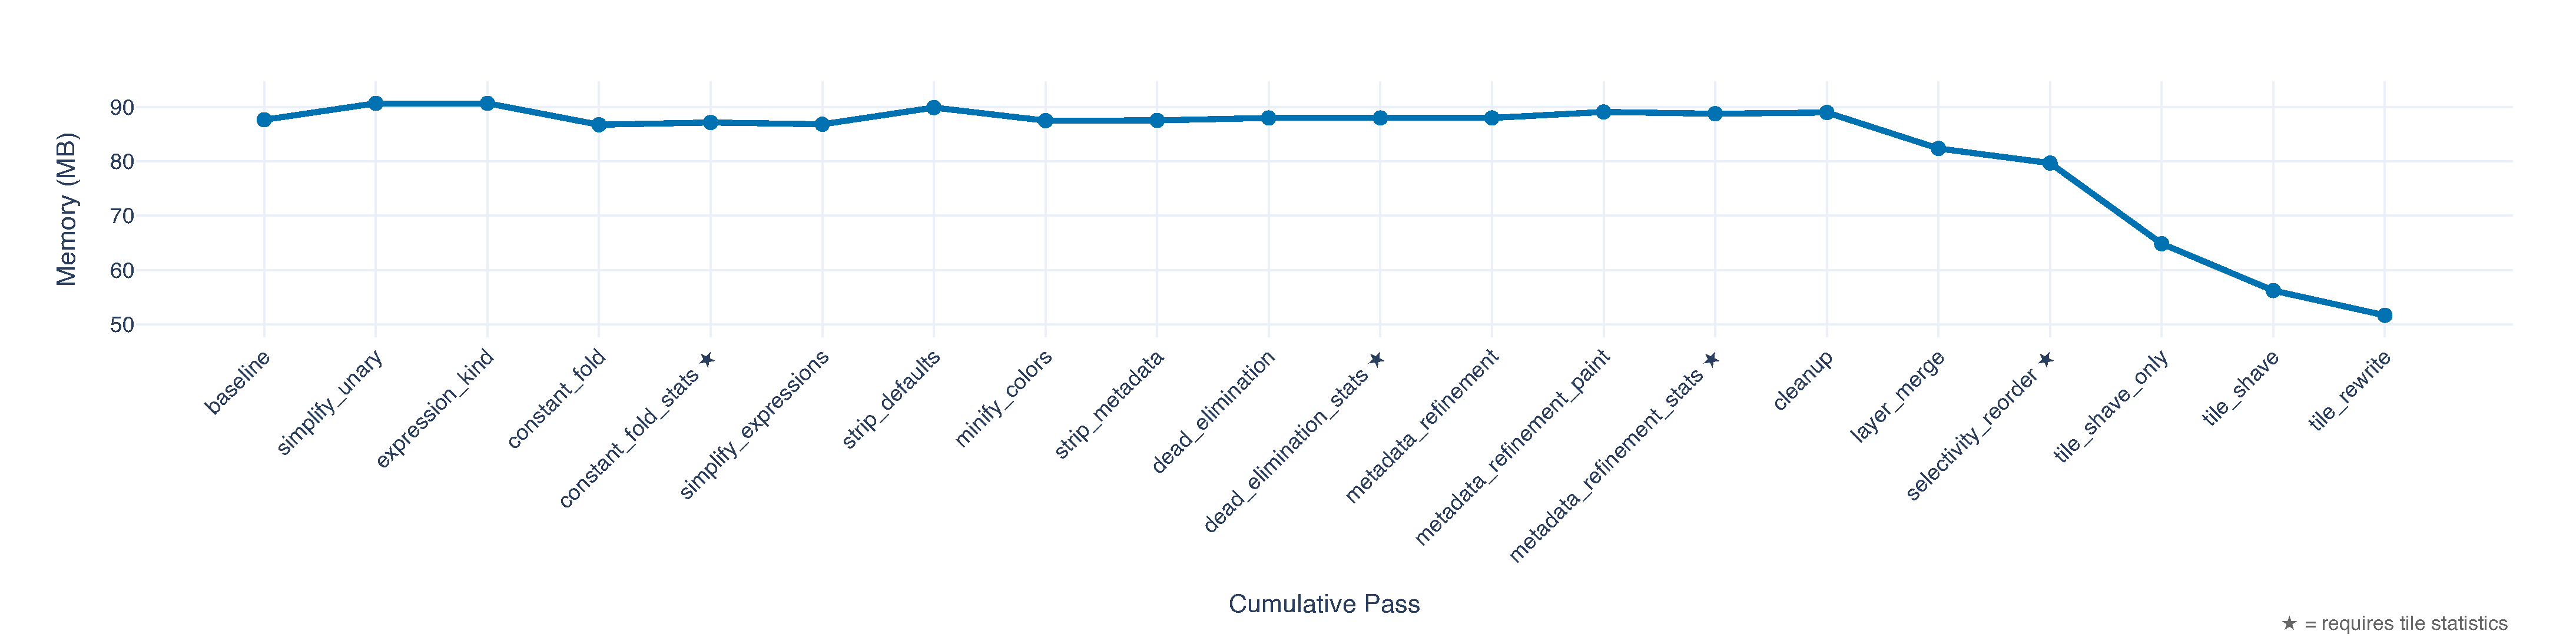
\includegraphics[width=\linewidth]{figures/memory_ablation.pdf}
    \caption{
Heap memory usage (mean \texttt{heapUsedMB} across all scenarios and benchmark styles) across ablation steps.
Style-level passes (steps 1-15) reduce the heap by \qty{3.1}{\mega\byte} (\qty{-3.6}{\percent}).
The bulk of the heap savings comes from data-level passes (steps 17-19) where the in-memory tile payload itself shrinks, yielding a cumulative reduction of \qty{-35.7}{\percent} from baseline to step~19.}
    \label{fig:memory_ablation}
\end{figure}

\begin{table}[htbp]
\centering\small
\csvreader[
  tabular=l r r r r r,
  table head={\toprule
    \textbf{Style} & \textbf{Baseline} & \textbf{Optimised} &
    \textbf{Reduction} & \textbf{$\Delta$ Load} & \textbf{$\Delta$ FPS} \\
     & \textbf{gzip (B)} & \textbf{gzip (B)} &
     \textbf{(\%)} & \textbf{(\%)} & \textbf{(\%)} \\
    \midrule},
  table foot=\bottomrule,
  head to column names,
  before line={\ifnum\midruleBefore=1\midrule\fi},
]{scripts/data/per_style_summary.csv}{}%
{\ifnum\isBold=1\textbf{\style}\else\style\fi &
 \num{\baseGzip} & \num{\optGzip} & \reduction &
 \fmtdelta{\deltaLoad} & \fmtdelta{\deltaFps}}%
\caption{
Per-style summary: baseline and optimized style size (gzip), size reduction, and change in load time and \ac{FPS} (medians across scenarios).
Styles below the rule include tile-level optimizations (steps~1-19), and those above include style-level optimizations only (steps~1-15).
Tile shaving produces the most visible drops in load time and \ac{FPS} improvements.}
\label{tab:per_style_summary}
\end{table}

\begin{table}[htbp]
\centering
\small
\csvreader[
  tabular=r l r r r r r,
  table head={\toprule
    \textbf{Step} & \textbf{Pass} & \textbf{$\Delta$ Raw} &
    \textbf{$\Delta$ Gzip} & \textbf{$\Delta$ Brotli} &
    \textbf{$\Delta$ Load} & \textbf{$\Delta$ Layers} \\
     & & \textbf{(\%)} & \textbf{(\%)} & \textbf{(\%)} & \textbf{(\%)} & \\
    \midrule},
  table foot={\midrule
    \multicolumn{7}{l}{\footnotesize $\dagger$ Steps~16-19:
    fiord and liberty only (benchmarked with tile statistics).} \\
    \bottomrule},
  head to column names,
]{scripts/data/marginal_contribution.csv}{}%
{\step & \pass\ifnum\dagger=1\textsuperscript{$\dagger$}\fi &
 \fmtdelta{\deltaRaw} & \fmtdelta{\deltaGzip} & \fmtdelta{\deltaBrotli} &
 \fmtdelta{\deltaLoad} & \fmtdeltaint{\deltaLayers}}%
\caption{
Marginal contribution of each ablation step to style size (raw, gzip, Brotli), load time, and layer count.
Values are percentage of baseline, medians across 12 styles and 18 scenarios.
Data-level tile shaving dominates transfer-size and load-time metrics.
Style-level passes contribute primarily to parse-time and style-size reductions and serve as enablers for the data-level pipeline.}
\label{tab:marginal_contribution}
\end{table}

\subsection{Marginal Contribution Analysis}\label{sub:combined_marginal}

Not all passes contribute equally, and the marginal contribution of each pass depends on the metric under consideration.

\paragraph{Rendering Time Metrics}
After tile shaving, we observe that expression-level constant folding and structural dead elimination tend to produce the largest marginal improvements in frame time and \ac{FPS}, as they reduce the number of expressions the renderer must evaluate per feature per frame and the number of layers it must process, respectively.
Layer merging produces a large marginal improvement in draw-call-heavy styles (many road layers, many boundary layers) but a smaller improvement in simple styles.

\paragraph{Transfer Size Metrics}
Passes that primarily reduce serialized style size (default stripping, metadata stripping, color minification) show smaller rendering improvements but contribute meaningfully to transfer size, particularly under compression (gzip, Brotli).
A smaller style reduces the time to first render because the \ac{JSON} must be fetched, decompressed, and parsed before the renderer can initialise.
Data-level tile shaving dominates the transfer-size metric, as tiles are fetched continuously during map interaction whereas the style is loaded only once.

\paragraph{Load Time Metrics}
Both style size (initial fetch and parse) and tile size (first tile fetch) influence load time.
Style-level passes improve style parse time.
Data-level passes improve first-tile time.
The relative contribution depends on the network bandwidth.
Under the \qty{10}{\Mbps} throttle, tile-fetch latency dominates.
Under the \qty{1.5}{\Mbps} throttle, style-fetch latency becomes significant for large styles.

\subsection{Preprocessing Cost}\label{sub:preprocessing_cost}

Research Goal~R3 asks how expensive the optimizations are in terms of preprocessing time.
The optimizations pipeline is an \emph{offline} stage: we optimize a style once and serve it many times, and re-encode tiles once per tileset build.
Preprocessing cost is therefore amortised over all subsequent tile deliveries and is not on the user's critical path, but it still matters for operational feasibility on large tilesets.

In this section we measure each of the four additive cost terms $C_\text{style}$, $C_\text{stats}$, $C_\text{adv}$, and $C_\text{enc}$ from the preprocessing cost model (\cref{eq:cost_model}, \cref{sub:preprocessing_cost_model}) on a real tileset, and confirm that the cost-control mechanisms formalised there keep the multi-strategy overhead well below the naive worst case.

\paragraph{Measured Stage Costs}
\Cref{tab:preprocessing_cost} reports wall-clock time for each stage of the preprocessing pipeline on the Germany OpenMapTiles tileset (\num{256156} tiles after pruning, zoom 0-14), which we measured on an AMD Ryzen~7 3700X (8 cores / 16 threads), \qty{46}{\gibi\byte} \ac{RAM}, NVMe SSD (median of three runs).
\emph{Style optimization} ($C_\text{style}$) and \emph{advisory computation} ($C_\text{adv}$) are negligible: Liberty's 111-layer style completes all passes in \qty{7.5}{\milli\second} and the advisory in \qty{1.1}{\milli\second}.
\emph{Tile-statistics collection} ($C_\text{stats}$) takes \qty{57.4}{\second} for a single-threaded scan of all \num{256588} source tiles.
\emph{Tile pruning and \ac{MVT} re-encoding} ($C_\text{enc}$, MVT) takes \qty{15.6}{\second} using Rayon\footnote{\url{https://github.com/rayon-rs/rayon}, last accessed 2026-05-23} parallelism.
\emph{\ac{MLT} encoding with sort-strategy competition} ($C_\text{enc}$, \ac{MLT} auto) is the dominant term: \qty{5}{\minute}\,\qty{42}{\second} single-threaded, or \qty{47}{\second} with 16 threads.
Without the competition ($C_\text{enc}$, \ac{MLT} none), single-threaded encoding takes \qty{2}{\minute}\,\qty{55}{\second}.
We therefore measure the overhead ratio of the full competition at $342 / 175 = 1.95\times$ in \ac{CPU} time, substantially lower than the analytical 3-5$\times$ estimate, because the cost-control mechanisms formalised in \cref{sub:preprocessing_cost_model} eliminate most redundant work.

\begin{table}[htbp]
\centering\small
\begin{tabular}{l l r}
\textbf{Stage} & \textbf{Description} & \textbf{Wall-clock} \\
\midrule
$C_\text{style}$ & Style optimization (all passes, Liberty) & \qty{7.5}{\milli\second} \\
$C_\text{stats}$ & Tile statistics (\num{256588} tiles, 1 thread) & \qty{57.4}{\second} \\
$C_\text{adv}$ & Advisory computation & \qty{1.1}{\milli\second} \\
$C_\text{enc}$ (\ac{MVT} prune) & Tile pruning + \ac{MVT} re-encode (16 threads) & \qty{15.6}{\second} \\
$C_\text{enc}$ (\ac{MLT} none, 1T) & \ac{MLT} encoding, single strategy, 1 thread & \qty{175}{\second} \\
$C_\text{enc}$ (\ac{MLT} auto, 1T) & \ac{MLT} encoding, full competition, 1 thread & \qty{342}{\second} \\
$C_\text{enc}$ (\ac{MLT} auto, 16T) & \ac{MLT} encoding, full competition, 16 threads & \qty{46.7}{\second} \\
\midrule
Overhead factor & auto\,/ \,none (single-threaded CPU time) & $1.95\times$ \\
\end{tabular}
\caption{
Preprocessing wall-clock time per pipeline stage on the Germany OpenMapTiles tileset (zoom 0-14, \num{256156} tiles after pruning) when run on \cref{tab:bench_hardware}.
Median of 3~runs.
Style optimization ($C_\text{style}$, \qty{7.5}{\milli\second}) and advisory computation ($C_\text{adv}$, \qty{1.1}{\milli\second}) are negligible; \ac{MLT} encoding with full sort-strategy competition dominates at \qty{342}{\second} single-threaded (\qty{46.7}{\second} with 16 threads), with an overhead factor of $1.95\times$ vs.\ a fixed-plan encoder.}
\label{tab:preprocessing_cost}
\end{table}

\paragraph{Amortisation and Headline Numbers}
Taken together, the cost-control mechanisms formalised in \cref{sub:preprocessing_cost_model} (bounding-box pruning, data profiling, warm-start caching, scratch-buffer recycling, and the \ac{RAII} alternatives guard) reduce the measured overhead of the full sort-strategy competition to $1.95\times$ compared to a fixed-plan (single-strategy) encoder (\cref{tab:preprocessing_cost}), well below the naive $4\times$ expectation from four candidate sort orders.
We empirically confirm that the trial-and-retain loop costs $k$ encode passes plus $\mathcal{O}(1)$ bookkeeping rather than $k$ encode passes plus $k$ full buffer clones.
We pay this cost once per tileset build and amortise it over every subsequent tile request.
The total single-threaded pipeline time (statistics collection through \ac{MLT} encoding with full competition) is under \qty{7}{\minute} on the Germany tileset.
With 16-thread parallelism the end-to-end wall-clock time drops to approximately \qty{2}{\minute}, perfectly acceptable for an offline build stage.
The effect of this on client side performance is not as big as it could currently be, because internally we transform data to \acsp{MVT} instead of a more efficient in-memory-structure.

\subsection{Complexity Metrics}\label{sub:combined_complexity}

The four complexity metrics we track across ablation steps (\cref{sub:metrics}) give a structural explanation for the observed rendering improvements.
Expression passes (constant folding, simplification) drive the largest reductions in \ac{AST} node count.
Boolean flattening and De~Morgan rewrites drive the maximum-depth reductions.
Dead elimination and layer merging drive the layer-count reductions.
Metadata refinement (by consuming zoom predicates) together with dead elimination drive the filter-count reductions.
Where the same step appears across two complexity axes, we describe the connection to the corresponding rendering metric in \cref{sub:combined_marginal}.

\subsection{Discussion}\label{sub:combined_discussion}

Composed end-to-end across the ten deep-corpus styles, the full pipeline cuts per-style median load time by \qty{71}{\percent} and lifts \ac{FPS} by \qty{152}{\percent}.
The three optimization channels (expression, structural, data) compose additively because they target non-overlapping costs (simplification cannot shrink tiles, shaving cannot prune expressions).
The following paragraphs decompose which channel each family acts on, separate the load-time levers from the frame-rate levers, and close with the measurement-noise caveats that bound these numbers.

\paragraph{Three Plausible Improvement Channels}
The full pipeline ablation points to three plausible channels, which we infer from proxy metrics (\ac{AST} node count, layer count, tile size) and the time breakdown (\cref{fig:time_breakdown}) since no renderer instrumentation separates them directly.
The expression passes (\cref{sub:expression_optimizations}) plausibly reduce per-feature evaluation cost.
Fewer \ac{AST} nodes mean fewer interpreter steps per feature per frame.
Dead elimination and layer merging (\cref{sub:structural_optimizations}) operate one level up, cutting draw calls, \ac{GPU} state changes, and per-layer filter evaluations.
Tile shaving and re-encoding (\cref{sub:data_optimizations}) act on transfer and decode cost so load time and time-to-first-tile drop, with a secondary effect on average frame time via lower \ac{GC}-spend.

\paragraph{Load Time vs.\ Frame Rate}
Expression and structural passes improve both load time and frame rate, because a simpler style is both faster to parse and faster to render.
Data-level passes primarily improve load time (smaller tiles arrive faster) and have a smaller effect on sustained frame rate, since once tiles are decoded and resident in the \ac{GPU} the per-frame cost is dominated by expression evaluation and draw-call overhead rather than data size.
The exception is tile shaving at overview zoom levels, where removing entire source-layers reduces the number of features the renderer must process per frame.

\paragraph{What Varies, and Why}
The cumulative ablation shows diminishing marginal returns:
early passes (constant folding, dead elimination) capture the largest improvements because they address the most common sources of waste, while later passes (color minification, metadata stripping) address less frequent patterns and contribute correspondingly less.
The non-cumulative isolated-impact analysis confirms that each pass has a non-trivial standalone contribution, even when its cumulative-sequence contribution looks small.
The marginal number is sensitive to which passes precede it, but the standalone number is not.

Variation across styles is similarly structured:
styles with many narrowly-filtered layers (e.g.\ detailed road styles) benefit most from layer merging, styles with broad filters from stats-driven dead elimination, and styles with large expression trees from constant folding.
No single pass dominates across all styles, which is the empirical justification for the multi-pass design.

\paragraph{Measurement Noise}
The 15-run median smooths out most measurement noise, but tail metrics (p99 frame time, jank count) carry higher variance than central-tendency metrics; \ac{GPU} thermals, browser garbage collection, and OS scheduling all contribute.
We partly self-inflict this: using real \ac{GPU} hardware (ANGLE/Vulkan) rather than a software rasteriser captures realistic rendering costs (\ac{GPU} buffer management, shader compilation) at the expense of slightly higher noise compared to deterministic software rendering.


\section{Visual Correctness Validation}\label{sec:visual_correctness}

We verified visual losslessness (\cref{eq:visual_equivalence}, with the per-pass soundness arguments collected in \cref{sec:building_optimizations}) with pixelmatch\footnote{\url{https://github.com/mapbox/pixelmatch}, last accessed 2026-05-23} across all 15 benchmark styles at zoom levels~0-14, across all 18 scenarios from \cref{sub:scenarios}, in both axis-aligned and pitched views, at \texttt{pixelRatio}~1 and using MapLibre GL~JS's Node-side software rasteriser.
Across every comparison, the fraction of differing pixels stayed below pixelmatch's per-test tolerance (default \texttt{allowed}~$=0.00025$ at the YIQ-perceptual \texttt{threshold}~$=0.1285$), confirming that every optimizations pass preserves visual identity on the software rasteriser within the perceptual-difference budget used by the upstream MapLibre render harness.

\section{Threats to Validity}\label{sec:threats}

In this section we discuss potential threats to the validity of the experimental findings.

\paragraph{Internal Validity}
We conducted all rendering benchmarks on a single hardware configuration (\ac{GPU} model, \ac{CPU}, memory) running a specific browser version with ANGLE/Vulkan as the graphics backend.
The full host, driver, toolchain, and dependency dump is in \cref{app:bench_env}.
Performance characteristics may differ on other hardware or with different graphics backends (e.g., native OpenGL, DirectX, Metal).
We chose the 15-run median to reduce measurement noise, but rare performance events (e.g., \ac{GPU} thermal throttling, garbage collection pauses) may not be fully captured.
The caching proxy eliminates network variability but also prevents observation of real-world caching effects and \ac{CDN} behavior.

\paragraph{External Validity}
We limit the evaluation to MapLibre GL~JS.
Results may not transfer directly to other renderers such as Mapbox GL~JS, deck.gl, or native MapLibre implementations.
The tile data uses only OpenMapTiles and BasemapDE schemas.
Other schemas with different property distributions or geometry characteristics may yield different optimizations gains.
The 15 benchmark styles, while diverse, may not represent all style authoring patterns encountered in production deployments.

\paragraph{End-to-End Data-Level Coverage}
We benchmark the full rendering pipeline (style optimizations through tile shaving to \ac{MLT} re-encoding) end-to-end on 10 of the 15 deep-corpus styles (bright, dark-matter, fiord, klokan-basic, liberty, osm-bright, osm-liberty, positron, stadia-outdoors, toner).
ICGC Fosc and ICGC Gris were excluded because the legacy \mlprop{\texttt{text-field}} handling described in \cref{sub:deep_corpus} renders incorrectly under MapLibre's silent migration.
The BasemapDE pair was excluded because its tile source is not \ac{OMT}-compatible and we could not provision matching shaved tiles.
For the remaining \ac{OMT}-compatible deep-corpus styles we verified the tile-shaving step alone (advisory generation and \ac{MVT} pruning, without rendering) on the same Germany tileset (\cref{fig:tile_shave_per_style}), confirming that shaving effectiveness generalizes across styles with reductions of \qtyrange{19.8}{46.3}{\percent}.
The remaining limitation is that tile statistics at a sample rate of~1.0 require access to the underlying tile data, which is available only for \ac{OSM}-based tilesets accessed via a local \texttt{.mbtiles} file.
The style-only results (Experiments~1-2) cover all 15 styles and are not affected by this limitation.

\paragraph{Construct Validity}
We simulate network conditions via a fixed bandwidth throttle (\cref{sub:tile_data}) rather than measuring under real \ac{CDN} latency profiles.
We designed the synthetic camera animations of \cref{sub:scenarios} (zigzag, spiral, zoomdrill, pansweep, bearingspin) to exercise diverse rendering workloads, but they may not capture typical user interaction patterns such as search-and-zoom workflows.

\paragraph{Statistical Validity}
The tile statistics (\cref{sub:tile_statistics}) count feature \emph{occurrences} across tiles, not unique geographic entities: a highway spanning 50 tiles is counted 50 times.
This inflates total feature counts and distorts absolute selectivity estimates, though relative selectivity ordering (which is all the reordering heuristic of \cref{sec:selectivity_reordering} consumes) is less affected.
We made this choice deliberatiley because the underlying features are not a concearn for the renderer on most layers (exception being symbol placement which is map-global instead of tile-local).

The selectivity estimation model assumes independence between filter predicates (\cref{eq:selectivity_compound}), which may not hold for correlated properties.
Map-style filters in practice do exhibit correlations (e.g.\ \mlval{\texttt{class}} and \mlval{\texttt{subclass}} in OpenMapTiles), so we treat the estimator as a first-order approximation rather than a calibrated model, and we understand selectivity-based reordering as a heuristic that produces a locally-good ordering rather than a provably-optimal one.

The 15-run median provides robustness against outliers but does not quantify sampling uncertainty on its own.
We computed bootstrap \qty{95}{\percent} confidence intervals~\cite{efronIntroductionBootstrap1998} (10\,000 resamples, percentile method) over the per-(style, variant) measurement pools for \texttt{loadMs} and \texttt{fps}.
Error bars in the waterfall (\cref{fig:waterfall_loadMs}), and rendering-metrics (\cref{fig:rendering_metrics_mlt}) figures represent these bootstrap \qty{95}{\percent} CIs.
Wilcoxon signed-rank tests (or Mann-Whitney~U where sample sizes differ) confirm that the full-pipeline load-time reductions are highly significant for both end-to-end styles (Fiord: \qty{370.9}{\milli\second}$\to$\qty{120.5}{\milli\second}, $p < 10^{-45}$, $n = 270$; Liberty: \qty{466.5}{\milli\second}$\to$\qty{133.7}{\milli\second}, $p < 10^{-74}$, $n = 254$).
Fiord's pool covers all 18 scenarios $\times$ 15 runs.
Liberty's full-pipeline pool covers 17 of 18 scenarios, with one scenario absent from the pipeline output and one scenario contributing 14 of 15 runs.
Because the 18 scenarios share hardware, tile data, and styles, they are not fully independent observations.
The effective sample size is smaller than $n = 270$, and we interpret the reported $p$-values as descriptive evidence of large effect sizes rather than as strict inferential tests.

Style-only effects on load time are smaller and, for individual styles, not consistently distinguishable from measurement noise.

The cumulative ablation design (\cref{sub:ablation}) means that the reported marginal contribution of each pass depends on the ordering of preceding passes.
A leave-one-out or fractional-factorial design would isolate each pass's standalone contribution more cleanly but we did not run it for cost reasons.

Tail metrics (p99 frame time, jank count) are particularly sensitive to sample size: with $n=15$ runs, the tail carries only a handful of informative samples per cell, and the reported numbers should be read as directional rather than conclusive.
The full-pipeline ablation performs thousands of pairwise comparisons across metrics, styles, scenarios, and ablation steps.
We apply no multiple-comparisons correction (Bonferroni, Benjamini-Hochberg), so individual per-cell \enquote{significant} differences should not be read as hypothesis tests, only as descriptive summaries.

\begin{chaptersummary}
Each pass family behaves differently in isolation.
Expression passes barely move load time on their own but enable the downstream passes.
The structural family's gains come almost entirely from dead-layer elimination and layer merging.
On the data side, \textbf{tile shaving dominates} with a \qty{-71.5}{\percent} \textbf{median load reduction}, while the \ac{MLT} encoder's per-stream strategy competition (not the format itself) delivers a further \qty{28}{\percent} tile-volume cut over the Java reference (\qty{12}{\percent} over gzip-compressed \ac{MVT}).
Composed end-to-end across the ten deep-corpus styles benchmarked with tile data, the full pipeline reduces load time by \qtyrange{63}{74}{\percent} (per-style median \qty{71}{\percent}) and improves \ac{FPS} by \qtyrange{100}{200}{\percent} (per-style median \qty{152}{\percent}), but the cross-family interaction is \textbf{additive rather than synergistic}.
The pooled Fiord+Liberty aggregate used in the \ac{MLT} discussion (\qty{+176}{\percent}) is a different aggregation of the same data restricted to the two end-to-end styles, not a conflicting headline.
The static passes generalize: a \textbf{median \qty{31.4}{\percent} raw style reduction across 13 unseen styles}, with none regressed.

The following chapter consolidates these findings into architectural claims, answers the research questions of \cref{sec:research_goals}, and identifies the directions left open.
\end{chaptersummary}

\chapter{Conclusion}\label{ch:conclusion}

In the preceding chapter we evaluated each optimization level in isolation and then measured their combined effect, revealing that tile shaving and columnar re-encoding dominate the load-time improvements while style-level passes provide modest, additive contributions.
This chapter consolidates those findings into architectural claims and answers the research questions posed in \cref{sec:research_goals}.

\section{Summary of Contributions}

This thesis makes four main contributions, mirroring the structure of \cref{sec:contributions}.

\begin{enumerate}[label=\textbf{C\arabic*}]
    \item The \textbf{formalization of joint style and tile co-optimization} as a transformation $\mathcal{O}: \mathcal{S} \times \mathcal{T} \to \mathcal{S} \times \mathcal{T}$ under visual equivalence and strict idempotency (\cref{sec:problem_statement}).
    The constraint pair held empirically.
    Our round-trip proptest and libFuzzer harness reported no soundness regressions across the corpus (\cref{par:encoder_validation}).

    \item The \textbf{three-level co-optimization strategy} of \cref{sub:pipeline}.
    The three levels turn out to be complementary rather than redundant (\cref{sub:combined_marginal}).
    Constant folding and dead elimination together account for the largest per-pass rendering gains.
    Style-driven tile shaving (\cref{sub:tile_shaving}) is the dominant contributor to load-time and transfer-size improvements.
    Adaptive multi-strategy encoding in our \ac{MLT} encoder (\cref{sub:data_optimizations}) reduces tile volume by \qty{28}{\percent} over the fixed-plan reference baseline.
    The advantage persists under every wire compressor tested (\cref{tab:mvt_mlt_comparison}).

    \item The \textbf{end-to-end implementation}, whose preprocessing cost we characterize on the Germany OpenMapTiles tileset (\cref{tab:preprocessing_cost}).
    The full single-threaded pipeline completes in under \qty{7}{\minute}.
    With 16-thread parallelism the wall-clock time drops to approximately \qty{2}{\minute}, paid once per tileset build and amortised over every subsequent tile request.
    The multi-strategy encoder competition increases single-threaded re-encoding cost by a factor of $1.95\times$ over a fixed-plan encoder.
    This is well below the naïve $4\times$ expectation, thanks to bounding-box pruning, data profiling, and warm-start caching.

    \item The \textbf{empirical evaluation} (\cref{ch:experiments}), conducted across 15 styles, 18 scenarios, and 19 cumulative ablation steps.
    The full pipeline reduces total tile volume on the Germany OpenMapTiles tileset by \qty{36}{\percent} relative to gzip-compressed \ac{MVT} (\cref{tab:tile_sizes_per_zoom}).
    Our encoder alone accounts for \qty{12}{\percent}, with style-driven tile shaving providing the remainder.
    It also improves end-to-end load times by \qtyrange{63}{74}{\percent} (median \qty{71}{\percent}) across the ten deep-corpus styles benchmarked with tile data.
\end{enumerate}

\section{Key Findings}

Two findings from the evaluation went against our prior expectations.
We expected the three pass families to compound on tile size, since style-level dead elimination narrows the pruning advisory that the data-level passes consume.
The aggregate data shows the combined style+shaving reduction is approximately the sum of the individual reductions (\cref{sub:mlt_discussion}).
The three families are independently useful rather than co-equal partners in a synergistic pipeline.
Practically this means a deployment can apply, or skip, any one of them without losing the benefit of the others.
A mobile deployment on a constrained network should prioritise tile shaving and re-encoding.
A desktop deployment bottlenecked by draw calls benefits most from the structural passes alone.

We also observed that the frame-time consistency metric worsens as the pipeline gets faster (\cref{fig:heatmapjankcount}).
Sustained frame rates above 2000\,\ac{FPS} expose small \ac{GC}-pauses as proportionally large outliers that on real consumer hardware capped well below that rate would not cross the jank threshold.
The metric is doing what it should but reading a regime the renderer was never expected to enter.

Beyond these surprises, the compiler-optimization framing of \cref{ch:theoretical_background} transfers cleanly to the map-style domain.
Our rewrite rules (\cref{tab:all_rewrite_rules}) are individually simple, yet their composition through fixpoint iteration achieves globally significant simplification across styles of widely varying complexity (raw reductions of \qtyrange{3}{68}{\percent} across the Maputnik generalization corpus).
Expressions are compositional and the rules are individually semantics-preserving, so iterating until no rule fires is sound for any order, even though the system is not confluent and different orders may reach different but visually equivalent normal forms (\cref{sub:fixpoint}).

\section{Research Questions Revisited}\label{sec:rq_revisited}

We can now answer the three research questions posed in \cref{sec:research_goals} directly from the experiments in \cref{ch:experiments}.

\paragraph{R1: Size and Rendering Impact of Co-Optimizations}
Yes, meaningfully.
Across the ten deep-corpus styles benchmarked end-to-end, the full pipeline reduces load times by \qtyrange{63}{74}{\percent} (median \qty{71}{\percent}, \cref{tab:per_style_summary,sub:combined_ablation}) and total tile volume on the Germany OpenMapTiles tileset by \qty{36}{\percent} versus gzip-compressed \ac{MVT} (\cref{tab:tile_sizes_per_zoom}).
Our encoder alone, measured style-independently on the unshaved tileset, reduces tile volume by \qty{28}{\percent} (\cref{tab:mvt_mlt_comparison}).
Style-driven shaving accounts for the remainder.
At the style level, structural optimizations reduce the gzip-compressed style by \qty{14.1}{\percent} for Fiord and \qty{4.9}{\percent} for Liberty at step~15 (\cref{sub:structural_results}).
Tile shaving and the encoder competition drive most of the tile-size and load-time gains.
Dead elimination and layer merging drive most of the frame-rate gains.
The pipeline is not uniformly effective.
Verbose institutional styles with hundreds of layers benefit far more than compact basemaps, and overview-dominated scenarios benefit more than street-level panning (\cref{sub:combined_marginal}).
The remaining \ac{OMT}-compatible styles in the deep corpus were measured for tile-shaving effectiveness only (\qtyrange{19.8}{46.3}{\percent}, \cref{fig:tile_shave_per_style}).
The thirteen-style Maputnik generalization corpus was evaluated under static style passes alone.

\paragraph{R2: Technique Effectiveness and Interactions}
The cumulative ablation in \cref{sub:combined_ablation} and the per-style results in \cref{sec:app_per_style} rank the passes by marginal contribution and group them into three clusters with quite different behavior.
Within the expression family, constant folding (including stats-driven folding) and expression simplification dominate the reductions because they simplify filters into forms the structural passes can exploit, and because a single successful fold cascades through enclosing expressions.
Within the structural family, dead elimination and layer merging dominate because they reduce the per-frame draw-call count directly.
The two are strongly synergistic, because dead elimination removes gaps between mergeable layers that would otherwise prevent the merge pass from recognizing adjacency.
Data-level optimizations operate on a different axis from both: tile shaving reduces transfer size by using the optimized style's property and value references to build a pruning advisory, and the \ac{MLT} encoder's sort-strategy and per-stream competition reduces encoded size on top of that.
Style-level dead elimination narrows the pruning advisory, which can shrink tiles further, but the aggregate data shows this cross-family interaction is additive rather than synergistic.

\paragraph{R3: Preprocessing Cost and Decode/Render/Transfer Trade-Offs}
Our preprocessing-cost model in \cref{sub:preprocessing_cost} decomposes the total cost into four additive stages (style optimizations, statistics collection, advisory computation, \ac{MLT} re-encoding) and identifies re-encoding as the dominant term.
Our empirical measurement on the Germany OpenMapTiles tileset (\cref{tab:preprocessing_cost}) shows that the multi-strategy competition increases single-threaded re-encoding cost by a factor of $1.95\times$ over a fixed-plan encoder, well below the naive $4\times$ expectation, thanks to bounding-box pruning, data profiling, and warm-start caching.
The full single-threaded pipeline completes in under \qty{7}{\minute}.
With 16-thread parallelism the wall-clock time drops to approximately \qty{2}{\minute}, paid once per tileset build and amortised over every subsequent tile request.
On the tradeoff axis, we find that decoding latency improvement is the most dramatic gain: our \ac{MLT} decoder achieves \numrange{4.6}{8.3}$\times$ higher full-decode throughput than \ac{MVT}+gzip across zoom levels 4, 7, and 13 (\cref{tab:decode_throughput}).
Transfer-size reduction is the most reliably measurable axis (deterministic under compression), but for style-level passes it primarily affects initial load.
Tile-level volume reduction (\qty{12.3}{\percent} for our encoder vs.\ \ac{MVT} under gzip) has the larger sustained impact as tiles are fetched continuously.
Rendering throughput (\ac{FPS}) for style-only optimizations is affected almost entirely by the structural passes rather than by the data-level passes.
The multi-level pipeline is therefore a set of complementary mechanisms that each address a different bottleneck, with tile shaving carrying the dominant share of load-time improvement.
We do not measure energy consumption directly (our benchmark host is a desktop workstation rather than a battery-constrained device), but the transfer-size and frame-rate results are well-established proxies on mobile targets and we translate them into the expected battery-life direction in the qualitative discussion in \cref{sub:combined_discussion}.

\section{Future Work}\label{sec:conclusion_future_work}

Several directions remain open.
We group them by how much they would change the deployment model rather than by which level of the pipeline they touch, since the most operationally significant gaps cut across multiple levels.

\paragraph{Online and Incremental Deployment}
The biggest open question is how much of the pipeline can leave the offline batch stage.
The current pipeline assumes a one-shot tile rebuild, which is acceptable for static OpenMapTiles deliveries but impractical for PostGIS-backed servers whose data changes frequently.
The style optimizer already depends only on the style and can run at deployment time.
The pruning advisory could plausibly run as a lightweight serving-time filter built on column selection and predicate evaluation, in the spirit of adaptive query processing~\cite{deshpandeAdaptiveQueryProcessing2006}.
Encoding strategy competition is the inherently batch part because it has to profile whole columns, but its decisions could be cached per schema, and on-the-fly \ac{MVT}-to-\ac{MLT} re-encoding at the tile server or \ac{CDN} edge would expose the encoding gains without a full tile rebuild.
The AnyBlox framework~\cite{gienieczkoAnyBloxFrameworkSelfDecoding2025}, which bundles lightweight WebAssembly decoders with the datasets they read, suggests a third path: shipping the \ac{MLT} decoder as a \ac{WASM} module alongside the tiles would decouple format evolution from client updates entirely.
The end-point of this trajectory is direct integration of the optimized \ac{MLT} decoder into MapLibre GL~JS, which is the next concrete piece of work we plan to take on.

\paragraph{Selective Column Decoding}
A complement on the decode side is selective column decoding.
The \ac{MLT} columnar layout permits skipping unreferenced columns entirely, a form of \emph{late materialisation}~\cite{abadiMaterializationStrategiesColumnOriented2007} applied at the tile level rather than at the analytical-query level.
Augmenting the decoder with a column projection derived from the style's property references would make decode cost scale with the number of columns actually used rather than with the total schema width.
This composes with tile shaving rather than competing with it: shaving removes columns at encoding time (early materialisation), selective decoding skips them at decode time (late materialisation), and the two are most valuable when they run together.

\paragraph{Rewrite Engine and Encoder Improvements}
On the rewrite engine itself, two improvements are worth flagging.
The engine currently applies rules in a fixed priority order and is not confluent (\cref{sub:fixpoint}).
Swapping it for an equality saturation engine~\cite{tateEqualitySaturationNew2009,willseyEggFastExtensible2021} would explore equivalent forms simultaneously and pick the globally optimal one, removing the ordering dependence at the cost of substantially more implementation work.
Nandi et~al.~\cite{nandiRewriteRuleInference2021} also showed that equality saturation can be used to \emph{infer} rewrite rules from input/output examples, which could complement or replace the manually-authored set we present here.
We would only reach for this if the rule set grew large enough that ordering sensitivity became a measured rather than a hypothetical problem.
A simpler engine-side improvement would be to replace the encoder's exhaustive sort-strategy competition (\cref{sub:data_optimizations}) with a learned predictor in the manner of Kraska et~al.'s~\cite{kraskaCaseLearnedIndex2018} learned indexes: a model trained on layer-level statistics (cardinality, spatial spread, value distribution) could pick a sort order without running every trial, trading a little compression for a substantial cut in preprocessing cost.

\paragraph{Coverage Gaps}
Finally, the coverage gaps we would have closed given more time.
Symbol layers are currently excluded from merging because the pass cannot reason about glyph-level collision.
Even a restricted variant that merges symbol layers sharing identical text-field expressions would recover most of the unmerged headroom, and label-heavy styles (where this restriction bites the hardest) have the most layers left on the table after the structural pass.
The MinHash similarity threshold ($\tau = 7.5\%$) was tuned on the Germany OpenMapTiles tileset (\cref{fig:minhash_sweep}).
We have not characterized sensitivity across tilesets with different vocabulary distributions, because the legal and data-availability constraints around non-\ac{OSM} schemas made this hard to attempt in the time available.
Proprietary styles such as Mapbox Streets and Esri's vector basemaps are similarly closed off by their terms of service, so the per-pass marginal contributions we report should be read as confirmed on open-source styles rather than universally claimed.


\backmatter
\appendix
\chapter{Appendix}\label{ch:appendix}
\renewcommand{\thefigure}{A\arabic{figure}}
\renewcommand{\thetable}{A\arabic{table}}
\renewcommand{\thelstlisting}{A\arabic{lstlisting}}
\renewcommand{\thesection}{A\arabic{section}}

\section{Expression Rewrite Rules}\label{app_rewrite_rules}

In \cref{tab:all_rewrite_rules}, we list the complete set of expression rewrite rules we implemented in the optimizer, grouped by pass.
We characterize each rule by its pass assignment, scope (filter-only or both filters and paint/layout properties), type (pure, MIR-aware, or stats-driven), and a brief description of the pattern it matches and the rewrite it produces.

\begin{longtblr}[
  caption = {Complete list of expression rewrite rules},
  label = {tab:all_rewrite_rules},
]{
  colspec = {r l l l X},
  row{1} = {font=\bfseries},
  rowhead = 1,
}
\toprule
\# & Pass & Scope & Type & Description \\
\midrule
% Expression Kind
1 & Expr.\ kind & both & MIR & Negate comparison: \texttt{[\mlop{"!"},[\mlop{op},a,b]]} $\to$ \texttt{[\mlop{neg(op)},a,b]} when negated operator exists \\
\midrule
% Constant Fold
2 & Const.\ fold & both & pure & Boolean algebra: fold \mlop{any}/ \mlop{all} with literal operands; absorb \mlval{true} from \mlop{all}, \mlval{false} from \mlop{any} \\
3 & Const.\ fold & both & pure & Fold negation: \texttt{[\mlop{"!"}, \mlval{true}]} $\to$ \mlval{false} \\
4 & Const.\ fold & both & pure & Fold comparisons (\mlop{==}, \mlop{!=}, \texttt{<}, etc.) with two literal operands \\
5 & Const.\ fold & both & MIR & Evaluate pure operators when all arguments are literals \\
6 & Const.\ fold & both & pure & Algebraic identity: \texttt{x \^{} \mlval{0}} $\to$ \mlval{1} \\
7 & Const.\ fold & both & pure & Strip redundant \mlop{typeof} guards from migrated filters \\
8 & Const.\ fold & both & pure & Resolve \mlop{case} arms with known boolean conditions \\
9 & Const.\ fold & both & pure & Resolve \mlop{match} when input is a known literal \\
10 & Const.\ fold & both & pure & \acs{SCCP}: substitute equality bindings into \mlop{case} arm bodies \\
11 & Const.\ fold & both & pure & \acs{SCCP}: substitute equality bindings into \mlop{match} arm bodies \\
12 & Const.\ fold & both & pure & Detect contradictory \mlop{==}/ \mlop{!=} predicates in \mlop{all} $\to$ \mlval{false} \\
13 & Const.\ fold & both & pure & Substitute equality bindings into sibling predicates in \mlop{all} \\
14 & Const.\ fold & both & pure & Subsume weaker range bounds: keep tighter of two bounds on same variable \\
15 & Const.\ fold & both & pure & Remove \mlop{has} subsumed by comparison on the same property \\
16 & Const.\ fold & both & pure & Boolean absorption: \texttt{[\mlop{"all"},A,[\mlop{"any"},A,\ldots]]} $\to$ \texttt{[\mlop{"all"},A]} \\
17 & Const.\ fold & both & pure & Remove redundant type coercions on already-typed values \\
18 & Const.\ fold & both & pure & Strip explicit \texttt{[\mlop{"properties"}]} argument from \mlop{get}/ \mlop{has} \\
\midrule
% Constant Fold Stats
19 & Fold (stats) & filter & stats & Fold \texttt{[\mlop{"has"},p]} $\to$ true/false when stats confirm property presence \\
20 & Fold (stats) & both & stats & Fold \texttt{[\mlop{"get"},p]} to literal when property has a single value \\
21 & Fold (stats) & filter & stats & Fold geometry-type comparison from observed types in tile statistics \\
22 & Fold (stats) & both & stats & Fold comparison to true/false when value distribution proves constant result \\
23 & Fold (stats) & both & stats & Prune impossible labels from \mlop{in} expression using value statistics \\
24 & Fold (stats) & both & stats & Prune \mlop{match} arms whose labels never appear in property value counts \\
25 & Fold (stats) & both & stats & Reorder \mlop{match} arms by descending value frequency \\
26 & Fold (stats) & both & stats & Fold \mlop{coalesce} when \mlop{get} arm is always or never present \\
27 & Fold (stats) & both & stats & Prune unreachable \mlop{interpolate}/ \mlop{step} stops outside observed data range \\
\midrule
% Simplify Expressions
28 & Simplify & both & pure & Factor common operands:\newline \texttt{[\mlop{"any"},[\mlop{"all"},A,B],[\mlop{"all"},A,C]]} $\to$ \texttt{[\mlop{"all"},A,[\mlop{"any"},B,C]]} \\
29 & Simplify & both & pure & Canonicalise \texttt{[\mlop{"exponential"},\mlval{1}]} $\to$ \texttt{[\mlop{"linear"}]} in interpolate curves \\
30 & Simplify & both & pure & Collapse \mlop{interpolate}/ \mlop{step} when all output values are structurally equal \\
31 & Simplify & both & pure & Merge \mlop{match} arms with identical outputs; drop arms that equal the fallback \\
32 & Simplify & both & pure & Strip \mlop{coalesce} wrapper from comparison when default fails anyway \\
33 & Simplify & both & pure & Strip \mlop{coalesce} from \mlop{match} input when default not in any label \\
34 & Simplify & both & pure & Strip \mlop{coalesce} from \mlop{in} needle when default not in haystack \\
35 & Simplify & both & pure & Rewrite single-arm boolean \mlop{match} to \mlop{in}/ \mlop{==}/ \mlop{!=} \\
36 & Simplify & both & pure & Rewrite \texttt{[\mlop{"any"},[\mlop{"=="},x,a],\ldots]} $\to$ \texttt{[\mlop{"in"},x,[\ldots]]} \\
37 & Simplify & both & pure & Flatten nested \mlop{case}: inline the fallback's arms \\
38 & Simplify & both & pure & Remove trailing \mlop{case} arms whose output equals the fallback \\
39 & Simplify & both & pure & Rewrite \mlop{case} to \mlop{match} for $\mathcal{O}(1)$ dispatch when all arms test equality on the same expression \\
40 & Simplify & both & pure & Simplify \mlop{coalesce}: remove null literals, truncate after first non-null literal \\
41 & Simplify & both & pure & Flatten nested \mlop{coalesce} expressions \\
42 & Simplify & both & pure & Flatten nested \mlop{all}/ \mlop{any} operators \\
43 & Simplify & both & pure & De Morgan's laws: \texttt{[\mlop{"!"},[\mlop{"any"},A,B]]} $\to$ \texttt{[\mlop{"all"},[\mlop{"!"},A],[\mlop{"!"},B]]} \\
44 & Simplify & both & pure & Single-element \mlop{in} $\to$ \mlop{==} \\
45 & Simplify & both & pure & Merge adjacent \mlop{in} expressions on the same variable inside \mlop{any} \\
46 & Simplify & both & pure & Inline single-use \mlop{let}/ \mlop{var} bindings \\
\midrule
% Selectivity
47 & Selectivity & both & stats & Reorder \mlop{any}/ \mlop{all} operands by estimated selectivity for short-circuit evaluation \\
\bottomrule
\end{longtblr}
\clearpage

\section{MapLibre GL-JS Reference Excerpts}

The two render-pass loops the painter runs over \texttt{layerIds} (the opaque pass top-to-bottom and the translucent pass bottom-to-top) are the basis for the layer-merging savings discussed in \cref{sub:structural_optimizations}.
Every layer eliminated by a merge shortens \texttt{layerIds} and removes one texttt{renderLayer} dispatch from each pass.

\begin{lstlisting}[language=TypeScript,caption={MapLibre GL-JS painter render loop (\texttt{src/render/painter.ts})},label=lst:painter_loop]
// opaque pass (top-to-bottom)
for (this.currentLayer = layerIds.length - 1;
     this.currentLayer >= 0; this.currentLayer--) {
    const layer = this.style._layers[layerIds[this.currentLayer]];
    const tileManager = tileManagers[layer.source];
    const coords = coordsAscending[layer.source];
    this._renderTileClippingMasks(layer, coords, false);
    this.renderLayer(this, tileManager, layer, coords, renderOptions);
}

// translucent pass (bottom-to-top)
for (this.currentLayer = 0;
     this.currentLayer < layerIds.length; this.currentLayer++) {
    const layer = this.style._layers[layerIds[this.currentLayer]];
    const tileManager = tileManagers[layer.source];
    // ...
    this.renderLayer(this, tileManager, layer, coords, renderOptions);
}
\end{lstlisting}

\Cref{lst:placement} reproduces the per-layer placement loop that justifies the exclusion of symbol layers from the merge candidate set in \cref{sub:structural_optimizations}, where \stepcirc{1} constructs a fresh \texttt{LayerPlacement} when a symbol layer's placement begins and \stepcirc{2} tears it down before the next layer starts.
This means that two symbol layers fused into one would interleave their symbols within a single \texttt{LayerPlacement} and alter collision outcomes.

\begin{lstlisting}[
	language=TypeScript,
	escapeinside={(*@}{@*)},
	caption={MapLibre GL-JS  symbol placement (\texttt{src/style/pauseable\_placement.ts})},
	label=lst:placement]
while (this._currentPlacementIndex >= 0) {
    const layerId = order[this._currentPlacementIndex];
    const layer = layers[layerId];
    const placementZoom = this.placement.collisionIndex.transform.zoom;
    if (isSymbolStyleLayer(layer) && layer.layout &&
        (!layer.minzoom || layer.minzoom <= placementZoom) &&
        (!layer.maxzoom || layer.maxzoom > placementZoom)) {

        if (!this._inProgressLayer) {
          (*@\stepcirc{1}@*) this._inProgressLayer = new LayerPlacement(layer);
        }
        const pausePlacement = this._inProgressLayer.continuePlacement(
            layerTiles[layer.source], this.placement,
            this._showCollisionBoxes, layer, shouldPausePlacement
        );
        if (pausePlacement) return;
      (*@\stepcirc{2}@*) delete this._inProgressLayer;
    }
    this._currentPlacementIndex--;
}
\end{lstlisting}

\Cref{lst:bucket_populate} reproduces the \texttt{FillBucket.populate} method, which witnesses the filter-first evaluation order on which the filter-to-property constant-propagation pass in \cref{sub:structural_optimizations} depends.
In it, \stepcirc{1} rejects a feature before any paint or layout expression is evaluated, so any equality constraint extracted from a layer's filter is guaranteed to hold for every feature that reaches \stepcirc{2}.

\begin{lstlisting}[
	language=TypeScript,
	escapeinside={(*@}{@*)},
	caption={MapLibre GL-JS bucket populate method showing filter-first evaluation (\texttt{src/data/bucket/fill\_bucket.ts})},
	label=lst:bucket_populate]
for (const {feature, id, index, sourceLayerIndex} of features) {
    const needGeometry = this.layers[0]._featureFilter.needGeometry;
    const evaluationFeature = toEvaluationFeature(feature, needGeometry);

    (*@\stepcirc{1}@*) if (!this.layers[0]._featureFilter.filter(
        new EvaluationParameters(this.zoom), evaluationFeature, canonical
    )) continue;  // feature rejected: no paint evaluation occurs

    // Only reached for features that passed the filter:
    const bucketFeature: BucketFeature = {
        id, properties: feature.properties, type: feature.type,
        sourceLayerIndex, index,
        geometry: needGeometry ? evaluationFeature.geometry
                               : loadGeometry(feature),
        patterns: {}, sortKey
    };
    (*@\stepcirc{2}@*) bucketFeatures.push(bucketFeature);
}
\end{lstlisting}
\clearpage

\section{Camera Animation Patterns}\label{app:animation_patterns}
\Cref{fig:app_animation_patterns} visualizes the five animation patterns.

\begin{figure}[htbp]
	\centering
	\tikzset{
		framebox/.style={draw=gray, line width=0.3pt, fill=white},
		crosshair/.style={draw=gray!60, line width=0.2pt},
		trajpath/.style={draw=cvdblue, line width=0.7pt,
			postaction={decorate, decoration={markings,
					mark=at position 0.5 with {
						\arrow{Stealth[length=0.9mm, width=0.55mm]}
					}
			}}
		},
		trajdot/.style={circle, fill=cvdblue, inner sep=0pt, minimum size=2.6pt, draw=none},
		trajstart/.style={circle, draw=cvdblue, line width=0.8pt, fill=white,
			inner sep=0pt, minimum size=4.6pt},
		trajend/.style={rectangle, fill=cvdblue, inner sep=0pt, minimum size=3.8pt, draw=none},
		stationary/.style={circle, fill=cvdvermillion, draw=darkgray, line width=0.3pt,
			inner sep=0pt, minimum size=4pt},
		statlabel/.style={font=\tiny, text=darkgray},
		bar/.style={fill=cvdblue, draw=none},
		constline/.style={draw=darkgray, line width=0.4pt, dashed},
		axislabel/.style={font=\tiny, text=darkgray},
		striplabel/.style={font=\fontsize{3pt}{3.6pt}\selectfont, text=darkgray},
		bearingarrow/.style={-{Stealth[length=1.4mm, width=1.0mm]}, draw=cvdblue, line width=0.45pt},
	}
	% z-strip geometry: single source of truth for the z->y mapping used
	% by bar tops, numeric labels and dashed constant lines across all panels.
	% Strip has total height \striph=0.5; drawable area is [\zPad, \striph-\zPad].
	% \zTop{z} linearly maps zoom z in [1,24] to that drawable area.
	\providecommand{\zPad}{0.04}%
	\providecommand{\zTop}[1]{\zPad + ((#1-1)/23)*(\striph-2*\zPad)}%

	%% ── (a) zigzag ────────────────────────────────────────────────────────────
	\begin{subfigure}[t]{0.31\linewidth}
		\centering\vspace{0pt}%
		\resizebox{\linewidth}{!}{%
			\begin{tikzpicture}
				\def\mapsize{1.8} \def\stripw{1.8} \def\striph{0.5}
				\def\stripx{0} \def\zstripy{0.65} \def\bstripy{0}
				\def\mapy{1.35}
				\def\mapcx{0.9} \def\mapcy{2.25} \def\trajscale{0.78}

				\draw[framebox] (0, \mapy) rectangle (\mapsize, \mapy+\mapsize);
				\draw[crosshair] (0, \mapcy) -- (\mapsize, \mapcy);
				\draw[crosshair] (\mapcx, \mapy) -- (\mapcx, \mapy+\mapsize);
				\node[axislabel, anchor=north] at (\mapcx, \mapy-0.1) {$\mathrm{lng}$};
				\node[axislabel] at (-0.25, \mapcy) {$\mathrm{xy}$};
				\foreach \i/\nx/\ny in {%
					0/0.125/0.125, 1/0.25/-0.25, 2/0.375/0.375, 3/0.5/-0.5,%
					4/0.625/0.625, 5/0.75/-0.75, 6/0.875/0.875, 7/1.0/-1.0} {
					\coordinate (zz\i) at ({\mapcx + \trajscale*\nx}, {\mapcy + \trajscale*\ny});
				}
				\foreach \a/\b in {0/1,1/2,2/3,3/4,4/5,5/6,6/7} { \draw[trajpath] (zz\a) -- (zz\b); }
				\foreach \i in {0,...,7} { \node[trajdot] at (zz\i) {}; }
				\node[trajstart] at (zz0) {};
				\node[trajend]   at (zz7) {};

				% zoom strip — 8 bars alternating z10/z14
				\draw[framebox] (\stripx, \zstripy) rectangle (\stripx+\stripw, \zstripy+\striph);
				\node[axislabel, anchor=east] at (\stripx-0.04, \zstripy+\striph/2) {$z$};

				\foreach \i/\z in {0/10, 1/14, 2/10, 3/14, 4/10, 5/14, 6/10, 7/14} {
					\pgfmathsetmacro{\bx}{\stripx + (\i+0.5)*\stripw/8 - 0.08}
					\pgfmathsetmacro{\h}{\zTop{\z}}
					\draw[bar] (\bx, \zstripy+\zPad) rectangle (\bx+0.16, \zstripy+\h);
				}
				\pgfmathsetmacro{\hHi}{\zTop{24}}
				\pgfmathsetmacro{\hLo}{\zTop{1}}
				\node[striplabel, anchor=west] at (\stripx+\stripw-0.01, \zstripy+\hHi) {24};
				\node[striplabel, anchor=west] at (\stripx+\stripw-0.01, \zstripy+\hLo) {1};

				% bearing strip — 8 arrows, 0..105
				\draw[framebox] (\stripx, \bstripy) rectangle (\stripx+\stripw, \bstripy+\striph);
				\node[axislabel, anchor=east] at (\stripx-0.04, \bstripy+\striph/2) {$\theta$};
				\foreach \i/\b in {0/0, 1/15, 2/30, 3/45, 4/60, 5/75, 6/90, 7/105} {
					\pgfmathsetmacro{\bcx}{\stripx + (\i+0.5)*\stripw/8}
					\pgfmathsetmacro{\bcy}{\bstripy + \striph/2}
					\pgfmathsetmacro{\dx}{0.13*sin(\b)}
					\pgfmathsetmacro{\dy}{0.13*cos(\b)}
					\draw[bearingarrow] (\bcx, \bcy) -- ($(\bcx, \bcy) + (\dx, \dy)$);
				}
			\end{tikzpicture}%
		}
		\caption{\textbf{Zigzag.} Stresses zoom-triggered layer-visibility changes alongside tile loading.}
		\label{fig:app_anim_zigzag}
	\end{subfigure}
	\hfill
	%% ── (b) spiral ────────────────────────────────────────────────────────────
	\begin{subfigure}[t]{0.31\linewidth}
		\centering\vspace{0pt}%
		\resizebox{\linewidth}{!}{%
			\begin{tikzpicture}
				\def\mapsize{1.8} \def\stripw{1.8} \def\striph{0.5}
				\def\stripx{0} \def\zstripy{0.65} \def\bstripy{0}
				\def\mapy{1.35}
				\def\mapcx{0.9} \def\mapcy{2.25} \def\trajscale{0.78}

				\draw[framebox] (0, \mapy) rectangle (\mapsize, \mapy+\mapsize);
				\draw[crosshair] (0, \mapcy) -- (\mapsize, \mapcy);
				\draw[crosshair] (\mapcx, \mapy) -- (\mapcx, \mapy+\mapsize);
				\node[axislabel, anchor=north] at (\mapcx, \mapy-0.1) {$\mathrm{lng}$};
				\node[axislabel] at (-0.25, \mapcy) {$\mathrm{xy}$};
				\foreach \i in {0,...,11} {
					\pgfmathsetmacro{\ang}{\i*30}
					\coordinate (sp\i) at ({\mapcx + \trajscale*cos(\ang)},
					{\mapcy + \trajscale*sin(\ang)});
				}
				\foreach \a/\b in {0/1,1/2,2/3,3/4,4/5,5/6,6/7,7/8,8/9,9/10,10/11} { \draw[trajpath] (sp\a) -- (sp\b); }
				\foreach \i in {0,...,11} { \node[trajdot] at (sp\i) {}; }
				\node[trajstart] at (sp0)  {};
				\node[trajend]   at (sp11) {};

				% zoom strip — constant z12, 12 bars
				\draw[framebox] (\stripx, \zstripy) rectangle (\stripx+\stripw, \zstripy+\striph);
				\node[axislabel, anchor=east] at (\stripx-0.04, \zstripy+\striph/2) {$z$};
				\pgfmathsetmacro{\hC}{\zTop{12}}
				\foreach \i in {0,...,11} {
					\pgfmathsetmacro{\bw}{0.11}
					\pgfmathsetmacro{\bx}{\stripx + (\i+0.5)*\stripw/12 - \bw/2}
					\draw[bar] (\bx, \zstripy+\zPad) rectangle (\bx+\bw, \zstripy+\hC);
				}
				\pgfmathsetmacro{\hHi}{\zTop{24}}
				\pgfmathsetmacro{\hLo}{\zTop{1}}
				\node[striplabel, anchor=west] at (\stripx+\stripw-0.01, \zstripy+\hHi) {24};
				\node[striplabel, anchor=west] at (\stripx+\stripw-0.01, \zstripy+\hLo) {1};

				% bearing strip — 12 arrows; camera tracks centre, so \b=270-30i (mod 360)
				\draw[framebox] (\stripx, \bstripy) rectangle (\stripx+\stripw, \bstripy+\striph);
				\node[axislabel, anchor=east] at (\stripx-0.04, \bstripy+\striph/2) {$\theta$};
				\foreach \i in {0,...,11} {
					\pgfmathsetmacro{\b}{270-\i*30}
					\pgfmathsetmacro{\bcx}{\stripx + (\i+0.5)*\stripw/12}
					\pgfmathsetmacro{\bcy}{\bstripy + \striph/2}
					\pgfmathsetmacro{\dx}{0.13*sin(\b)}
					\pgfmathsetmacro{\dy}{0.13*cos(\b)}
					\draw[bearingarrow] (\bcx, \bcy) -- ($(\bcx, \bcy) + (\dx, \dy)$);
				}
			\end{tikzpicture}%
		}
		\caption{
\textbf{Spiral.} Camera orbits its target while pointing at it.
This isolates render cost from tile-load cost via a stable tile set.}
		\label{fig:app_anim_spiral}
	\end{subfigure}
	\hfill
	%% ── (c) zoomdrill ─────────────────────────────────────────────────────────
	\begin{subfigure}[t]{0.31\linewidth}
		\centering\vspace{0pt}%
		\resizebox{\linewidth}{!}{%
			\begin{tikzpicture}
				\def\mapsize{1.8} \def\stripw{1.8} \def\striph{0.5}
				\def\stripx{0} \def\zstripy{0.65} \def\bstripy{0}
				\def\mapy{1.35}
				\def\mapcx{0.9} \def\mapcy{2.25}

				\draw[framebox] (0, \mapy) rectangle (\mapsize, \mapy+\mapsize);
				\draw[crosshair] (0, \mapcy) -- (\mapsize, \mapcy);
				\draw[crosshair] (\mapcx, \mapy) -- (\mapcx, \mapy+\mapsize);
				\node[axislabel, anchor=north] at (\mapcx, \mapy-0.1) {$\mathrm{lng}$};
				\node[axislabel] at (-0.25, \mapcy) {$\mathrm{xy}$};
				\node[stationary] at (\mapcx, \mapcy) {};
				\node[statlabel, anchor=north] at (\mapcx, \mapcy-0.15) {stationary};

				% zoom strip — 7 bars z4,8,12,16,12,8,4
				\draw[framebox] (\stripx, \zstripy) rectangle (\stripx+\stripw, \zstripy+\striph);
				\node[axislabel, anchor=east] at (\stripx-0.04, \zstripy+\striph/2) {$z$};

				\foreach \i/\z in {0/4, 1/8, 2/12, 3/16, 4/12, 5/8, 6/4} {
					\pgfmathsetmacro{\bw}{0.17}
					\pgfmathsetmacro{\bx}{\stripx + (\i+0.5)*\stripw/7 - \bw/2}
					\pgfmathsetmacro{\h}{\zTop{\z}}
					\draw[bar] (\bx, \zstripy+\zPad) rectangle (\bx+\bw, \zstripy+\h);
				}
				\pgfmathsetmacro{\hHi}{\zTop{24}}
				\pgfmathsetmacro{\hLo}{\zTop{1}}
				\node[striplabel, anchor=west] at (\stripx+\stripw-0.01, \zstripy+\hHi) {24};
				\node[striplabel, anchor=west] at (\stripx+\stripw-0.01, \zstripy+\hLo) {1};

				% bearing strip — constant 0°, 7 north arrows
				\draw[framebox] (\stripx, \bstripy) rectangle (\stripx+\stripw, \bstripy+\striph);
				\node[axislabel, anchor=east] at (\stripx-0.04, \bstripy+\striph/2) {$\theta$};
				\foreach \i in {0,...,6} {
					\pgfmathsetmacro{\bcx}{\stripx + (\i+0.5)*\stripw/7}
					\pgfmathsetmacro{\bcy}{\bstripy + \striph/2}
					\draw[bearingarrow] (\bcx, \bcy) -- ($(\bcx, \bcy) + (0, 0.13)$);
				}
			\end{tikzpicture}%
		}
		\caption{\textbf{Zoomdrill.} Maximises tile-cache churn.}
		\label{fig:app_anim_zoomdrill}
	\end{subfigure}

	\vspace{0.5em}

	%% ── (d) pansweep ──────────────────────────────────────────────────────────
	\begin{subfigure}[b]{0.31\linewidth}
		\centering\vspace{0pt}%
		\resizebox{\linewidth}{!}{%
			\begin{tikzpicture}
				\def\mapsize{1.8} \def\stripw{1.8} \def\striph{0.5}
				\def\stripx{0} \def\zstripy{0.65} \def\bstripy{0}
				\def\mapy{1.35}
				\def\mapcx{0.9} \def\mapcy{2.25} \def\trajscale{0.78}

				\draw[framebox] (0, \mapy) rectangle (\mapsize, \mapy+\mapsize);
				\draw[crosshair] (0, \mapcy) -- (\mapsize, \mapcy);
				\draw[crosshair] (\mapcx, \mapy) -- (\mapcx, \mapy+\mapsize);
				\node[axislabel, anchor=north] at (\mapcx, \mapy-0.1) {$\mathrm{lng}$};
				\node[axislabel] at (-0.25, \mapcy) {$\mathrm{xy}$};
				\foreach \i/\nx/\ny in {%
					0/-1.0/0.167, 1/-0.667/-0.167, 2/-0.333/0.167,
					3/0.0/-0.167, 4/0.333/0.167,   5/0.667/-0.167} {
					\coordinate (ps\i) at ({\mapcx + \trajscale*\nx},
					{\mapcy + \trajscale*\ny});
				}
				\foreach \a/\b in {0/1,1/2,2/3,3/4,4/5} { \draw[trajpath] (ps\a) -- (ps\b); }
				\foreach \i in {0,...,5} { \node[trajdot] at (ps\i) {}; }
				\node[trajstart] at (ps0) {};
				\node[trajend]   at (ps5) {};

				% zoom strip — constant z12, 6 bars
				\draw[framebox] (\stripx, \zstripy) rectangle (\stripx+\stripw, \zstripy+\striph);
				\node[axislabel, anchor=east] at (\stripx-0.04, \zstripy+\striph/2) {$z$};
				\pgfmathsetmacro{\hC}{\zTop{12}}
				\foreach \i in {0,...,5} {
					\pgfmathsetmacro{\bw}{0.2}
					\pgfmathsetmacro{\bx}{\stripx + (\i+0.5)*\stripw/6 - \bw/2}
					\draw[bar] (\bx, \zstripy+\zPad) rectangle (\bx+\bw, \zstripy+\hC);
				}
				\pgfmathsetmacro{\hHi}{\zTop{24}}
				\pgfmathsetmacro{\hLo}{\zTop{1}}
				\node[striplabel, anchor=west] at (\stripx+\stripw-0.01, \zstripy+\hHi) {24};
				\node[striplabel, anchor=west] at (\stripx+\stripw-0.01, \zstripy+\hLo) {1};

				% bearing strip — constant 0°, 6 north arrows
				\draw[framebox] (\stripx, \bstripy) rectangle (\stripx+\stripw, \bstripy+\striph);
				\node[axislabel, anchor=east] at (\stripx-0.04, \bstripy+\striph/2) {$\theta$};
				\foreach \i in {0,...,5} {
					\pgfmathsetmacro{\bcx}{\stripx + (\i+0.5)*\stripw/6}
					\pgfmathsetmacro{\bcy}{\bstripy + \striph/2}
					\draw[bearingarrow] (\bcx, \bcy) -- ($(\bcx, \bcy) + (0, 0.13)$);
				}
			\end{tikzpicture}%
		}
		\caption{\textbf{Pansweep.} Drives sustained unidirectional (thus predictable) tile cache misses in isolation.}
		\label{fig:app_anim_pansweep}
	\end{subfigure}
	\hfill
	%% ── (e) bearingspin ───────────────────────────────────────────────────────
	\begin{subfigure}[b]{0.31\linewidth}
		\centering\vspace{0pt}%
		\resizebox{\linewidth}{!}{%
			\begin{tikzpicture}
				\def\mapsize{1.8} \def\stripw{1.8} \def\striph{0.5}
				\def\stripx{0} \def\zstripy{0.65} \def\bstripy{0}
				\def\mapy{1.35}
				\def\mapcx{0.9} \def\mapcy{2.25}

				\draw[framebox] (0, \mapy) rectangle (\mapsize, \mapy+\mapsize);
				\draw[crosshair] (0, \mapcy) -- (\mapsize, \mapcy);
				\draw[crosshair] (\mapcx, \mapy) -- (\mapcx, \mapy+\mapsize);
				\node[axislabel, anchor=north] at (\mapcx, \mapy-0.1) {$\mathrm{lng}$};
				\node[axislabel] at (-0.25, \mapcy) {$\mathrm{xy}$};
				\node[stationary] at (\mapcx, \mapcy) {};
				\node[statlabel, anchor=north] at (\mapcx, \mapcy-0.15) {stationary};

				% zoom strip — constant z12, 8 bars
				\draw[framebox] (\stripx, \zstripy) rectangle (\stripx+\stripw, \zstripy+\striph);
				\node[axislabel, anchor=east] at (\stripx-0.04, \zstripy+\striph/2) {$z$};
				\pgfmathsetmacro{\hC}{\zTop{12}}
				\foreach \i in {0,...,7} {
					\pgfmathsetmacro{\bw}{0.16}
					\pgfmathsetmacro{\bx}{\stripx + (\i+0.5)*\stripw/8 - \bw/2}
					\draw[bar] (\bx, \zstripy+\zPad) rectangle (\bx+\bw, \zstripy+\hC);
				}
				\pgfmathsetmacro{\hHi}{\zTop{24}}
				\pgfmathsetmacro{\hLo}{\zTop{1}}
				\node[striplabel, anchor=west] at (\stripx+\stripw-0.01, \zstripy+\hHi) {24};
				\node[striplabel, anchor=west] at (\stripx+\stripw-0.01, \zstripy+\hLo) {1};

				% bearing strip — 8 arrows 0..315
				\draw[framebox] (\stripx, \bstripy) rectangle (\stripx+\stripw, \bstripy+\striph);
				\node[axislabel, anchor=east] at (\stripx-0.04, \bstripy+\striph/2) {$\theta$};
				\foreach \i in {0,...,7} {
					\pgfmathsetmacro{\b}{\i*45}
					\pgfmathsetmacro{\bcx}{\stripx + (\i+0.5)*\stripw/8}
					\pgfmathsetmacro{\bcy}{\bstripy + \striph/2}
					\pgfmathsetmacro{\dx}{0.13*sin(\b)}
					\pgfmathsetmacro{\dy}{0.13*cos(\b)}
					\draw[bearingarrow] (\bcx, \bcy) -- ($(\bcx, \bcy) + (\dx, \dy)$);
				}
			\end{tikzpicture}%
		}
		\caption{\textbf{Bearingspin.} Exercises $\theta$ and high-$\phi$-based \ac{GPU} re-rendering cost without any non-LOD tile loading.}
		\label{fig:app_anim_bearingspin}
	\end{subfigure}
	\hfill
	%% ── (f) DOF matrix + keyframe counts ──────────────────────────────────────
	\begin{subfigure}[b]{0.31\linewidth}
		\centering\vspace{0pt}%
		\begin{tblr}{
				colspec = {l *{5}{c} r},
				rows = {font=\scriptsize},
				row{1} = {font=\scriptsize\bfseries},
				column{1} = {font=\scriptsize},
				colsep = 2.5pt,
				rowsep = 1pt,
			}
			\toprule
			& xy         & z          & $\theta$   & $\phi$     & \# kf \\
			\midrule
			zigzag       & \checkmark & \checkmark & \checkmark & $0^{\circ}$  &  8 \\
			spiral       & \checkmark & --         & \checkmark & $0^{\circ}$  & 12 \\
			zoomdrill    & --         & \checkmark & --         & $0^{\circ}$  &  7 \\
			pansweep     & \checkmark & --         & --         & $0^{\circ}$  &  6 \\
			bearingspin  & --         & --         & \checkmark & $60^{\circ}$ &  8 \\
			\bottomrule
		\end{tblr}
		\caption{
\acs{DOF} matrix, pitch~$\phi$, and keyframe count showing which the most important differientiating factors}
		\label{fig:app_anim_dofs}
	\end{subfigure}

	\caption{
Synthetic camera animation patterns (\cref{sub:scenarios}).
Each panel shows a top-down pan trajectory (hollow circle = first keyframe, filled square = last) with zoom~($z$, scale 1--24) and bearing~($\theta$, clockwise from north) strips.
Panel~\subref{fig:app_anim_dofs} tabulates the exercised \acp{DOF}.
}
	\label{fig:app_animation_patterns}
\end{figure}
\clearpage

\section{Per-Style Ablation Results}\label{sec:app_per_style}

In this section, we provide the full per-style, per-ablation-step results for each of the benchmark styles.
For each style, the table reports style size (raw bytes, gzip at level~9, Brotli at maximum quality), median load time across scenarios, median \ac{FPS}, and layer count at each cumulative ablation step.
Performance metrics are medians across all combinations of scenarios and animations.
Steps 16--19 (selectivity reorder, tile shaving, tile rewrite) require tile statistics and are only available for fiord and liberty, which we benchmarked with an \texttt{.mbtiles} source.
We exclude Americana from the per-style tables due to incomplete benchmark data (only 3 of 20 ablation steps completed).

\perstyleablation{liberty}{Liberty}
\perstyleablation{bright}{Bright}
\perstyleablation{positron}{Positron}
\perstyleablation{fiord}{Fiord}
\perstyleablation{dark_matter}{Dark Matter}
\perstyleablation{osm_bright}{OSM Bright}
\perstyleablation{klokan_basic}{Klokan Basic}
\perstyleablation{toner}{Toner}
\perstyleablation{osm_liberty}{OSM Liberty}
\perstyleablation{basemap_col}{BasemapDE Colour}
\perstyleablation{basemap_top}{BasemapDE Topo}
\perstyleablation{icgc_fosc}{ICGC Fosc}
\perstyleablation{icgc_gris}{ICGC Gris}
\perstyleablation{stadia_outdoors}{Stadia Outdoors}


\section{Per-Zoom Tile Size Breakdown}\label{app_tile_sizes}

In \cref{tab:tile_sizes_per_zoom}, we report the per-zoom-level tile size (gzip) for the Germany OpenMapTiles tileset across four encoding configurations: the \ac{MVT} baseline, the reference \ac{MLT} encoder of Tremmel \& Zink, our \ac{MLT} encoder (without shaving), and the full pipeline (style optimizations + tile shaving + our encoder).
For the shaved configuration, we use the advisory generated from the fiord style.
Other styles would produce slightly different shaving results depending on their property and layer references.

\begin{table}[htbp]
\centering \small
\csvreader[
  tabular=r r r r r r r,
  table head={\toprule
    \textbf{Zoom} & \textbf{Tiles} & \textbf{MVT} &
    \textbf{MLT} & \textbf{MLT} &
    \textbf{MLT} & \textbf{$\Delta$\%} \\
     & & & \textbf{(reference)} & \textbf{(this work)} & \textbf{(shaved)} & \textbf{vs.\ MVT} \\
    \midrule},
  table foot=\bottomrule,
  head to column names,
  before first line=,
]{scripts/data/tile_sizes_per_zoom.csv}{}%
{\ifnum\isTotal=1\midrule\textbf{\zoom}\else\zoom\fi &
 \ifnum\isTotal=1\num{\tiles}\else\num{\tiles}\fi &
 \fmtbytes{\mvtBytes} & \fmtbytes{\mltJavaBytes} &
 \fmtbytes{\mltRustBytes} & \fmtbytes{\mltShavedBytes} &
 \fmtdelta{\deltaPct}}%
\caption{
Per-zoom tile size (gzip) for the Germany OpenMapTiles
tileset across four encoding configurations.  The $\Delta$\% column
shows the reduction of the full pipeline (style optimizations + tile
shaving + \ac{MLT} encoding) relative to the \ac{MVT} baseline}
\label{tab:tile_sizes_per_zoom}
\end{table}


\section{Maputnik Generalisation Corpus}\label{app_maputnik}

In \cref{tab:maputnik_full}, we list the 13 styles from the Maputnik editor catalog we used in the cross-style generalization study (\cref{sec:exp_cross_style}), together with per-style metrics.
Two catalog entries were unavailable at the time of measurement (\ac{HTTP}~403).
We ran the optimizer with all static passes enabled (no tile statistics).

\begin{table}[htbp]
\centering
\small
\begin{tabular}{l r r r r r}
\toprule
\textbf{Style} & \textbf{Layers} & \textbf{Baseline (B)} & \textbf{Optimised (B)} & \textbf{$\Delta$ Raw (\%)} & \textbf{$\Delta$ Brotli (\%)} \\
\midrule
Empty Style          &   0 &           197 &           153 & \num{-22.3} & \num{-12.0} \\
Americana            & 353 & \num{1103650} &    \num{450242} & \num{-59.2} &  \num{-2.2} \\
AWS Hybrid           & 125 &    \num{122022} &    \num{109088} & \num{-10.6} &  \num{-3.6} \\
AWS Standard         & 160 &    \num{143294} &    \num{128055} & \num{-10.6} &  \num{-3.1} \\
Dark Matter          &  47 &     \num{29642} &     \num{18894} & \num{-36.3} &  \num{-9.8} \\
LocationIQ Streets   & 119 &    \num{127889} &     \num{41253} & \num{-67.7} & \num{-17.0} \\
MapTiler Basic       &  48 &     \num{23277} &     \num{15966} & \num{-31.4} &  \num{-2.1} \\
Toner                &  37 &     \num{31608} &     \num{13435} & \num{-57.5} & \num{-13.9} \\
OSM Bright           & 128 &     \num{74188} &     \num{49762} & \num{-32.9} & \num{-11.9} \\
OSM Liberty          & 105 &     \num{48300} &     \num{33675} & \num{-30.3} & \num{-11.7} \\
Positron             &  50 &     \num{32736} &     \num{20232} & \num{-38.2} & \num{-11.5} \\
Stadia Outdoors      & 110 &     \num{43208} &     \num{41837} &  \num{-3.2} &  \num{-3.1} \\
Versatiles Colorful  & 309 &    \num{151692} &    \num{114549} & \num{-24.5} &  \num{-0.7} \\
\bottomrule
\end{tabular}
\caption{
Complete Maputnik generalization corpus with per-style size metrics.
Two catalog entries were unavailable at the time of measurement and are excluded.
All remaining styles were optimized with static passes only (no tile statistics).}
\label{tab:maputnik_full}
\end{table}

\clearpage
\section{Benchmark Environment}\label{app:bench_env}

All measurements in \cref{ch:experiments} were collected on a single workstation.
Preprocessing (\ac{MVT} pruning, \ac{MLT} encoding) and browser-based rendering used the same host.
The tables below document the hardware, operating system, language toolchains, key library versions, and the headless browser harness used for the rendering scenarios.

\subsection{Hardware}\label{app:bench_hw}

\begin{table}[htbp]
\centering
% Right-hand column uses p{} so long descriptive cells wrap cleanly.
\begin{tabular}{@{}l p{0.72\textwidth}@{}}
\toprule
\textbf{Component} & \textbf{Value} \\
\midrule
CPU           & AMD Ryzen~7 3700X (Zen~2, 8 cores / 16 threads, base 3.6\,GHz / boost 4.4\,GHz) \\
RAM           & \qty{46}{\gibi\byte} usable (3$\times$\qty{16}{\gibi\byte} DDR4-3200 UDIMM, 1.2\,V; configured at 1600\,MT/s, 2 of 4 channels populated; mainboard supports up to \qty{128}{\gibi\byte}) \\
GPU           & NVIDIA GeForce GTX 1660 SUPER (Turing TU116, 6\,GB GDDR6, discrete) \\
Storage       & Corsair Force MP600 1\,TB NVMe M.2 SSD (PCIe Gen~4 x4, 931.5\,GiB usable) \\
Form factor   & Desktop workstation \\
\bottomrule
\end{tabular}
\caption{
Workstation hardware specifications}
\label{tab:bench_hardware}
\end{table}

\subsection{Operating System and Graphics Stack}\label{app:bench_os}

\begin{table}[htbp]
\centering
\begin{tabular}{@{}l p{0.72\textwidth}@{}}
\toprule
\textbf{Component} & \textbf{Value} \\
\midrule
Distribution    & Manjaro Linux (rolling, x86\_64) \\
Kernel          & Linux \texttt{6.6.126-1-MANJARO} (SMP PREEMPT\_DYNAMIC, built 2026-02-16) \\
glibc           & GNU libc \texttt{2.43} \\
GPU driver      & NVIDIA proprietary \texttt{590.48.01} \\
Vulkan loader   & \ac{API} \texttt{1.4.325}, conformance \texttt{1.4.3.0}, driver \texttt{NVIDIA 590.48.1.0} \\
ANGLE backend   & Vulkan (see \cref{app:bench_browser}) \\
\bottomrule
\end{tabular}
\caption{
Host operating system, kernel, and graphics driver stack.}
\label{tab:bench_os}
\end{table}

\subsection{Language Toolchains}\label{app:bench_toolchains}

\begin{table}[htbp]
\centering
% Pinned-in-source values are derived from the Cargo workspace manifests
% (rust/Cargo.toml, maplibre-optimiser/Cargo.toml), the Gradle libs catalogue
% and per-module build.gradle files, and the Python harness pyproject.toml.
\begin{tabular}{@{}l l@{}}
\toprule
\textbf{Toolchain} & \textbf{Installed on bench host} \\
\midrule
Rust (\texttt{rustc})  & \texttt{1.94.1} (2026-03-25) \\
Cargo                  & \texttt{1.94.1} (2026-03-24) \\
JDK                    & Eclipse Temurin \texttt{22.0.2+9} \\
Gradle                 & uses gradlew \\
Node.js                & \texttt{v25.8.1} \\
npm                    & \texttt{11.12.1} \\
Python                 & \texttt{3.13.2} \\
\bottomrule
\end{tabular}
\caption{
Language toolchains used to build and run the encoder, optimiser, harness, and analysis scripts.}
\label{tab:bench_toolchains}
\end{table}



\subsection{Browser and Headless Render Harness}\label{app:bench_browser}

The rendering scenarios (\cref{sub:scenarios}) drive a headless Chromium instance via Puppeteer.
The visual-correctness check (\cref{sec:visual_correctness}) uses MapLibre~GL~JS's Node-side software rasteriser with \texttt{pixelmatch}.
Used chrome launch flags are \texttt{--enable-gpu},\allowbreak\texttt{--ignore-gpu-blocklist},\allowbreak\
\texttt{--enable-unsafe-swiftshader},\allowbreak\texttt{--use-angle=vulkan},\allowbreak\
\texttt{--enable-features=Vulkan,UseSkiaRenderer},\allowbreak\
\texttt{--disable-frame-rate-limit},\allowbreak\
\texttt{--enable-webgl},\allowbreak\
\texttt{--disable-gpu-vsync},\allowbreak\
\texttt{--renderer-process-limit=8},\allowbreak\
\texttt{--disable-background-networking},\allowbreak\
\texttt{--disable-background-timer-throttling} and
\texttt{--disable-backgrounding-occluded-windows}.
\Cref{tab:bench_browser} shows the used versions.

\begin{table}[htbp]
	\centering
	\begin{tabular}{@{}l l@{}}
		\toprule
		\textbf{Component} & \textbf{Value} \\
		\midrule
		Browser engine               & Google Chrome \texttt{137.0.7151.68} (headless) \\
		Puppeteer                    & \texttt{\textasciicircum24.0.0} \\
		MapLibre~GL~JS               & \texttt{\textasciicircum6.0.0-9} \\
		\texttt{pixelmatch}          & \texttt{\textasciicircum7.1.0} \\
		\texttt{pngjs}               & \texttt{\textasciicircum7.0.0} \\
		Graphics backend             & ANGLE on Vulkan \\
		Device pixel ratio           & \texttt{1.0} (\cref{sec:visual_correctness}) \\
		\bottomrule
	\end{tabular}
	\caption{
Headless browser harness driving the rendering scenarios.
The bench harness produces the timings reported in \cref{ch:experiments}.
The separate visual-check harness is used offline for \texttt{pixelmatch}-based correctness validation.}
	\label{tab:bench_browser}
\end{table}

\clearpage

\subsection{Key Library Versions}\label{app:bench_libs}

\Cref{tab:bench_libs} lists the most load-bearing dependencies of each codebase exercised in the experiments.

\begin{table}[htbp]
\centering \small
\begin{tabular}{@{}l l l@{}}
\toprule
\textbf{Role} & \textbf{Library} & \textbf{Version} \\
\midrule
\acs{MLT}-Rust               & \texttt{mlt-core}                & \texttt{0.9.0} \\
                                       & \texttt{mvt-reader}              & \texttt{2.3.0} \\
                                       & \texttt{fastpfor}                & \texttt{0.9} \\
                                       & \texttt{fsst-rs}                 & git \texttt{@pruning} \\
                                       & \texttt{brotli}                  & \texttt{8} \\
                                       & \texttt{zstd}                    & \texttt{0.13} \\
                                       & \texttt{flate2}                  & \texttt{1} \\
                                       & \texttt{criterion}               & \texttt{0.8} \\
\midrule
Optimiser                    & \texttt{mlt-core}                & \texttt{0.9} \\
                                       & \texttt{prost}                   & \texttt{0.13} \\
\midrule
\ac{MLT}-Java                          & \texttt{protobuf-java}           & \texttt{4.34.0} \\
                                       & \texttt{JavaFastPFOR}            & \texttt{0.3.10} \\
                                       & \texttt{jts-core}                & \texttt{1.20.0} \\
                                       & \texttt{mapbox-vector-tile-java} & \texttt{25.1.0} \\
                                       & \texttt{earcut4j}                & \texttt{3.0.0} \\
                                       & \texttt{guava}                   & \texttt{33.5.0-jre} \\
                                       & \texttt{hppc}                    & \texttt{0.10.0} \\
                                       & \texttt{jmh-core}                & \texttt{1.37} \\
\bottomrule
\end{tabular}
\caption{
Pinned versions of the most load-bearing dependencies, grouped by codebase.}
\label{tab:bench_libs}
\end{table}

\clearpage
\section{Shared-Dictionary Threshold Sweep}\label{app:minhash_sweep}

\Cref{fig:minhash_sweep} accompanies the discussion of MinHash-based shared-dictionary grouping in \cref{sub:cardinality}.
The chosen threshold of 0.075 captures the majority of the achievable size reduction and the marginal improvement from finer thresholds is modest.

\begin{figure}[htbp]
    \centering
    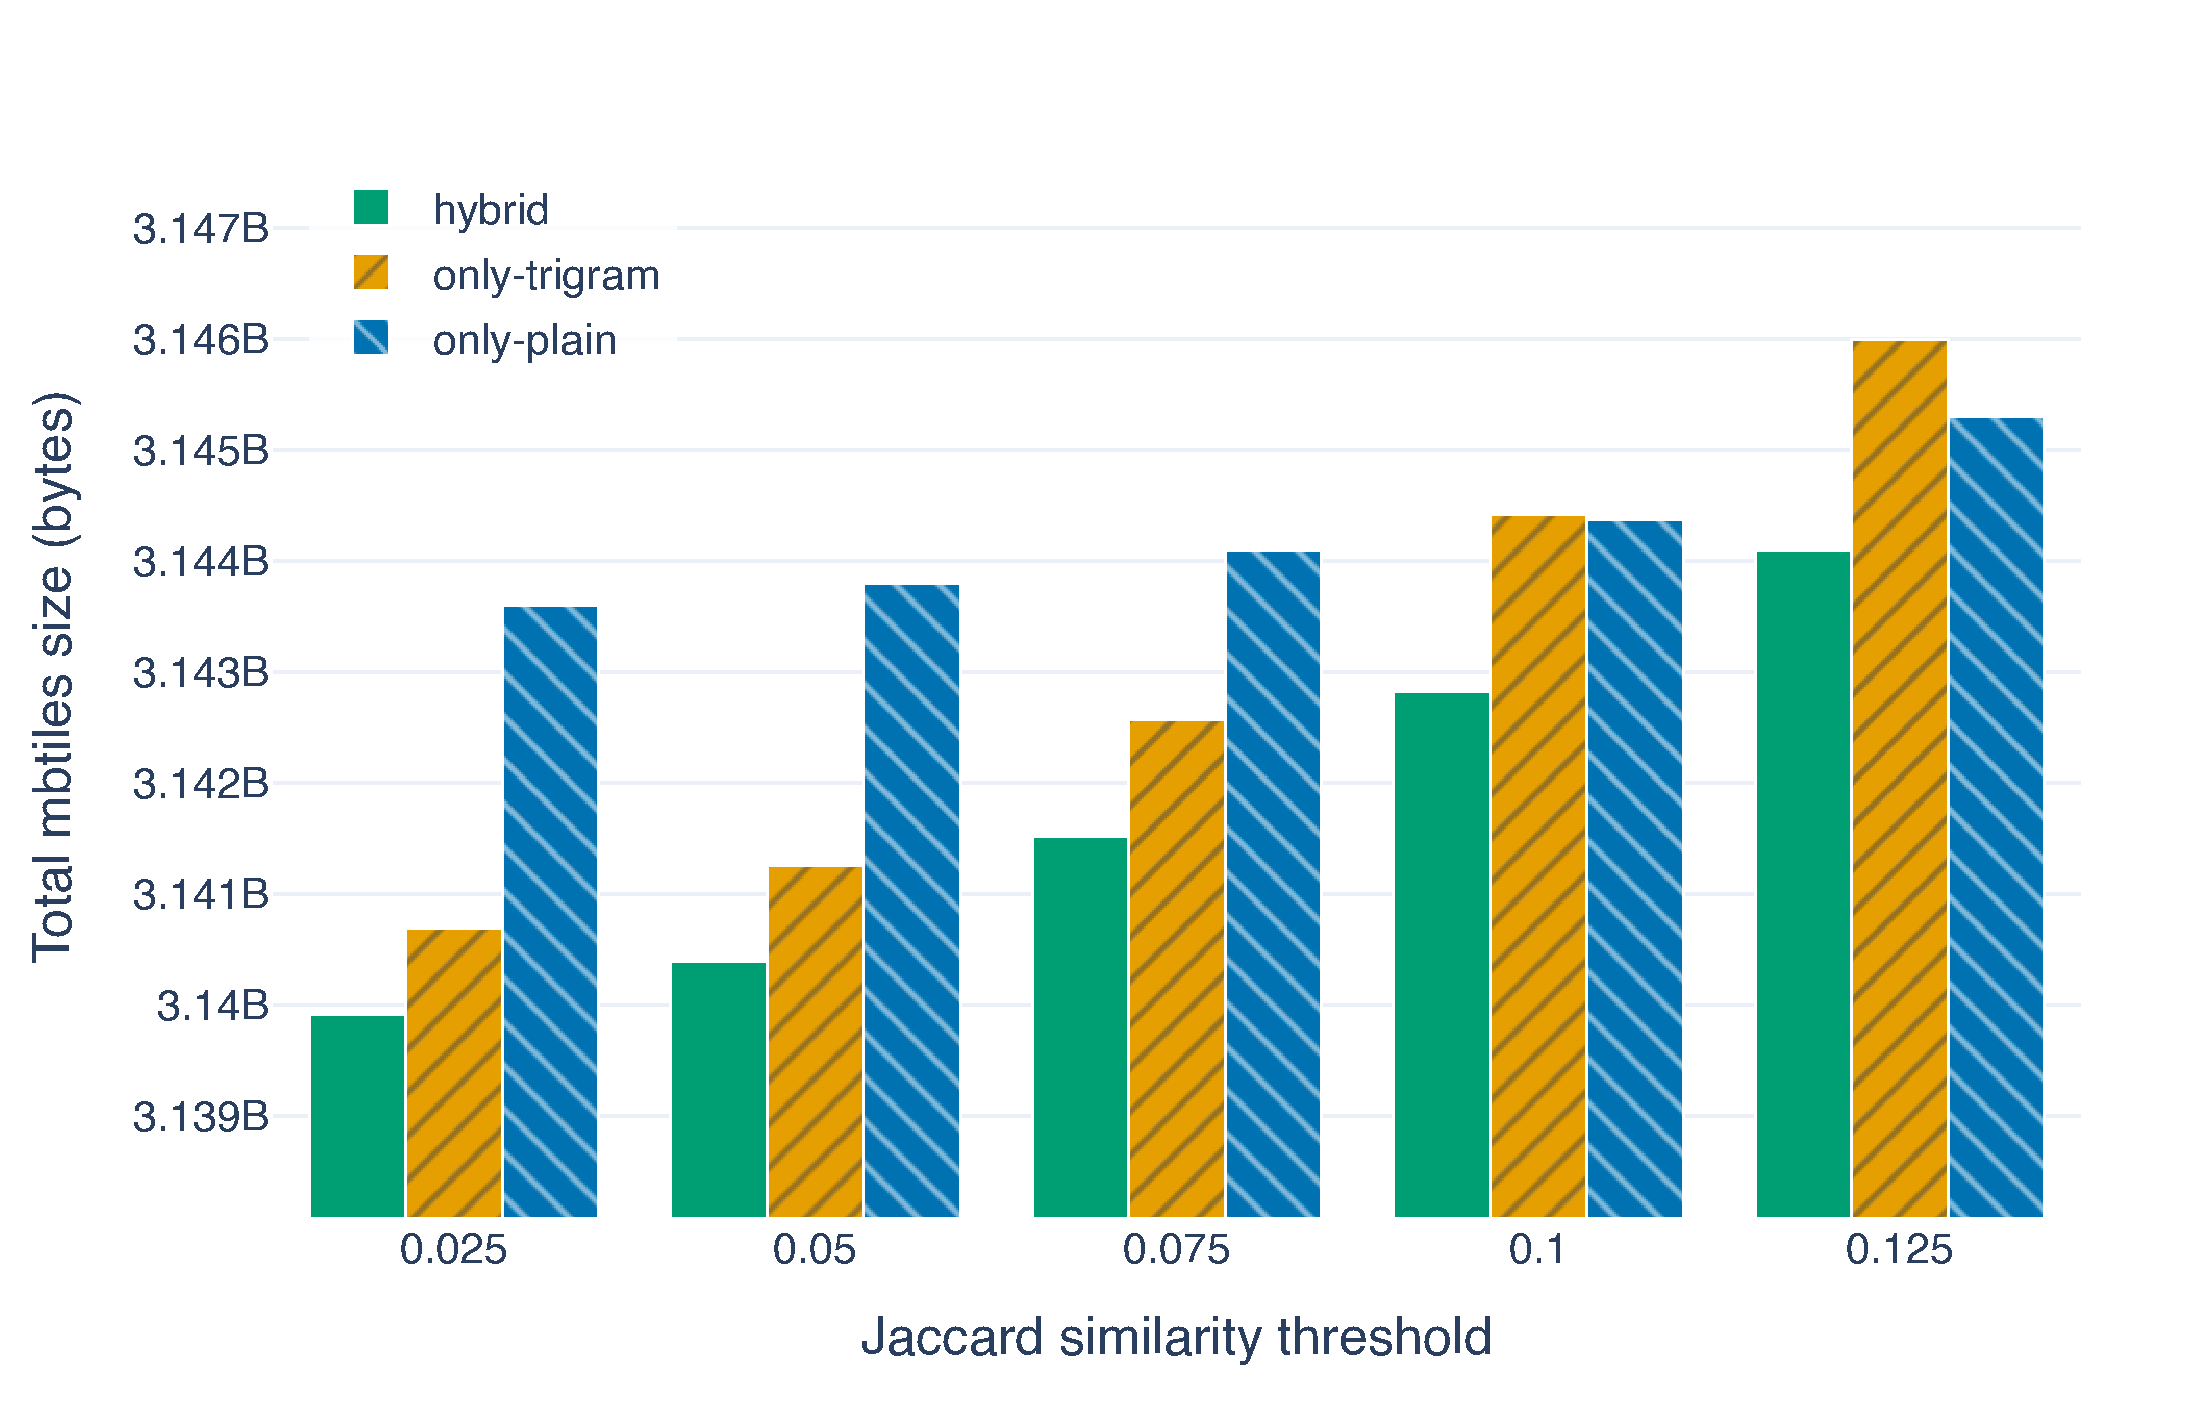
\includegraphics[width=0.8\linewidth]{figures/minhash_sweep.pdf}
    \caption{
Total encoded mbtiles size of the Germany OpenMapTiles tileset under different MinHash similarity modes and Jaccard thresholds.  Lower is better.  The hybrid mode (teal) produces the smallest output at every threshold.
All modes increase monotonically with threshold as fewer column pairs qualify for shared-dictionary grouping.
The y-axis is zoomed to the data range to make the differences visible: the full range spans approximately \qty{6}{\mega\byte} out of \qty{3.14}{\giga\byte} total}
    \label{fig:minhash_sweep}
\end{figure}

\printacronyms[name=Acronyms]
\listoffigures
\listoftables
\begin{sloppypar}
\printbibliography
\end{sloppypar}

\end{document}
